% EPL master thesis cover template
\documentclass{eplmastersthesis}
%!TEX root = /home/renaud/Documents/EPL/tfe/latex/tfe.tex
\RequirePackage{amsmath,amsfonts,amssymb,amsthm}
\RequirePackage{gensymb}
%\RequirePackage{epstopdf}
\RequirePackage{pgfplots}	
\RequirePackage{float}
\RequirePackage[font=small,labelfont=bf]{caption}
\RequirePackage[font=small,labelfont=bf]{subcaption} % [font=footnotesize,labelfont=bf]{subcaption}
\RequirePackage{enumitem}
%\RequirePackage{vwcol} 
\RequirePackage{cases}
\RequirePackage{mathtools}
\RequirePackage{pgfplots}
\pgfplotsset{compat=1.13}
\RequirePackage{tikz}
\usetikzlibrary{patterns,positioning,shapes,shadows,arrows}
%\RequirePackage{tabularx}
\RequirePackage[hidelinks]{hyperref}
% \hypersetup{
%      colorlinks   = true,
%      linkcolor 	  = blue,
%      citecolor    = gray
% }
\RequirePackage{textcomp} 
\RequirePackage{empheq}
\RequirePackage{environ} % provide scaletikzpicturetowidth
\RequirePackage{dsfont}
\RequirePackage{matlab-prettifier}
% \usepackage{algorithm}
% \usepackage{algpseudocode}
% \usepackage{multicol}
\RequirePackage{multirow}
\RequirePackage{booktabs}
\RequirePackage{tcolorbox}
\RequirePackage{minted}
% \usepackage{wrapfig}
\RequirePackage{relsize}
\RequirePackage{slantsc}
\RequirePackage{nextpage}
% custom toc :
\RequirePackage[titles]{tocloft}
\RequirePackage[nottoc]{tocbibind}
\RequirePackage[noadjust]{cite}
%!TEX root = /home/renaud/Documents/EPL/tfe/latex/tfe.tex
\DeclarePairedDelimiter{\ceil}{\lceil}{\rceil}
\DeclarePairedDelimiter{\floor}{\lfloor}{\rfloor}


\newcommand{\G}{\ensuremath{G(\b{x},t,t')}}
\newcommand{\N}{\ensuremath{\mathbb{N}}}
\newcommand{\E}{\ensuremath{\mathbb{E}}}
\newcommand{\R}[1][]{\ensuremath{\mathbb{R}^{#1}}}
\newcommand{\esp}[1]{\ensuremath{\left\langle #1 \right\rangle}}
\newcommand{\p}[1]{\ensuremath{\left( #1 \right)}}
\newcommand{\cppcode}[1]{\mintinline[style=tango]{c++}{#1}}
\newcommand{\Z}{\ensuremath{\mathbb{Z}}}
\newcommand{\M}{\ensuremath{\mathcal{M}}}
\newcommand{\C}{\ensuremath{\mathcal{C}}}
\newcommand{\I}{\ensuremath{\b{(I)\!}}}
\renewcommand{\S}{\ensuremath{\b{(S)\!}}}
\newcommand{\bI}{\ensuremath{\b{(bI)\!}}}
\renewcommand{\P}{\ensuremath{\mathcal{P}}}
\newcommand{\hx}{\ensuremath{\Delta x}}
\newcommand{\hy}{\ensuremath{\Delta y}}
\newcommand{\ex}{\ensuremath{\hat{\b{e}}_x}}
\newcommand{\ey}{\ensuremath{\hat{\b{e}}_y}}
\newcommand{\ez}{\ensuremath{\hat{\b{e}}_z}}
\newcommand{\n}{\ensuremath{\hat{\b n}}}
\newcommand{\nby}{\ensuremath{n_{box,\,y}}}
\newcommand{\nbz}{\ensuremath{n_{box,\,z}}}
\renewcommand{\div}{\ensuremath{\nabla \cdot}}
\newcommand{\rot}{\ensuremath{\nabla \times}}

\makeatletter
\newcommand{\subalign}[1]{%
  \vcenter{%
    \Let@ \restore@math@cr \default@tag
    \baselineskip\fontdimen10 \scriptfont\tw@
    \advance\baselineskip\fontdimen12 \scriptfont\tw@
    \lineskip\thr@@\fontdimen8 \scriptfont\thr@@
    \lineskiplimit\lineskip
    \ialign{\hfil$\m@th\scriptstyle##$&$\m@th\scriptstyle{}##$\crcr
      #1\crcr
    }%
  }
}
\makeatother
%C++
\newcommand{\Cpp}{C\nolinebreak[4]\hspace{-.05em}\raisebox{.4ex}{\relsize{-3}{\textbf{++}}} }
\DeclareMathOperator{\diag}{diag}
\DeclareMathOperator{\VI}{VI}
\DeclareMathOperator{\trace}{trace}
\DeclareMathOperator{\Exp}{e}
\DeclareMathOperator{\cov}{cov}
\DeclareMathOperator*{\argmin}{arg\,min}
\def\mslim{\qopname\relax m{\text{ms-lim}}}
\renewcommand{\t}{\intercal} %transposed matrices

\renewcommand{\rm}{\mathrm}
\renewcommand{\b}{\mathbf}
\newcommand{\bs}{\boldsymbol}
\newcommand{\matlab}{\textsc{Matlab}\up{\textcopyright} }
\newcommand{\mtlb}[1]{\lstinline[style=Matlab-editor]!#1!}

\providecommand{\e}[1]{\ensuremath{\!\times\!10^{#1}}}

\newcommand\blankpage{\null \thispagestyle{empty} \newpage} %\addtocounter{page}{-1}

\makeatletter
\newcommand{\neutralize}[1]{\expandafter\let\csname c@#1\endcsname\count@}
\makeatother
\newtheorem{property}{Property}[section]
\newtheorem{cor}{Corollary}

\newenvironment{propertybis}[1]{
    \renewcommand{\theproperty}{\ref{#1}$'$}%
    \neutralize{property}\phantomsection
    \begin{property}}
    {\end{property}
}

\newenvironment{propertyter}[1]{
    \renewcommand{\theproperty}{\ref{#1}$''$}%
    \neutralize{property}\phantomsection
    \begin{property}}
    {\end{property}
}

\newenvironment{corollary}[1]{
    \renewcommand{\thecor}{\ref{#1}}%
    \neutralize{property}\phantomsection
    \begin{cor}}
    {\end{cor}
}

% Custom toc
\AtBeginDocument{\renewcommand\contentsname{Table of Contents}}
% \setlength{\cftbeforechapskip}{.1ex}
\setlength{\cftbeforesecskip}{-.5ex}
\setlength{\cftbeforesubsecskip}{-1ex}
% \titleformat{\chapter}[display]
% {}{\hfill\rule{.7\textwidth}{3pt}}{0pt}
% {\hfill\huge\bfseries}[\addvspace{-1pt}]
\input{misc/formatting}
% Fill in here the information: title, student name, speciality, jury members
\title{Complex Network Analysis for Marine Models}	% Master thesis title
\subtitle{Subtitle (optional)}			% Optional subtitle
\author{Renaud \textsc{Dufays}}	% Student name
%\secondauthor{Firstname \textsc{Lastname}}	% Second student name if applicable
\speciality{Mathematical Engineering}		% Speciality (use one of the following options):
										% Biomedical Engineering
										% Chemical and Materials Engineering
										% Civil Engineering
										% Computer Science
										% Computer Science and Engineering
										% Electrical Engineering
										% Electro-mechanical Engineering
										% Mathematical Engineering
										% Mechanical Engineering
										% Physical Engineering
%\options{Option(s)}		% If required by program commission mention options
\supervisor{Eric \textsc{Deleersnijder}}	% 1st supervisor name
\cosupervisor{Jean-Charles \textsc{Delvenne}}	% 2nd supervisor name if applicable
\readerone{Laurent \textsc{Delannay}}		% 1st reader name
%\readertwo{Firstname \textsc{Lastname}}		% 2nd reader name
%\readerthree{Firstname \textsc{Lastname}}	% 3rd reader name
\years{2016-2017}	% Academic year

\begin{document}
\pagenumbering{alph}
\renewcommand{\thepage}{C\arabic{page}}
\maketitle					% To create front cover page
% \thispagestyle{empty}		% To suppress header and footer on the back of the cover page
% \null \newpage
% \blankpage
\cleardoublepage
\pagenumbering{roman} % for table of contents, etc.
% \frontmatter
\addcontentsline{toc}{section}{Acknowledgements}
\section*{Acknowledgements}
\tableofcontents
\null \newpage
\addcontentsline{toc}{section}{List of abbreviations and symbols}
\section*{List of abbreviations and symbols}
\null\newpage
\cleartooddpage
\pagenumbering{arabic}
% \mainmatter
%!TEX root = /home/renaud/Documents/EPL/tfe/latex/tfe.tex
\addcontentsline{toc}{chapter}{Introduction}
\chapter*{Introduction}
The understanding of geophysical and environmental fluid flows has shown an increasing interest over the past decades. Climate change, and the related issue of pollution have raised the need for accurate simulations allowing to understand and predict the time-space evolution of the concentration of pollutants in the environment. In this regard, the fate of constituents dissolved in a fluid mixture is commonly modelled by means of reactive-transport equations. Those are coupled partial differential equations taking into account the influence of \textit{reactions} as well as of the advective and diffusive \textit{transport phenomena} on the concentration of the constituent in the mixture. Accurate algorithms have been developed by engineers to numerically solve such equations. Finite differences, finite volume and finite elements methods are amongst the most commonly used discretization methods. However, they rely on grids containing thousands and in some instances millions of grid points so that CPU time can become prohibitive in cases where long time simulations are needed. Furthermore, although those methods provide pretty accurate results, these often suffer from a lack of \textit{interpretation}. This raises the need for simpler models with a few number of variables that would allow for an easier interpretation of the results as well as for fast long time simulations. Obviously, one cannot expect such models to provide results that would be as accurate as the ones furnished by the previously mentioned methods. Hence, both approaches are complementary. 

One way to build such coarser models is to partition the domain of interest into a relatively small number of subdomains, called \textit{compartments} or \textit{boxes} over which the state variables are assumed \textit{homogeneous}. The fluxes between the compartments are then expressed by simple laws, leading to models that are relatively easy to interpret. This procedure leads to models called \textit{compartment models} or equivalently \textit{box models}. The number of subdomains and their shapes vary widely from one problem to another. Some schematic representations of compartment models found in the literature are shown in figure~\ref{fig:intro:boxmodels}.

Box models have been widely used in studies involving marine systems as well at local scale \cite{deleersnijder1998two,maderich2014regional,soetaert1995estimating} as at global scale \cite{kohler2005quantitative,munhoven1996glacial}. The choice of the subdomains and the specification of the fluxes exchanged between them rely on ad-hoc or empirical methods, based on the known hydrodynamics over the domain considered. It seems that no automatic procedure exists to define a relevant partitioning of the domain. The goal of this work is thus to fill that gap by proposing a method based on the tools of \textit{network science} to automatically delineate relevant compartments.

Network science may be defined as the study of graphs (or networks) and their use to model various (real-life or not) problems. Informally, a graph is a mathematical representation of a set of objects (the \textit{nodes} or \textit{vertices} of the graph), and the links between pairs of them (the \textit{edges} of the graph). The field of application of network science is extremely large, as illustrated by this quote from Newman \cite{newman2010networks}: "\textit{Many objects of interest in the physical, biological, and social sciences can be thought of as networks and [...] thinking of them in this way can often lead to new and useful insights}."
\newpage
Often, graphs exhibit a \textit{community structure}: it is the case if the vertices can be organized into groups such that there are many interactions between the nodes within a group, and few interaction between the nodes of different groups. Such groups of vertices are called \textit{communities} or \textit{clusters}. An example of a three communities partitioning of a simple graph is shown in figure~\ref{fiug:intro:communities}. The art of revealing the community structure of a graph has a long history in network science, and a variety of \textit{community detection algorithms} and \textit{heuristics} has been developed, see \cite{fortunato2010community} for a 2010 survey. Clustering methods have shown to be useful for a wide applications such as social and biological networks \cite{girvan2002community}, biochemical networks \cite{holme2003subnetwork,guimera2005functional,palla2005uncovering}, or informations networks such as the world wide web \cite{flake2002self}. What makes communities particularly appealing is that they often correspond to \textit{functional units} such as cycles or pathways in metabolic networks \cite{guimera2005functional,palla2005uncovering,huss2007currency} or collections of pages on a single topic on the web \cite{flake2002self}. In the context of geophysical modeling, clustering methods have been used in works providing suggestions for the optimal placement of marine protected areas \cite{thomas2014numerical,jacobi2012identification,rossi2014hydrodynamic}. In this work, we aim to show that communities may correspond to relevant compartments in the case of advection-diffusion flow networks. To this end, we focus on one relatively recent method for community detection based on the \textit{stability} measure \cite{delvenne2010stability,delvenne2013stability,lambiotte2009laplacian}.

A complete procedure is proposed to build a compartment model from any problem whose velocity field and diffusivity tensor are known. First, the Lagrangian equations describing individual particles trajectories are derived from the transport model, and consistent numerical methods are proposed. This allows to compute the transition probability matrix at the desired times, which is the information needed to apply the stability clustering method. Finally, subdomains are delineated from the communities found by the clustering algorithm, and the exchange coefficients between the compartments are estimated numerically, completing the construction of the box model. This approach may be viewed	as a special application of the theory of model order reduction~\cite{deleersnijder2009reduction}. The whole procedure is applied on a simple, two dimensional test problem, and the resulting box model is assessed.  

The first part of the work gathers all the theoretical tools needed for that procedure. Chapter~\ref{chap:clustering} is devoted to community detection and in particular to the \textit{stability} measure and the related clustering algorithm. The reactive transport equation and the study of its properties is the topic of chapter~\ref{chap:transportmodel}, whereas compartment models and their properties are studied in chapter~\ref{chap:compartment}. Then, the link between the transport model and the Lagrangian equations describing the position of an individual particle is shown in chapter~\ref{chap:numerical}, leading to the theory of stochastic differential equations and of the consistent numerical methods to solve them. The second part of this work consists in applying the procedure on a simple problem. An idealized, two-dimensional overturning circulation model is presented in~\ref{chap:overturnercirculation} and is then used the build the test problem in chapter~\ref{chap:bioverturner}. The complete procedure is applied on that test problem and assessed in the same chapter. 


\begin{figure}[!htp]
	\begin{subfigure}[t]{.47\linewidth}
		\centering
		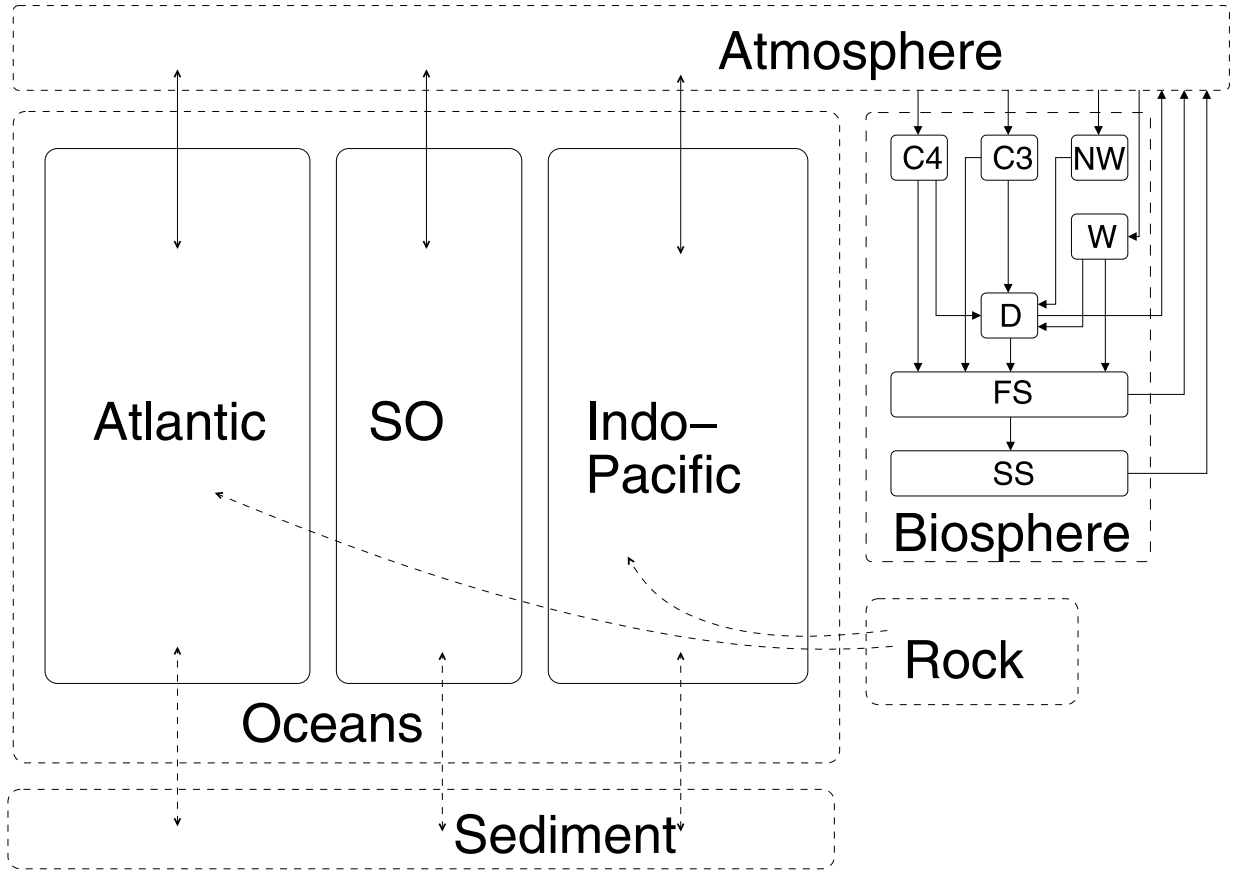
\includegraphics[width=\textwidth]{fig/intro/boxmodel_KohlerEtAl.png}
		\caption{Geometry of the box model of the isotopic carbon cycle (BICYCLE), where the arrows represent carbon fluxes between the compartments. This is figure 1 of \cite{kohler2005quantitative}.}
	\end{subfigure}
		\begin{subfigure}[t]{.51\linewidth}
		\centering
		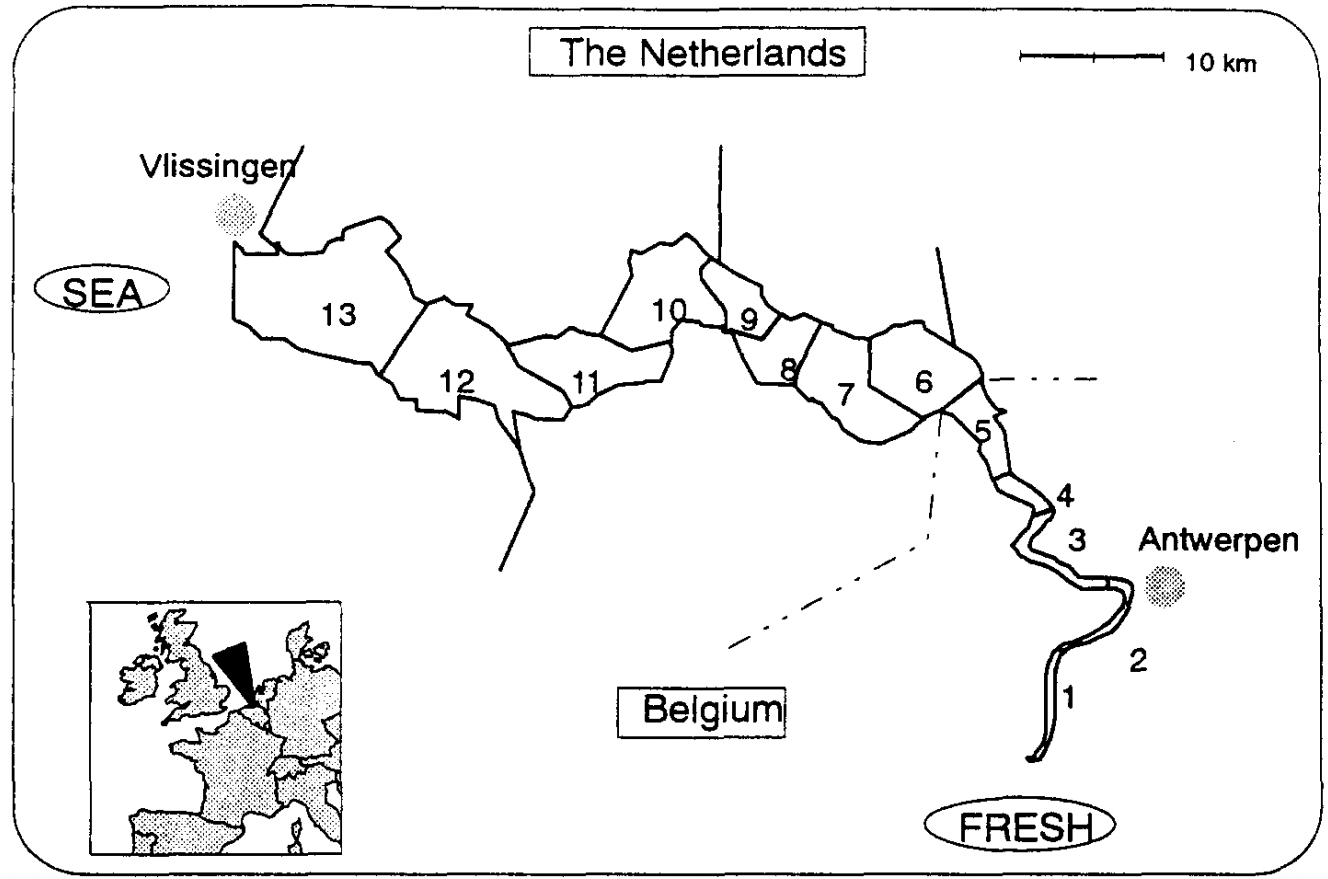
\includegraphics[width=\textwidth]{fig/intro/boxmodel_SoetaertHerman.png}
		\caption{Representation of a subdomain decomposition of the Westerschelde. This is figure 1 of \cite{soetaert1995estimating}.}
	\end{subfigure}
	\begin{subfigure}[b]{\linewidth}
		\centering
		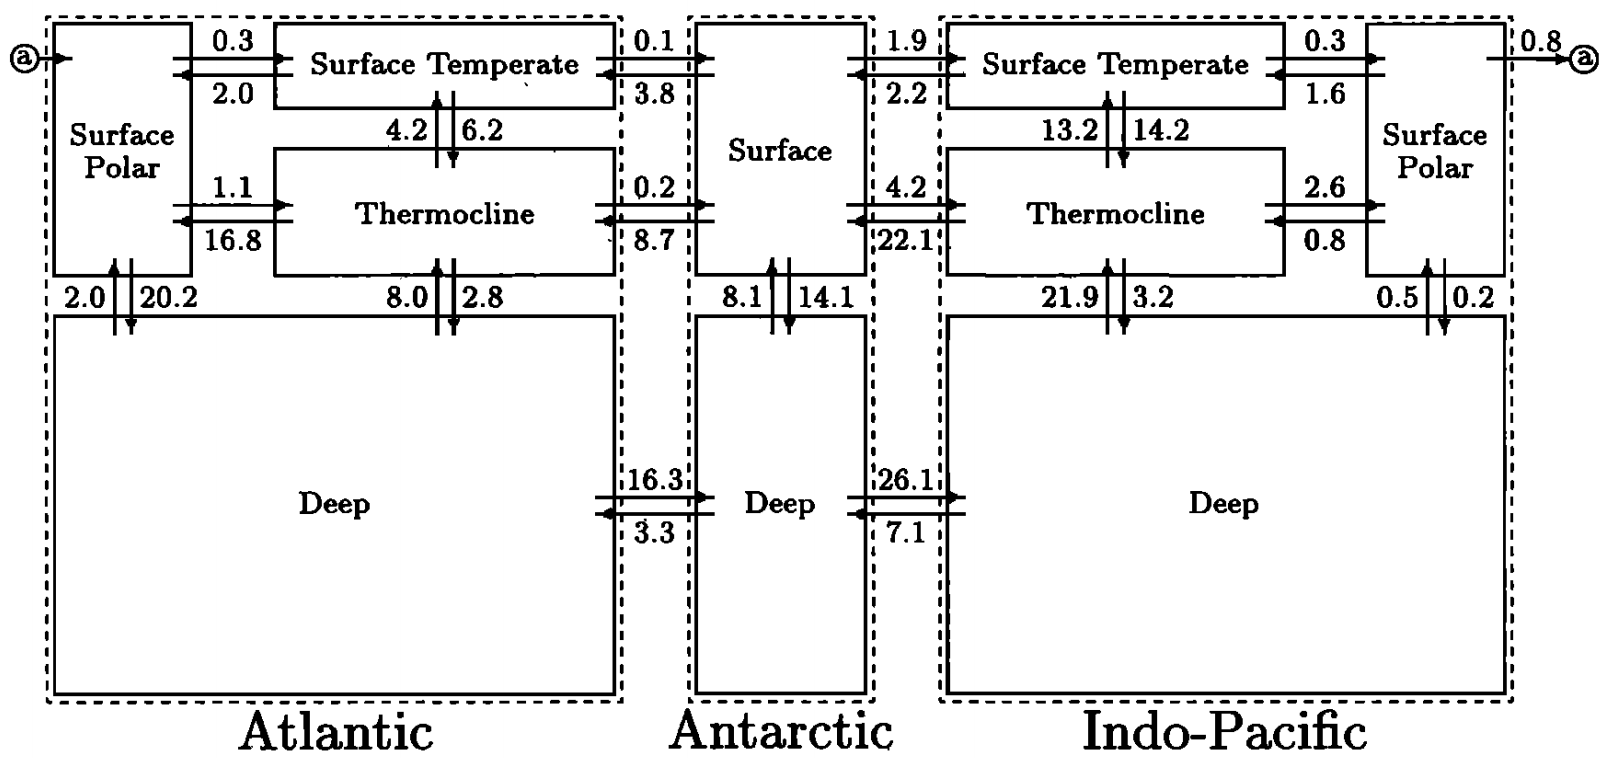
\includegraphics[width=\textwidth]{fig/intro/boxmodel_Munhoven.png}
		\caption{Geometry and water fluxes of a compartmental model for the World Ocean. The fluxes are expressed in sverdrups ($1$ Sv = $10^6$ $\rm{m^3/s}$). This is figure 3 of \cite{munhoven1996glacial}.}
	\end{subfigure}%
\caption{Schematic representations of different compartment models.}\label{fig:intro:boxmodels}
\end{figure}
\begin{figure}[!htp]
	\centering
	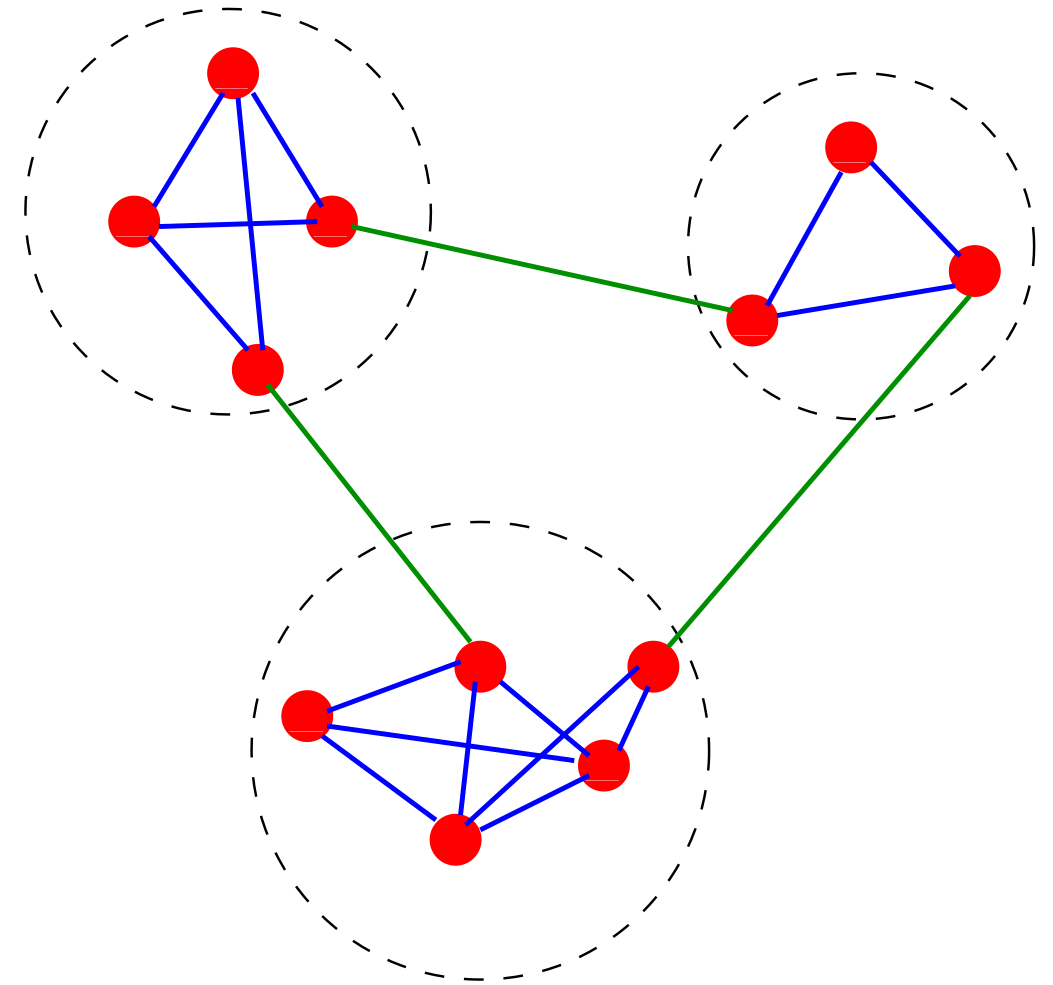
\includegraphics[width=.4\textwidth]{fig/intro/communities_example.png}
	\caption{Example of a three-communities partitioning on a simple network.} \label{fiug:intro:communities}
\end{figure}
\part{Theoretical}
%!TEX root = ../tfe.tex
\chapter{Clustering}
\section{The stability criterion for graph communities} \label{sec:stability}
The partition of a graph into communities (or clusters) as been widely studies those last two decades. Clustering comes indeed pretty handy to gain insight into the underlying structure of a system represented by a network. In some casesbuild a simplified functional description based on the clusters. Many partitioning methods have been proposed, each relying on a particular measure to quantify the quality of a community structure. Such methods include normalized cut, ($\alpha$,$\epsilon$) clustering or modularity and its variants and extensions. See for instance \cite{fortunato2010community} for a 2010 survey. In this work, we choose the stability approach, which is based on the statistical properties of a dynamical process taking place on the network. This approach was initially presented in \cite{delvenne2010stability} and further expended in \cite{lambiotte2009laplacian} and \cite{delvenne2013stability}. 

The stability method presents a number of advantages. First, it does not require the number of communities to be specified beforehand, ensuring a natural partitioning of the graph. Second, it is flexible in the sense that it does not seek a \textit{unique} optimal partition. Instead, it reveals several community structures, each appearing to be the most relevant at particular values of the Markov time: at a given time scale, natural clusters corresponds to sets of states from which escape is unlikely within that time scale. The stability method provides thus a dynamical interpretation of the partitioning problem. The Markov time acts as an intrinsic resolution parameter, as will be developed shortly. Finally, it is probably the most unifying approach since many of the standard partitioning measures find an interpretation through the stability framework.

In order to compute stability partitions in the next of this work, we make use of Michael Schaub's free software \textit{PartitionStability}. This C++ implementation of the stability method with a \matlab interface is available at \url{https://github.com/michaelschaub/PartitionStability}. It relies on the Louvain algorithm \cite{blondel2008fast} to optimize the stability quality function. This heuristic algorithm has been initially developed for modularity optimisation. However one can show that stability can be written as the \textit{modularity} of a time-dependent network evolving under the Markov process \cite{lambiotte2009laplacian}. Hence, the Louvain method can almost straightforwardly be applied to stability optimisation.

This section is devoted to the explanation of the stability measure, and how to find good clusterings using stability analysis. This theoretical part is intended to cover everything that is needed to make a proper, informed use of the stability toolbox. The stability measure has initially been presented for dicrete times in \cite{delvenne2010stability}. We follow the same approach here : discrete-time stability is developed in the first part of this section; it is then extended to continuous time in a second part; finally, a few tools to analyze the robustness of a partition are presented in the third part of the section.

\subsection{Discrete-time stability as an autocovorariance}
The stability criterion is based on the two-way relationship between graphs and Markov chains: On one hand, any graph has an associated Markov chain where the states are the nodes of the graph and the transitions probabilities between states are given by the weights of the edges. On the other hand, any Markov chain can be represented by a graph whose edges are weighted according to the transition probabilities. Concretely, consider a graph of $N$ nodes whose $N \times N$ weighted adjacency matrix is denoted $\b A$. Let $\b k = \b A \b 1$; $k_i$ is thus the total weight of the outgoing edges from node $i$. Let $\b K = \mathrm{diag}(\b k)$. Then, by normalizing the rows of $\b A$ we get the matrix $\b M = \b K^{-1}\b A$, the transition probability matrix. $\b M$ is row-stochastic (or right-stochastic) and $[\b M]_{ij}$ is the probability to go from node $i$ to node $j$. 
Consider a particle moving in the network according to the transition probabilities in $\b M$. Now let $\b p_t$ be the $1 \times N$ probability vector at Markov time $t$, namely that $p_{t,i}$ is the probability that the particle is located in node $i$ at time $t$. The dynamics of the discrete-time Markov process are given by :
\begin{equation} \label{eq:discreteMP}
	\b p_{t+1} = \b p_t \b K^{-1}\b A = \b p_t \b M.  	
\end{equation} 
Now, suppose that the Markov chain is ergodic, i.e. that it is possible to go from every state to every state and that the Markov process is aperiodic. The ergodicity assumption implies that any initial state will asymptotically reach the same stationary solution. Let $\bs \pi$ be that stationary distribution, given by $\bs \pi = \bs \pi \b M$, and $\b \Pi = \rm{diag}(\bs \pi)$. Now, let $\b x_t$ be the $N$-dimensional random indicator vector describing the position of a particle undergoing the above dynamics : $x_{t,i} = 1$ if the particle is located in node $i$ at time $t$, and $0$ otherwise. At stationarity, the \textit{autocovariance matrix} of $\b x$ is
\begin{align}
 	\b C(\b x_\tau,\b x_{\tau+t}) &\triangleq \E\left[(\b x_\tau - \E[\b x_\tau])^{\t}(\b x_{\tau+t} - \E[\b x_{\tau+t}])\right] \\
 		&= \E\left[(\b x_\tau - \bs \pi)^{\t}(\b x_{\tau+t} - \bs \pi)\right] \\
 		&= \E\left[\b x_\tau^{\t} \b x_{\tau+t}\right] - \E[\b x_{\tau}^{\t}] \bs \pi - \bs \pi^{\t} \E\left[\b x_{\tau+t}\right] + \bs \pi^{\t} \bs \pi \\
 		&= \bs \Pi \b M^t - \bs \pi^{\t} \bs \pi,
 \end{align}
 where the fact that $\b C(\b x_\tau,\b x_{\tau+t})$ only depends on the time difference $t$ at stationarity is readily verified. Here, $^\t$ is the transposed sign and $\b M^t$ is $\b M$ at the power $t$. $[\b C(\b x_\tau,\b x_{\tau+t})]_{ij}$ is interpreted as the correlation between $\b x_{\tau,\,i}$ and $\b x_{\tau+t,\,j}$. The independence on the initial time $\tau$ implies that it can indifferently be chosen equal to $0$.

Suppose now a partition $\P$; we note $\b H_{\P}$ the indicator matrix of $\P$. If $c$ is the number of communities in $\P$, $\b H_{\P}$ is a binary $N \times c$ matrix such that 
\begin{equation}
	[\b H_{\P}]_{ik} = 
	\begin{cases}
		1  & \quad \mbox{if node $i$ is in community $k$},\\
	    0  & \quad \text{otherwise}.\\
	\end{cases}
\end{equation}
Let us define $\mathcal{H}_{\P} : \R[N \times N] \rightarrow \R[c \times c] : \b B \mapsto \mathcal{H}(\b B) = \b H_{\P}^{\t} \b B \b H_{\P}$. Let $\b X$ be any $N \times N$ matrix, then $\b Y = \mathcal{H}_{\P}(\b X)$ is a $c \times c$ matrix such that $[\b Y]_{kl} = \sum_{i \in \C_k,\, j \in \C_l} [\b X]_{ij}$, where $\C_k$ and $\C_l$ denote communites $k$ and $l$ of partition $\P$. One could thus say that operator $\mathcal{H}_{\P}$ returns the \textit{clustered version} of any $N \times N$ matrix, namely the matrix where the contributions of every nodes belonging to the same community are gathered by summing them. Finally, let $\b y_t = \b H_{\P}^{\t} \b x_t$ denote the $c$-dimensional community indicator vector: $\b y_{t,\,k}$ is equal to $1$ if the particle is in community $k$ at time $t$ and zero otherwise.
Using those notations and the interpretation of $\mathcal{H}_{\P} $, the \textit{clustered autocovariance matrix} for partition $\P$ at time $t$ is defined as
\begin{align}
	\b R_t(\P) &= \mathcal{H}_{\P}\left(\b C(\b x_\tau,\b x_{\tau+t})\right)\\
		&= \b C(\b y_\tau,\b y_{\tau+t})\\
		&= \b H_{\P}^{\t}(\b \Pi\b M^t - \bs \pi^{\t}\bs \pi)\b H_{\P}.
\end{align}
Notice that $\b R_t$ depends only on the topology of the graph and on the partition. If the graph has well defined communities given by $\P$ \textit{over a given time scale}, we expect that the particle is more likely to remain within the starting community overt that time scale. This implies that the values of $\b y_{0,\,i}$ and $\b y_{t,\,i}$ are positively correlated for $t$ in that time scale, which in turn implies large diagonal elements in $\b R_t(\P)$ and hence a large trace of $\b R_t(\P)$. The elements of $\b R_t(\P)$ are interpreted as follows in terms of the random walk of a particle : $[\b R_t(\P)]_{kl}$ is the probability that a particle is in community $\C_l$ after $t$ discrete time-steps if it has started in $\C_k$ minus the probability that two independant random walkers are in $\C_k$ and $\C_l$, evaluated at stationarity. A good partition is such that there is a high likelyhood of remaining in the starting community over a given time scale. The definition of the stability of a \textit{clustering} $\P$ follows naturally:
\begin{equation}
	r_t(\P) = \min_{0 \le s \le t} \sum_{i = 1}^{c} [\b R_s]_{ii} = \min_{0 \le s \le t} \trace(\b R_s).
\end{equation}
Note that taking the minimum for all times up to $t$ implies that the stability of the clustering at time $t$ is large only if it is large for all times preceding $t$. This allows to assign a low stability to partitions where there is a high probability of leaving the community and coming back to it later. According to \cite{delvenne2013stability}, this minimisation is unnecessary in most cases and we have $r_t(\P) \approx \trace(\b R_t)$. Nevertheless, taking the minimization ensures maximum generality and allows for example to deal with almost bipartite graphs where $\trace(\b R_s)$ can be oscillatory.
The definitions above stands all for a given partition $\P$. As we are interested in the optimal clustering in the sense of stability, we search the partition that maximize the stability. Clearly, the optimal partition might be different for each Markov time $t$. Computing the optimal partition for each Markov time gives the \textit{stability curve of the graph} :
\begin{equation}
	r_t = \max_{\P} r_t(\P).
\end{equation}
We understand thus how Markov time acts as an intrinsic resolution parameter: as Markov time grows, the number of communities is expected to decrease, since there are more possibilities for a random walker to escape a community when the time window increases. Hence, communities get bigger (or coarser) with Markov time increasing. Interestingly, one can prove that in the case of \textit{undirected} networks, stability at time 1 is equivalent to the well-known \textit{configuration modularity} measure. But this equivalence does not hold for \textit{directed} networks and therefore does not concern the present work.

At this stage, an important remark has to be made about the assumption of ergodicity. The verification of this assumption is often far from being obvious, especially in the case of big undirected networks. The trick in that case is to introduce "à la Google" random teleportations.\footnote{In the original PageRank proposed by S. Brin and L. Page in 1998 (ref. \cite{grin1998anatomy}), this consist essentially in applying a perturbation to the transition probability matrix between web pages in order to ensure that at least one row of the matrix is positive, which implies the convergence of the Power Method. If we note the teleportation probability $\tau$, the perturbation can be interpreted as follows: a web surfer follows a link in his current page with probability $1-\tau$ and jumps to an arbitrary web page with probability $\tau$.} Let $\tau$ be the \textit{teleportation probability}. Then, if a random walker is located on a node with at least one outlink (which is always the case for the networks that we will consider), it follows one of the outlinks with probability $1-\tau$. Otherwise, the node is called a \textit{dangling node} and the random walker is teleported with a uniform probability to another random node. The corresponding perturbation of the transition probability matrix is, in the most general case:
\begin{equation} \label{eq:M_teleport}
	\widetilde{\b M} = (1-\tau)\b M + \frac{1}{N}[(1-\tau)\b d + \tau \b 1]\b 1^{\t},
\end{equation}
where $N$ is the number of nodes, $\b d$ is a binary $N \times 1$ vector whose entries are equal to $1$ if the corresponding node is a dangling node and $0$ otherwise, and $\b 1$ is the $N \times 1$ unity vector. In the case that we will consider in the next section, $\b d$ is the zero vector. This perturbation is known to make the dynamics ergodic, ensuring the existence and uniqueness of the stationary solution $\bs \pi$.

\subsection{Extension to continuous time}
From a general viewpoint, the discrete process can be interpreted as an approximation of its continuous counterpart : whereas the state of the discrete-time random walker can only change at unit-time intervals, the continuous-time random walkers undergoes a waiting time between each change of state which is itself a random variable. More precisely, it is a continuous memoryless random variable distributed exponentially. Obviously, the transition probabilities from one node to the other are the same for both discrete- and continuous-time processes, only the time at which the jump occurs may vary. The continuous-time process corresponding to \eqref{eq:discreteMP} is governed by the following dynamics :
\begin{equation} \label{eq:continuousMP_general}
    	\dot{\b p} = \b p \diag\left\{\bs \lambda(\b k)\right\} \b K^{-1} \b A - \b p \diag\left\{\bs \lambda(\b k)\right\} = -\b p \b L,
\end{equation}
where $\lambda_i(\b k)$ is the rate at which random walkers leave node $i$, and $\b L = \diag\{\bs \lambda(\b k)\}[-\b K^{-1} \b A + \b I]$. Two particular cases of this process are implemented by the stability software and are thus examined here, depending on the choice of $\bs \lambda(\b k)$ : the so-called \textit{normalised Laplacian dynamics} and \textit{standard (combinatorial) Laplacian dynamics}. Their names comes from the similarity that arise between $\b L$ and the normalied/standard Laplacian matrix. Each of those two dynamics represent best different physical processes. The former correspond to the choice $\bs \lambda_{norm}(\b k) = \b 1$. Hence, the expected waiting time is $1$ at every node, and $\b L = -\b K^{-1} \b A + \b I = -\b M + \b I$. The latter corresponds to $\bs \lambda_{combi}(\b k) = \b k/\langle \b k \rangle$. In that case, $\b L = (-\b A + \b K)/\langle \b k \rangle$ and the average waiting time at node $i$ is $\langle \b k \rangle/k_i$. Hence, the expected waiting time at a given node is smaller (resp. larger) than $1$ if the total weight of the outgoing edges from that node is larger (resp. smaller) than the average total weight of the outgoing edges on the network. However, the expected waiting time over the whole network is $\langle \langle \b k \rangle/\b k \rangle = 1$. The corresponding governing equations are respectively 
\begin{equation} \label{eq:continuousMP_norm}
	\dot{\b p} = \b p \b K^{-1} \b A - \b p = \b p \b M - \b p
\end{equation}
for the normalized Laplacian and
\begin{equation} \label{eq:continuousMP_combi}
    	\dot{\b p} = \b p \frac{\b A}{\langle \b k \rangle} - \b p\frac{\b K}{\langle \b k \rangle}
\end{equation}
for the combinatorial Laplacian.

The clustered autocovariance matrix for partition $\P$ at time $t$ is easily generalised to 
\begin{equation}
	\b R(t;\P) = \b H_{\P}^{\t}(\b \Pi\b P(t) - \bs \pi^{\t}\bs \pi)\b H_{\P},
\end{equation}
where $\b P(t)$ is the the transition matrix of the process at time $t$: $\b P(t) = \Exp^{-t\b L}$. The continuous-time definition of the stability of a partition $\P$ follows almost straightforwardly :
\begin{equation}
	r(t;\P) = \trace \left[ \b R(t; \P) \right].
\end{equation}
Notice that it is not necessary to minimise over the time interval $[0,t]$ : indeed, it can be shown that $\trace \left[ \b R(t;\P) \right]$ is monotonically decreasing with time. The interpretation in terms of a random walk is similar to the discrete case : let $P(\C,t)$ be the probability that a random walker is in community $\C$ at time $t$ if it was initially in $\C$, when the system is at stationarity. Discounting the probability of such an event to take place by chance at stationarity and summing over all communities of $\P$ leads to the definition of the stability of the partition $\P$ :
\begin{equation} \label{eq:generalstability}
	r(t;\P) = \sum_{\C \in \P} P(\C,t) - P(\C,\infty).
\end{equation}
By ergodicity, the memory of the initial condition is lost at infinity and $P(\C,\infty)$ is thus equal to the probability that two independant walkers are in $\C$ at stationarity. Equation \eqref{eq:generalstability} tells us that only the communities in which a random walker is likely to stay brings a positive contribution to stability, where \textit{likely to stay} means that the probability for a walker to be in its initial community at time $t$ is larger than the probability of that event occuring by chance at stationarity. The stability curve of the graph can now be expressed as a continuous function of $t$ :
\begin{equation}
	r(t) = \max_{\P} r(t;\P).
\end{equation}

%----------------------------------------ROBUSTNESS----------------------------------------------------------------%
\subsection{Assessing the robustness of a partition} \label{subsec:robustness}
We present here two mechanisms commonly used to assess the relevance of a particular partition. One simple way is to consider that a robust partition should not be alterred by a small modification of the quality function. Such a modification could be for example a perturbation of the Markov time $t$ at which the partition has been found. From this point of view, robust partitions correspond to \textit{plateaux} in the community curve of the graph. In other words, robust partitions should be persistent over a wide interval of Markov time.

\begin{sloppypar} 
The second indicator of the robustness of a partition that we will take into account in this work follows from considering that a robust partition is one that is persistent to small modifications of the optimization algorithm. The central tool to quantify this approach of the robustness of a partition is the \textit{normalized variation of information} \cite{meilua2007comparing}, which is a popular way to compare two partitions. Let $p(\C)$ be the probability for a node to be in community $\C$, i.e. $p(\C) = n_\C/N$ where $n_\C$ is the number of nodes in community $\C$. The variation of information between partitions $\P_1$ and $\P_2$ is defined by :
\begin{equation} \label{eq:clustering_VI}
	\VI(\P_1,\P_2) := \frac{H(\P_1,\P_2)-H(\P_1)-H(\P_2)}{\log (N)} = \frac{H(\P_1|\P_2)+H(\P_2|\P_1)}{\log (N)},
\end{equation}
where $\log(N)$ is a normalization factor; $H(\P) = -\sum_{\C} p(\C) \log[p(\C)]$ is the Shannon entropy; $H(\P_1,\P_2)$ is the Shannon entropy of the joint probability $p(\C_1,\C_2)$ that a node belongs to both a community $\C_1$ of $\P_1$ and a community $\C_2$ of $\P_2$. This yields $p(\C_1,\C_2) = n_{\C_1 \cap\, \C_2}/N$, and $H(\P_1,\P_2) = -\sum_{\C_1 \in \P_1} \sum_{\C_2 \in \P_2} p(\C_1,\C_2) \log[p(\C_1,\C_2)]$; and $H(\P_1|\P_2)$ is the conditional Shannon entropy of partition $\P_1$ given $\P_2$, which is defined in a standard way from the joint distribution: $p(\C_1|\C_2) = p(\C_1,\C_2)/p(\C_2) = n_{\C_1\cap\, \C_2}/n_{\C_2}$, and the expression of $H(\P_1|\P_2)$ follows straightforwardly. The latter can be interpreted as the additional information needed to describe $\P_1$ once $\P_2$ is known. This measure of the difference bewteen two partition is then used as follows: for each Markov time, an ensemble of Louvain optimisations of stability are performed, starting from different random initial node ordering. Remember that the problem being $\mathcal{NP}$-hard, we rely on a heuristic algorithm --- the Louvain method --- that finds a good partition for a given Markov time, but not necessarily the optimal partition. Hence the partition found may differ if a different initial condition is provided. The normalized variation of information allows then to quantify how different the optimised partitions are. Therefore, a low variation of information indicates optimised partitions that are very similar to each others, hence that a small modification of the algorithm barely alter the partition. From the point of view of the field of dynamical system, robust partitions have thus an attractor with a large basin of attraction for the optimisation method. 
\end{sloppypar}


%-------------------------------------------CLUSTERING OVERTURNER-----------------------------------------------%
\section{Clustering of the overturner problem}
% 1. Expliquer ce qu'on va faire
% 2. Décomposition du domaine en boxes, on cherche ce que donne le clustering sur ces boxes.
% 3. Résultats pour nboxy = 15, nboxz = 10 (et expliquer que ces choix permettent que y0 et z0 correspondent à des frontières de box)

This section presents the results of applying a stability-based community detection algorithm on the overturner problem. First, we explain how the method is applied and then we present the results for a given set of data's.

%-----------------------DESCRIPTION OF THE METHOD---------------------------------%
\subsection{Description of the method}
In order to apply a clustering algorithm on the overturner problem, we have to define how the model can be considered as a graph. To this end, the domain is decomposed into $\nby \times \nbz$ boxes. We note $N_{box} = \nby\nbz$ the total number of boxes. Figure \ref{fig:box_scheme} represents an example of such a domain decomposition with $\nby = 15$ and $\nbz = 10$. For any time $T$, the corresponding directed graph is build as follows : each node represents a box, and the weight of the edge between nodes $i$ and $j$ is the probability $m_{ij}(T)$ that a particle ends up in box $j$ after a time $T$ if it was initially in box $i$. If $m_{ij}(T) = 0$, one can equivalently consider that there is no edge between nodes $i$ and $j$. Since the problem is stationnary, $m_{ij}(T)$ depends only on the elapsed time $T$, not on the initial time. Hence, the initial time can indifferently be considered as being zero. The adjacency matrix $\b M(T)$ of the graph is build from the weights $m_{ij}(T)$: $[\b M(T)]_{ij} = m_{ij}(T)$. For any time $T$, $\b M(T)$ is row-stochastic, i.e. $\b M(T)\b 1 = \b 1$, where $\b 1$ is the $N_{box}$-dimensional unit column vector. The latter has a straightforward physical interpretation: every particle remains in the domain.
\begin{figure}[h!]
	\centering
	% This file was created by matlab2tikz.
%
%The latest updates can be retrieved from
%  http://www.mathworks.com/matlabcentral/fileexchange/22022-matlab2tikz-matlab2tikz
%where you can also make suggestions and rate matlab2tikz.
%
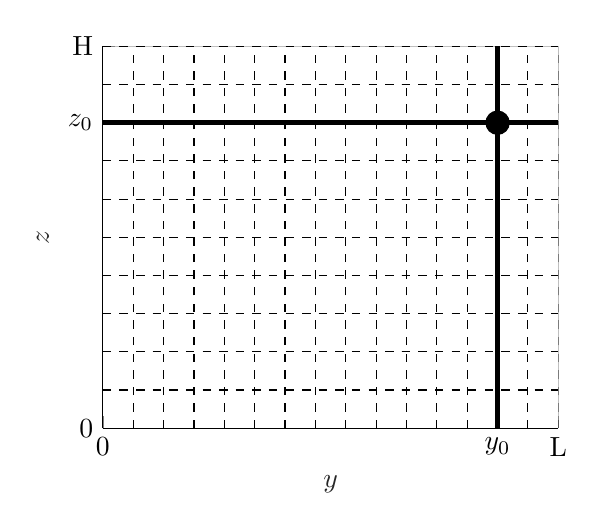
\begin{tikzpicture}

\begin{axis}[%
width=0.477\textwidth,
height=0.4\textwidth,
at={(0\textwidth,0\textwidth)},
scale only axis,
xmin=0,
xmax=15,
xtick={0,13,15},
xticklabels={{0},{$y_0$},{L}},
xlabel style={font=\color{white!15!black}},
xlabel={$y$},
ymin=0,
ymax=5,
ytick={0,4,5},
yticklabels={{0},{$z_0$},{H}},
ylabel style={font=\color{white!15!black}},
ylabel={$z$},
axis background/.style={fill=white},
axis x line*=bottom,
axis y line*=left,
xmajorgrids,
ymajorgrids
]
\addplot [color=black, dashed, forget plot]
  table[row sep=crcr]{%
0	0\\
0	0.0505050505050505\\
0	0.101010101010101\\
0	0.151515151515152\\
0	0.202020202020202\\
0	0.252525252525253\\
0	0.303030303030303\\
0	0.353535353535354\\
0	0.404040404040404\\
0	0.454545454545455\\
0	0.505050505050505\\
0	0.555555555555556\\
0	0.606060606060606\\
0	0.656565656565657\\
0	0.707070707070707\\
0	0.757575757575758\\
0	0.808080808080808\\
0	0.858585858585859\\
0	0.909090909090909\\
0	0.95959595959596\\
0	1.01010101010101\\
0	1.06060606060606\\
0	1.11111111111111\\
0	1.16161616161616\\
0	1.21212121212121\\
0	1.26262626262626\\
0	1.31313131313131\\
0	1.36363636363636\\
0	1.41414141414141\\
0	1.46464646464646\\
0	1.51515151515152\\
0	1.56565656565657\\
0	1.61616161616162\\
0	1.66666666666667\\
0	1.71717171717172\\
0	1.76767676767677\\
0	1.81818181818182\\
0	1.86868686868687\\
0	1.91919191919192\\
0	1.96969696969697\\
0	2.02020202020202\\
0	2.07070707070707\\
0	2.12121212121212\\
0	2.17171717171717\\
0	2.22222222222222\\
0	2.27272727272727\\
0	2.32323232323232\\
0	2.37373737373737\\
0	2.42424242424242\\
0	2.47474747474747\\
0	2.52525252525253\\
0	2.57575757575758\\
0	2.62626262626263\\
0	2.67676767676768\\
0	2.72727272727273\\
0	2.77777777777778\\
0	2.82828282828283\\
0	2.87878787878788\\
0	2.92929292929293\\
0	2.97979797979798\\
0	3.03030303030303\\
0	3.08080808080808\\
0	3.13131313131313\\
0	3.18181818181818\\
0	3.23232323232323\\
0	3.28282828282828\\
0	3.33333333333333\\
0	3.38383838383838\\
0	3.43434343434343\\
0	3.48484848484848\\
0	3.53535353535354\\
0	3.58585858585859\\
0	3.63636363636364\\
0	3.68686868686869\\
0	3.73737373737374\\
0	3.78787878787879\\
0	3.83838383838384\\
0	3.88888888888889\\
0	3.93939393939394\\
0	3.98989898989899\\
0	4.04040404040404\\
0	4.09090909090909\\
0	4.14141414141414\\
0	4.19191919191919\\
0	4.24242424242424\\
0	4.29292929292929\\
0	4.34343434343434\\
0	4.39393939393939\\
0	4.44444444444444\\
0	4.49494949494949\\
0	4.54545454545455\\
0	4.5959595959596\\
0	4.64646464646465\\
0	4.6969696969697\\
0	4.74747474747475\\
0	4.7979797979798\\
0	4.84848484848485\\
0	4.8989898989899\\
0	4.94949494949495\\
0	5\\
};
\addplot [color=black, dashed, forget plot]
  table[row sep=crcr]{%
1	0\\
1	0.0505050505050505\\
1	0.101010101010101\\
1	0.151515151515152\\
1	0.202020202020202\\
1	0.252525252525253\\
1	0.303030303030303\\
1	0.353535353535354\\
1	0.404040404040404\\
1	0.454545454545455\\
1	0.505050505050505\\
1	0.555555555555556\\
1	0.606060606060606\\
1	0.656565656565657\\
1	0.707070707070707\\
1	0.757575757575758\\
1	0.808080808080808\\
1	0.858585858585859\\
1	0.909090909090909\\
1	0.95959595959596\\
1	1.01010101010101\\
1	1.06060606060606\\
1	1.11111111111111\\
1	1.16161616161616\\
1	1.21212121212121\\
1	1.26262626262626\\
1	1.31313131313131\\
1	1.36363636363636\\
1	1.41414141414141\\
1	1.46464646464646\\
1	1.51515151515152\\
1	1.56565656565657\\
1	1.61616161616162\\
1	1.66666666666667\\
1	1.71717171717172\\
1	1.76767676767677\\
1	1.81818181818182\\
1	1.86868686868687\\
1	1.91919191919192\\
1	1.96969696969697\\
1	2.02020202020202\\
1	2.07070707070707\\
1	2.12121212121212\\
1	2.17171717171717\\
1	2.22222222222222\\
1	2.27272727272727\\
1	2.32323232323232\\
1	2.37373737373737\\
1	2.42424242424242\\
1	2.47474747474747\\
1	2.52525252525253\\
1	2.57575757575758\\
1	2.62626262626263\\
1	2.67676767676768\\
1	2.72727272727273\\
1	2.77777777777778\\
1	2.82828282828283\\
1	2.87878787878788\\
1	2.92929292929293\\
1	2.97979797979798\\
1	3.03030303030303\\
1	3.08080808080808\\
1	3.13131313131313\\
1	3.18181818181818\\
1	3.23232323232323\\
1	3.28282828282828\\
1	3.33333333333333\\
1	3.38383838383838\\
1	3.43434343434343\\
1	3.48484848484848\\
1	3.53535353535354\\
1	3.58585858585859\\
1	3.63636363636364\\
1	3.68686868686869\\
1	3.73737373737374\\
1	3.78787878787879\\
1	3.83838383838384\\
1	3.88888888888889\\
1	3.93939393939394\\
1	3.98989898989899\\
1	4.04040404040404\\
1	4.09090909090909\\
1	4.14141414141414\\
1	4.19191919191919\\
1	4.24242424242424\\
1	4.29292929292929\\
1	4.34343434343434\\
1	4.39393939393939\\
1	4.44444444444444\\
1	4.49494949494949\\
1	4.54545454545455\\
1	4.5959595959596\\
1	4.64646464646465\\
1	4.6969696969697\\
1	4.74747474747475\\
1	4.7979797979798\\
1	4.84848484848485\\
1	4.8989898989899\\
1	4.94949494949495\\
1	5\\
};
\addplot [color=black, dashed, forget plot]
  table[row sep=crcr]{%
2	0\\
2	0.0505050505050505\\
2	0.101010101010101\\
2	0.151515151515152\\
2	0.202020202020202\\
2	0.252525252525253\\
2	0.303030303030303\\
2	0.353535353535354\\
2	0.404040404040404\\
2	0.454545454545455\\
2	0.505050505050505\\
2	0.555555555555556\\
2	0.606060606060606\\
2	0.656565656565657\\
2	0.707070707070707\\
2	0.757575757575758\\
2	0.808080808080808\\
2	0.858585858585859\\
2	0.909090909090909\\
2	0.95959595959596\\
2	1.01010101010101\\
2	1.06060606060606\\
2	1.11111111111111\\
2	1.16161616161616\\
2	1.21212121212121\\
2	1.26262626262626\\
2	1.31313131313131\\
2	1.36363636363636\\
2	1.41414141414141\\
2	1.46464646464646\\
2	1.51515151515152\\
2	1.56565656565657\\
2	1.61616161616162\\
2	1.66666666666667\\
2	1.71717171717172\\
2	1.76767676767677\\
2	1.81818181818182\\
2	1.86868686868687\\
2	1.91919191919192\\
2	1.96969696969697\\
2	2.02020202020202\\
2	2.07070707070707\\
2	2.12121212121212\\
2	2.17171717171717\\
2	2.22222222222222\\
2	2.27272727272727\\
2	2.32323232323232\\
2	2.37373737373737\\
2	2.42424242424242\\
2	2.47474747474747\\
2	2.52525252525253\\
2	2.57575757575758\\
2	2.62626262626263\\
2	2.67676767676768\\
2	2.72727272727273\\
2	2.77777777777778\\
2	2.82828282828283\\
2	2.87878787878788\\
2	2.92929292929293\\
2	2.97979797979798\\
2	3.03030303030303\\
2	3.08080808080808\\
2	3.13131313131313\\
2	3.18181818181818\\
2	3.23232323232323\\
2	3.28282828282828\\
2	3.33333333333333\\
2	3.38383838383838\\
2	3.43434343434343\\
2	3.48484848484848\\
2	3.53535353535354\\
2	3.58585858585859\\
2	3.63636363636364\\
2	3.68686868686869\\
2	3.73737373737374\\
2	3.78787878787879\\
2	3.83838383838384\\
2	3.88888888888889\\
2	3.93939393939394\\
2	3.98989898989899\\
2	4.04040404040404\\
2	4.09090909090909\\
2	4.14141414141414\\
2	4.19191919191919\\
2	4.24242424242424\\
2	4.29292929292929\\
2	4.34343434343434\\
2	4.39393939393939\\
2	4.44444444444444\\
2	4.49494949494949\\
2	4.54545454545455\\
2	4.5959595959596\\
2	4.64646464646465\\
2	4.6969696969697\\
2	4.74747474747475\\
2	4.7979797979798\\
2	4.84848484848485\\
2	4.8989898989899\\
2	4.94949494949495\\
2	5\\
};
\addplot [color=black, dashed, forget plot]
  table[row sep=crcr]{%
3	0\\
3	0.0505050505050505\\
3	0.101010101010101\\
3	0.151515151515152\\
3	0.202020202020202\\
3	0.252525252525253\\
3	0.303030303030303\\
3	0.353535353535354\\
3	0.404040404040404\\
3	0.454545454545455\\
3	0.505050505050505\\
3	0.555555555555556\\
3	0.606060606060606\\
3	0.656565656565657\\
3	0.707070707070707\\
3	0.757575757575758\\
3	0.808080808080808\\
3	0.858585858585859\\
3	0.909090909090909\\
3	0.95959595959596\\
3	1.01010101010101\\
3	1.06060606060606\\
3	1.11111111111111\\
3	1.16161616161616\\
3	1.21212121212121\\
3	1.26262626262626\\
3	1.31313131313131\\
3	1.36363636363636\\
3	1.41414141414141\\
3	1.46464646464646\\
3	1.51515151515152\\
3	1.56565656565657\\
3	1.61616161616162\\
3	1.66666666666667\\
3	1.71717171717172\\
3	1.76767676767677\\
3	1.81818181818182\\
3	1.86868686868687\\
3	1.91919191919192\\
3	1.96969696969697\\
3	2.02020202020202\\
3	2.07070707070707\\
3	2.12121212121212\\
3	2.17171717171717\\
3	2.22222222222222\\
3	2.27272727272727\\
3	2.32323232323232\\
3	2.37373737373737\\
3	2.42424242424242\\
3	2.47474747474747\\
3	2.52525252525253\\
3	2.57575757575758\\
3	2.62626262626263\\
3	2.67676767676768\\
3	2.72727272727273\\
3	2.77777777777778\\
3	2.82828282828283\\
3	2.87878787878788\\
3	2.92929292929293\\
3	2.97979797979798\\
3	3.03030303030303\\
3	3.08080808080808\\
3	3.13131313131313\\
3	3.18181818181818\\
3	3.23232323232323\\
3	3.28282828282828\\
3	3.33333333333333\\
3	3.38383838383838\\
3	3.43434343434343\\
3	3.48484848484848\\
3	3.53535353535354\\
3	3.58585858585859\\
3	3.63636363636364\\
3	3.68686868686869\\
3	3.73737373737374\\
3	3.78787878787879\\
3	3.83838383838384\\
3	3.88888888888889\\
3	3.93939393939394\\
3	3.98989898989899\\
3	4.04040404040404\\
3	4.09090909090909\\
3	4.14141414141414\\
3	4.19191919191919\\
3	4.24242424242424\\
3	4.29292929292929\\
3	4.34343434343434\\
3	4.39393939393939\\
3	4.44444444444444\\
3	4.49494949494949\\
3	4.54545454545455\\
3	4.5959595959596\\
3	4.64646464646465\\
3	4.6969696969697\\
3	4.74747474747475\\
3	4.7979797979798\\
3	4.84848484848485\\
3	4.8989898989899\\
3	4.94949494949495\\
3	5\\
};
\addplot [color=black, dashed, forget plot]
  table[row sep=crcr]{%
4	0\\
4	0.0505050505050505\\
4	0.101010101010101\\
4	0.151515151515152\\
4	0.202020202020202\\
4	0.252525252525253\\
4	0.303030303030303\\
4	0.353535353535354\\
4	0.404040404040404\\
4	0.454545454545455\\
4	0.505050505050505\\
4	0.555555555555556\\
4	0.606060606060606\\
4	0.656565656565657\\
4	0.707070707070707\\
4	0.757575757575758\\
4	0.808080808080808\\
4	0.858585858585859\\
4	0.909090909090909\\
4	0.95959595959596\\
4	1.01010101010101\\
4	1.06060606060606\\
4	1.11111111111111\\
4	1.16161616161616\\
4	1.21212121212121\\
4	1.26262626262626\\
4	1.31313131313131\\
4	1.36363636363636\\
4	1.41414141414141\\
4	1.46464646464646\\
4	1.51515151515152\\
4	1.56565656565657\\
4	1.61616161616162\\
4	1.66666666666667\\
4	1.71717171717172\\
4	1.76767676767677\\
4	1.81818181818182\\
4	1.86868686868687\\
4	1.91919191919192\\
4	1.96969696969697\\
4	2.02020202020202\\
4	2.07070707070707\\
4	2.12121212121212\\
4	2.17171717171717\\
4	2.22222222222222\\
4	2.27272727272727\\
4	2.32323232323232\\
4	2.37373737373737\\
4	2.42424242424242\\
4	2.47474747474747\\
4	2.52525252525253\\
4	2.57575757575758\\
4	2.62626262626263\\
4	2.67676767676768\\
4	2.72727272727273\\
4	2.77777777777778\\
4	2.82828282828283\\
4	2.87878787878788\\
4	2.92929292929293\\
4	2.97979797979798\\
4	3.03030303030303\\
4	3.08080808080808\\
4	3.13131313131313\\
4	3.18181818181818\\
4	3.23232323232323\\
4	3.28282828282828\\
4	3.33333333333333\\
4	3.38383838383838\\
4	3.43434343434343\\
4	3.48484848484848\\
4	3.53535353535354\\
4	3.58585858585859\\
4	3.63636363636364\\
4	3.68686868686869\\
4	3.73737373737374\\
4	3.78787878787879\\
4	3.83838383838384\\
4	3.88888888888889\\
4	3.93939393939394\\
4	3.98989898989899\\
4	4.04040404040404\\
4	4.09090909090909\\
4	4.14141414141414\\
4	4.19191919191919\\
4	4.24242424242424\\
4	4.29292929292929\\
4	4.34343434343434\\
4	4.39393939393939\\
4	4.44444444444444\\
4	4.49494949494949\\
4	4.54545454545455\\
4	4.5959595959596\\
4	4.64646464646465\\
4	4.6969696969697\\
4	4.74747474747475\\
4	4.7979797979798\\
4	4.84848484848485\\
4	4.8989898989899\\
4	4.94949494949495\\
4	5\\
};
\addplot [color=black, dashed, forget plot]
  table[row sep=crcr]{%
5	0\\
5	0.0505050505050505\\
5	0.101010101010101\\
5	0.151515151515152\\
5	0.202020202020202\\
5	0.252525252525253\\
5	0.303030303030303\\
5	0.353535353535354\\
5	0.404040404040404\\
5	0.454545454545455\\
5	0.505050505050505\\
5	0.555555555555556\\
5	0.606060606060606\\
5	0.656565656565657\\
5	0.707070707070707\\
5	0.757575757575758\\
5	0.808080808080808\\
5	0.858585858585859\\
5	0.909090909090909\\
5	0.95959595959596\\
5	1.01010101010101\\
5	1.06060606060606\\
5	1.11111111111111\\
5	1.16161616161616\\
5	1.21212121212121\\
5	1.26262626262626\\
5	1.31313131313131\\
5	1.36363636363636\\
5	1.41414141414141\\
5	1.46464646464646\\
5	1.51515151515152\\
5	1.56565656565657\\
5	1.61616161616162\\
5	1.66666666666667\\
5	1.71717171717172\\
5	1.76767676767677\\
5	1.81818181818182\\
5	1.86868686868687\\
5	1.91919191919192\\
5	1.96969696969697\\
5	2.02020202020202\\
5	2.07070707070707\\
5	2.12121212121212\\
5	2.17171717171717\\
5	2.22222222222222\\
5	2.27272727272727\\
5	2.32323232323232\\
5	2.37373737373737\\
5	2.42424242424242\\
5	2.47474747474747\\
5	2.52525252525253\\
5	2.57575757575758\\
5	2.62626262626263\\
5	2.67676767676768\\
5	2.72727272727273\\
5	2.77777777777778\\
5	2.82828282828283\\
5	2.87878787878788\\
5	2.92929292929293\\
5	2.97979797979798\\
5	3.03030303030303\\
5	3.08080808080808\\
5	3.13131313131313\\
5	3.18181818181818\\
5	3.23232323232323\\
5	3.28282828282828\\
5	3.33333333333333\\
5	3.38383838383838\\
5	3.43434343434343\\
5	3.48484848484848\\
5	3.53535353535354\\
5	3.58585858585859\\
5	3.63636363636364\\
5	3.68686868686869\\
5	3.73737373737374\\
5	3.78787878787879\\
5	3.83838383838384\\
5	3.88888888888889\\
5	3.93939393939394\\
5	3.98989898989899\\
5	4.04040404040404\\
5	4.09090909090909\\
5	4.14141414141414\\
5	4.19191919191919\\
5	4.24242424242424\\
5	4.29292929292929\\
5	4.34343434343434\\
5	4.39393939393939\\
5	4.44444444444444\\
5	4.49494949494949\\
5	4.54545454545455\\
5	4.5959595959596\\
5	4.64646464646465\\
5	4.6969696969697\\
5	4.74747474747475\\
5	4.7979797979798\\
5	4.84848484848485\\
5	4.8989898989899\\
5	4.94949494949495\\
5	5\\
};
\addplot [color=black, dashed, forget plot]
  table[row sep=crcr]{%
6	0\\
6	0.0505050505050505\\
6	0.101010101010101\\
6	0.151515151515152\\
6	0.202020202020202\\
6	0.252525252525253\\
6	0.303030303030303\\
6	0.353535353535354\\
6	0.404040404040404\\
6	0.454545454545455\\
6	0.505050505050505\\
6	0.555555555555556\\
6	0.606060606060606\\
6	0.656565656565657\\
6	0.707070707070707\\
6	0.757575757575758\\
6	0.808080808080808\\
6	0.858585858585859\\
6	0.909090909090909\\
6	0.95959595959596\\
6	1.01010101010101\\
6	1.06060606060606\\
6	1.11111111111111\\
6	1.16161616161616\\
6	1.21212121212121\\
6	1.26262626262626\\
6	1.31313131313131\\
6	1.36363636363636\\
6	1.41414141414141\\
6	1.46464646464646\\
6	1.51515151515152\\
6	1.56565656565657\\
6	1.61616161616162\\
6	1.66666666666667\\
6	1.71717171717172\\
6	1.76767676767677\\
6	1.81818181818182\\
6	1.86868686868687\\
6	1.91919191919192\\
6	1.96969696969697\\
6	2.02020202020202\\
6	2.07070707070707\\
6	2.12121212121212\\
6	2.17171717171717\\
6	2.22222222222222\\
6	2.27272727272727\\
6	2.32323232323232\\
6	2.37373737373737\\
6	2.42424242424242\\
6	2.47474747474747\\
6	2.52525252525253\\
6	2.57575757575758\\
6	2.62626262626263\\
6	2.67676767676768\\
6	2.72727272727273\\
6	2.77777777777778\\
6	2.82828282828283\\
6	2.87878787878788\\
6	2.92929292929293\\
6	2.97979797979798\\
6	3.03030303030303\\
6	3.08080808080808\\
6	3.13131313131313\\
6	3.18181818181818\\
6	3.23232323232323\\
6	3.28282828282828\\
6	3.33333333333333\\
6	3.38383838383838\\
6	3.43434343434343\\
6	3.48484848484848\\
6	3.53535353535354\\
6	3.58585858585859\\
6	3.63636363636364\\
6	3.68686868686869\\
6	3.73737373737374\\
6	3.78787878787879\\
6	3.83838383838384\\
6	3.88888888888889\\
6	3.93939393939394\\
6	3.98989898989899\\
6	4.04040404040404\\
6	4.09090909090909\\
6	4.14141414141414\\
6	4.19191919191919\\
6	4.24242424242424\\
6	4.29292929292929\\
6	4.34343434343434\\
6	4.39393939393939\\
6	4.44444444444444\\
6	4.49494949494949\\
6	4.54545454545455\\
6	4.5959595959596\\
6	4.64646464646465\\
6	4.6969696969697\\
6	4.74747474747475\\
6	4.7979797979798\\
6	4.84848484848485\\
6	4.8989898989899\\
6	4.94949494949495\\
6	5\\
};
\addplot [color=black, dashed, forget plot]
  table[row sep=crcr]{%
7	0\\
7	0.0505050505050505\\
7	0.101010101010101\\
7	0.151515151515152\\
7	0.202020202020202\\
7	0.252525252525253\\
7	0.303030303030303\\
7	0.353535353535354\\
7	0.404040404040404\\
7	0.454545454545455\\
7	0.505050505050505\\
7	0.555555555555556\\
7	0.606060606060606\\
7	0.656565656565657\\
7	0.707070707070707\\
7	0.757575757575758\\
7	0.808080808080808\\
7	0.858585858585859\\
7	0.909090909090909\\
7	0.95959595959596\\
7	1.01010101010101\\
7	1.06060606060606\\
7	1.11111111111111\\
7	1.16161616161616\\
7	1.21212121212121\\
7	1.26262626262626\\
7	1.31313131313131\\
7	1.36363636363636\\
7	1.41414141414141\\
7	1.46464646464646\\
7	1.51515151515152\\
7	1.56565656565657\\
7	1.61616161616162\\
7	1.66666666666667\\
7	1.71717171717172\\
7	1.76767676767677\\
7	1.81818181818182\\
7	1.86868686868687\\
7	1.91919191919192\\
7	1.96969696969697\\
7	2.02020202020202\\
7	2.07070707070707\\
7	2.12121212121212\\
7	2.17171717171717\\
7	2.22222222222222\\
7	2.27272727272727\\
7	2.32323232323232\\
7	2.37373737373737\\
7	2.42424242424242\\
7	2.47474747474747\\
7	2.52525252525253\\
7	2.57575757575758\\
7	2.62626262626263\\
7	2.67676767676768\\
7	2.72727272727273\\
7	2.77777777777778\\
7	2.82828282828283\\
7	2.87878787878788\\
7	2.92929292929293\\
7	2.97979797979798\\
7	3.03030303030303\\
7	3.08080808080808\\
7	3.13131313131313\\
7	3.18181818181818\\
7	3.23232323232323\\
7	3.28282828282828\\
7	3.33333333333333\\
7	3.38383838383838\\
7	3.43434343434343\\
7	3.48484848484848\\
7	3.53535353535354\\
7	3.58585858585859\\
7	3.63636363636364\\
7	3.68686868686869\\
7	3.73737373737374\\
7	3.78787878787879\\
7	3.83838383838384\\
7	3.88888888888889\\
7	3.93939393939394\\
7	3.98989898989899\\
7	4.04040404040404\\
7	4.09090909090909\\
7	4.14141414141414\\
7	4.19191919191919\\
7	4.24242424242424\\
7	4.29292929292929\\
7	4.34343434343434\\
7	4.39393939393939\\
7	4.44444444444444\\
7	4.49494949494949\\
7	4.54545454545455\\
7	4.5959595959596\\
7	4.64646464646465\\
7	4.6969696969697\\
7	4.74747474747475\\
7	4.7979797979798\\
7	4.84848484848485\\
7	4.8989898989899\\
7	4.94949494949495\\
7	5\\
};
\addplot [color=black, dashed, forget plot]
  table[row sep=crcr]{%
8	0\\
8	0.0505050505050505\\
8	0.101010101010101\\
8	0.151515151515152\\
8	0.202020202020202\\
8	0.252525252525253\\
8	0.303030303030303\\
8	0.353535353535354\\
8	0.404040404040404\\
8	0.454545454545455\\
8	0.505050505050505\\
8	0.555555555555556\\
8	0.606060606060606\\
8	0.656565656565657\\
8	0.707070707070707\\
8	0.757575757575758\\
8	0.808080808080808\\
8	0.858585858585859\\
8	0.909090909090909\\
8	0.95959595959596\\
8	1.01010101010101\\
8	1.06060606060606\\
8	1.11111111111111\\
8	1.16161616161616\\
8	1.21212121212121\\
8	1.26262626262626\\
8	1.31313131313131\\
8	1.36363636363636\\
8	1.41414141414141\\
8	1.46464646464646\\
8	1.51515151515152\\
8	1.56565656565657\\
8	1.61616161616162\\
8	1.66666666666667\\
8	1.71717171717172\\
8	1.76767676767677\\
8	1.81818181818182\\
8	1.86868686868687\\
8	1.91919191919192\\
8	1.96969696969697\\
8	2.02020202020202\\
8	2.07070707070707\\
8	2.12121212121212\\
8	2.17171717171717\\
8	2.22222222222222\\
8	2.27272727272727\\
8	2.32323232323232\\
8	2.37373737373737\\
8	2.42424242424242\\
8	2.47474747474747\\
8	2.52525252525253\\
8	2.57575757575758\\
8	2.62626262626263\\
8	2.67676767676768\\
8	2.72727272727273\\
8	2.77777777777778\\
8	2.82828282828283\\
8	2.87878787878788\\
8	2.92929292929293\\
8	2.97979797979798\\
8	3.03030303030303\\
8	3.08080808080808\\
8	3.13131313131313\\
8	3.18181818181818\\
8	3.23232323232323\\
8	3.28282828282828\\
8	3.33333333333333\\
8	3.38383838383838\\
8	3.43434343434343\\
8	3.48484848484848\\
8	3.53535353535354\\
8	3.58585858585859\\
8	3.63636363636364\\
8	3.68686868686869\\
8	3.73737373737374\\
8	3.78787878787879\\
8	3.83838383838384\\
8	3.88888888888889\\
8	3.93939393939394\\
8	3.98989898989899\\
8	4.04040404040404\\
8	4.09090909090909\\
8	4.14141414141414\\
8	4.19191919191919\\
8	4.24242424242424\\
8	4.29292929292929\\
8	4.34343434343434\\
8	4.39393939393939\\
8	4.44444444444444\\
8	4.49494949494949\\
8	4.54545454545455\\
8	4.5959595959596\\
8	4.64646464646465\\
8	4.6969696969697\\
8	4.74747474747475\\
8	4.7979797979798\\
8	4.84848484848485\\
8	4.8989898989899\\
8	4.94949494949495\\
8	5\\
};
\addplot [color=black, dashed, forget plot]
  table[row sep=crcr]{%
9	0\\
9	0.0505050505050505\\
9	0.101010101010101\\
9	0.151515151515152\\
9	0.202020202020202\\
9	0.252525252525253\\
9	0.303030303030303\\
9	0.353535353535354\\
9	0.404040404040404\\
9	0.454545454545455\\
9	0.505050505050505\\
9	0.555555555555556\\
9	0.606060606060606\\
9	0.656565656565657\\
9	0.707070707070707\\
9	0.757575757575758\\
9	0.808080808080808\\
9	0.858585858585859\\
9	0.909090909090909\\
9	0.95959595959596\\
9	1.01010101010101\\
9	1.06060606060606\\
9	1.11111111111111\\
9	1.16161616161616\\
9	1.21212121212121\\
9	1.26262626262626\\
9	1.31313131313131\\
9	1.36363636363636\\
9	1.41414141414141\\
9	1.46464646464646\\
9	1.51515151515152\\
9	1.56565656565657\\
9	1.61616161616162\\
9	1.66666666666667\\
9	1.71717171717172\\
9	1.76767676767677\\
9	1.81818181818182\\
9	1.86868686868687\\
9	1.91919191919192\\
9	1.96969696969697\\
9	2.02020202020202\\
9	2.07070707070707\\
9	2.12121212121212\\
9	2.17171717171717\\
9	2.22222222222222\\
9	2.27272727272727\\
9	2.32323232323232\\
9	2.37373737373737\\
9	2.42424242424242\\
9	2.47474747474747\\
9	2.52525252525253\\
9	2.57575757575758\\
9	2.62626262626263\\
9	2.67676767676768\\
9	2.72727272727273\\
9	2.77777777777778\\
9	2.82828282828283\\
9	2.87878787878788\\
9	2.92929292929293\\
9	2.97979797979798\\
9	3.03030303030303\\
9	3.08080808080808\\
9	3.13131313131313\\
9	3.18181818181818\\
9	3.23232323232323\\
9	3.28282828282828\\
9	3.33333333333333\\
9	3.38383838383838\\
9	3.43434343434343\\
9	3.48484848484848\\
9	3.53535353535354\\
9	3.58585858585859\\
9	3.63636363636364\\
9	3.68686868686869\\
9	3.73737373737374\\
9	3.78787878787879\\
9	3.83838383838384\\
9	3.88888888888889\\
9	3.93939393939394\\
9	3.98989898989899\\
9	4.04040404040404\\
9	4.09090909090909\\
9	4.14141414141414\\
9	4.19191919191919\\
9	4.24242424242424\\
9	4.29292929292929\\
9	4.34343434343434\\
9	4.39393939393939\\
9	4.44444444444444\\
9	4.49494949494949\\
9	4.54545454545455\\
9	4.5959595959596\\
9	4.64646464646465\\
9	4.6969696969697\\
9	4.74747474747475\\
9	4.7979797979798\\
9	4.84848484848485\\
9	4.8989898989899\\
9	4.94949494949495\\
9	5\\
};
\addplot [color=black, dashed, forget plot]
  table[row sep=crcr]{%
10	0\\
10	0.0505050505050505\\
10	0.101010101010101\\
10	0.151515151515152\\
10	0.202020202020202\\
10	0.252525252525253\\
10	0.303030303030303\\
10	0.353535353535354\\
10	0.404040404040404\\
10	0.454545454545455\\
10	0.505050505050505\\
10	0.555555555555556\\
10	0.606060606060606\\
10	0.656565656565657\\
10	0.707070707070707\\
10	0.757575757575758\\
10	0.808080808080808\\
10	0.858585858585859\\
10	0.909090909090909\\
10	0.95959595959596\\
10	1.01010101010101\\
10	1.06060606060606\\
10	1.11111111111111\\
10	1.16161616161616\\
10	1.21212121212121\\
10	1.26262626262626\\
10	1.31313131313131\\
10	1.36363636363636\\
10	1.41414141414141\\
10	1.46464646464646\\
10	1.51515151515152\\
10	1.56565656565657\\
10	1.61616161616162\\
10	1.66666666666667\\
10	1.71717171717172\\
10	1.76767676767677\\
10	1.81818181818182\\
10	1.86868686868687\\
10	1.91919191919192\\
10	1.96969696969697\\
10	2.02020202020202\\
10	2.07070707070707\\
10	2.12121212121212\\
10	2.17171717171717\\
10	2.22222222222222\\
10	2.27272727272727\\
10	2.32323232323232\\
10	2.37373737373737\\
10	2.42424242424242\\
10	2.47474747474747\\
10	2.52525252525253\\
10	2.57575757575758\\
10	2.62626262626263\\
10	2.67676767676768\\
10	2.72727272727273\\
10	2.77777777777778\\
10	2.82828282828283\\
10	2.87878787878788\\
10	2.92929292929293\\
10	2.97979797979798\\
10	3.03030303030303\\
10	3.08080808080808\\
10	3.13131313131313\\
10	3.18181818181818\\
10	3.23232323232323\\
10	3.28282828282828\\
10	3.33333333333333\\
10	3.38383838383838\\
10	3.43434343434343\\
10	3.48484848484848\\
10	3.53535353535354\\
10	3.58585858585859\\
10	3.63636363636364\\
10	3.68686868686869\\
10	3.73737373737374\\
10	3.78787878787879\\
10	3.83838383838384\\
10	3.88888888888889\\
10	3.93939393939394\\
10	3.98989898989899\\
10	4.04040404040404\\
10	4.09090909090909\\
10	4.14141414141414\\
10	4.19191919191919\\
10	4.24242424242424\\
10	4.29292929292929\\
10	4.34343434343434\\
10	4.39393939393939\\
10	4.44444444444444\\
10	4.49494949494949\\
10	4.54545454545455\\
10	4.5959595959596\\
10	4.64646464646465\\
10	4.6969696969697\\
10	4.74747474747475\\
10	4.7979797979798\\
10	4.84848484848485\\
10	4.8989898989899\\
10	4.94949494949495\\
10	5\\
};
\addplot [color=black, dashed, forget plot]
  table[row sep=crcr]{%
11	0\\
11	0.0505050505050505\\
11	0.101010101010101\\
11	0.151515151515152\\
11	0.202020202020202\\
11	0.252525252525253\\
11	0.303030303030303\\
11	0.353535353535354\\
11	0.404040404040404\\
11	0.454545454545455\\
11	0.505050505050505\\
11	0.555555555555556\\
11	0.606060606060606\\
11	0.656565656565657\\
11	0.707070707070707\\
11	0.757575757575758\\
11	0.808080808080808\\
11	0.858585858585859\\
11	0.909090909090909\\
11	0.95959595959596\\
11	1.01010101010101\\
11	1.06060606060606\\
11	1.11111111111111\\
11	1.16161616161616\\
11	1.21212121212121\\
11	1.26262626262626\\
11	1.31313131313131\\
11	1.36363636363636\\
11	1.41414141414141\\
11	1.46464646464646\\
11	1.51515151515152\\
11	1.56565656565657\\
11	1.61616161616162\\
11	1.66666666666667\\
11	1.71717171717172\\
11	1.76767676767677\\
11	1.81818181818182\\
11	1.86868686868687\\
11	1.91919191919192\\
11	1.96969696969697\\
11	2.02020202020202\\
11	2.07070707070707\\
11	2.12121212121212\\
11	2.17171717171717\\
11	2.22222222222222\\
11	2.27272727272727\\
11	2.32323232323232\\
11	2.37373737373737\\
11	2.42424242424242\\
11	2.47474747474747\\
11	2.52525252525253\\
11	2.57575757575758\\
11	2.62626262626263\\
11	2.67676767676768\\
11	2.72727272727273\\
11	2.77777777777778\\
11	2.82828282828283\\
11	2.87878787878788\\
11	2.92929292929293\\
11	2.97979797979798\\
11	3.03030303030303\\
11	3.08080808080808\\
11	3.13131313131313\\
11	3.18181818181818\\
11	3.23232323232323\\
11	3.28282828282828\\
11	3.33333333333333\\
11	3.38383838383838\\
11	3.43434343434343\\
11	3.48484848484848\\
11	3.53535353535354\\
11	3.58585858585859\\
11	3.63636363636364\\
11	3.68686868686869\\
11	3.73737373737374\\
11	3.78787878787879\\
11	3.83838383838384\\
11	3.88888888888889\\
11	3.93939393939394\\
11	3.98989898989899\\
11	4.04040404040404\\
11	4.09090909090909\\
11	4.14141414141414\\
11	4.19191919191919\\
11	4.24242424242424\\
11	4.29292929292929\\
11	4.34343434343434\\
11	4.39393939393939\\
11	4.44444444444444\\
11	4.49494949494949\\
11	4.54545454545455\\
11	4.5959595959596\\
11	4.64646464646465\\
11	4.6969696969697\\
11	4.74747474747475\\
11	4.7979797979798\\
11	4.84848484848485\\
11	4.8989898989899\\
11	4.94949494949495\\
11	5\\
};
\addplot [color=black, dashed, forget plot]
  table[row sep=crcr]{%
12	0\\
12	0.0505050505050505\\
12	0.101010101010101\\
12	0.151515151515152\\
12	0.202020202020202\\
12	0.252525252525253\\
12	0.303030303030303\\
12	0.353535353535354\\
12	0.404040404040404\\
12	0.454545454545455\\
12	0.505050505050505\\
12	0.555555555555556\\
12	0.606060606060606\\
12	0.656565656565657\\
12	0.707070707070707\\
12	0.757575757575758\\
12	0.808080808080808\\
12	0.858585858585859\\
12	0.909090909090909\\
12	0.95959595959596\\
12	1.01010101010101\\
12	1.06060606060606\\
12	1.11111111111111\\
12	1.16161616161616\\
12	1.21212121212121\\
12	1.26262626262626\\
12	1.31313131313131\\
12	1.36363636363636\\
12	1.41414141414141\\
12	1.46464646464646\\
12	1.51515151515152\\
12	1.56565656565657\\
12	1.61616161616162\\
12	1.66666666666667\\
12	1.71717171717172\\
12	1.76767676767677\\
12	1.81818181818182\\
12	1.86868686868687\\
12	1.91919191919192\\
12	1.96969696969697\\
12	2.02020202020202\\
12	2.07070707070707\\
12	2.12121212121212\\
12	2.17171717171717\\
12	2.22222222222222\\
12	2.27272727272727\\
12	2.32323232323232\\
12	2.37373737373737\\
12	2.42424242424242\\
12	2.47474747474747\\
12	2.52525252525253\\
12	2.57575757575758\\
12	2.62626262626263\\
12	2.67676767676768\\
12	2.72727272727273\\
12	2.77777777777778\\
12	2.82828282828283\\
12	2.87878787878788\\
12	2.92929292929293\\
12	2.97979797979798\\
12	3.03030303030303\\
12	3.08080808080808\\
12	3.13131313131313\\
12	3.18181818181818\\
12	3.23232323232323\\
12	3.28282828282828\\
12	3.33333333333333\\
12	3.38383838383838\\
12	3.43434343434343\\
12	3.48484848484848\\
12	3.53535353535354\\
12	3.58585858585859\\
12	3.63636363636364\\
12	3.68686868686869\\
12	3.73737373737374\\
12	3.78787878787879\\
12	3.83838383838384\\
12	3.88888888888889\\
12	3.93939393939394\\
12	3.98989898989899\\
12	4.04040404040404\\
12	4.09090909090909\\
12	4.14141414141414\\
12	4.19191919191919\\
12	4.24242424242424\\
12	4.29292929292929\\
12	4.34343434343434\\
12	4.39393939393939\\
12	4.44444444444444\\
12	4.49494949494949\\
12	4.54545454545455\\
12	4.5959595959596\\
12	4.64646464646465\\
12	4.6969696969697\\
12	4.74747474747475\\
12	4.7979797979798\\
12	4.84848484848485\\
12	4.8989898989899\\
12	4.94949494949495\\
12	5\\
};
\addplot [color=black, dashed, forget plot]
  table[row sep=crcr]{%
13	0\\
13	0.0505050505050505\\
13	0.101010101010101\\
13	0.151515151515152\\
13	0.202020202020202\\
13	0.252525252525253\\
13	0.303030303030303\\
13	0.353535353535354\\
13	0.404040404040404\\
13	0.454545454545455\\
13	0.505050505050505\\
13	0.555555555555556\\
13	0.606060606060606\\
13	0.656565656565657\\
13	0.707070707070707\\
13	0.757575757575758\\
13	0.808080808080808\\
13	0.858585858585859\\
13	0.909090909090909\\
13	0.95959595959596\\
13	1.01010101010101\\
13	1.06060606060606\\
13	1.11111111111111\\
13	1.16161616161616\\
13	1.21212121212121\\
13	1.26262626262626\\
13	1.31313131313131\\
13	1.36363636363636\\
13	1.41414141414141\\
13	1.46464646464646\\
13	1.51515151515152\\
13	1.56565656565657\\
13	1.61616161616162\\
13	1.66666666666667\\
13	1.71717171717172\\
13	1.76767676767677\\
13	1.81818181818182\\
13	1.86868686868687\\
13	1.91919191919192\\
13	1.96969696969697\\
13	2.02020202020202\\
13	2.07070707070707\\
13	2.12121212121212\\
13	2.17171717171717\\
13	2.22222222222222\\
13	2.27272727272727\\
13	2.32323232323232\\
13	2.37373737373737\\
13	2.42424242424242\\
13	2.47474747474747\\
13	2.52525252525253\\
13	2.57575757575758\\
13	2.62626262626263\\
13	2.67676767676768\\
13	2.72727272727273\\
13	2.77777777777778\\
13	2.82828282828283\\
13	2.87878787878788\\
13	2.92929292929293\\
13	2.97979797979798\\
13	3.03030303030303\\
13	3.08080808080808\\
13	3.13131313131313\\
13	3.18181818181818\\
13	3.23232323232323\\
13	3.28282828282828\\
13	3.33333333333333\\
13	3.38383838383838\\
13	3.43434343434343\\
13	3.48484848484848\\
13	3.53535353535354\\
13	3.58585858585859\\
13	3.63636363636364\\
13	3.68686868686869\\
13	3.73737373737374\\
13	3.78787878787879\\
13	3.83838383838384\\
13	3.88888888888889\\
13	3.93939393939394\\
13	3.98989898989899\\
13	4.04040404040404\\
13	4.09090909090909\\
13	4.14141414141414\\
13	4.19191919191919\\
13	4.24242424242424\\
13	4.29292929292929\\
13	4.34343434343434\\
13	4.39393939393939\\
13	4.44444444444444\\
13	4.49494949494949\\
13	4.54545454545455\\
13	4.5959595959596\\
13	4.64646464646465\\
13	4.6969696969697\\
13	4.74747474747475\\
13	4.7979797979798\\
13	4.84848484848485\\
13	4.8989898989899\\
13	4.94949494949495\\
13	5\\
};
\addplot [color=black, dashed, forget plot]
  table[row sep=crcr]{%
14	0\\
14	0.0505050505050505\\
14	0.101010101010101\\
14	0.151515151515152\\
14	0.202020202020202\\
14	0.252525252525253\\
14	0.303030303030303\\
14	0.353535353535354\\
14	0.404040404040404\\
14	0.454545454545455\\
14	0.505050505050505\\
14	0.555555555555556\\
14	0.606060606060606\\
14	0.656565656565657\\
14	0.707070707070707\\
14	0.757575757575758\\
14	0.808080808080808\\
14	0.858585858585859\\
14	0.909090909090909\\
14	0.95959595959596\\
14	1.01010101010101\\
14	1.06060606060606\\
14	1.11111111111111\\
14	1.16161616161616\\
14	1.21212121212121\\
14	1.26262626262626\\
14	1.31313131313131\\
14	1.36363636363636\\
14	1.41414141414141\\
14	1.46464646464646\\
14	1.51515151515152\\
14	1.56565656565657\\
14	1.61616161616162\\
14	1.66666666666667\\
14	1.71717171717172\\
14	1.76767676767677\\
14	1.81818181818182\\
14	1.86868686868687\\
14	1.91919191919192\\
14	1.96969696969697\\
14	2.02020202020202\\
14	2.07070707070707\\
14	2.12121212121212\\
14	2.17171717171717\\
14	2.22222222222222\\
14	2.27272727272727\\
14	2.32323232323232\\
14	2.37373737373737\\
14	2.42424242424242\\
14	2.47474747474747\\
14	2.52525252525253\\
14	2.57575757575758\\
14	2.62626262626263\\
14	2.67676767676768\\
14	2.72727272727273\\
14	2.77777777777778\\
14	2.82828282828283\\
14	2.87878787878788\\
14	2.92929292929293\\
14	2.97979797979798\\
14	3.03030303030303\\
14	3.08080808080808\\
14	3.13131313131313\\
14	3.18181818181818\\
14	3.23232323232323\\
14	3.28282828282828\\
14	3.33333333333333\\
14	3.38383838383838\\
14	3.43434343434343\\
14	3.48484848484848\\
14	3.53535353535354\\
14	3.58585858585859\\
14	3.63636363636364\\
14	3.68686868686869\\
14	3.73737373737374\\
14	3.78787878787879\\
14	3.83838383838384\\
14	3.88888888888889\\
14	3.93939393939394\\
14	3.98989898989899\\
14	4.04040404040404\\
14	4.09090909090909\\
14	4.14141414141414\\
14	4.19191919191919\\
14	4.24242424242424\\
14	4.29292929292929\\
14	4.34343434343434\\
14	4.39393939393939\\
14	4.44444444444444\\
14	4.49494949494949\\
14	4.54545454545455\\
14	4.5959595959596\\
14	4.64646464646465\\
14	4.6969696969697\\
14	4.74747474747475\\
14	4.7979797979798\\
14	4.84848484848485\\
14	4.8989898989899\\
14	4.94949494949495\\
14	5\\
};
\addplot [color=black, dashed, forget plot]
  table[row sep=crcr]{%
15	0\\
15	0.0505050505050505\\
15	0.101010101010101\\
15	0.151515151515152\\
15	0.202020202020202\\
15	0.252525252525253\\
15	0.303030303030303\\
15	0.353535353535354\\
15	0.404040404040404\\
15	0.454545454545455\\
15	0.505050505050505\\
15	0.555555555555556\\
15	0.606060606060606\\
15	0.656565656565657\\
15	0.707070707070707\\
15	0.757575757575758\\
15	0.808080808080808\\
15	0.858585858585859\\
15	0.909090909090909\\
15	0.95959595959596\\
15	1.01010101010101\\
15	1.06060606060606\\
15	1.11111111111111\\
15	1.16161616161616\\
15	1.21212121212121\\
15	1.26262626262626\\
15	1.31313131313131\\
15	1.36363636363636\\
15	1.41414141414141\\
15	1.46464646464646\\
15	1.51515151515152\\
15	1.56565656565657\\
15	1.61616161616162\\
15	1.66666666666667\\
15	1.71717171717172\\
15	1.76767676767677\\
15	1.81818181818182\\
15	1.86868686868687\\
15	1.91919191919192\\
15	1.96969696969697\\
15	2.02020202020202\\
15	2.07070707070707\\
15	2.12121212121212\\
15	2.17171717171717\\
15	2.22222222222222\\
15	2.27272727272727\\
15	2.32323232323232\\
15	2.37373737373737\\
15	2.42424242424242\\
15	2.47474747474747\\
15	2.52525252525253\\
15	2.57575757575758\\
15	2.62626262626263\\
15	2.67676767676768\\
15	2.72727272727273\\
15	2.77777777777778\\
15	2.82828282828283\\
15	2.87878787878788\\
15	2.92929292929293\\
15	2.97979797979798\\
15	3.03030303030303\\
15	3.08080808080808\\
15	3.13131313131313\\
15	3.18181818181818\\
15	3.23232323232323\\
15	3.28282828282828\\
15	3.33333333333333\\
15	3.38383838383838\\
15	3.43434343434343\\
15	3.48484848484848\\
15	3.53535353535354\\
15	3.58585858585859\\
15	3.63636363636364\\
15	3.68686868686869\\
15	3.73737373737374\\
15	3.78787878787879\\
15	3.83838383838384\\
15	3.88888888888889\\
15	3.93939393939394\\
15	3.98989898989899\\
15	4.04040404040404\\
15	4.09090909090909\\
15	4.14141414141414\\
15	4.19191919191919\\
15	4.24242424242424\\
15	4.29292929292929\\
15	4.34343434343434\\
15	4.39393939393939\\
15	4.44444444444444\\
15	4.49494949494949\\
15	4.54545454545455\\
15	4.5959595959596\\
15	4.64646464646465\\
15	4.6969696969697\\
15	4.74747474747475\\
15	4.7979797979798\\
15	4.84848484848485\\
15	4.8989898989899\\
15	4.94949494949495\\
15	5\\
};
\addplot [color=black, dashed, forget plot]
  table[row sep=crcr]{%
0	0\\
0.151515151515152	0\\
0.303030303030303	0\\
0.454545454545455	0\\
0.606060606060606	0\\
0.757575757575758	0\\
0.909090909090909	0\\
1.06060606060606	0\\
1.21212121212121	0\\
1.36363636363636	0\\
1.51515151515152	0\\
1.66666666666667	0\\
1.81818181818182	0\\
1.96969696969697	0\\
2.12121212121212	0\\
2.27272727272727	0\\
2.42424242424242	0\\
2.57575757575758	0\\
2.72727272727273	0\\
2.87878787878788	0\\
3.03030303030303	0\\
3.18181818181818	0\\
3.33333333333333	0\\
3.48484848484848	0\\
3.63636363636364	0\\
3.78787878787879	0\\
3.93939393939394	0\\
4.09090909090909	0\\
4.24242424242424	0\\
4.39393939393939	0\\
4.54545454545455	0\\
4.6969696969697	0\\
4.84848484848485	0\\
5	0\\
5.15151515151515	0\\
5.3030303030303	0\\
5.45454545454545	0\\
5.60606060606061	0\\
5.75757575757576	0\\
5.90909090909091	0\\
6.06060606060606	0\\
6.21212121212121	0\\
6.36363636363636	0\\
6.51515151515152	0\\
6.66666666666667	0\\
6.81818181818182	0\\
6.96969696969697	0\\
7.12121212121212	0\\
7.27272727272727	0\\
7.42424242424242	0\\
7.57575757575758	0\\
7.72727272727273	0\\
7.87878787878788	0\\
8.03030303030303	0\\
8.18181818181818	0\\
8.33333333333333	0\\
8.48484848484848	0\\
8.63636363636364	0\\
8.78787878787879	0\\
8.93939393939394	0\\
9.09090909090909	0\\
9.24242424242424	0\\
9.39393939393939	0\\
9.54545454545454	0\\
9.6969696969697	0\\
9.84848484848485	0\\
10	0\\
10.1515151515152	0\\
10.3030303030303	0\\
10.4545454545455	0\\
10.6060606060606	0\\
10.7575757575758	0\\
10.9090909090909	0\\
11.0606060606061	0\\
11.2121212121212	0\\
11.3636363636364	0\\
11.5151515151515	0\\
11.6666666666667	0\\
11.8181818181818	0\\
11.969696969697	0\\
12.1212121212121	0\\
12.2727272727273	0\\
12.4242424242424	0\\
12.5757575757576	0\\
12.7272727272727	0\\
12.8787878787879	0\\
13.030303030303	0\\
13.1818181818182	0\\
13.3333333333333	0\\
13.4848484848485	0\\
13.6363636363636	0\\
13.7878787878788	0\\
13.9393939393939	0\\
14.0909090909091	0\\
14.2424242424242	0\\
14.3939393939394	0\\
14.5454545454545	0\\
14.6969696969697	0\\
14.8484848484848	0\\
15	0\\
};
\addplot [color=black, dashed, forget plot]
  table[row sep=crcr]{%
0	0.5\\
0.151515151515152	0.5\\
0.303030303030303	0.5\\
0.454545454545455	0.5\\
0.606060606060606	0.5\\
0.757575757575758	0.5\\
0.909090909090909	0.5\\
1.06060606060606	0.5\\
1.21212121212121	0.5\\
1.36363636363636	0.5\\
1.51515151515152	0.5\\
1.66666666666667	0.5\\
1.81818181818182	0.5\\
1.96969696969697	0.5\\
2.12121212121212	0.5\\
2.27272727272727	0.5\\
2.42424242424242	0.5\\
2.57575757575758	0.5\\
2.72727272727273	0.5\\
2.87878787878788	0.5\\
3.03030303030303	0.5\\
3.18181818181818	0.5\\
3.33333333333333	0.5\\
3.48484848484848	0.5\\
3.63636363636364	0.5\\
3.78787878787879	0.5\\
3.93939393939394	0.5\\
4.09090909090909	0.5\\
4.24242424242424	0.5\\
4.39393939393939	0.5\\
4.54545454545455	0.5\\
4.6969696969697	0.5\\
4.84848484848485	0.5\\
5	0.5\\
5.15151515151515	0.5\\
5.3030303030303	0.5\\
5.45454545454545	0.5\\
5.60606060606061	0.5\\
5.75757575757576	0.5\\
5.90909090909091	0.5\\
6.06060606060606	0.5\\
6.21212121212121	0.5\\
6.36363636363636	0.5\\
6.51515151515152	0.5\\
6.66666666666667	0.5\\
6.81818181818182	0.5\\
6.96969696969697	0.5\\
7.12121212121212	0.5\\
7.27272727272727	0.5\\
7.42424242424242	0.5\\
7.57575757575758	0.5\\
7.72727272727273	0.5\\
7.87878787878788	0.5\\
8.03030303030303	0.5\\
8.18181818181818	0.5\\
8.33333333333333	0.5\\
8.48484848484848	0.5\\
8.63636363636364	0.5\\
8.78787878787879	0.5\\
8.93939393939394	0.5\\
9.09090909090909	0.5\\
9.24242424242424	0.5\\
9.39393939393939	0.5\\
9.54545454545454	0.5\\
9.6969696969697	0.5\\
9.84848484848485	0.5\\
10	0.5\\
10.1515151515152	0.5\\
10.3030303030303	0.5\\
10.4545454545455	0.5\\
10.6060606060606	0.5\\
10.7575757575758	0.5\\
10.9090909090909	0.5\\
11.0606060606061	0.5\\
11.2121212121212	0.5\\
11.3636363636364	0.5\\
11.5151515151515	0.5\\
11.6666666666667	0.5\\
11.8181818181818	0.5\\
11.969696969697	0.5\\
12.1212121212121	0.5\\
12.2727272727273	0.5\\
12.4242424242424	0.5\\
12.5757575757576	0.5\\
12.7272727272727	0.5\\
12.8787878787879	0.5\\
13.030303030303	0.5\\
13.1818181818182	0.5\\
13.3333333333333	0.5\\
13.4848484848485	0.5\\
13.6363636363636	0.5\\
13.7878787878788	0.5\\
13.9393939393939	0.5\\
14.0909090909091	0.5\\
14.2424242424242	0.5\\
14.3939393939394	0.5\\
14.5454545454545	0.5\\
14.6969696969697	0.5\\
14.8484848484848	0.5\\
15	0.5\\
};
\addplot [color=black, dashed, forget plot]
  table[row sep=crcr]{%
0	1\\
0.151515151515152	1\\
0.303030303030303	1\\
0.454545454545455	1\\
0.606060606060606	1\\
0.757575757575758	1\\
0.909090909090909	1\\
1.06060606060606	1\\
1.21212121212121	1\\
1.36363636363636	1\\
1.51515151515152	1\\
1.66666666666667	1\\
1.81818181818182	1\\
1.96969696969697	1\\
2.12121212121212	1\\
2.27272727272727	1\\
2.42424242424242	1\\
2.57575757575758	1\\
2.72727272727273	1\\
2.87878787878788	1\\
3.03030303030303	1\\
3.18181818181818	1\\
3.33333333333333	1\\
3.48484848484848	1\\
3.63636363636364	1\\
3.78787878787879	1\\
3.93939393939394	1\\
4.09090909090909	1\\
4.24242424242424	1\\
4.39393939393939	1\\
4.54545454545455	1\\
4.6969696969697	1\\
4.84848484848485	1\\
5	1\\
5.15151515151515	1\\
5.3030303030303	1\\
5.45454545454545	1\\
5.60606060606061	1\\
5.75757575757576	1\\
5.90909090909091	1\\
6.06060606060606	1\\
6.21212121212121	1\\
6.36363636363636	1\\
6.51515151515152	1\\
6.66666666666667	1\\
6.81818181818182	1\\
6.96969696969697	1\\
7.12121212121212	1\\
7.27272727272727	1\\
7.42424242424242	1\\
7.57575757575758	1\\
7.72727272727273	1\\
7.87878787878788	1\\
8.03030303030303	1\\
8.18181818181818	1\\
8.33333333333333	1\\
8.48484848484848	1\\
8.63636363636364	1\\
8.78787878787879	1\\
8.93939393939394	1\\
9.09090909090909	1\\
9.24242424242424	1\\
9.39393939393939	1\\
9.54545454545454	1\\
9.6969696969697	1\\
9.84848484848485	1\\
10	1\\
10.1515151515152	1\\
10.3030303030303	1\\
10.4545454545455	1\\
10.6060606060606	1\\
10.7575757575758	1\\
10.9090909090909	1\\
11.0606060606061	1\\
11.2121212121212	1\\
11.3636363636364	1\\
11.5151515151515	1\\
11.6666666666667	1\\
11.8181818181818	1\\
11.969696969697	1\\
12.1212121212121	1\\
12.2727272727273	1\\
12.4242424242424	1\\
12.5757575757576	1\\
12.7272727272727	1\\
12.8787878787879	1\\
13.030303030303	1\\
13.1818181818182	1\\
13.3333333333333	1\\
13.4848484848485	1\\
13.6363636363636	1\\
13.7878787878788	1\\
13.9393939393939	1\\
14.0909090909091	1\\
14.2424242424242	1\\
14.3939393939394	1\\
14.5454545454545	1\\
14.6969696969697	1\\
14.8484848484848	1\\
15	1\\
};
\addplot [color=black, dashed, forget plot]
  table[row sep=crcr]{%
0	1.5\\
0.151515151515152	1.5\\
0.303030303030303	1.5\\
0.454545454545455	1.5\\
0.606060606060606	1.5\\
0.757575757575758	1.5\\
0.909090909090909	1.5\\
1.06060606060606	1.5\\
1.21212121212121	1.5\\
1.36363636363636	1.5\\
1.51515151515152	1.5\\
1.66666666666667	1.5\\
1.81818181818182	1.5\\
1.96969696969697	1.5\\
2.12121212121212	1.5\\
2.27272727272727	1.5\\
2.42424242424242	1.5\\
2.57575757575758	1.5\\
2.72727272727273	1.5\\
2.87878787878788	1.5\\
3.03030303030303	1.5\\
3.18181818181818	1.5\\
3.33333333333333	1.5\\
3.48484848484848	1.5\\
3.63636363636364	1.5\\
3.78787878787879	1.5\\
3.93939393939394	1.5\\
4.09090909090909	1.5\\
4.24242424242424	1.5\\
4.39393939393939	1.5\\
4.54545454545455	1.5\\
4.6969696969697	1.5\\
4.84848484848485	1.5\\
5	1.5\\
5.15151515151515	1.5\\
5.3030303030303	1.5\\
5.45454545454545	1.5\\
5.60606060606061	1.5\\
5.75757575757576	1.5\\
5.90909090909091	1.5\\
6.06060606060606	1.5\\
6.21212121212121	1.5\\
6.36363636363636	1.5\\
6.51515151515152	1.5\\
6.66666666666667	1.5\\
6.81818181818182	1.5\\
6.96969696969697	1.5\\
7.12121212121212	1.5\\
7.27272727272727	1.5\\
7.42424242424242	1.5\\
7.57575757575758	1.5\\
7.72727272727273	1.5\\
7.87878787878788	1.5\\
8.03030303030303	1.5\\
8.18181818181818	1.5\\
8.33333333333333	1.5\\
8.48484848484848	1.5\\
8.63636363636364	1.5\\
8.78787878787879	1.5\\
8.93939393939394	1.5\\
9.09090909090909	1.5\\
9.24242424242424	1.5\\
9.39393939393939	1.5\\
9.54545454545454	1.5\\
9.6969696969697	1.5\\
9.84848484848485	1.5\\
10	1.5\\
10.1515151515152	1.5\\
10.3030303030303	1.5\\
10.4545454545455	1.5\\
10.6060606060606	1.5\\
10.7575757575758	1.5\\
10.9090909090909	1.5\\
11.0606060606061	1.5\\
11.2121212121212	1.5\\
11.3636363636364	1.5\\
11.5151515151515	1.5\\
11.6666666666667	1.5\\
11.8181818181818	1.5\\
11.969696969697	1.5\\
12.1212121212121	1.5\\
12.2727272727273	1.5\\
12.4242424242424	1.5\\
12.5757575757576	1.5\\
12.7272727272727	1.5\\
12.8787878787879	1.5\\
13.030303030303	1.5\\
13.1818181818182	1.5\\
13.3333333333333	1.5\\
13.4848484848485	1.5\\
13.6363636363636	1.5\\
13.7878787878788	1.5\\
13.9393939393939	1.5\\
14.0909090909091	1.5\\
14.2424242424242	1.5\\
14.3939393939394	1.5\\
14.5454545454545	1.5\\
14.6969696969697	1.5\\
14.8484848484848	1.5\\
15	1.5\\
};
\addplot [color=black, dashed, forget plot]
  table[row sep=crcr]{%
0	2\\
0.151515151515152	2\\
0.303030303030303	2\\
0.454545454545455	2\\
0.606060606060606	2\\
0.757575757575758	2\\
0.909090909090909	2\\
1.06060606060606	2\\
1.21212121212121	2\\
1.36363636363636	2\\
1.51515151515152	2\\
1.66666666666667	2\\
1.81818181818182	2\\
1.96969696969697	2\\
2.12121212121212	2\\
2.27272727272727	2\\
2.42424242424242	2\\
2.57575757575758	2\\
2.72727272727273	2\\
2.87878787878788	2\\
3.03030303030303	2\\
3.18181818181818	2\\
3.33333333333333	2\\
3.48484848484848	2\\
3.63636363636364	2\\
3.78787878787879	2\\
3.93939393939394	2\\
4.09090909090909	2\\
4.24242424242424	2\\
4.39393939393939	2\\
4.54545454545455	2\\
4.6969696969697	2\\
4.84848484848485	2\\
5	2\\
5.15151515151515	2\\
5.3030303030303	2\\
5.45454545454545	2\\
5.60606060606061	2\\
5.75757575757576	2\\
5.90909090909091	2\\
6.06060606060606	2\\
6.21212121212121	2\\
6.36363636363636	2\\
6.51515151515152	2\\
6.66666666666667	2\\
6.81818181818182	2\\
6.96969696969697	2\\
7.12121212121212	2\\
7.27272727272727	2\\
7.42424242424242	2\\
7.57575757575758	2\\
7.72727272727273	2\\
7.87878787878788	2\\
8.03030303030303	2\\
8.18181818181818	2\\
8.33333333333333	2\\
8.48484848484848	2\\
8.63636363636364	2\\
8.78787878787879	2\\
8.93939393939394	2\\
9.09090909090909	2\\
9.24242424242424	2\\
9.39393939393939	2\\
9.54545454545454	2\\
9.6969696969697	2\\
9.84848484848485	2\\
10	2\\
10.1515151515152	2\\
10.3030303030303	2\\
10.4545454545455	2\\
10.6060606060606	2\\
10.7575757575758	2\\
10.9090909090909	2\\
11.0606060606061	2\\
11.2121212121212	2\\
11.3636363636364	2\\
11.5151515151515	2\\
11.6666666666667	2\\
11.8181818181818	2\\
11.969696969697	2\\
12.1212121212121	2\\
12.2727272727273	2\\
12.4242424242424	2\\
12.5757575757576	2\\
12.7272727272727	2\\
12.8787878787879	2\\
13.030303030303	2\\
13.1818181818182	2\\
13.3333333333333	2\\
13.4848484848485	2\\
13.6363636363636	2\\
13.7878787878788	2\\
13.9393939393939	2\\
14.0909090909091	2\\
14.2424242424242	2\\
14.3939393939394	2\\
14.5454545454545	2\\
14.6969696969697	2\\
14.8484848484848	2\\
15	2\\
};
\addplot [color=black, dashed, forget plot]
  table[row sep=crcr]{%
0	2.5\\
0.151515151515152	2.5\\
0.303030303030303	2.5\\
0.454545454545455	2.5\\
0.606060606060606	2.5\\
0.757575757575758	2.5\\
0.909090909090909	2.5\\
1.06060606060606	2.5\\
1.21212121212121	2.5\\
1.36363636363636	2.5\\
1.51515151515152	2.5\\
1.66666666666667	2.5\\
1.81818181818182	2.5\\
1.96969696969697	2.5\\
2.12121212121212	2.5\\
2.27272727272727	2.5\\
2.42424242424242	2.5\\
2.57575757575758	2.5\\
2.72727272727273	2.5\\
2.87878787878788	2.5\\
3.03030303030303	2.5\\
3.18181818181818	2.5\\
3.33333333333333	2.5\\
3.48484848484848	2.5\\
3.63636363636364	2.5\\
3.78787878787879	2.5\\
3.93939393939394	2.5\\
4.09090909090909	2.5\\
4.24242424242424	2.5\\
4.39393939393939	2.5\\
4.54545454545455	2.5\\
4.6969696969697	2.5\\
4.84848484848485	2.5\\
5	2.5\\
5.15151515151515	2.5\\
5.3030303030303	2.5\\
5.45454545454545	2.5\\
5.60606060606061	2.5\\
5.75757575757576	2.5\\
5.90909090909091	2.5\\
6.06060606060606	2.5\\
6.21212121212121	2.5\\
6.36363636363636	2.5\\
6.51515151515152	2.5\\
6.66666666666667	2.5\\
6.81818181818182	2.5\\
6.96969696969697	2.5\\
7.12121212121212	2.5\\
7.27272727272727	2.5\\
7.42424242424242	2.5\\
7.57575757575758	2.5\\
7.72727272727273	2.5\\
7.87878787878788	2.5\\
8.03030303030303	2.5\\
8.18181818181818	2.5\\
8.33333333333333	2.5\\
8.48484848484848	2.5\\
8.63636363636364	2.5\\
8.78787878787879	2.5\\
8.93939393939394	2.5\\
9.09090909090909	2.5\\
9.24242424242424	2.5\\
9.39393939393939	2.5\\
9.54545454545454	2.5\\
9.6969696969697	2.5\\
9.84848484848485	2.5\\
10	2.5\\
10.1515151515152	2.5\\
10.3030303030303	2.5\\
10.4545454545455	2.5\\
10.6060606060606	2.5\\
10.7575757575758	2.5\\
10.9090909090909	2.5\\
11.0606060606061	2.5\\
11.2121212121212	2.5\\
11.3636363636364	2.5\\
11.5151515151515	2.5\\
11.6666666666667	2.5\\
11.8181818181818	2.5\\
11.969696969697	2.5\\
12.1212121212121	2.5\\
12.2727272727273	2.5\\
12.4242424242424	2.5\\
12.5757575757576	2.5\\
12.7272727272727	2.5\\
12.8787878787879	2.5\\
13.030303030303	2.5\\
13.1818181818182	2.5\\
13.3333333333333	2.5\\
13.4848484848485	2.5\\
13.6363636363636	2.5\\
13.7878787878788	2.5\\
13.9393939393939	2.5\\
14.0909090909091	2.5\\
14.2424242424242	2.5\\
14.3939393939394	2.5\\
14.5454545454545	2.5\\
14.6969696969697	2.5\\
14.8484848484848	2.5\\
15	2.5\\
};
\addplot [color=black, dashed, forget plot]
  table[row sep=crcr]{%
0	3\\
0.151515151515152	3\\
0.303030303030303	3\\
0.454545454545455	3\\
0.606060606060606	3\\
0.757575757575758	3\\
0.909090909090909	3\\
1.06060606060606	3\\
1.21212121212121	3\\
1.36363636363636	3\\
1.51515151515152	3\\
1.66666666666667	3\\
1.81818181818182	3\\
1.96969696969697	3\\
2.12121212121212	3\\
2.27272727272727	3\\
2.42424242424242	3\\
2.57575757575758	3\\
2.72727272727273	3\\
2.87878787878788	3\\
3.03030303030303	3\\
3.18181818181818	3\\
3.33333333333333	3\\
3.48484848484848	3\\
3.63636363636364	3\\
3.78787878787879	3\\
3.93939393939394	3\\
4.09090909090909	3\\
4.24242424242424	3\\
4.39393939393939	3\\
4.54545454545455	3\\
4.6969696969697	3\\
4.84848484848485	3\\
5	3\\
5.15151515151515	3\\
5.3030303030303	3\\
5.45454545454545	3\\
5.60606060606061	3\\
5.75757575757576	3\\
5.90909090909091	3\\
6.06060606060606	3\\
6.21212121212121	3\\
6.36363636363636	3\\
6.51515151515152	3\\
6.66666666666667	3\\
6.81818181818182	3\\
6.96969696969697	3\\
7.12121212121212	3\\
7.27272727272727	3\\
7.42424242424242	3\\
7.57575757575758	3\\
7.72727272727273	3\\
7.87878787878788	3\\
8.03030303030303	3\\
8.18181818181818	3\\
8.33333333333333	3\\
8.48484848484848	3\\
8.63636363636364	3\\
8.78787878787879	3\\
8.93939393939394	3\\
9.09090909090909	3\\
9.24242424242424	3\\
9.39393939393939	3\\
9.54545454545454	3\\
9.6969696969697	3\\
9.84848484848485	3\\
10	3\\
10.1515151515152	3\\
10.3030303030303	3\\
10.4545454545455	3\\
10.6060606060606	3\\
10.7575757575758	3\\
10.9090909090909	3\\
11.0606060606061	3\\
11.2121212121212	3\\
11.3636363636364	3\\
11.5151515151515	3\\
11.6666666666667	3\\
11.8181818181818	3\\
11.969696969697	3\\
12.1212121212121	3\\
12.2727272727273	3\\
12.4242424242424	3\\
12.5757575757576	3\\
12.7272727272727	3\\
12.8787878787879	3\\
13.030303030303	3\\
13.1818181818182	3\\
13.3333333333333	3\\
13.4848484848485	3\\
13.6363636363636	3\\
13.7878787878788	3\\
13.9393939393939	3\\
14.0909090909091	3\\
14.2424242424242	3\\
14.3939393939394	3\\
14.5454545454545	3\\
14.6969696969697	3\\
14.8484848484848	3\\
15	3\\
};
\addplot [color=black, dashed, forget plot]
  table[row sep=crcr]{%
0	3.5\\
0.151515151515152	3.5\\
0.303030303030303	3.5\\
0.454545454545455	3.5\\
0.606060606060606	3.5\\
0.757575757575758	3.5\\
0.909090909090909	3.5\\
1.06060606060606	3.5\\
1.21212121212121	3.5\\
1.36363636363636	3.5\\
1.51515151515152	3.5\\
1.66666666666667	3.5\\
1.81818181818182	3.5\\
1.96969696969697	3.5\\
2.12121212121212	3.5\\
2.27272727272727	3.5\\
2.42424242424242	3.5\\
2.57575757575758	3.5\\
2.72727272727273	3.5\\
2.87878787878788	3.5\\
3.03030303030303	3.5\\
3.18181818181818	3.5\\
3.33333333333333	3.5\\
3.48484848484848	3.5\\
3.63636363636364	3.5\\
3.78787878787879	3.5\\
3.93939393939394	3.5\\
4.09090909090909	3.5\\
4.24242424242424	3.5\\
4.39393939393939	3.5\\
4.54545454545455	3.5\\
4.6969696969697	3.5\\
4.84848484848485	3.5\\
5	3.5\\
5.15151515151515	3.5\\
5.3030303030303	3.5\\
5.45454545454545	3.5\\
5.60606060606061	3.5\\
5.75757575757576	3.5\\
5.90909090909091	3.5\\
6.06060606060606	3.5\\
6.21212121212121	3.5\\
6.36363636363636	3.5\\
6.51515151515152	3.5\\
6.66666666666667	3.5\\
6.81818181818182	3.5\\
6.96969696969697	3.5\\
7.12121212121212	3.5\\
7.27272727272727	3.5\\
7.42424242424242	3.5\\
7.57575757575758	3.5\\
7.72727272727273	3.5\\
7.87878787878788	3.5\\
8.03030303030303	3.5\\
8.18181818181818	3.5\\
8.33333333333333	3.5\\
8.48484848484848	3.5\\
8.63636363636364	3.5\\
8.78787878787879	3.5\\
8.93939393939394	3.5\\
9.09090909090909	3.5\\
9.24242424242424	3.5\\
9.39393939393939	3.5\\
9.54545454545454	3.5\\
9.6969696969697	3.5\\
9.84848484848485	3.5\\
10	3.5\\
10.1515151515152	3.5\\
10.3030303030303	3.5\\
10.4545454545455	3.5\\
10.6060606060606	3.5\\
10.7575757575758	3.5\\
10.9090909090909	3.5\\
11.0606060606061	3.5\\
11.2121212121212	3.5\\
11.3636363636364	3.5\\
11.5151515151515	3.5\\
11.6666666666667	3.5\\
11.8181818181818	3.5\\
11.969696969697	3.5\\
12.1212121212121	3.5\\
12.2727272727273	3.5\\
12.4242424242424	3.5\\
12.5757575757576	3.5\\
12.7272727272727	3.5\\
12.8787878787879	3.5\\
13.030303030303	3.5\\
13.1818181818182	3.5\\
13.3333333333333	3.5\\
13.4848484848485	3.5\\
13.6363636363636	3.5\\
13.7878787878788	3.5\\
13.9393939393939	3.5\\
14.0909090909091	3.5\\
14.2424242424242	3.5\\
14.3939393939394	3.5\\
14.5454545454545	3.5\\
14.6969696969697	3.5\\
14.8484848484848	3.5\\
15	3.5\\
};
\addplot [color=black, dashed, forget plot]
  table[row sep=crcr]{%
0	4\\
0.151515151515152	4\\
0.303030303030303	4\\
0.454545454545455	4\\
0.606060606060606	4\\
0.757575757575758	4\\
0.909090909090909	4\\
1.06060606060606	4\\
1.21212121212121	4\\
1.36363636363636	4\\
1.51515151515152	4\\
1.66666666666667	4\\
1.81818181818182	4\\
1.96969696969697	4\\
2.12121212121212	4\\
2.27272727272727	4\\
2.42424242424242	4\\
2.57575757575758	4\\
2.72727272727273	4\\
2.87878787878788	4\\
3.03030303030303	4\\
3.18181818181818	4\\
3.33333333333333	4\\
3.48484848484848	4\\
3.63636363636364	4\\
3.78787878787879	4\\
3.93939393939394	4\\
4.09090909090909	4\\
4.24242424242424	4\\
4.39393939393939	4\\
4.54545454545455	4\\
4.6969696969697	4\\
4.84848484848485	4\\
5	4\\
5.15151515151515	4\\
5.3030303030303	4\\
5.45454545454545	4\\
5.60606060606061	4\\
5.75757575757576	4\\
5.90909090909091	4\\
6.06060606060606	4\\
6.21212121212121	4\\
6.36363636363636	4\\
6.51515151515152	4\\
6.66666666666667	4\\
6.81818181818182	4\\
6.96969696969697	4\\
7.12121212121212	4\\
7.27272727272727	4\\
7.42424242424242	4\\
7.57575757575758	4\\
7.72727272727273	4\\
7.87878787878788	4\\
8.03030303030303	4\\
8.18181818181818	4\\
8.33333333333333	4\\
8.48484848484848	4\\
8.63636363636364	4\\
8.78787878787879	4\\
8.93939393939394	4\\
9.09090909090909	4\\
9.24242424242424	4\\
9.39393939393939	4\\
9.54545454545454	4\\
9.6969696969697	4\\
9.84848484848485	4\\
10	4\\
10.1515151515152	4\\
10.3030303030303	4\\
10.4545454545455	4\\
10.6060606060606	4\\
10.7575757575758	4\\
10.9090909090909	4\\
11.0606060606061	4\\
11.2121212121212	4\\
11.3636363636364	4\\
11.5151515151515	4\\
11.6666666666667	4\\
11.8181818181818	4\\
11.969696969697	4\\
12.1212121212121	4\\
12.2727272727273	4\\
12.4242424242424	4\\
12.5757575757576	4\\
12.7272727272727	4\\
12.8787878787879	4\\
13.030303030303	4\\
13.1818181818182	4\\
13.3333333333333	4\\
13.4848484848485	4\\
13.6363636363636	4\\
13.7878787878788	4\\
13.9393939393939	4\\
14.0909090909091	4\\
14.2424242424242	4\\
14.3939393939394	4\\
14.5454545454545	4\\
14.6969696969697	4\\
14.8484848484848	4\\
15	4\\
};
\addplot [color=black, dashed, forget plot]
  table[row sep=crcr]{%
0	4.5\\
0.151515151515152	4.5\\
0.303030303030303	4.5\\
0.454545454545455	4.5\\
0.606060606060606	4.5\\
0.757575757575758	4.5\\
0.909090909090909	4.5\\
1.06060606060606	4.5\\
1.21212121212121	4.5\\
1.36363636363636	4.5\\
1.51515151515152	4.5\\
1.66666666666667	4.5\\
1.81818181818182	4.5\\
1.96969696969697	4.5\\
2.12121212121212	4.5\\
2.27272727272727	4.5\\
2.42424242424242	4.5\\
2.57575757575758	4.5\\
2.72727272727273	4.5\\
2.87878787878788	4.5\\
3.03030303030303	4.5\\
3.18181818181818	4.5\\
3.33333333333333	4.5\\
3.48484848484848	4.5\\
3.63636363636364	4.5\\
3.78787878787879	4.5\\
3.93939393939394	4.5\\
4.09090909090909	4.5\\
4.24242424242424	4.5\\
4.39393939393939	4.5\\
4.54545454545455	4.5\\
4.6969696969697	4.5\\
4.84848484848485	4.5\\
5	4.5\\
5.15151515151515	4.5\\
5.3030303030303	4.5\\
5.45454545454545	4.5\\
5.60606060606061	4.5\\
5.75757575757576	4.5\\
5.90909090909091	4.5\\
6.06060606060606	4.5\\
6.21212121212121	4.5\\
6.36363636363636	4.5\\
6.51515151515152	4.5\\
6.66666666666667	4.5\\
6.81818181818182	4.5\\
6.96969696969697	4.5\\
7.12121212121212	4.5\\
7.27272727272727	4.5\\
7.42424242424242	4.5\\
7.57575757575758	4.5\\
7.72727272727273	4.5\\
7.87878787878788	4.5\\
8.03030303030303	4.5\\
8.18181818181818	4.5\\
8.33333333333333	4.5\\
8.48484848484848	4.5\\
8.63636363636364	4.5\\
8.78787878787879	4.5\\
8.93939393939394	4.5\\
9.09090909090909	4.5\\
9.24242424242424	4.5\\
9.39393939393939	4.5\\
9.54545454545454	4.5\\
9.6969696969697	4.5\\
9.84848484848485	4.5\\
10	4.5\\
10.1515151515152	4.5\\
10.3030303030303	4.5\\
10.4545454545455	4.5\\
10.6060606060606	4.5\\
10.7575757575758	4.5\\
10.9090909090909	4.5\\
11.0606060606061	4.5\\
11.2121212121212	4.5\\
11.3636363636364	4.5\\
11.5151515151515	4.5\\
11.6666666666667	4.5\\
11.8181818181818	4.5\\
11.969696969697	4.5\\
12.1212121212121	4.5\\
12.2727272727273	4.5\\
12.4242424242424	4.5\\
12.5757575757576	4.5\\
12.7272727272727	4.5\\
12.8787878787879	4.5\\
13.030303030303	4.5\\
13.1818181818182	4.5\\
13.3333333333333	4.5\\
13.4848484848485	4.5\\
13.6363636363636	4.5\\
13.7878787878788	4.5\\
13.9393939393939	4.5\\
14.0909090909091	4.5\\
14.2424242424242	4.5\\
14.3939393939394	4.5\\
14.5454545454545	4.5\\
14.6969696969697	4.5\\
14.8484848484848	4.5\\
15	4.5\\
};
\addplot [color=black, dashed, forget plot]
  table[row sep=crcr]{%
0	5\\
0.151515151515152	5\\
0.303030303030303	5\\
0.454545454545455	5\\
0.606060606060606	5\\
0.757575757575758	5\\
0.909090909090909	5\\
1.06060606060606	5\\
1.21212121212121	5\\
1.36363636363636	5\\
1.51515151515152	5\\
1.66666666666667	5\\
1.81818181818182	5\\
1.96969696969697	5\\
2.12121212121212	5\\
2.27272727272727	5\\
2.42424242424242	5\\
2.57575757575758	5\\
2.72727272727273	5\\
2.87878787878788	5\\
3.03030303030303	5\\
3.18181818181818	5\\
3.33333333333333	5\\
3.48484848484848	5\\
3.63636363636364	5\\
3.78787878787879	5\\
3.93939393939394	5\\
4.09090909090909	5\\
4.24242424242424	5\\
4.39393939393939	5\\
4.54545454545455	5\\
4.6969696969697	5\\
4.84848484848485	5\\
5	5\\
5.15151515151515	5\\
5.3030303030303	5\\
5.45454545454545	5\\
5.60606060606061	5\\
5.75757575757576	5\\
5.90909090909091	5\\
6.06060606060606	5\\
6.21212121212121	5\\
6.36363636363636	5\\
6.51515151515152	5\\
6.66666666666667	5\\
6.81818181818182	5\\
6.96969696969697	5\\
7.12121212121212	5\\
7.27272727272727	5\\
7.42424242424242	5\\
7.57575757575758	5\\
7.72727272727273	5\\
7.87878787878788	5\\
8.03030303030303	5\\
8.18181818181818	5\\
8.33333333333333	5\\
8.48484848484848	5\\
8.63636363636364	5\\
8.78787878787879	5\\
8.93939393939394	5\\
9.09090909090909	5\\
9.24242424242424	5\\
9.39393939393939	5\\
9.54545454545454	5\\
9.6969696969697	5\\
9.84848484848485	5\\
10	5\\
10.1515151515152	5\\
10.3030303030303	5\\
10.4545454545455	5\\
10.6060606060606	5\\
10.7575757575758	5\\
10.9090909090909	5\\
11.0606060606061	5\\
11.2121212121212	5\\
11.3636363636364	5\\
11.5151515151515	5\\
11.6666666666667	5\\
11.8181818181818	5\\
11.969696969697	5\\
12.1212121212121	5\\
12.2727272727273	5\\
12.4242424242424	5\\
12.5757575757576	5\\
12.7272727272727	5\\
12.8787878787879	5\\
13.030303030303	5\\
13.1818181818182	5\\
13.3333333333333	5\\
13.4848484848485	5\\
13.6363636363636	5\\
13.7878787878788	5\\
13.9393939393939	5\\
14.0909090909091	5\\
14.2424242424242	5\\
14.3939393939394	5\\
14.5454545454545	5\\
14.6969696969697	5\\
14.8484848484848	5\\
15	5\\
};
\addplot [color=black, line width=2.0pt, forget plot]
  table[row sep=crcr]{%
0	4\\
0.151515151515152	4\\
0.303030303030303	4\\
0.454545454545455	4\\
0.606060606060606	4\\
0.757575757575758	4\\
0.909090909090909	4\\
1.06060606060606	4\\
1.21212121212121	4\\
1.36363636363636	4\\
1.51515151515152	4\\
1.66666666666667	4\\
1.81818181818182	4\\
1.96969696969697	4\\
2.12121212121212	4\\
2.27272727272727	4\\
2.42424242424242	4\\
2.57575757575758	4\\
2.72727272727273	4\\
2.87878787878788	4\\
3.03030303030303	4\\
3.18181818181818	4\\
3.33333333333333	4\\
3.48484848484848	4\\
3.63636363636364	4\\
3.78787878787879	4\\
3.93939393939394	4\\
4.09090909090909	4\\
4.24242424242424	4\\
4.39393939393939	4\\
4.54545454545455	4\\
4.6969696969697	4\\
4.84848484848485	4\\
5	4\\
5.15151515151515	4\\
5.3030303030303	4\\
5.45454545454545	4\\
5.60606060606061	4\\
5.75757575757576	4\\
5.90909090909091	4\\
6.06060606060606	4\\
6.21212121212121	4\\
6.36363636363636	4\\
6.51515151515152	4\\
6.66666666666667	4\\
6.81818181818182	4\\
6.96969696969697	4\\
7.12121212121212	4\\
7.27272727272727	4\\
7.42424242424242	4\\
7.57575757575758	4\\
7.72727272727273	4\\
7.87878787878788	4\\
8.03030303030303	4\\
8.18181818181818	4\\
8.33333333333333	4\\
8.48484848484848	4\\
8.63636363636364	4\\
8.78787878787879	4\\
8.93939393939394	4\\
9.09090909090909	4\\
9.24242424242424	4\\
9.39393939393939	4\\
9.54545454545454	4\\
9.6969696969697	4\\
9.84848484848485	4\\
10	4\\
10.1515151515152	4\\
10.3030303030303	4\\
10.4545454545455	4\\
10.6060606060606	4\\
10.7575757575758	4\\
10.9090909090909	4\\
11.0606060606061	4\\
11.2121212121212	4\\
11.3636363636364	4\\
11.5151515151515	4\\
11.6666666666667	4\\
11.8181818181818	4\\
11.969696969697	4\\
12.1212121212121	4\\
12.2727272727273	4\\
12.4242424242424	4\\
12.5757575757576	4\\
12.7272727272727	4\\
12.8787878787879	4\\
13.030303030303	4\\
13.1818181818182	4\\
13.3333333333333	4\\
13.4848484848485	4\\
13.6363636363636	4\\
13.7878787878788	4\\
13.9393939393939	4\\
14.0909090909091	4\\
14.2424242424242	4\\
14.3939393939394	4\\
14.5454545454545	4\\
14.6969696969697	4\\
14.8484848484848	4\\
15	4\\
};
\addplot [color=black, line width=2.0pt, forget plot]
  table[row sep=crcr]{%
13	0\\
13	0.0505050505050505\\
13	0.101010101010101\\
13	0.151515151515152\\
13	0.202020202020202\\
13	0.252525252525253\\
13	0.303030303030303\\
13	0.353535353535354\\
13	0.404040404040404\\
13	0.454545454545455\\
13	0.505050505050505\\
13	0.555555555555556\\
13	0.606060606060606\\
13	0.656565656565657\\
13	0.707070707070707\\
13	0.757575757575758\\
13	0.808080808080808\\
13	0.858585858585859\\
13	0.909090909090909\\
13	0.95959595959596\\
13	1.01010101010101\\
13	1.06060606060606\\
13	1.11111111111111\\
13	1.16161616161616\\
13	1.21212121212121\\
13	1.26262626262626\\
13	1.31313131313131\\
13	1.36363636363636\\
13	1.41414141414141\\
13	1.46464646464646\\
13	1.51515151515152\\
13	1.56565656565657\\
13	1.61616161616162\\
13	1.66666666666667\\
13	1.71717171717172\\
13	1.76767676767677\\
13	1.81818181818182\\
13	1.86868686868687\\
13	1.91919191919192\\
13	1.96969696969697\\
13	2.02020202020202\\
13	2.07070707070707\\
13	2.12121212121212\\
13	2.17171717171717\\
13	2.22222222222222\\
13	2.27272727272727\\
13	2.32323232323232\\
13	2.37373737373737\\
13	2.42424242424242\\
13	2.47474747474747\\
13	2.52525252525253\\
13	2.57575757575758\\
13	2.62626262626263\\
13	2.67676767676768\\
13	2.72727272727273\\
13	2.77777777777778\\
13	2.82828282828283\\
13	2.87878787878788\\
13	2.92929292929293\\
13	2.97979797979798\\
13	3.03030303030303\\
13	3.08080808080808\\
13	3.13131313131313\\
13	3.18181818181818\\
13	3.23232323232323\\
13	3.28282828282828\\
13	3.33333333333333\\
13	3.38383838383838\\
13	3.43434343434343\\
13	3.48484848484848\\
13	3.53535353535354\\
13	3.58585858585859\\
13	3.63636363636364\\
13	3.68686868686869\\
13	3.73737373737374\\
13	3.78787878787879\\
13	3.83838383838384\\
13	3.88888888888889\\
13	3.93939393939394\\
13	3.98989898989899\\
13	4.04040404040404\\
13	4.09090909090909\\
13	4.14141414141414\\
13	4.19191919191919\\
13	4.24242424242424\\
13	4.29292929292929\\
13	4.34343434343434\\
13	4.39393939393939\\
13	4.44444444444444\\
13	4.49494949494949\\
13	4.54545454545455\\
13	4.5959595959596\\
13	4.64646464646465\\
13	4.6969696969697\\
13	4.74747474747475\\
13	4.7979797979798\\
13	4.84848484848485\\
13	4.8989898989899\\
13	4.94949494949495\\
13	5\\
};
\addplot [color=black, draw=none, mark size=4.2pt, mark=*, mark options={solid, black}, forget plot]
  table[row sep=crcr]{%
13	4\\
};
\end{axis}
\end{tikzpicture}%
	\caption{Illustration of the decomposition of the domain into boxes with $\nby = 15$ and $\nbz = 10$.}
	\label{fig:box_scheme}
\end{figure}

To estimate the probabilities $m_{ij}(T)$, the program is runned for a time $T$ with each box containing initially $J$ uniformly distributed particles. $m_{ij}(T)$ is then numerically estimated as the number of particles having started in box $i$ and ending up in box $j$, divided by $J$. This \textit{box counting} method has been extensively used to estimate the concentration in studies using random walk modeling, see e.g. \cite{riddle1998specification}. Nevertheless, this method suffers some drawbacks; the most important of them are pointed in \cite{spivakovskaya2007lagrangian}, but we recall them here for the sake of completeness. The estimated transition probability depends on the choice of the boxes, in particular of their size and their center. Moreover, the number of boxes cannot be chosen to be too large; otherwise the estimated concentration tends to become very irregular or noisy. Finally, the resolution of the estimated concentration is limited to the size of the boxes, as it cannot be described in a box more precisely than a constant. But it is the perfect method for our problem since the volume average over such boxes (the nodes) is precisely what we want. Note however that other methods exist for estimating the concentration, that might be better suited for other studies. For example, the \textit{kernel estimation} method allows to reduce drastically the number of particles, and does not suffer from the resolution limit inherent to the box counting method. This method is briefly presented in \cite{spivakovskaya2007lagrangian}. Classical references are \cite{silverman1986density} and \cite{wand1995kernel}.


%-------------------------USE OF THE TOOLBOX----------------------------%
\subsection{Use of the stability software}
% \newcommand\localFontSize@mlpr{10}
We present here briefly how the \textit{PartitionStability} software is used to compute the partitions. Every concept appearing here has been presented in section \ref{sec:stability}. The \mtlb{stability} function is simply called as follows : \vspace{-.2cm}
\begin{center}
	\mtlb{[S,N,VI,C] = stability(M,Markov_T,'directed','plot','teleport',0.01);}
\end{center} %style = Matlab-bw for black and white
Here, \mtlb{M} is the matrix $\b M(T)$ at the desired time $T$; \mtlb{Markov_T} is the vector containing every Markov times at which the optimal stability partition has to be computed (ideally, the sampling should be exponential); the \mtlb{'directed'} option specifies that we consider a directed graph; \mtlb{'plot'} asks the program to plot the stability, number of communities and variation of information as a function of the Markov time; and \mtlb{'teleport',0.01} allows to specify the value of the teleportation probability $\tau$ to $0.01$, the default value being $0.15$. The choice of $0.01$ is motivated by the fact that we believe the graph to be ergodic, even if we cannot prove it. Note that the program allows to choose which type of laplacian should be used to calculate the stability. However, the question does not arise here since both laplacians are equivalent in our case. Indeed, the total outgoing weight is the same at every node and is precisely equal to the number of particles $J$ released in each box. Hence, $k_i = J$ for every node $i$ and $\langle \b k \rangle = J$, so that $\bs \lambda_{combi}(\b k) = \b k/ \langle \b k \rangle = \b 1 = \bs \lambda_{norm}(\b k)$. We let thus the program run with the default normalized Laplacian, since it does not make any difference in our case. The output arguments \mtlb{S}, \mtlb{N}, \mtlb{VI} and \mtlb{C} contain respectively the stability, the number of communities, the variation of information, and the optimal partition for each Markov time contained in \mtlb{Markov_T}. If the latter is of size $n$, then \mtlb{S}, \mtlb{N} and \mtlb{VI} are $n$-dimensional vectors and \mtlb{C} is a $N_{box} \times n$ matrix. At the $j$th Markov time, communities are labeled by consecutive integers between $0$ and \mtlb{N(j)}$-1$ such that \mtlb{C(i,j)} $= k$ means that node $i$ belongs to community $k$ at Markov time \mtlb{Markov_T(j)}.  



%--------------------------RESULTS--------------------------------------%
\subsection{Results}
Now we present some results on a particular discretization of the overturner problem. The box decomposition of the domain is the one shown in figure \ref{fig:box_scheme}, and $J = 10\,000$ particles are released in each box. More precesily, a box is decomposed into a $100 \times 100$ subgrid, and one particle is initially located at every point of the subgrid, so that the particles are initially uniformly distributed within the box. The transition probability matrices $\b M(T)$ are generated for different values of $T$. We show here the results for $T = 1$, $10$, $50$ and $100$ years. The vector of the Markov times \mtlb{Markov_T} is sampled exponentially from $0.1$ to $100$ : $\log_{10}($\mtlb{Markov_T}$) = [-1,\, -0.98, \dots ,\, 1.98,\, 2]$. Notice that the physical meaning of the Markov time changes with $T$ : a Markov time step of $1$ is equal to a physical time step of $T$. Hence, for $a >0$, if for $\b M(T)$ we find some communities in the range of Markov times $[t_{M_1},\, t_{M_2}]$, then for $\b M(aT)$ we expect to find similar communities in the range of Markov times $\frac{1}{a}[t_{M_1},\, t_{M_2}]$.

Figures \ref{fig:stab0}, \ref{fig:stab1}, \ref{fig:stab5} and \ref{fig:stab10} show the stability curves, the number of communities and the variation of information as functions of the Markov time for $T = 1$, $10$, $50$ and $100$ years respectively. As discussed in section \ref{subsec:robustness}, robust partitions correspond to plateaux in the community curve of the graphs. By using this criterion, partitions of 6, 5, 4, 3 and 2 communities are found at different time scales. Those partitions are summarized in table \ref{tab:partitions_summary} along with the physical time range at which they reveal themselves. Figure \ref{fig:cluster0}, \ref{fig:cluster1}, \ref{fig:cluster5} and \ref{fig:cluster10} shows the most robust clusterings for $T=1$, $10$, $50$ and $100$ respectively. From table \ref{tab:partitions_summary}, we observe that some similar partitions happen to be the most relevant at different time scales when we modify $T$. For example, for $T=1$, 6 communities are found in the time range 9 - 12 years (figure \ref{fig:cluster0_6_}). A similar clustering is found for $T = 10$ and $T = 50$ but in the time ranges 24 - 48 years and 36-48 years respectively (figures \ref{fig:cluster1_6_} and \ref{fig:cluster5_6_}).

It is important to notice that the community detection algorithm may fail to detect the right number of communities. Take figure \ref{fig:cluster1_2_} for example : the stability software detects 2 communities. However, the white community consists of two noncontiguous blocks. Intuitively, particles leaving the lower white block should enter the khaki block first before entering the upper white block. Hence, there should be 3 communities rather than 2 for this partitioning. A way to quantify this intuition is by looking at
\begin{equation}
	\b M_{\P}(T) = \diag^{-1}(\b n)\b H^{\t}_{\P} \b M(T) \b H_{\P},
\end{equation}
where $\b n$ is the $c$-dimensional vector containing the number of blocks in each community. $[\b M_{\P}]_{kl}$ is the transition probability from community $k$ to community $l$. By considering the clustering where the lower and the upper white blocks are separated communities, we get
\begin{equation}
	\b M_{\P}(10) = 
	\begin{pmatrix}
		0.886 & 0.114 & 0.000\\
	    0.052 & 0.895 & 0.053\\
	    0.017 & 0.256 & 0.727\\
    \end{pmatrix}.
\end{equation}
Here, community 1 is the lower white block, community 2 is the khaki block and community 3 is the upper white block. We observe that $[\b M_{\P}]_{13} = 0$ and $[\b M_{\P}]_{31} = 0.017$, indicationg very weak links between the lower and the upper white blocks. Hence, they should indeed be considered as separated communities. However, this does not mean that \ref{fig:cluster1_2_} provides then the optimal clustering with 3 communities ! Such a clustering is rather given by figure \ref{fig:cluster1_3_}, and the clustering proposed in figure \ref{fig:cluster1_2_} should simply be disregareded as being nonrelevant.

Now, let us analyze a seemingly relevant community structure. By looking at table \ref{tab:partitions_summary} together with figures \ref{fig:cluster1_5_} and \ref{fig:cluster5_5_}, we observe that two similar 5-communities clusterings arise in the time range 50 - 63 years when $T = 10$ and $T = 50$. This indicates that those community structures might be more resilient than others. There is only a 2 boxes difference between the two clusterings; we will therefore focus on the clustering found for $T = 10$, namely the one from figure \ref{fig:cluster1_5_}. The communities are numbered from 1 to 5 on the figure. The matrix $\b M_{\P}$ for this community structure is
\begin{equation}
	\b M_{\P}(10) = 
	\begin{pmatrix}
	0.907 & 0.024 &     0 & 0.024 & 0.045\\
    0.073 & 0.827 & 0.043 & 0.057 & 0\\
        0 & 0.029 & 0.925 & 0.036 & 0.010\\
    0.039 & 0.041 & 0.089 & 0.776 & 0.055\\
    0.020 &     0 & 0.048 & 0.022 & 0.910\\
	\end{pmatrix}.
\end{equation}
Obviously, particles in a community tends to stay in that community. But what are the main interconnections between communities ? By looking at matrix $\b M_{\P}$, we observe that particles leaving community 1 goes preferentially to community 5; from community 2, the main tendency is to go to community 1; from 3 to 4 and 2; from 4 to 3 (mainly because of the size of 3) and from 5 to 3. Hence, the dominant tendency is that the particles tend to describes a clockwise cycle in the domain, which is exactly the expected behavior. 

\textcolor{blue}{J'aimerais aller un peu plus loin dans mes commentaires mais les idées ne se bousculent pas... Et les commentaires que je fais ci-dessus ne nous apprennent rien. Cela fait sans doute beaucoup d'images d'images pour au final pas grand chose.}

\begin{table}[H]
\centering
\caption{Summary of the dominant clusterings found by inspection of the transition probability matrix $\b M(T)$ for $T = 1$, $10$, $50$ and $100$ years.}
\label{tab:partitions_summary}
\begin{tabular}{l|ccccc}
\hline
\multirow{2}{*}{$T$} & \multicolumn{5}{c}{Time range [year]} \\ \cline{2-6} 
                  &  6 communities &  5 communities  &  4 communities  &  3 communities &  2 communities \\ \hline
              1   & \phantom{0}9 - 12  & 15 - 26 & 28 - 36 & \phantom{0}38 - $\dots$  &   \\
              10  & 24 - 48 &  50 - 63 & & \phantom{0}91 - 316 & 331 - $\dots$ \\
              50  & 36 - 48 & 50 - 66 & & \phantom{0}69 - 138 & 144 - 190 \\
              100 & 58 - 76 & 79 - 105 & &120 - 229 & 240 - 316 \\ \hline
\end{tabular}
\end{table}

%------------------ T = 1 ------------------------------%
\begin{figure}[H]
	\centering
	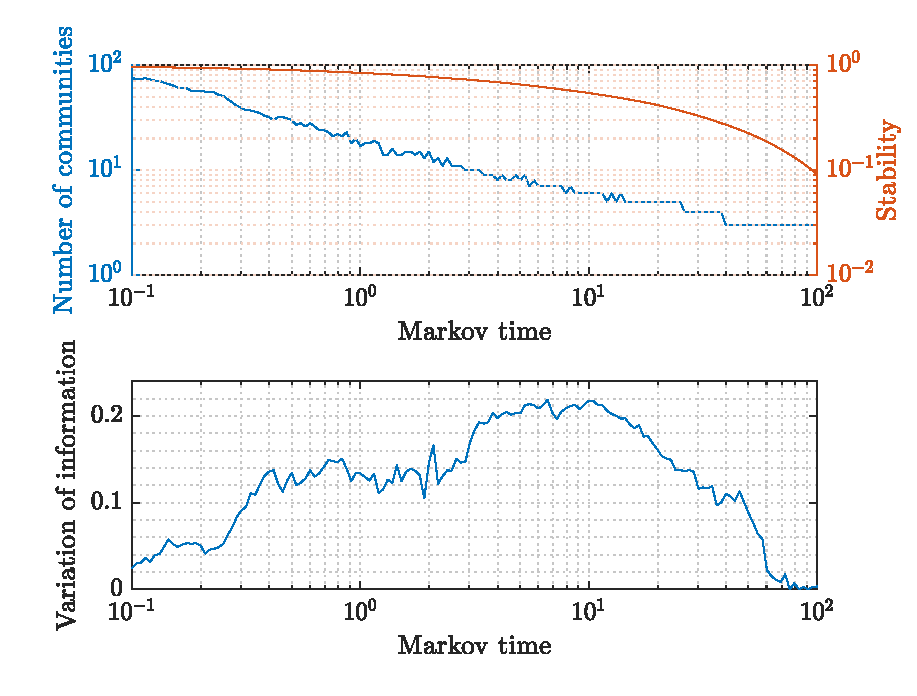
\includegraphics[width = .7\textwidth]{clusters/stab0.eps}
	\caption{Stability, number of communities and variation of information as a function of the Markov time for $T=1$ year.}
	\label{fig:stab0}
\end{figure}

\begin{figure}[H]
	\centering
	\begin{subfigure}[t]{0.49\textwidth}
		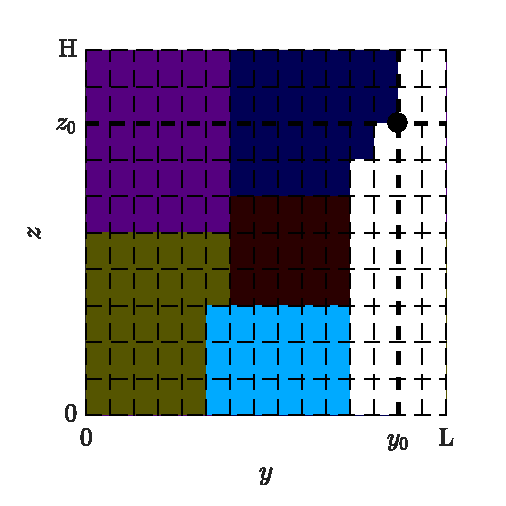
\includegraphics[width=\textwidth]{clusters/cluster0_6_.eps}
		\caption{6 communities.}
		\label{fig:cluster0_6_}
	\end{subfigure}
	\begin{subfigure}[t]{0.49\textwidth}
		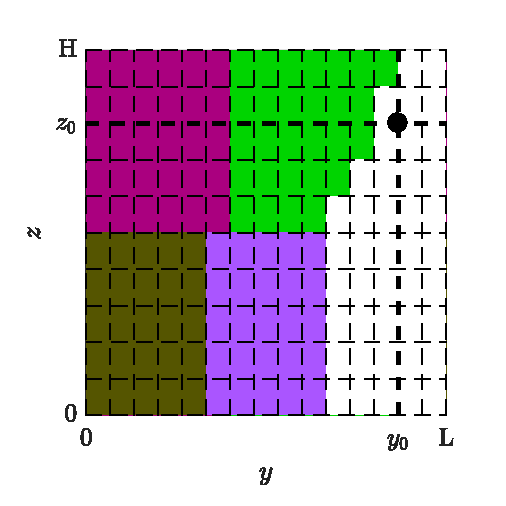
\includegraphics[width=\textwidth]{clusters/cluster0_5_.eps}
		\caption{5 communities.}
		\label{fig:cluster0_5_}
	\end{subfigure}
	\begin{subfigure}[t]{0.49\textwidth}
		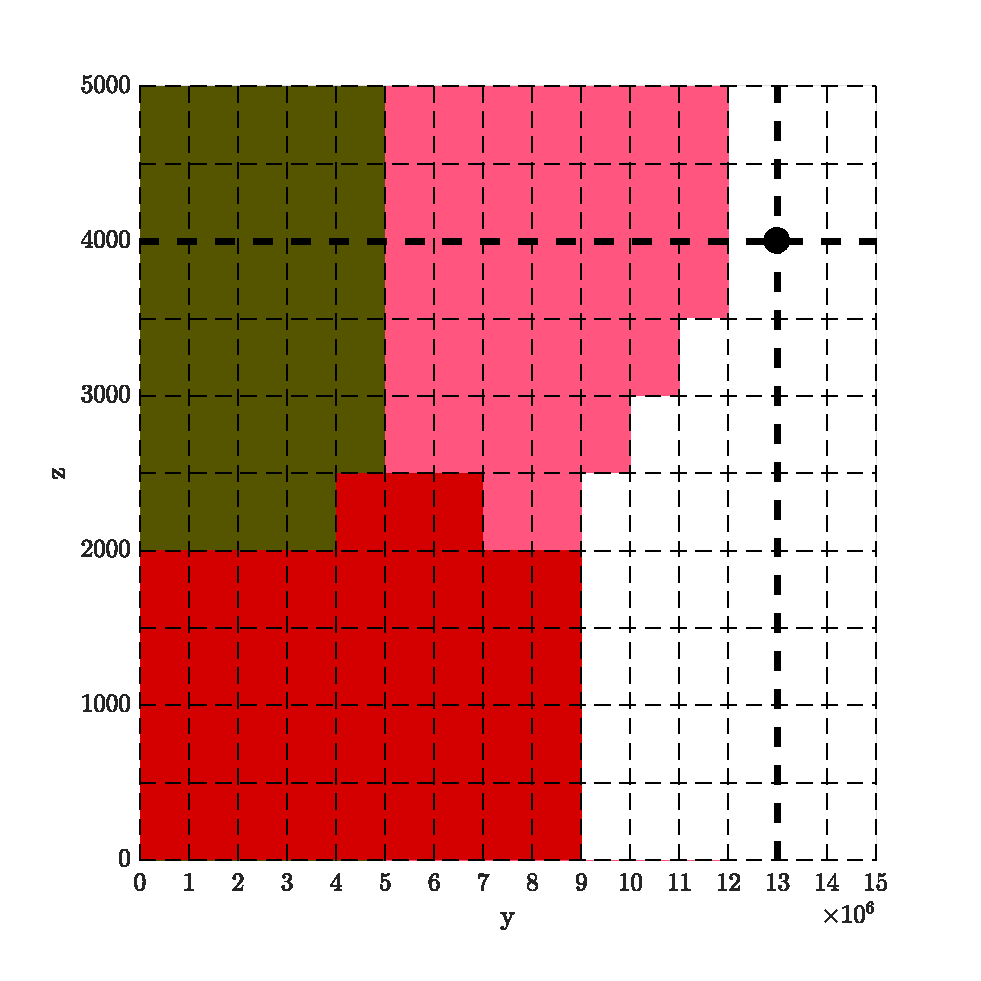
\includegraphics[width=\textwidth]{clusters/cluster0_4_.eps}
		\caption{4 communities.}
		\label{fig:cluster0_4_}
	\end{subfigure}
	\begin{subfigure}[t]{0.49\textwidth}
		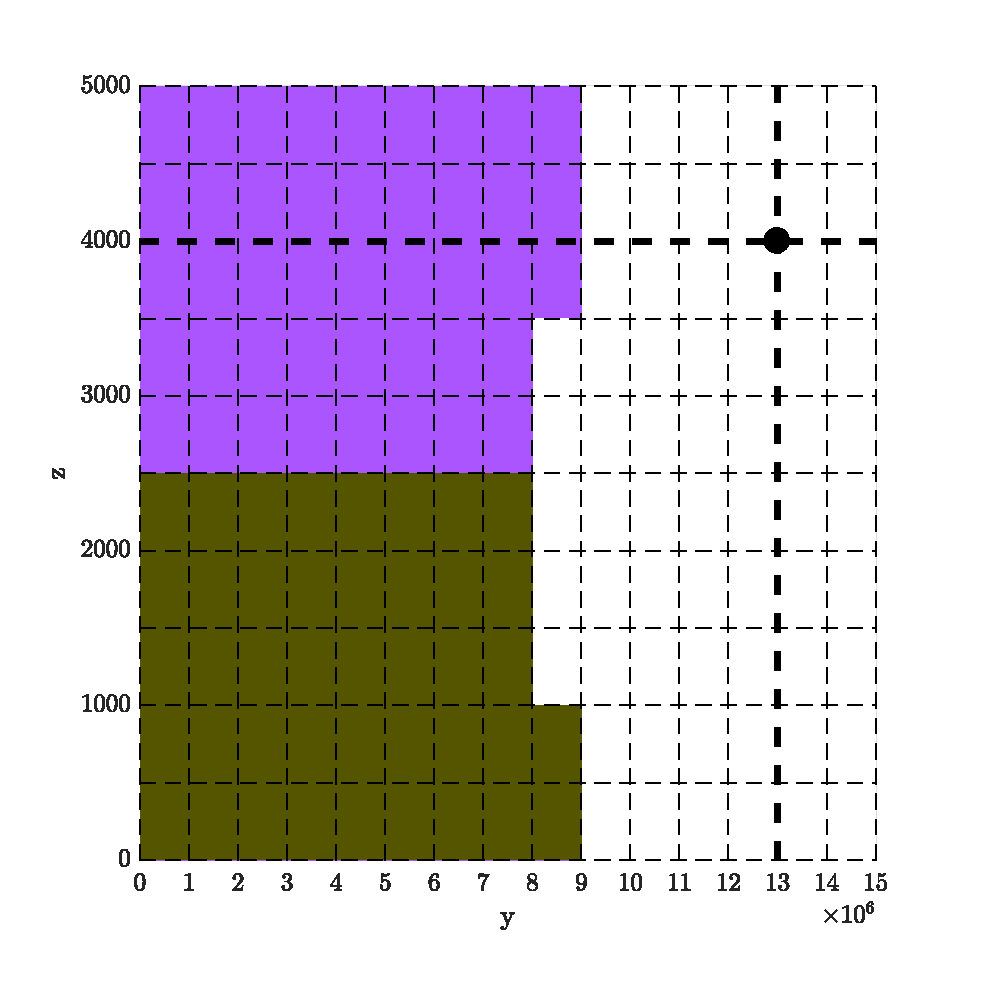
\includegraphics[width=\textwidth]{clusters/cluster0_3_.eps}
		\caption{3 communities.}
		\label{fig:cluster0_3_}
	\end{subfigure}
	\caption{The relevant clusterings detected at different time scales for $T=1$ year.}
	\label{fig:cluster0}
\end{figure}

%------------------ T = 10 -----------------------------%

\begin{figure}[H]
	\centering
	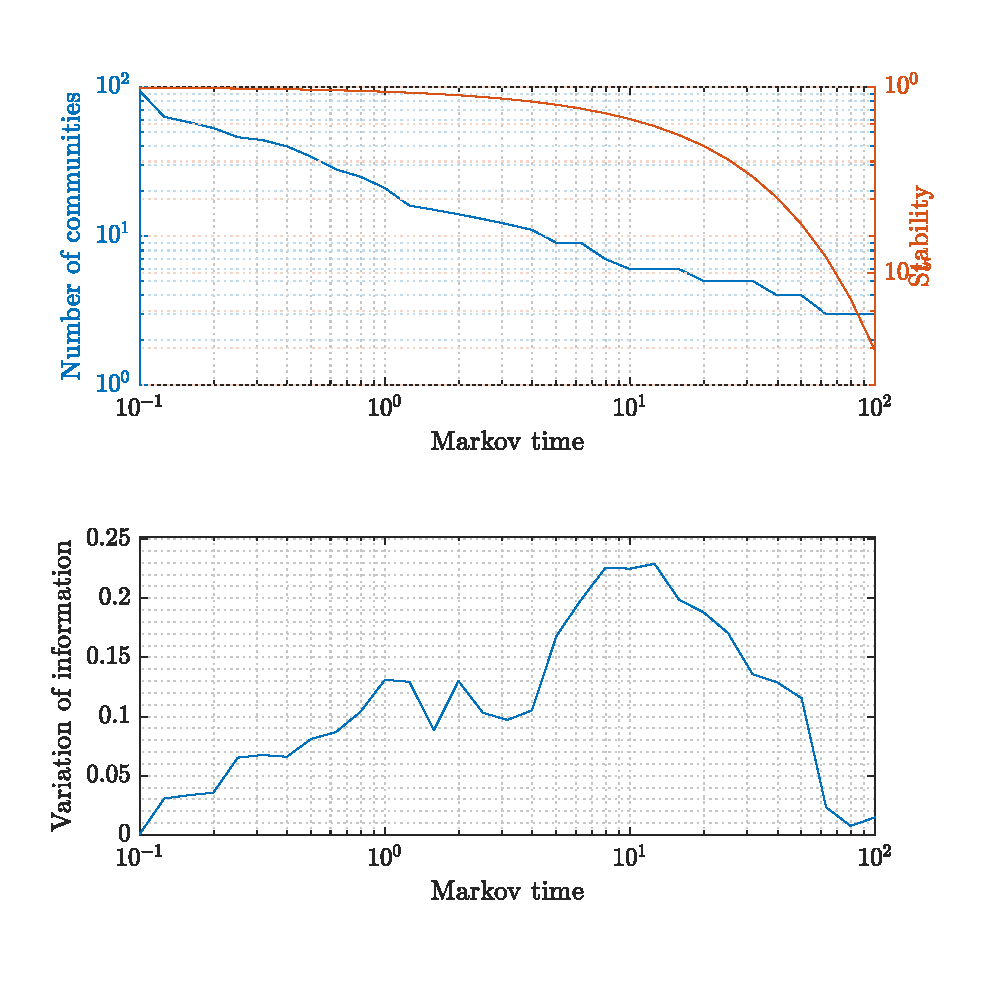
\includegraphics[width = .7\textwidth]{clusters/stab1.eps}
	\caption{Stability, number of communities and variation of information as a function of the Markov time for $T=10$ years.}
	\label{fig:stab1}
\end{figure}

\begin{figure}[H]
	\centering
	\begin{subfigure}[t]{0.49\textwidth}
		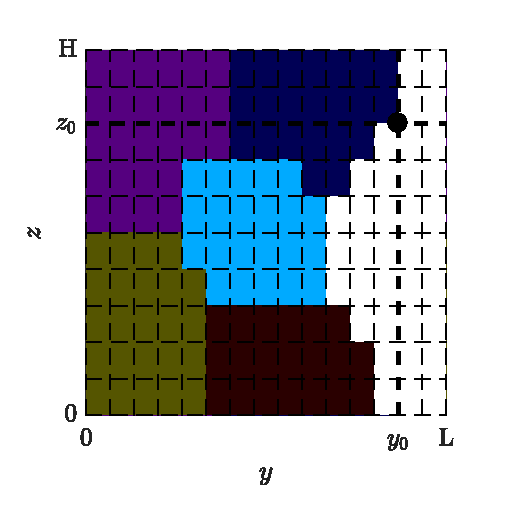
\includegraphics[width=\textwidth]{clusters/cluster1_6_.eps}
		\caption{6 communities.}
		\label{fig:cluster1_6_}
	\end{subfigure}
	\begin{subfigure}[t]{0.49\textwidth}
		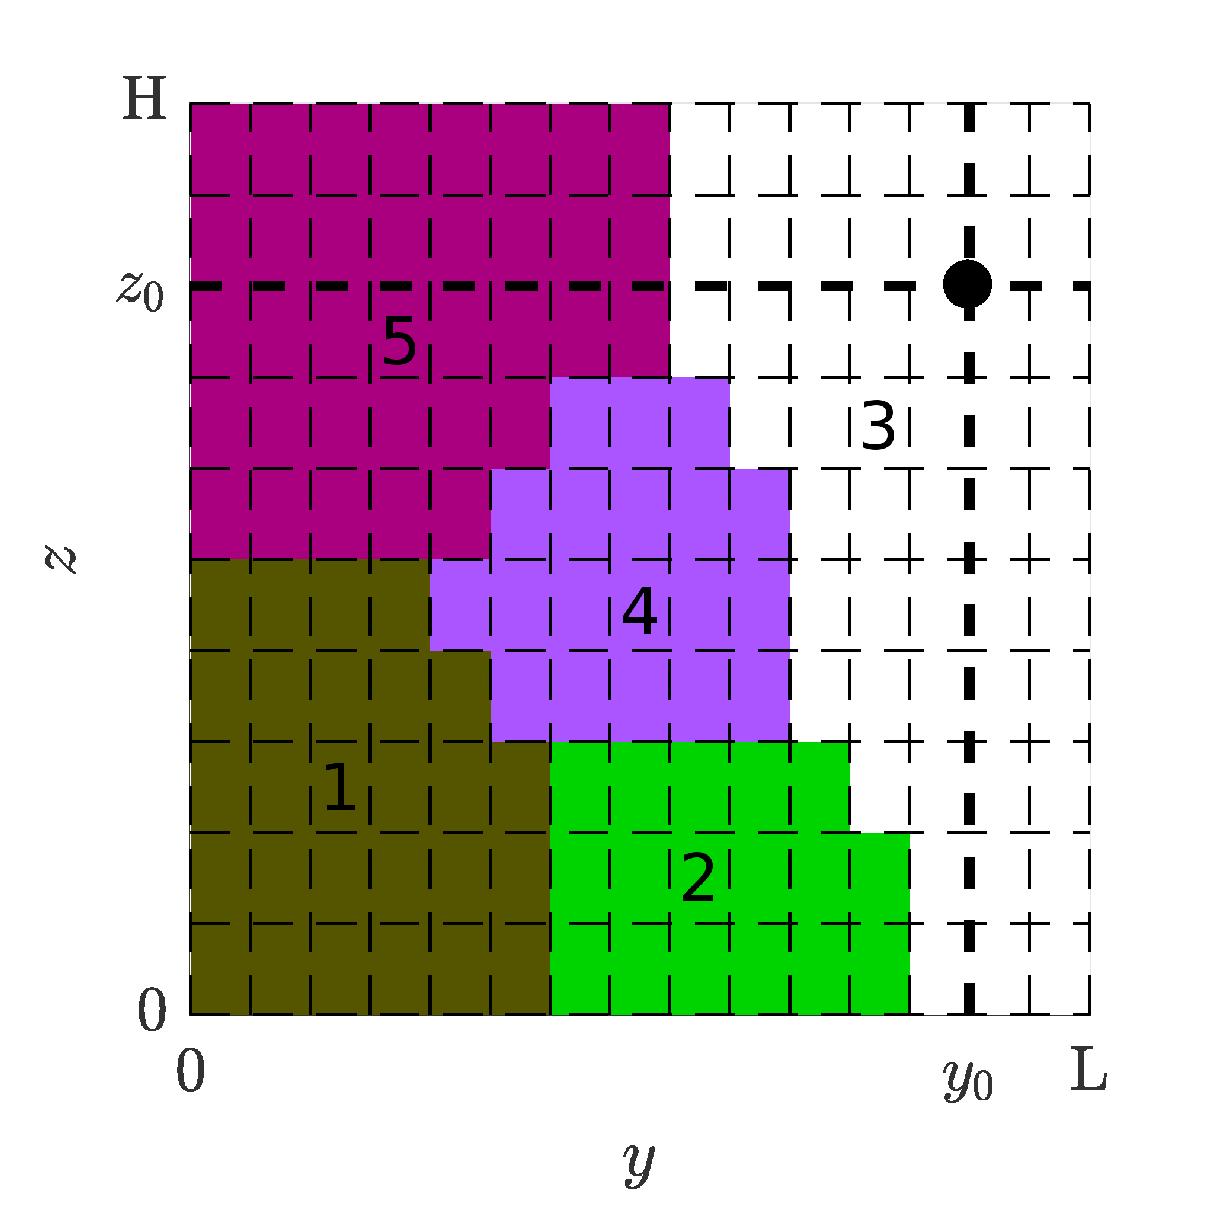
\includegraphics[width=\textwidth]{clusters/cluster1_5_num.eps}
		\caption{5 communities.}
		\label{fig:cluster1_5_}
	\end{subfigure}
	\begin{subfigure}[t]{0.49\textwidth}
		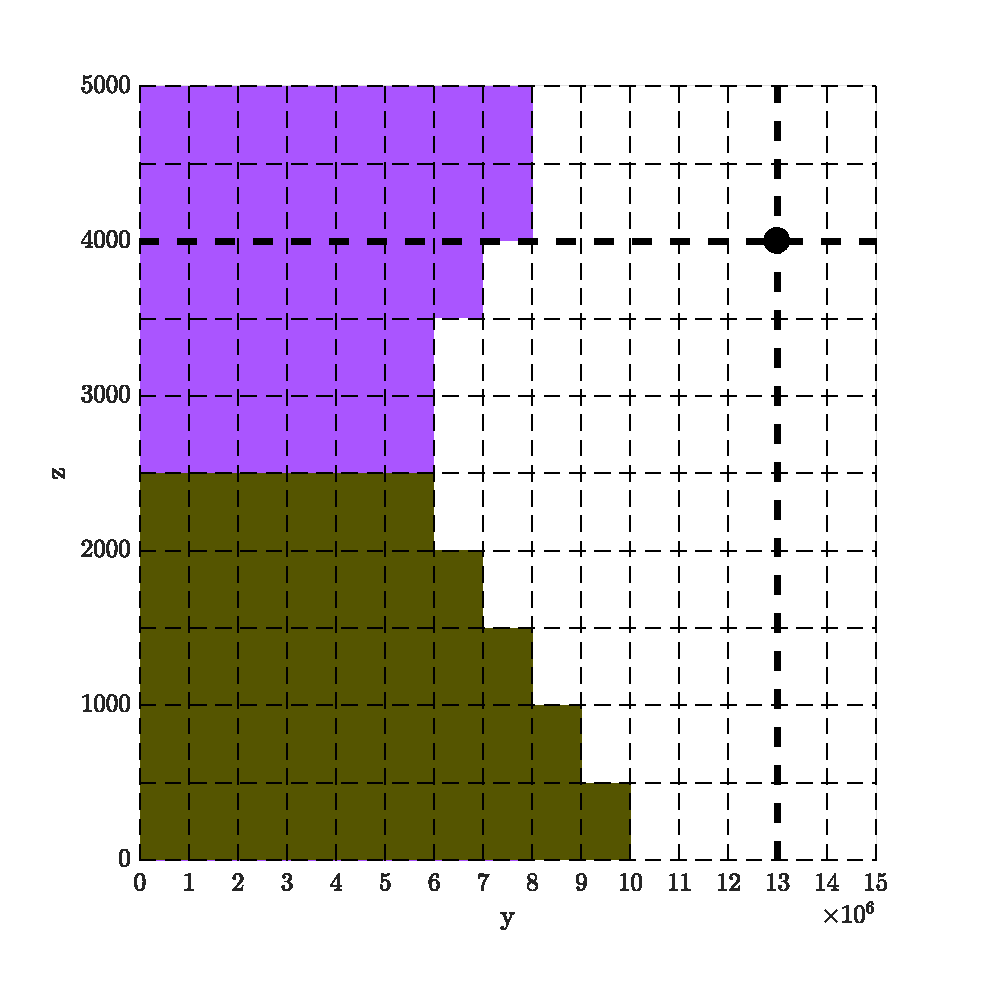
\includegraphics[width=\textwidth]{clusters/cluster1_3_.eps}
		\caption{3 communities.}
		\label{fig:cluster1_3_}
	\end{subfigure}
	\begin{subfigure}[t]{0.49\textwidth}
		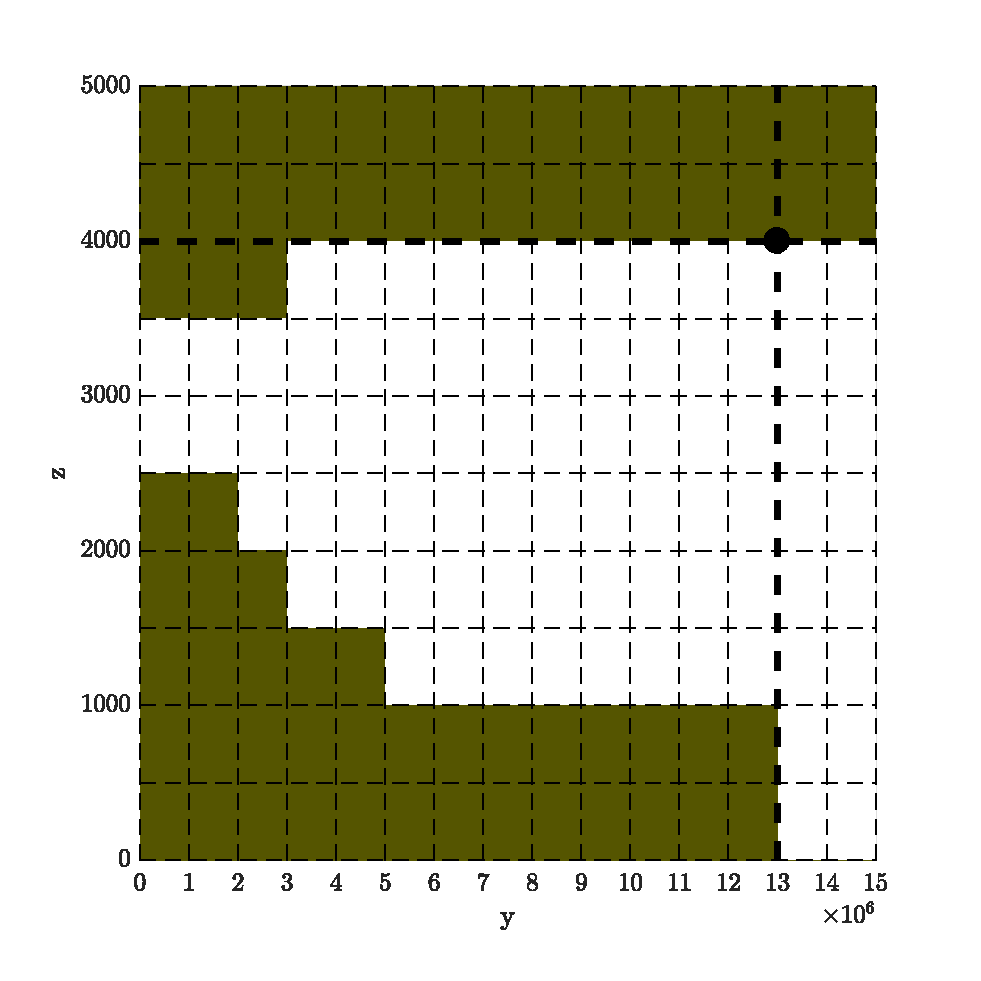
\includegraphics[width=\textwidth]{clusters/cluster1_2_.eps}
		\caption{2 communities detected by the algorithm which should rather be considered as being 3 communities.}
		\label{fig:cluster1_2_}
	\end{subfigure}
	\caption{The relevant clusterings detected at different time scales for $T=10$ years.}
	\label{fig:cluster1}
\end{figure}

%------------------ T = 50 -----------------------------%
\begin{figure}[H]
	\centering
	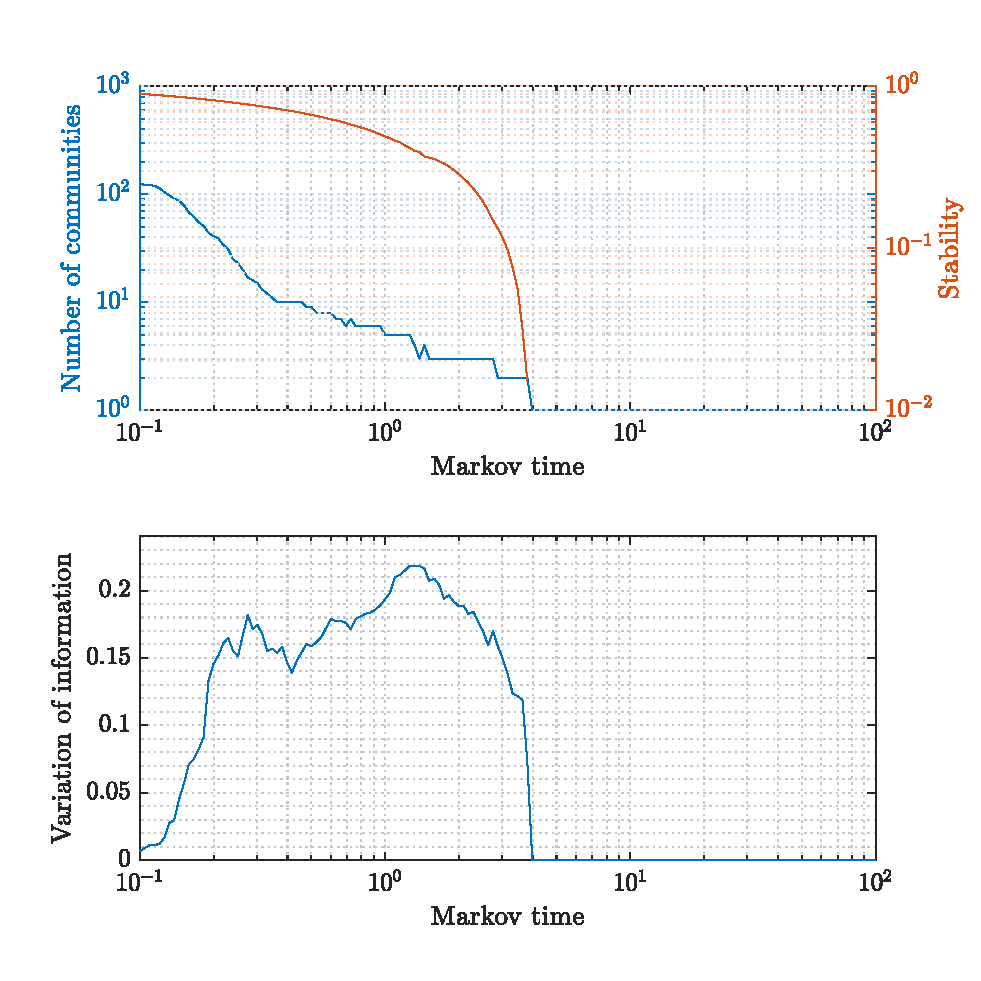
\includegraphics[width = .7\textwidth]{clusters/stab5.eps}
	\caption{Stability, number of communities and variation of information as a function of the Markov time for $T=50$ years.}
	\label{fig:stab5}
\end{figure}

\begin{figure}[H]
	\centering
	\begin{subfigure}[t]{0.49\textwidth}
		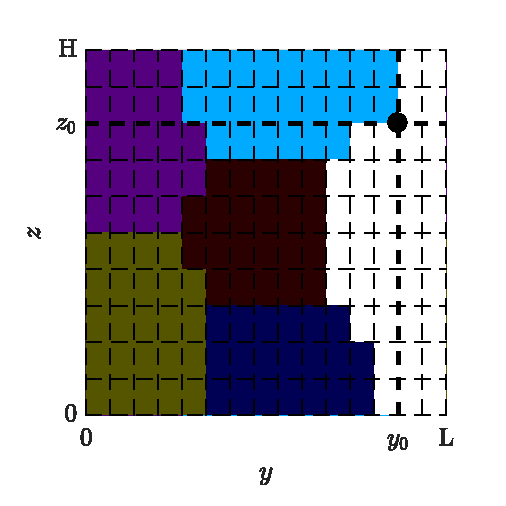
\includegraphics[width=\textwidth]{clusters/cluster5_6_.eps}
		\caption{6 communities.}
		\label{fig:cluster5_6_}
	\end{subfigure}
	\begin{subfigure}[t]{0.49\textwidth}
		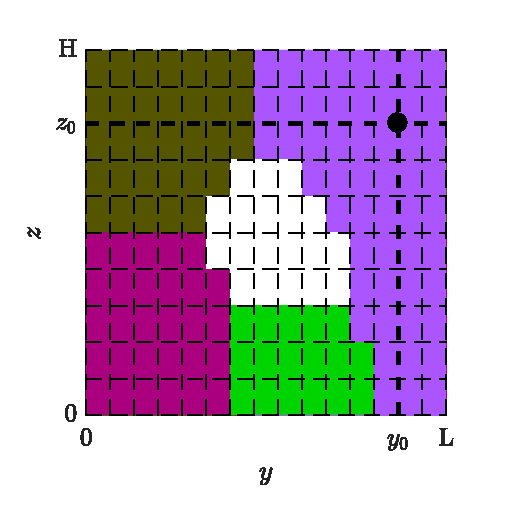
\includegraphics[width=\textwidth]{clusters/cluster5_5_.eps}
		\caption{5 communities.}
		\label{fig:cluster5_5_}
	\end{subfigure}
	\begin{subfigure}[t]{0.49\textwidth}
		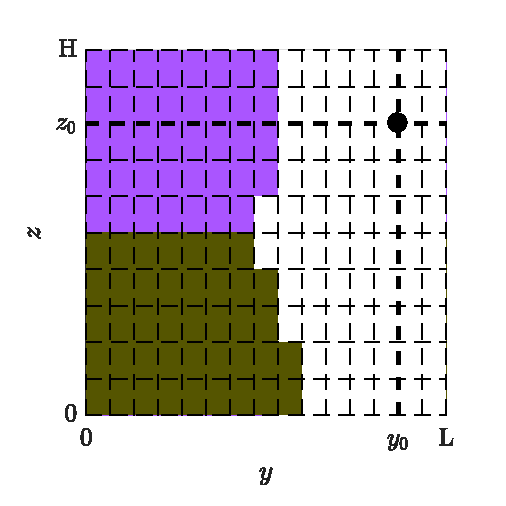
\includegraphics[width=\textwidth]{clusters/cluster5_3_.eps}
		\caption{3 communities.}
		\label{fig:cluster5_3_}
	\end{subfigure}
	\begin{subfigure}[t]{0.49\textwidth}
		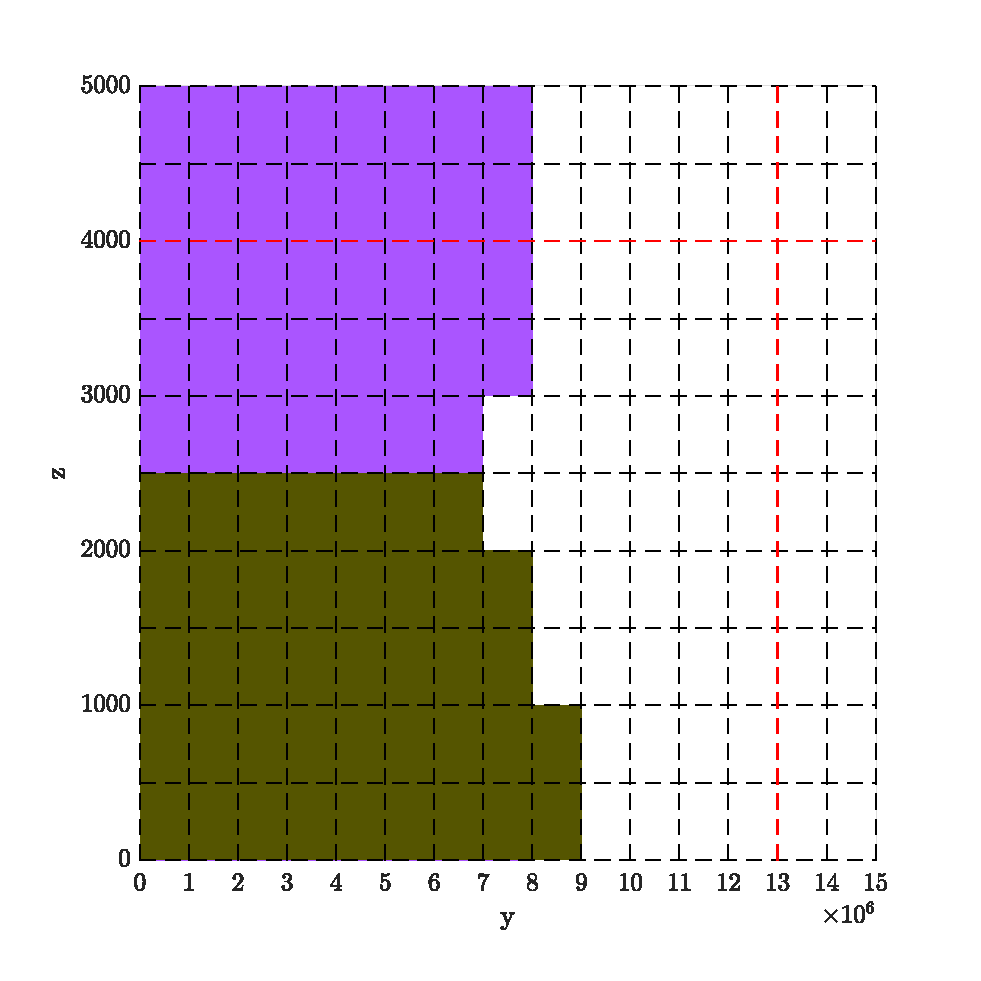
\includegraphics[width=\textwidth]{clusters/cluster5_2_.eps}
		\caption{2 communities.}
		\label{fig:cluster5_2_}
	\end{subfigure}
	\caption{The relevant clusterings detected at different time scales for $T=50$ years.}
	\label{fig:cluster5}
\end{figure}

%------------------ T = 100 ----------------------------%
\begin{figure}[H]
	\centering
	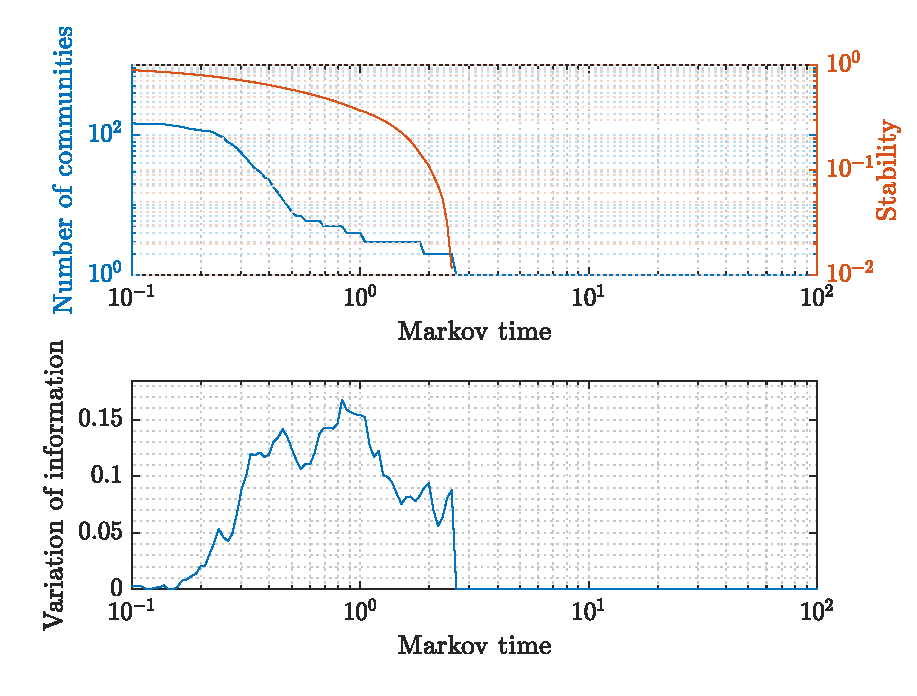
\includegraphics[width = .7\textwidth]{clusters/stab10.eps}
	\caption{Stability, number of communities and variation of information as a function of the Markov time for $T=100$ years.}
	\label{fig:stab10}
\end{figure}

\begin{figure}[H]
	\centering
	\begin{subfigure}[t]{0.49\textwidth}
		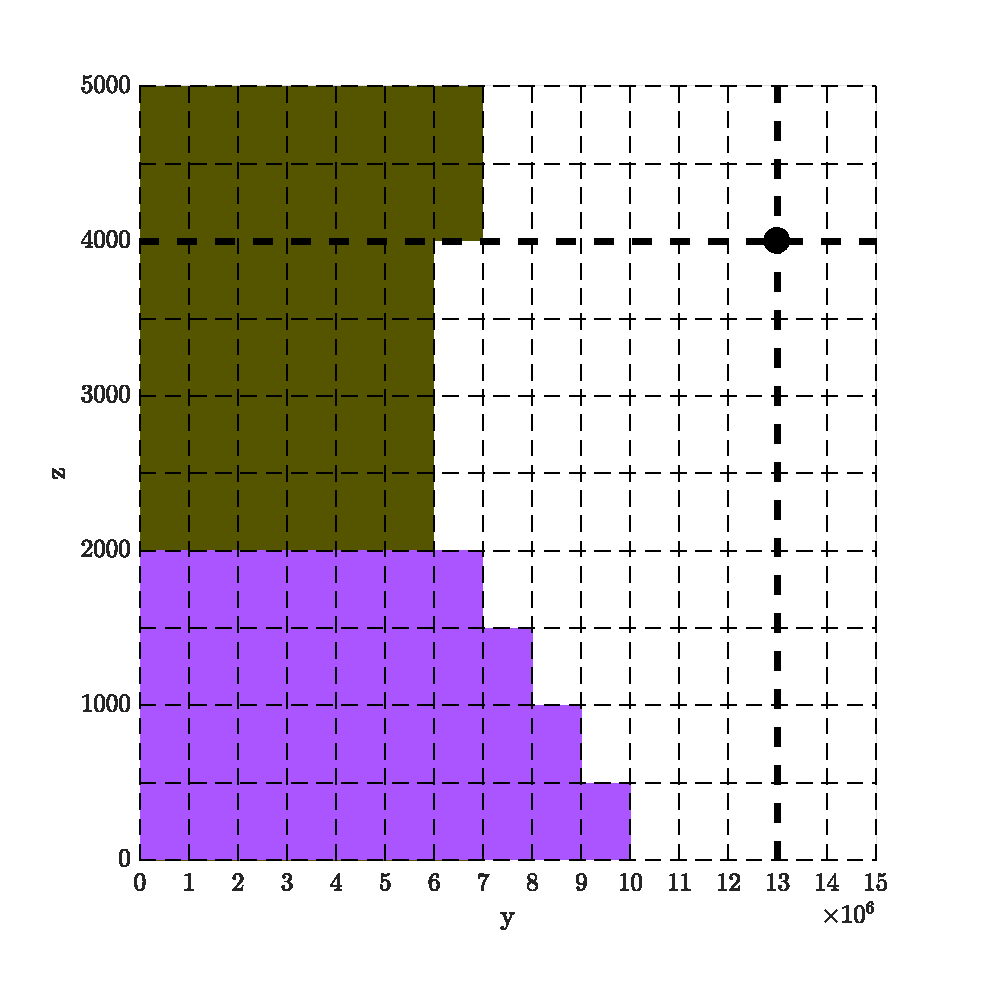
\includegraphics[width=\textwidth]{clusters/cluster10_3_.eps}
		\caption{3 communities.}
		\label{fig:cluster10_3_}
	\end{subfigure}
	\begin{subfigure}[t]{0.49\textwidth}
		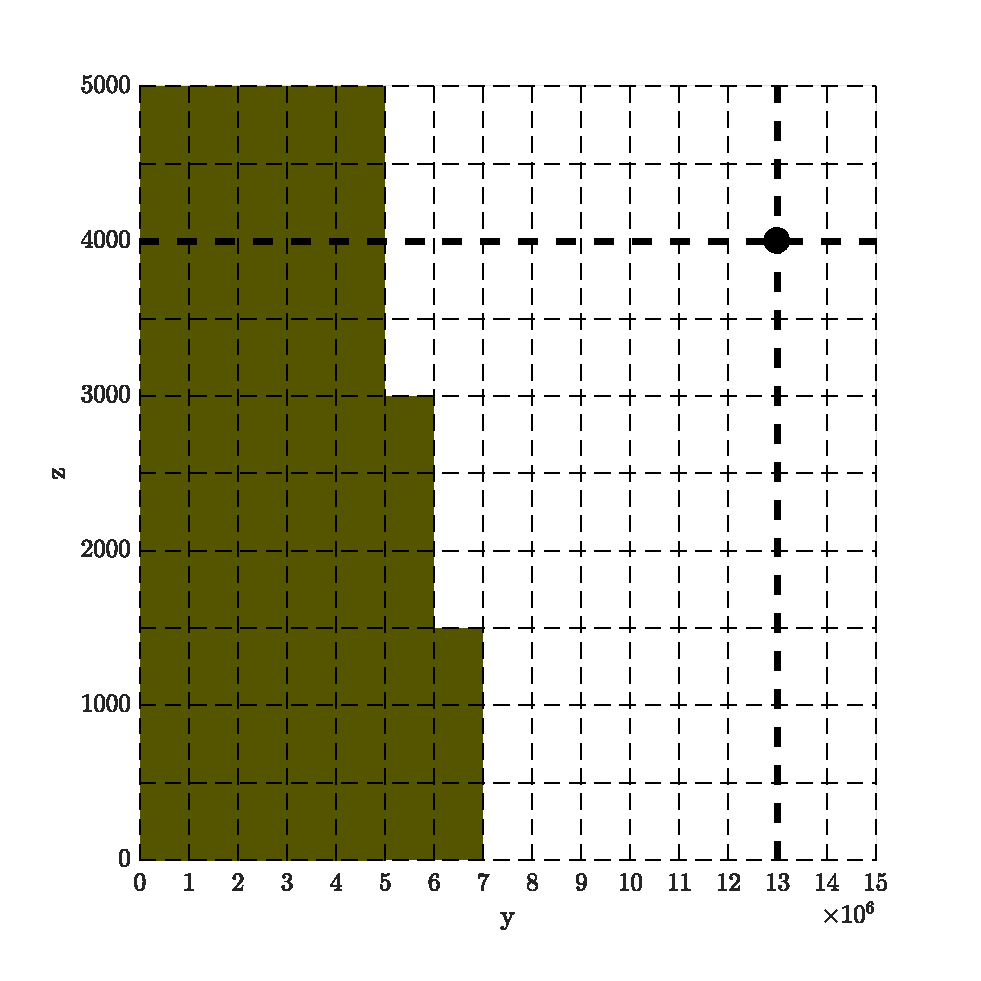
\includegraphics[width=\textwidth]{clusters/cluster10_2_.eps}
		\caption{2 communities.}
		\label{fig:cluster10_2_}
	\end{subfigure}
	\caption{The relevant clusterings detected at different time scales for $T=100$ years.}
	\label{fig:cluster10}
\end{figure}
%!TEX root = /home/renaud/Documents/EPL/tfe/latex/tfe.tex
\chapter{The transport model}
\section{The reactive transport equation}
The evolution of the concentration of a particular constituent (or tracer) in an aquatic environment is described by the \textit{reactive transport equation}:
\begin{equation}\label{eq:ADR}
	\frac{\partial C}{\partial t} = q-\nabla \cdot \left(\b uC - \b K \nabla C\right).
\end{equation}
In this equation, $C$ is the concentration of the constituent in water, expressed in $\rm{kg/m^d}$, where $d$ is the dimension of the problem; $t$ is the time, expressed in seconds; $q$ is the local net production (i.e. production - destruction) rate of the constituent, expressed in $\rm{kg/(m^ds)}$; $\b u$ is the velocity vector whose units are $\rm{m/s}$; and $\b K$ is the \textit{diffusivity tensor}, expressed in $\rm{m^2/s}$. Without loss of generality, we can assume $\b K$ to be symmetric. This is essentially because the impact of the anti-symmetric part of $\b K$, if any, may be viewed as additional advection. More details may be found in appendix A of \cite{deleersnijder2001concept}. Of course, the symmetric tensor $\b K$ must then be positive-definite in order to represent truly diffusive processes, namely phenoma which tend, at any time and location, to homogenize the concentration of any constituent.

In equation \eqref{eq:ADR}, $\nabla \cdot \b u C$ is the \textit{advective} term, $\nabla \cdot (\b K \nabla C)$ is the \textit{diffusive} term, and $q$ is often called the \textit{source/sink} term. When $q=0$, equation becomes the \textit{advection-diffusion} equation:
\begin{equation}\label{eq:C_PDE_vec}
 	\frac{\partial C}{\partial t} = -\nabla \cdot \left(\b uC - \b K \nabla C\right).
 \end{equation}
 When $q=0$, the tracer is said to be \textit{passive}.

This equation is omnipresent in this work for several reasons. It is fundamental in our purpose to develop consistent compartment models, as we will see in chapter \ref{chap:compartment}. Furthermore, we have seen in chapter \ref{chap:clustering} that the stability method is based on the knowledge of the \textit{transition probability matrix}. Computing that matrix in the case of marine models cannot be done unless we understand the dynamics of the flow: we will see in chapter \ref{chap:numerical} that efficient numerical methods allowing to track the fate of individual tracer's particles can be devised from equation \eqref{eq:ADR}. The transition probability matrix can then easily be approximated from the particles trajectories. Finally, the particles trajectories can also be used to evaluate the concentration, and hence to assess the validity of the compartment models that will be developed further in this work.

\section{The velocity field}
In general, the velocity field in equation \eqref{eq:ADR} is unknown and has to be solved from the Navier-Stokes equations. In this work, we will restrict ourselves to problems where the velocity field is known and stationary. The \textit{continuity equation} (local mass conservation)
\begin{equation} \label{eq:continuity}
	\frac{\partial \rho}{\partial t} + \nabla \cdot (\rho \b u) = 0
\end{equation}
must be satisfied everywhere on the domain. In equation \eqref{eq:continuity}, $\rho$ is the density of the seawater mixture. In order to simplify the continuity equation, we make the very common \textit{Boussinesq approximation}. In the aquatic environment, water is, by far, the dominant constituent. The density of seawater is thus close to that of pure water, $\rho_w$. The latter depends on the temperature and pressure, but the variations are often very small: this consideration is at the basis of the Boussinesq approximation. Let $\bar{\rho}$ and $\Delta\rho$ be appropriate reference values of the density and the order of magnitude of its variation. The key assumption in the \textit{Boussinesq approximation} is that
\begin{equation} \label{eq:bouss_hyp}
	\frac{\Delta \rho}{\bar{\rho}} \ll 1.
\end{equation}
To assess the impact of this assumption on the continuity equation, we consider its dimensionless form. Let $U$, $T$ and $X$ be relevant velocity-, time- and space-scales. This allows to introduce the following dimensionless variables (denoted by primes):
\begin{equation}
	\rho' = \frac{\rho - \bar{\rho}}{\Delta \rho}, \quad \b u' = \frac{\b u}{U}, \quad t' = \frac{t}{T}, \quad \mbox{and} \quad \b x' = \frac{\b x}{X},
\end{equation}
where $\b x = (y,z)$. The dimensionless version of the continuity equation \eqref{eq:continuity} reads then: 
\begin{equation}
	\frac{\Delta \rho}{T}\frac{\partial \rho'}{\partial t'} + \frac{U\Delta \rho}{X}\b u' \cdot \nabla' \rho' + \frac{U(\bar{\rho}+ \rho' \Delta \rho)}{X}\nabla' \cdot \b u' = 0.
\end{equation}
Multiplying both sides by $X/(U\bar{\rho})$ yields :
\begin{equation}
	\frac{X}{UT}\frac{\Delta \rho}{\bar{\rho}}\frac{\partial \rho'}{\partial t'} + \frac{\Delta \rho}{\bar{\rho}}\b u' \cdot \nabla' \rho' + \left(1+\frac{\Delta \rho}{\bar{\rho}}\rho'\right)\nabla' \cdot \b u' = 0.
\end{equation}
By taking \eqref{eq:bouss_hyp} into account, this equation simplifies to $\nabla' \cdot \b u' = 0$, or equivalently in dimensional variables 
\begin{equation}
	\nabla \cdot \b u = 0.
\end{equation}

\section{Properties of the solution of the advection-diffusion equation}
In this section, we show the most important properties related to the advection-diffusion equation. To this end, let us first introduce some notations and terminology. Let $\Omega$ denote the (time independent) domain of interest and $\partial \Omega$ its boundary. The outward unit normal vector to $\partial \Omega$ is denoted $\hat{\b n}$. The volume of the domain is
\begin{equation}
	V = \int_{\Omega} \rm d\Omega.	
\end{equation}
An \textit{isolated} domain is such that there is no exchange with the environment, and hence no net flux of the fluid crossing the boundary:
\begin{equation} \label{eq:isolateddomain}
	\left. \b u \cdot \hat{\b n}\right|_{\b x \in \partial \Omega} = 0.
\end{equation}

\begin{property} \label{prop:mass-is-constant}
	If the domain is isolated and the tracer is passive, the tracer mass contained in the domain of interest is a constant.
\end{property}
\begin{proof}
	Since the domain is isolated, the tracer flux crossing the boundary must be zero:
	\begin{equation} \label{eq:isolateddomain2}
		\left. (C\b u - \b K \nabla C)\cdot \n \right|_{\b x \in \partial \Omega} = 0.
	\end{equation}
	This equation combined to equation \eqref{eq:isolateddomain} implies that
	\begin{equation} \label{eq:isolateddomain3}
		\left. (C\b u)\cdot \n \right|_{\b x \in \partial \Omega} = 0 \quad \mbox{and} \quad \left. (- \b K \nabla C)\cdot \n \right|_{\b x \in \partial \Omega} = 0.
	\end{equation}
	The total mass of tracer in the domain is
	\begin{equation}
		m(t) = \int_{\Omega} C(\b x,t) \rm d\Omega,
	\end{equation}
	and its time derivative
	\begin{equation} \label{eq:tracermass1}
		\frac{dm(t)}{dt} = \frac{d}{dt} \int_{\Omega} C(\b x,t) \rm d\Omega = \int_{\Omega} \frac{\partial}{\partial t} C(\b x,t) \rm d\Omega.
	\end{equation}
	Injecting \eqref{eq:C_PDE_vec} into \eqref{eq:tracermass1} leads to
	\begin{equation}
		\frac{dm(t)}{dt} = \int_{\Omega} -\nabla \cdot \left(\b uC - \b K \nabla C\right) \rm d\Omega = \int_{\partial \Omega} -\left(\b uC - \b K \nabla C\right) \cdot \n \ \rm d(\partial \Omega)
	\end{equation}
	where we have used the divergence theorem. Finally, by \eqref{eq:isolateddomain2} this last expression is equal to zero, which concludes the proof.
\end{proof}

\begin{property}
	For a passive tracer in an isolated domain, the variance of the concentration decreases monotonously with time until the concentration is everywhere equal to the mean concentration. In other words, the tracer concentration gets more and more homogeneous with time until the equilibrium state is reached, namely when the concentration is constant and uniform everywhere on $\Omega$.
\end{property}
\begin{proof}
	By property \ref{prop:mass-is-constant}, the total mass of tracer is constant. Hence, the mean concentration over $\Omega$, $\bar C$, is also constant:
	\begin{equation}
	 	\bar C = \frac{1}{V} \int_{\Omega} C(\b x,t) \rm d\Omega = \frac{m}{V}.
	 \end{equation} 
	 Let $\hat C(\b x,t) := C(\b x,t) - \bar C$ denote the deviation of the concentration with respect to $\bar C$. The variance of the concentration is
	 \begin{equation}
	 	\sigma^2(t) = \frac{1}{V} \int_{\Omega} \left(\hat C(\b x,t)\right)^2 \rm d\Omega.
	 \end{equation}
	 This quantity is a measure of the concentration inhomogeneity. Notice that $\bar C$ satisfies the advection diffusion equation:
	 \begin{equation}
	 	0 = \frac{\partial \bar C}{\partial t} = -\nabla \cdot \left(\b u \bar C - \b K \nabla \bar C\right) = - \bar C \nabla \cdot (\b u - 0) = 0,
	 \end{equation}
	 and thus
	 \begin{equation} \label{prop:variance1}
	 	\frac{\partial \hat C}{\partial t} = -\nabla \cdot \left(\b u \hat C - \b K \nabla \hat C\right).
	 \end{equation}
	 Multiplying equation \eqref{prop:variance1} by $\hat C$ yields, after some calculations
	 \begin{equation} \label{prop:variance2}
	 	\frac{\partial \hat C^2}{\partial t} = - \nabla \cdot \left(\hat C^2 \b u \right) + 2\nabla \cdot \left(\hat C \b K \nabla \hat C \right) - 2 \nabla \hat C^\t \b K \nabla \hat C.
	 \end{equation}
	 Now, notice that
	 \begin{equation} \label{prop:variance3}
	 	\int_{\Omega} \frac{\partial \hat C^2}{\partial t} \rm d\Omega = \frac{d}{dt} \int_{\Omega} \left( \hat C(\b x,t) \right)^2 \rm d\Omega = V\frac{d\sigma^2}{dt}.
	 \end{equation}
	 Combining \eqref{prop:variance2} and \eqref{prop:variance3} yields
	 \begin{equation}
	 	V\frac{d\sigma^2}{dt} = - \int_{\Omega} \nabla \cdot \left(\hat C^2 \b u \right) \rm d\Omega + 2 \int_{\Omega} \nabla \cdot \left(\hat C \b K \nabla \hat C \right) \rm d\Omega -2 \int_{\Omega} \nabla \hat C^\t \b K \nabla \hat C \rm d\Omega.
	 \end{equation}
	 Using the divergence theorem and equations \eqref{eq:isolateddomain} and \eqref{eq:isolateddomain3}, we get
	 \begin{equation}
	 		V\frac{d\sigma^2}{dt} = - \underbrace{\int_{\partial \Omega} \hat C^2 (\b u \cdot \n) \rm d(\partial \Omega)}_{=0} + 2\underbrace{\int_{\partial \Omega} \hat C^ (\b K \nabla \hat C \cdot \n) \rm d(\partial \Omega)}_{=0} -2 \int_{\Omega} \nabla \hat C^\t \b K \nabla \hat C \rm d\Omega.
	 \end{equation}
	 Finally,
	 \begin{equation}
	 	\frac{d\sigma^2}{dt} = -\frac{2}{V} \int_{\Omega} \nabla \hat C^\t \b K \nabla \hat C \rm d\Omega.
	 \end{equation}
	 Since $\b K$ is positive definite, the variance of the concentration will decrease until $\nabla \hat C = 0$, hence until $C$ reaches a constant value everywhere on $\Omega$. The only possibility is $\bar C$, and thus we have shown that
	 \begin{equation}
	 	\lim_{t\rightarrow \infty} C(\b x,t) = \bar C.
	 \end{equation}
\end{proof}
%!TEX root = /home/renaud/Documents/EPL/tfe/latex/tfe.tex
\chapter{Structure of a compartment model for tracer transport} \label{chap:compartment}
% The previous chapters cover the material needed to derive compartments from the dynamics of a tracer transport model. But deciding which subdomains define the compartments is only the first step in building a compartment model. 
A relevant compartment model should reproduce the properties covered in section~\ref{sec:propcontinuous} for the corresponding continuous model. In this chapter, a compartment model structure that fulfills that requirement is proposed, and the corresponding matrix form is derived. This chapter is widely inspired from \cite{deleersnijder2014compartment} and \cite{delhez2010compartment}.

%!TEX root = /home/renaud/Documents/EPL/tfe/latex/tfe.tex
\section{Formulation of a compartment model} \label{sec:fcm}
Recall that the evolution of the concentration $C(t,\b x)$ of a tracer in a domain $\Omega$ obeys the following equation:
\begin{equation} \label{eq:continuousproblem}
	\frac{\partial C}{\partial t} = q - \nabla \cdot (\b u C - \b K \cdot \nabla C),
\end{equation}
where $\b u$ is the velocity field and $q$ is the source or sink term, i.e. the rate at which the tracer is produced or destroyed. In the case of a passive tracer, $q = 0$. Under the Boussinesq approximation, the continuity equation simplifies to
\begin{equation}
	\nabla \cdot \b u = 0,
\end{equation}
namely the velocity field is divergence-free. As already stated, the diffusivity tensor $\b K$ is symmetric and positive definite.

In order to derive a compartment model from \eqref{eq:continuousproblem}, $\Omega$ must be partitioned into $N$ subdomains $\Omega_i$ ($i = 1,\dots,N$) called the \textit{compartments}. The interface between the subdomains $\Omega_i$ and $\Omega_j$ is denoted $\Gamma_{i,j}$ and the interface between $\Omega_i$ and the environment is denoted $\Gamma_{i,e}$. Obviously, $\Gamma_{i,j} = \Gamma_{j,i}$. In a compartment model, only the averages over the compartments are considered. The mean tracer concentration over compartment $i$ is 
\begin{equation}
	C_i(t) = \frac{1}{\Omega_i} \int_{\Omega_i} C(t,\b x) \rm d\Omega_i,
\end{equation}
and the production/destruction term over the subdomain $i$ becomes
\begin{equation}
	q_i(t) =  \frac{1}{\Omega_i} \int_{\Omega_i} q(t,\b x) \rm d\Omega_i.
\end{equation}
The equation governing the evolution of $C_i(t)$, the average concentration in compartment $i$, is obtained by integrating \eqref{eq:continuousproblem} over $\Omega_i$. This yields, using Gauss's Theorem:
\begin{equation}
	\Omega_i \frac{d C_i}{d t} = \Omega_i q_i - \sum_{\subalign{j&=1 \\j &\neq i}}^N \underbrace{\int_{\Gamma_{i,j}} (\b u C - \b K \cdot \nabla C)\cdot \b n_{i,j} \rm d\Gamma_{i,j}}_{\phi_{i,j}} - \underbrace{\int_{\Gamma_{i,e}} (\b u C - \b K \cdot \nabla C)\cdot \b n_{i,e} \rm d\Gamma_{i,e}}_{\phi_{i,e}}.
\end{equation}
In the framework of a compartment model, only the mean concentration in each compartment are available, making it impossible to evaluate the integrals in the right-hand side exactly. The flux $\phi_{i,j}$ can be split into an advective and a diffusive part:
\begin{equation} \label{eq:phi_i,j}
	\phi_{i,j} = \underbrace{\int_{\Gamma_{i,j}} (\b u C)\cdot \b n_{i,j} \rm d\Gamma_{i,j}}_{:= \phi_{i,j}^A \mbox{ \footnotesize (advective part)}} + \underbrace{\int_{\Gamma_{i,j}} (-\b K \cdot \nabla C)\cdot \b n_{i,j} \rm d\Gamma_{i,j}}_{:= \phi_{i,j}^D \mbox{ \footnotesize (diffusive part)}}.
\end{equation} 
A natural approximation of the advective flux $\phi_{i,j}^A$ is obtained as
\begin{equation}
	\phi_{i,j}^A \approx \frac{C_i + C_j}{2} \int_{\Gamma_{i,j}} \b u \cdot \b n_{i,j} \rm d\Gamma_{i,j} =  \frac{C_i + C_j}{2} \Gamma_{i,j} u_{i,j},
\end{equation}
where a characteristic speed $u_{i,j}$ has been introduced such that
\begin{equation} \label{eq:def_uij}
	\Gamma_{i,j}u_{i,j} = \int_{\Gamma_{i,j}}\b u \cdot \b n_{i,j} \rm d\Gamma_{i,j}.
\end{equation}
Since $\phi_{i,j}^A = - \phi_{j,i}^A$ and $\Gamma_{i,j} = \Gamma_{j,i}$, the characteristic speed must satisfy
\begin{equation}
	u_{i,j} = - u_{j,i}.
\end{equation}
The definition \eqref{eq:def_uij} satisfies that condition.
The diffusive flux $\phi_{i,j}^D$ involves the gradient of the concentration at the interface. A possible approximation is given by
\begin{equation}
	\phi_{i,j}^D = - \Gamma_{i,j} k_{i,j} \frac{C_j-C_i}{l_{i,j}},
\end{equation}
where $k_{i,j} > 0$ is a characteristic diffusivity and $l_{i,j} > 0$ is a characteristic length. Obviously, $\phi_{i,j}^D = -\phi_{j,i}^D$ hence $k_{i,j} = k_{j,i}$ and $l_{i,j} = l_{j,i}$. In \cite{deleersnijder2014compartment}, \textit{Deleersnijder} proposes to simplify those notations by introducing advective and diffusive "fluxes" $U_{i,j}$ and $V_{i,j}$:
\begin{equation} \label{eq:def_Uij_Vij}
	U_{i,j} = \Gamma_{i,j}u_{i,j} \quad \mbox{and} \quad V_{i,j} = \frac{\Gamma_{i,j}k_{i,j}}{l_{i,j}}.
\end{equation}
By the previously mentioned properties, it is obvious that 
\begin{equation} \label{eq:Uprop}
	U_{i,j} = -U_{j,i}
\end{equation} 
and that 
\begin{equation} \label{eq:Vprop}
	V_{i,j} = V_{j,i} > 0.
\end{equation}
Using those notations, the flux from compartment $i$ to compartment $j$ is approximated by
\begin{equation}
	\phi_{i,j} \approx U_{i,j} \frac{C_i + C_j}{2} - V_{i,j}(C_j - C_i),
\end{equation}
and the equation governing the evolution of the concentration in compartment $i$ is obtained as
\begin{equation} \label{eq:compartmentmodel}
	\Omega_i \frac{dC_i}{dt} = \Omega_i q_i - \sum_{\subalign{j&=1 \\j &\neq i}}^N \left[ U_{i,j}\frac{C_i + C_j}{2} - V_{i,j} (C_j-C_i)\right] - \phi_{i,e}.
\end{equation}
Let us fix the convention $U_{i,i} = 0$ and $V_{i,i} = 0$ so that the summation subscript $j \neq i$ becomes unnecessary.
Note that by \eqref{eq:def_Uij_Vij}, \eqref{eq:def_uij} and Gauss's theorem,
\begin{equation} \label{eq:continuitycompartment}
	\sum_{\subalign{j&=1 \\j &\neq i}}^N U_{i,j} + U_{i,e} = \sum_{\subalign{j&=1 \\j &\neq i}}^N \int_{\Gamma_{i,j}}\b u \cdot \b n_{i,j} \rm d\Gamma_{i,j} + \int_{\Gamma_{i,e}}\b u \cdot \b n_{i,e} \rm d\Gamma_{i,e} = \int_{\Omega_{i}} (\nabla \cdot \b u) \rm d\Omega_{i} = 0,
\end{equation}
the counterpart to the continuity equation.
%!TEX root = /home/renaud/Documents/EPL/tfe/latex/tfe.tex
\section{Properties of the compartment model solution} \label{sec:prop_comp}
In section~\ref{sec:propcontinuous}, important properties of the continuous transport model have been derived. In this section, the counterparts of those properties are established in the case of a compartment model. The domain-averaged concentration can be expressed in terms of the compartments concentrations. Indeed, by equations \eqref{eq:Cmean} and \eqref{eq:C_i(t)}:
\begin{equation} \label{eq:Cmean_compartment}
	\bar{C}(t) = \frac{1}{|\Omega|} \int_\Omega C(\b x,t) \rm d\Omega = \frac{1}{|\Omega|} \sum_{i=1}^N \int_{\Omega_i} C(\b x,t) \rm d\Omega_i
		= \frac{1}{|\Omega|} \sum_{i=1}^N |\Omega_i| C_i(t).
\end{equation}
The variance of the concentration is approximated by the \textit{box variance}
\begin{equation}
	\sigma_{box}^2(t) = \frac{1}{|\Omega|} \sum_{i=1}^{N} |\Omega_i| \left[C_i(t) - \bar{C}(t)\right]^2.
\end{equation}

\begin{property} \label{prop1_comp}
	The mean tracer concentration $\bar C$ is not influenced by the internal advective and diffusive fluxes.
\end{property}
\begin{proof}
	By~\eqref{eq:Cmean_compartment},~\eqref{eq:compartmentmodel},~\eqref{eq:Uprop} and~\eqref{eq:Vprop}, we get successively
	\begin{subequations}
	\begin{align}
		\frac{d\bar{C}}{dt} &= \frac{1}{|\Omega|} \sum_{i=1}^N |\Omega_i| \frac{dC_i(t)}{dt}\\
			&= \frac{1}{|\Omega|} \sum_{i=1}^N \left[|\Omega_i| q_i - \sum_{j=1}^N \left[ U_{i,j}\frac{C_i + C_j}{2} - V_{i,j} (C_j-C_i)\right] - \phi_{i,e} \right]\\
			&= \frac{1}{|\Omega|} \sum_{i=1}^N(|\Omega_i| q_i + \phi_{e,i}). \label{eq:prop1deleersnijder}
	\end{align}
	\end{subequations}
\end{proof}

\begin{corollary}{prop1_comp} \label{cor:Cmeanconstant}
	For a passive tracer in an isolated domain, the mean tracer concentration within the whole domain $\bar C$ is a constant.
\end{corollary}
\begin{proof}
	The proof is straightforward by introducing $q_i = 0$ (passive tracer) and $\phi_{i,e} = 0$ (isolated domain) in equation~\eqref{eq:prop1deleersnijder}.	
\end{proof}

\begin{property} \label{prop2_comp}
	If the tracer is passive, the domain isolated and the initial concentration is constant, then the concentration stays constant.
\end{property}
\begin{proof}
	If the initial concentration is constant, then $C_i(0) = C_0$ for all $i = 1,\dots,N$. At time $t=0$, equation~\eqref{eq:compartmentmodel} becomes
	\begin{equation}
		|\Omega_i| \frac{dC_i}{dt} = -C_0 \sum_{j=1}^N U_{i,j},
	\end{equation}
	which is equal to zero by~\eqref{eq:continuitycompartment}. Here we have used that $q_i = 0$ and $\phi_{i,e} = 0$ (and thus $U_{i,e}=0$) since the tracer is passive and the domain is isolated.
\end{proof}

\begin{property} \label{prop3_comp}
	For a passive tracer ($q_i = 0$) in an isolated domain ($\phi_{i,e} = 0$), the box variance of the concentration decreases monotonically until $C_i(t) = \bar{C}(0)$ for all $i = 1,\dots,N$ (i.e., until the tracer distribution is uniform and equal to $\bar C(0)$ everywhere).
\end{property}
\begin{proof}
	Let $\hat{C}_i(t)$ denote the deviation of the concentration in compartment $i$ with respect to the mean concentration over the whole domain:
	\begin{equation}
		\hat{C}_i(t) := C_i(t) - \bar C(t).
	\end{equation}
	By property~\ref{prop2_comp}, $\bar C(t) = \bar C(0) = \bar C$ since the domain is isolated and the tracer is passive. Hence, we can rewrite equation~\eqref{eq:compartmentmodel} as 
	\begin{equation}
		|\Omega_i| \frac{d\hat C_i}{dt} = - \sum_{j=1}^N \left[ U_{i,j}\frac{\hat C_i + \hat C_j}{2} - V_{i,j} (\hat C_j - \hat C_i)\right] - \bar C \sum_{j=1}^N U_{i,j},
	\end{equation}
	which by~\eqref{eq:continuitycompartment} simplifies to
	\begin{equation} \label{eq:temp_comp1}
		|\Omega_i| \frac{d\hat C_i}{dt} = - \sum_{j=1}^N \left[ U_{i,j}\frac{\hat C_i + \hat C_j}{2} - V_{i,j} (\hat C_j - \hat C_i)\right].
	\end{equation}
	Multiplying~\eqref{eq:temp_comp1} by $\hat C_i(t)$ and summing over $i = 1,\dots,N$ yields after some calculations
	\begin{equation} \label{eq:temp_comp2}
		|\Omega| \frac{d \sigma^2_{box}}{dt} = - \sum_{i=1}^N \sum_{j=1}^N \left[ U_{i,j}(\hat C_i + \hat C_j)\hat C_i - 2 V_{i,j} (\hat C_j - \hat C_i) \hat C_i\right].
	\end{equation}
	Let us look at both terms in the right-hand side of~\eqref{eq:temp_comp2} separately. The first term is equal to zero:
	\begin{subequations}
	 	\begin{align}
	 		\sum_{i=1}^N \sum_{j=1}^N U_{i,j}(\hat C_i + \hat C_j)\hat C_i &= \sum_{i=1}^N \left(\hat C_i \right)^2 \underbrace{\sum_{j=1}^N U_{i,j}}_{= 0} + \sum_{i=1}^N \sum_{j=1}^N U_{i,j}\hat C_j\hat C_i\\
	 		&= \sum_{i=1}^N \sum_{j=1}^N \underbrace{\frac{U_{i,j} + U_{j,i}}{2}}_{=0}\hat C_j\hat C_i.
	 	\end{align}
	 \end{subequations} 
	The second term is rewritten as
	\begin{equation}
 		2 \sum_{i=1}^N \sum_{j=1}^N V_{i,j} (\hat C_j - \hat C_i) \hat C_i = -2 \sum_{i=1}^N \sum_{j=1}^N V_{i,j} (\hat C_j - \hat C_i)^2 - 2\sum_{i=1}^N \sum_{j=1}^N V_{i,j} (\hat C_j - \hat C_i) \hat C_i,
	 \end{equation} 
	 so that
	 \begin{equation}
	 	2 \sum_{i=1}^N \sum_{j=1}^N V_{i,j} (\hat C_j - \hat C_i) \hat C_i = - \sum_{i=1}^N \sum_{j=1}^N V_{i,j} (\hat C_j - \hat C_i)^2.
	 \end{equation}
	 Finally,
	 \begin{equation}
	 	|\Omega| \frac{d \sigma^2_{box}}{dt} = - \sum_{i=1}^N \sum_{j=1}^N V_{i,j} (\hat C_j - \hat C_i)^2,
	 \end{equation}
	 and thus
	 \begin{equation}
	 	\frac{d \sigma^2_{box}}{dt} = -\frac{1}{|\Omega|} \sum_{i=1}^N \sum_{j=1}^N V_{i,j} (C_j - C_i)^2,
	 \end{equation}
	 which proves the claim.  Interestingly, the advective part of the fluxes does not contribute to the homogenization of the concentration; only the diffusive part does.
\end{proof}
%!TEX root = /home/renaud/Documents/EPL/tfe/latex/tfe.tex
\section{Matrix formulation}
The generic compartment model described in the previous sections can be written in matrix form. For simplicity and because we will restrict ourselves to such systems in the next, we consider the case of an isolated system, i.e. $\phi_{i,e} = 0$. Let
\begin{equation} \label{eq:def_compartment_vars}
	\b c = \begin{pmatrix} C_1 \\ C_2 \\ \vdots \\ C_N \end{pmatrix}, \quad \b q = \begin{pmatrix} q_1 \\ q_2 \\ \vdots \\ q_N \end{pmatrix}, \quad \bs \omega = \begin{pmatrix} \Omega_1 \\ \Omega_2 \\ \vdots \\ \Omega_N \end{pmatrix}, \quad \mbox{and} \quad \bs \Omega = \diag(\bs \omega).
\end{equation}
The evolution of the concentrations in the compartments is given by
\begin{equation} \label{eq:compartmentmatrix}
	\bs \Omega \b{\dot{c}} = \bs \Omega \b q + \b A \b c,
\end{equation}
where $\b A$ is the \textit{interaction matrix}, which describes the advective and diffusive fluxes between the subdomains. Using the parameters introduced previously, $\b A$ can be expressed as
\begin{equation} \label{eq:generalA}
	\b A = 	\begin{pmatrix}
				-\sum_{j=1}^N \frac{1}{2}U_{1,j}+V_{1,j} & -\frac{1}{2}U_{1,2}+V_{1,2} & \cdots & -\frac{1}{2}U_{1,N}+V_{1,N}\\[.1cm]
				-\frac{1}{2}U_{2,1}+V_{2,1} & -\sum_{j=1}^N \frac{1}{2}U_{2,j}+V_{2,j} & \cdots & -\frac{1}{2}U_{2,N}+V_{2,N}\\
				\vdots & \vdots & \ddots & \vdots\\
				-\frac{1}{2}U_{N,1}+V_{N,1} & -\frac{1}{2}U_{N,2}+V_{N,2} & \cdots & -\sum_{j=1}^N \frac{1}{2}U_{N,j}+V_{N,j}
			\end{pmatrix}.
\end{equation}
In matrix formulation, the mean concentration is expressed as
\begin{equation} \label{eq:Cmeanmatrix}
	\bar C = \frac{1}{\Omega} \b 1^\t \bs \Omega \b c,
\end{equation}
where $\b 1$ is the N-dimensional unit column vector. Notice that $\Omega = \b 1^\t \bs \Omega \b 1$. In the next of this section, we show of properties \ref{prop1_comp}, \ref{prop2_comp} and \ref{prop3_comp} from section \ref{sec:prop_comp} are expressed in matrix formulation.
\begin{propertybis}{prop1_comp} \label{prop1bis_comp}
Each column of the interaction matrix sums to zero:
\begin{equation}
	\b 1^\t \b A = 0.
\end{equation}
\end{propertybis} 
\begin{proof}
	We know that $\dot{\bar C} = 0$. From equations \eqref{eq:compartmentmatrix} and \eqref{eq:Cmeanmatrix},
	\begin{equation}
		\Omega \dot{\bar{C}} = \b 1^\t \bs \Omega \dot{\b{c}} = \b 1^\t \bs \Omega \b q + \b 1^\t\b A \b c.
	\end{equation}
	Furthermore, equation \eqref{eq:prop1deleersnijder} in an isolated system is equivalent to
	\begin{equation}
		\Omega \dot{\bar{C}} = \b 1^\t \bs \Omega \b q,
	\end{equation}
	hence we must have that $\b 1^\t \b A = 0$.
\end{proof}

\begin{propertybis}{prop2_comp} \label{prop2bis_comp}
	Each row of the interaction matrix sums to zero:
	\begin{equation}
		\b A \b 1 = 0.		
	\end{equation}	
\end{propertybis}
\begin{proof}
	Let $C_0$ be a constant and $\b c = C_0 \b 1$. Introducing the latter in \eqref{eq:compartmentmatrix} with $\b q = \b 0$ yields
	\begin{equation}
		0 = C_0 \b A \b 1.
	\end{equation}
\end{proof}

\begin{propertybis}{prop3_comp} \label{prop3bis_comp}
	The interaction matrix is negative definite.
\end{propertybis}
\begin{proof}
	We consider a passive tracer hence $\b q = 0$. Besides, since the domain is isolated the domain-averaged value of the concentration $\bar C$ is a constant.
	Consider $\hat{\b c} = \b c - \bar C \b 1$, the deviation of the concentration with respect to $\bar C$. Since under those conditions, \eqref{eq:compartmentmatrix} is linear and homogeneous in $\b c$, it applies to any perturbation of $\b c$ by a constant, and thus to $\hat{\b c}$:
	\begin{equation} \label{eq:prp3matrix}
		\bs \Omega \dot{\hat{\b c}} = \b A \hat{\b c}.
	\end{equation}
	The variance is expressed as
	\begin{equation}\label{eq:sigmamatrix}
		\sigma^2 = \frac{1}{\Omega} \hat{\b c}^\t \bs \Omega \hat{\b c}.
	\end{equation}
	A time-differentiation of \eqref{eq:sigmamatrix} yields
	\begin{equation}
		\frac{d \sigma^2}{dt} = \frac{2}{\Omega} \hat{\b c}^\t \bs \Omega \dot{\hat{\b c}},
	\end{equation}
	and finally by \eqref{eq:prp3matrix}
	\begin{equation}
		\frac{\Omega}{2} \frac{d \sigma^2}{dt} = \hat{\b c}^\t \b A \hat{\b c}.
	\end{equation}
	The latter must be negative (or zero if $\hat{\b c} = \b 0$), which shows that $\b A$ is negative definite.
\end{proof}
%!TEX root = /home/renaud/Documents/EPL/tfe/latex/tfe.tex
\section{Discrete-time compartment model} \label{sec:dtcm(chapcomp)}
It is also possible to build a discrete-time compartment model, and this could even be more relevant than a continuous-time one in the context of numerical implementation. Consider equation~\eqref{eq:compartmentmatrix}. For a given time step $\Delta t > 0$, we would like to build a similar expression that would link $\b c(t+\Delta t)$ to $\b c(t)$. From the theory of ordinary differential equations~\cite{EDO}, we know that the general solution to that equation is
\begin{equation} \label{eq:generalODEsol}
	\b c(t) = \Exp^{\bs \Omega^{-1}\b A(t-t_0)} \b c(t_0) + \int_{t_0}^t \Exp^{\bs \Omega^{-1}\b A(t-s)} \b q(s) \rm ds.
\end{equation}
For a general source term $\b q$, it is not possible to write a matrix expression of the form $\b c(t+\Delta t) = \b A_{\Delta t} \b c(t) + \b B_{\Delta t} \b q(t)$, but it is possible under certain conditions on $\b q$. In this work, we won't need such conditions because we make the assumption that there is no source/sink term, i.e. we assume that $\b q = 0$. Let $t_0 < t_1 < t_2 < \dots$ be such that $t_{k+1} = t_k + \Delta t$. If $\b c(t_k)$ is known, $\b c(t_{k+1})$ can be computed using~\eqref{eq:generalODEsol} with $\b q = 0$:
\begin{equation}
	\b c(t_{k+1}) = \Exp^{\bs \Omega^{-1}\b A\Delta t} \b c(t_k).
\end{equation}
Doing this, we have found a matrix relation that links $\b c(t+\Delta t)$ to $\b c(t)$:
\begin{equation} \label{eq:generaldiscretecompartment}
	\b c(t + \Delta t) = \b A_{\Delta t} \b c(t),
\end{equation}
where $\b A_{\Delta t} = \Exp^{\bs \Omega^{-1}\b A\Delta t}$ is the \textit{discrete interaction matrix}. Notice that the discrete interaction matrix is closely related to the transition probability matrix introduced in chapter~\ref{chap:clustering}. Indeed, developing~\eqref{eq:generaldiscretecompartment} for $C_i(t)$ yields
\begin{equation} \label{eq:crapaud}
	C_i(t+\Delta t) = [\b A_{\Delta t}]_{i,1} C_{1}(t) + [\b A_{\Delta t}]_{i,2} C_{2}(t) + \ldots + [\b A_{\Delta t}]_{i,N} C_{N}(t).  	
\end{equation}
Let $P_i(t)$ denote the number of tracer's particles in compartment $i$ at time $t$, and let $P$ be the mass of one tracer's particle. Notice that
\begin{equation}
	C_i(t) = \frac{P_i(t) P}{|\Omega_i|}.
\end{equation}
Multiplying equation~\eqref{eq:crapaud} by $|\Omega_i|/P$ yields after some manipulations
\begin{equation}
	P_i(t) = [\b A_{\Delta t}]_{i,1} \frac{|\Omega_i|}{|\Omega_1|} P_{1}(t) + [\b A_{\Delta t}]_{i,2}\frac{|\Omega_i|}{|\Omega_2|} P_{2}(t) + \ldots + [\b A_{\Delta t}]_{i,N}\frac{|\Omega_i|}{|\Omega_N|} P_{N}(t).
\end{equation}
Hence, the factor $\frac{|\Omega_i|}{|\Omega_j|}[\b A_{\Delta t}]_{i,j}$ can be interpreted as the probability \label{page:probability_interpretation} for a tracer's particle to end up in compartment $i$ after a period $\Delta t$ if it was initially in compartment $j$. This consideration suggests that the entries of $\b A_{\Delta t}$ should be nonnegative: this is indeed an important property of the discrete interaction matrix that shall be proven shortly.
\begin{property} \label{prop1_discr_comp}
	The entries of the discrete interaction matrix are nonnegative:
	\begin{equation}
		[\b A_{\Delta t}]_{ij} \ge 0 \mbox{ for every } i,j = 1,\dots,N.
	\end{equation}
\end{property}
\begin{proof}
	Let $C_0 > 0$ be a positive constant, and fix $j \in \{1,\dots,N\}$. Suppose that 
	\begin{equation}
		\b c(t) = \begin{pmatrix} c_1(t) \\ \vdots \\ c_{j-1}(t) \\ c_j(t) \\ c_{j+1}(t) \\ \vdots \\ c_N(t) \end{pmatrix}
				= \begin{pmatrix} 0 \\ \vdots \\ 0 \\ C_0 \\ 0 \\ \vdots \\ 0 \end{pmatrix}.
	\end{equation}
	By equation~\eqref{eq:generaldiscretecompartment},
	\begin{equation}
		\b c(t+\Delta t) = \b A_{\Delta t} \b c(t) = \begin{pmatrix} [\b A_{\Delta t}]_{1,j} C_0 \\ \vdots \\ [\b A_{\Delta t}]_{N,j} C_0 \end{pmatrix}.
	\end{equation}
	Since $\b c$ is a concentration, we must have that $\b c(t) \ge \b 0$ at any time $t$. Therefore, since $C_0 > 0$ we must have that
	\begin{equation}
		[\b A_{\Delta t}]_{i,j} \ge 0 \mbox{ for every } i = 1,\dots,N.
	\end{equation}
	Finally, as we have made no assumption on $j$, this must be true for any $j \in \{1,\dots,N\}$, which concludes the proof.
\end{proof}
The interpretation of $\frac{|\Omega_i|}{|\Omega_j|}[\b A_{\Delta t}]_{i,j}$ in terms of a transition probability of the tracer's particles between compartments suggests another important property of the discrete interaction matrix. Indeed, the tracer's particles can neither disappear nor be created, hence the sum of the probabilities over all possible destinations (i.e. over all compartments since we consider an isolated domain) must be equal to one:
\begin{equation}
	\sum_{i=1}^N \frac{|\Omega_i|}{|\Omega_j|}[\b A_{\Delta t}]_{i,j} = 1 \quad \mbox{for every } j=1,\dots,N.
\end{equation}
This property can be deduced from property~\ref{prop1_comp}:

\begin{property} \label{prop1ter_comp} \label{prop2_discr_comp}
	The columns of the discrete interaction matrix satisfy the following relation:
	\begin{equation}
		\sum_{i=1}^N |\Omega_i|  [\b A_{\Delta t}]_{ij} = |\Omega_j| \quad \mbox{for every } j=1,\dots,N.
	\end{equation}
	In matrix form:
	\begin{equation}
		\bs \omega^\t \b A_{\Delta t} = \bs \omega^\t .
	\end{equation}
\end{property}
\begin{proof}
	The expression of the mean concentration over $\Omega$ is the same as in the continuous case:
	\begin{equation}
		\bar C = \frac{1}{|\Omega|} \b 1^\t \bs \Omega \b c.
	\end{equation}
	Since $\bar C$ is constant, we must have that
	\begin{equation}
		|\Omega| \bar C(t+\Delta t) = |\Omega| \bar C(t) = \b1^\t \bs \Omega \b c(t) = \bs \omega^\t \b c(t),
	\end{equation}
	but by equation~\eqref{eq:generaldiscretecompartment} we also have that
	\begin{equation}
		|\Omega| \bar C(t+\Delta t) = \b1^\t \bs \Omega \b c(t+\Delta t) = \b1^\t \bs \Omega \b A_{\Delta t} \b c(t) = \bs \omega^\t \b A_{\Delta t} \b c(t).
	\end{equation}
	Hence, $\bs \omega^\t \b c(t) = \bs \omega^\t \b A_{\Delta t} \b c(t)$, and since this must be true for every possible value of $\b c(t)$, we must have that
	\begin{equation} \label{eq:prop1ter_comp}
		\bs \omega^\t = \bs \omega^\t \b A_{\Delta t},
	\end{equation}
	the desired result.
\end{proof}
\begin{corollary}{prop1ter_comp} \label{corollary2}
	If the compartments all have the same size, the discrete interaction matrix is  left stochastic:
	\begin{equation}
		\b 1^\t \b A_{\Delta t} = \b 1^\t.
	\end{equation}
\end{corollary}
\begin{proof}
	Let $|\Omega_0|$ be the size of the compartments. Then, $\bs \omega = |\Omega_0| \b 1$ and equation~\eqref{eq:prop1ter_comp} reduces to
	\begin{equation}
		|\Omega_0| \b 1^\t = |\Omega_0| \b 1^\t \b A_{\Delta t}.
	\end{equation}
\end{proof}
Property~\ref{prop2_comp} also has an interpretation in terms of the discrete interaction matrix:
\begin{property} \label{prop2ter_comp} \label{prop3_discr_comp}
	The discrete interaction matrix is right stochastic:
	\begin{equation}
		\b A_{\Delta t} \b 1 = \b 1.
	\end{equation}
\end{property}
\begin{proof}
	Let $C_0 > 0$ be a constant and $\b c(t) = C_0 \b 1$. Introducing the latter in~\eqref{eq:generaldiscretecompartment} yields
	\begin{equation}
		C_0 \b 1 = \b A_{\Delta t} C_0 \b 1 = C_0 \b A_{\Delta t} \b 1.
	\end{equation}
\end{proof}
Two last properties allow to bound the entries of the discrete interaction matrix:
\begin{property} \label{prop4_discr_comp}
	The entries of the discrete interaction matrix are smaller than one:
	\begin{equation}
	 		[\b A_{\Delta t}]_{i,j} \le 1 \mbox{ for every } i,j = 1,\dots,N.
	\end{equation}
\end{property}
\begin{proof}
	We proceed by contradiction. Suppose there exists $i,j \in \{1,\dots,N\}$ such that $[\b A_{\Delta t}]_{i,j} > 1$. By property~\ref{prop1_discr_comp}, all the entries of $\b A_{\Delta t}$ are nonnegative so that
	\begin{equation}
		\sum_{k = 1}^N [\b A_{\Delta t}]_{i,k} > 1,
	\end{equation}
	in contradiction with property~\ref{prop2ter_comp}.
\end{proof}
\begin{property} \label{prop5_discr_comp}
	The entries of the discrete interaction matrix satisfy
	\begin{equation}
		\frac{|\Omega_i|}{|\Omega_j|} [\b A_{\Delta t}]_{i,j} \le 1 \mbox{ for every } i,j = 1,\dots,N.
	\end{equation}
\end{property}
\begin{proof}
	We proceed again by contradiction. Suppose there exist $i,j \in \{1,\dots,N\}$ such that $\frac{|\Omega_i|}{|\Omega_j|} [\b A_{\Delta t}]_{i,j} > 1$. By property~\ref{prop1_discr_comp}, all the entries of $\b A_{\Delta t}$ are nonnegative so that
	\begin{equation}
		\sum_{k = 1}^N \frac{|\Omega_k|}{|\Omega_j|}[\b A_{\Delta t}]_{k,j} > 1,
	\end{equation}
	in contradiction with property~\ref{prop1ter_comp}.
\end{proof}
This last property is in agreement with the interpretation of the factors $\frac{|\Omega_i|}{|\Omega_j|} [\b A_{\Delta t}]_{i,j}$ as probabilities of transition between the compartments.
%!TEX root = /home/renaud/Documents/EPL/tfe/latex/tfe.tex
\chapter{Numerical Considerations}
\textcolor{red}{À retravailler une fois le travail fini.}
The final goal of this work is to develop a simpler box-model of the overturner model, where the boxes are determined via a community detection method. In order to apply such a community detection method, the solution to the overturner transport model \eqref{eq:C_PDE_vec} must be computed at different times and for different initial conditions. However, equation \eqref{eq:C_PDE_vec} cannot be solved analytically so that numerical methods must be resorted to. A lot of different numerical methods have been developed through the years, each having their pros and cons. Here, we briefly summarize the main types of methods available, with their main advantages and disadvantages. This allows then to make an informed decision about which method to use in this work. Most of the discussion in the following paragraphs is inspired from \cite{spivakovskaya2007lagrangian} and \cite{spivakovskaya2007backward}. 

A very popular class of numerical methods is formed by the Eulerian methods, in which the advection-diffusion equation is solved on a fixed spatial grid. This class encompass the finite difference method, finite element method and finite volume method. A second class is formed by the Lagrangian methods, where particles are followed through space at every time step. As we shall see later, the movement of an individual particle is modeled with a stochastic differential equation (SDE) which is consistent with the advection-diffusion equation. The idea is to estimate the concentration by simulating the trajectories of a large number of particles and taking averages. Several averaging methods have been developed to estimate the concentration from the set of particles positions: we shall come back to this further in section \ref{boxcounting_kernel}. Finally, a third class of mixed Eulerian-Lagrangian methods has been developed, which basically attempts to combine the advantages of both approaches. Such conceptually attractive methods have been widely applied in applications. They are however more complex to implement; in view of the relative simplicity of the overturner problem, we will not consider such mixed methods here.

Both Eulerian and Lagrangian methods have their own advantages and disadvantages. The Eulerian methods provide the convenience of a fixed grid and are easy to implement. The main drawbacks are the inherent dispersion errors and artificial oscillations, leading to solutions that may be neither mass conservative nor positive \cite{stijn1987positive}, \cite{yang1998accuracy}. Basically, the effect of dispersion errors is similar to physical dispersion but it is due to truncation errors. Artificial oscillations are typical from higher order methods designed to reduce dispersion errors. Those downsides could become excessively severe in case of problems involving a sharp concentration front, for instance advection-dominated problems or problems with large gradients on the initial concentration field (typically delta-like initial concentration) \cite{zheng2002applied}. In those cases, numerical dispersion (i.e. dispersion due to dispersion errors) tends to inappropriately smooth out the sharp concentration front, whereas artificial oscillations tends to become more important, leading to serious problem with the positiveness of the solution. 

On the other hand, Lagrangian methods ensures that the solution is always mass conservative and nonnegative. They are thus more suited than Eulerian methods to advection-dominated problems and to problems with large concentration gradients, since they do not suffer from dispersion errors and artificial oscillations. Moreover, if the tracer does not occupy the whole domain, the Lagrangian methods may be computationally more efficient than their Eulerian counterpart \cite{hunter1987application}. Depending on the number of particles used, Lagrangian methods may also require less storage than finite differences or finite element methods. Another advantage of Lagrangian methods is that they make it possible to advect the particles exactly when  the velocity field can locally be described by an analytical function \cite{hunter1993use}. Finally, because each realization of the particle movement is independent from the others, Lagrangian methods are perfect candidates for parallelization. For instance, the MPI library makes it pretty easy and efficient to parallelize a code based on random walk models. Among the drawbacks of particle methods, the lack of a fixed grid may lead to numerical instability and computational difficulties \cite{yeh1990lagrangian}. If flow variables are not known analytically, their interpolation to the particle location could lead to local mass balance errors and solution anomalies \cite{labolle1996random}. Finally, the number of particles needed to get a smooth solution might be large leading to a large computational time, but this can be compensated by a parallelization of the code.

Considering the above discussion, it seems that a Lagrangian method is more appropriate for our concern. Indeed, in order to build an approximation of the transition probability matrix, the domain $\Omega$ is partitioned into grid cells or boxes. For a simulation time $T$, an entry $[\b M(T)]_{ij}$ is the probability that a particle goes from box $i$ to box $j$ in a time $T$. To estimate the entries of a line $i$ of the matrix, the idea is to run a simulation for a time $T$ and an initial concentration which is uniform in box $i$ and zero in every other box. The initial concentration is thus sharp, a first argument in favor of a Lagrangian method. Furthermore, the concentration is interpreted as a probability, hence positiveness and mass conservation are crucial topics, another point for Lagrangian methods. Finally, the flow variables are in our case known analytically, which considerably reduce the drawbacks of Lagrangian methods pointed out above. For these reasons, we choose to go for a Lagrangian method. 
% Concentration initiale sharp
% concentration interprétée comme une proba -> positiveness & mass conservation ++
% flow variables known analytically : dans ce cas la plupart des désavantages exprimés ci-dessus sont sans objet
%!TEX root = /home/renaud/Documents/EPL/tfe/latex/tfe.tex
\section{Preliminaries}
We introduce here the notions of stochastic differential equations (SDE's) and stochastic integrals. Those are the fundamental tools at the basis of the Lagrangian numerical methods. The discussion that comes next is based on several references, including \cite{gardiner1985stochastic}, \cite{heemink2011slides}, \cite{keunings} and \cite{spivakovskaya2007lagrangian}. Other references have been used for local parts of the work; they are then cited when they come in handy. Some results are stated without proofs. In such cases, unless otherwise stated, the reader may refer to \cite{gardiner1985stochastic} for formal proofs.

The idea behind Lagrangian methods is to estimate the concentration obeying an advection-diffusion-reaction equation by simulating the trajectories of a large number of particles in the flow. In this work, we restrict ourselves to advection diffusion equations of the form \eqref{eq:C_PDE_vec}, which we recall here for the sake of readability:
\begin{equation} \label{eq:ADE}
	\frac{\partial C}{\partial t} = \nabla \cdot (-\b u C + \b K \nabla C)
\end{equation}
In the next, equation \eqref{eq:ADE} will be referred to as the \textit{transport model}. In order to implement a numerical method tracking the fates of individual particles, an equation describing the fate of such a particle must be derived, and that equation must be consistent with the transport model. Formally, the transport model can be interpreted as a Fokker-Planck equation, namely the partial differential equation governing the time evolution of the probability density function $p(\b x,t)$ of the position of a particle. The correspondence is made by interpreting the concentration as the probability density function: $p=C$. 

At the microscopic scale, Brownian diffusion is modeled by a stochastic force acting on the particles. This force is interpreted as the resultant of atomic bombardment on the particle. Intuitively, the direction of the force due to atomic bombardment is constantly changing, and at different times the particle is hit more on one side than another, leading to the seemingly random nature of the force, and hence of the motion. Therefore, the differential equation governing the position $\b x(t)$ of a particle is stochastic. For example, Langevin proposed in 1908 an equation governing the position of a Brownian particle, which in 1D can be written in the form :
\begin{equation} \label{eq:Langevin}
	\frac{dx}{dt} = a(x,t) + b(x,t)\xi(t),
\end{equation}
where $x$ is the position of the particle, $a(x,t)$ and $b(x,t)$ are known functions and $\xi(t)$ is the rapidly fluctuating random term. The simplest model is obtained by considering that $\xi(t)$ is a white noise, i.e.
\begin{subnumcases}{}
		\esp{\xi(t)} = 0,\\
		\esp{\xi(t)\xi(t')} = \delta(t-t'),
\end{subnumcases}
where $\esp{\cdot}$ denotes expectation. The fact that $\xi$ has zero mean is because any nonzero mean can be absorbed in the term $a(x,t)$. The second condition states that $\xi(t)$ is uncorrelated, namely that the random force acting on a particle at a time is independent of the random forces acting on that particle at any other time. This simple form of the noise is of course an unrealistic idealization of the atomic bombardment force. It is possible to show that
\begin{equation} \label{eq:whitenoise_integral}
	\int_0^t \xi(t') \rm dt' = W(t),
\end{equation}
where $W(t)$ is the \textit{Wiener process}, a \textit{continuous} stochastic process defined by the following characteristics:
\begin{subnumcases}{\label{eq:WienerProcess}}
	W(0) = 0,\\
	W(t_2) - W(t_1)  \sim \mathcal{N}(0,t_2-t_1),\\
	\esp{[W(t_4)-W(t_3)][W(t_2)-W(t_1)]} = 0, \label{eq:independent_inc}
\end{subnumcases}
where $t_1 < t_2 < t_3 < t_4$. In other words, $W(t)$ is a zero mean gaussian process of variance $t$ which has the property of independent increments. Suppose now that $a(x,t) = a$ and $b(x,t) = b$ are constant. The above relations imply that the solution to $\eqref{eq:Langevin}$ is
\begin{equation}
	x(t) = at + bW(t),
\end{equation}
where we implicitly assumed that $x(0) = 0$. However, one can show that the Wiener process is not differentiable with probability 1. We are thus faced with a paradox here since this implies that $x(t)$ is itself non-differentiable, and hence that the Langevin equation as stated in \eqref{eq:Langevin} \textit{does not exist mathematically}. In fact, $\xi(t)$ is the derivative of $W(t)$ in the \textit{distributive sense}. From \eqref{eq:whitenoise_integral}, it follows directly that
\begin{equation}\label{eq:dW}
	\rm dW(t) \equiv W(t+\rm dt) - W(t) = \xi(t) \rm dt,
\end{equation}
but it is incorrect (or at least very misleading) to write $\frac{dW(t)}{dt} = \xi(t)$, since the Wiener process is nowhere differentiable with probability 1, as already stated above.

Hopefully this introductory example shows the need for some preliminary steps in order to rigorously define a Stochastic Differential Equation (SDE), and to formalize the link between SDE's and Fokker-Planck equations. This is precisely the goal of the next pages.

\subsection{Formal definition of a SDE}
In this section, we restrict ourselves to a one-dimensional problem. This allows to make the notations less cumbersome while still introducing all the tools and concepts that are needed in order to understand the two-dimensional Lagrangian model which is at the basis of our numerical resolution of the overturner model for the meridian concentration in the Atlantic ocean. Indeed, all the results presented here can almost straightforwardly be extended to several dimensions. Consider again the Langevin equation \eqref{eq:Langevin}. We have shown in the introduction that the equation does not really make sense under that form. What we are now going to show is that the corresponding \textit{integral equation} 
\begin{equation} \label{eq:SDEint_xsi}
	x(t) = x(t_0) + \int_{t_0}^t a(x(s),s) \rm ds + \int_{t_0}^t b(x(s),s) \xi(s) \rm ds
\end{equation}
can be interpreted consistently. The first integral is a standard Lebesgue integral of a function $a$ of the stochastic process $x(t)$. The second integral has to be defined carefully, because of the presence of the white noise. By \eqref{eq:dW}, we rewrite it as
\begin{equation} \label{eq:stoch_int}
	\int_0^t b(x(s),s) \rm dW(s),
\end{equation}
which is a kind of stochastic Stieltjes integral (see appendix \ref{app:stieltjes}). Consider the partition of interval $[t_0,\,t]$:
\begin{equation}
	t_0 \le t_1 \le t_2 \le \dots \le t_{n-1} \le t_n = t,
\end{equation}
and define intermediate points $\tau_i \in [t_{i-1},\, t_i]$. Such a partition will often be used thereafter without introducing it explicitly every time it appears. The stochastic integral of $b$ with respect to the Wiener process $\int_{t_0}^t b(x(s),s) \rm dW(s)$ is defined as a mean-square limit (see appendix \ref{app:mslim}) of the partial sum
\begin{equation}
	S_n = \sum_{i=1}^n b(x(\tau_i),\tau_i) [W(t_i)-W(t_{i-1})].
\end{equation}
Such a limit is not unique: it depends on the particular choice of $\tau_i$. This sensibility to the choice of location $x(\tau_i)$ at which the function is evaluated is a consequence of the unbounded variation of the Wiener process. Popular choices are $\tau_i = t_i$, $\tau_i = \frac{1}{2}(t_{i-1}+t_i)$ or $\tau_i = t_i$, corresponding to the \textit{Itô}, \textit{Stratonovich} and \textit{backward Itô} stochastic integrals, respectively. Hence, for a stochastic integral such as \eqref{eq:stoch_int} to be well-defined, its \textit{interpretation} must be stated explicitly. Namely, one must specify if the integral is taken in the \textit{Itô}, \textit{Stratonovich} or \textit{backward Itô} sense, or any other interpretation corresponding to a given choice of $\tau_i$. Only the Itô and backward Itô interpretations will be considered in this work. To avoid any confusion, we will denote the Itô integral by $\I\int$ and the backward Itô integral by $\bI\int$. Hence
\begin{subequations}
\begin{align}
        \I\int_{t_0}^t b(x(s),s) \rm dW(s) &= \mslim_{n\rightarrow \infty} \sum_{i=1}^n b(x(t_{i-1}),t_{i-1}) [W(t_i)-W(t_{i-1})], \label{def:I}\\
        \bI\int_{t_0}^t b(x(s),s) \rm dW(s) &= \mslim_{n\rightarrow \infty} \sum_{i=1}^n b(x(t_{i}),t_{i}) [W(t_i)-W(t_{i-1})]. \label{def:bI}
\end{align}
\end{subequations}
\paragraph{Remark}\label{remark:backwardIto} In the backward Itô definition of the stochastic integral, only $x$ needs to be evaluated at $t_i$: if $b(x,t)$ is differentiable in $t$ (which is assumed here), the integral is independent of the particular choice of value for $t$ in the range $[t_{i-1},\, t_i]$. Hence, we could replace $b(x(t_i),t_i)$ by $b(x(t_i),\tau_i)$ with $\tau_i \in [t_{i-1},\, t_i]$ in the definition \eqref{def:bI}. Note that this remark is not restricted to backward Itô integration: if $b$ is differentiable in $t$, only the location $x(\tau_i)$ at which $b$ is evaluated in the sum affects the limit.

Conventionally, a stochastic differential equation such as $\eqref{eq:Langevin}$ is written in the form
\begin{equation} \label{eq:generalSDE}
	\begin{cases}
		\rm dx(t) = a(x(t),t) \rm dt + b(x(t),t) \rm dW(t),\\
		x(t_0) = x_0. 
	\end{cases}
\end{equation}
Equation \eqref{eq:generalSDE} has to be interpreted as the implicit integral equation
\begin{equation}
	x(t) = x_0 + \int_{t_0}^t a(x(s),s) \rm ds + \int_{t_0}^t b(x(s),s) \rm dW(s),
\end{equation}
and the interpretation of the stochastic integral must thus be stated. For example, one will talk about an Itô SDE or a backward Itô SDE, and the stochastic process $x(t)$ which is the solution to the SDE \eqref{eq:generalSDE} is different whether the stochastic integral is computed in the Itô or backward Itô sense.

It can be shown that an Itô stochastic integral $\I\int_{t_0}^t G(s) \rm dW(s)$ exists whenever the function $G$ is \textit{continuous} and \textit{nonanticipating} on the closed interval $[t_0,\,t]$. $G$ is a \textit{nonanticipating} function of $t$ is for all $t$ and $s$ such that $t<s$, $G(t)$ is statistically independent of $W(s)-W(t)$. This condition seems obviously satisfied for any deterministic function $b(x(t),t)$ of the stochastic process $x(t)$ obeying the SDE \eqref{eq:generalSDE}, since $x(t)$ only depends on anterior values of the Wiener process. For example, in the context of the position of a brownian particle, it is intuitively obvious that the unknown future collisions cannot affect the present position of the particle. From now on, we assume thus that we are dealing with \textit{nonanticipating} functions.

\subsection{Properties of the Itô integral}
When working with nonanticipating functions, it is possible to take advantage of the fact that $G(t_{i-1})$ is independent of $W(t_i) - W(t_{i-1})$ to derive particularly useful properties of the Itô integral. Such properties are generally not true for Stratonovich or backward Itô integrals. However, there is a formula called Ito's formula that allows to build rules to transform any SDE into an Itô SDE. Hence, when working with a Stratonovich or backward Itô SDE, it is often useful to transform that SDE into an equivalent Itô SDE so that the previously mentioned properties can be applied. In this section, we first derive those properties, and then we show Itô's formula for the change of variables. Those results are fundamental for connecting a SDE to the Fokker-Plank equation and for building consistent numerical schemes, as we shall see later.
\subsubsection{Rules for the differentials}
One preliminary result of first-order importance in the context of stochastic integration is that, for any nonanticipating function $G$
\begin{equation} \label{eq:dW=dt_int}
	\I\int_{t_0}^t G(s) \rm [dW(s)]^2 = \int_{t_0}^t G(s) \rm ds,	
\end{equation}
i.e. that
\begin{equation} \label{eq:dw1}
	\lim_{n\rightarrow\infty} \esp{\left(\sum_{i=1}^n G(t_{i-1})[W(t_i)-W(t_{i-1})]^2-\int_{t_0}^t G(s) \rm ds\right)^2} = 0.
\end{equation}
Let $\Delta W_i := W(t_i) - W(t_{i-1})$ and $\Delta t_i = t_i - t_{i-1}$. By the properties of the Wiener process, $\Delta W_i \sim \mathcal{N}(0,\Delta t_i)$. Hence, $\Delta W_i^2/\Delta t_i$ follows a $\chi$-squared distribution with one degree of freedom. It has thus mean $1$ and variance $2$ and thus
\begin{subequations} \label{eq:dwprop}
\begin{align}
        &\esp{\Delta W_i^2} = \Delta t_i, \quad \mbox{and} \label{eq:dwesp}\\
        &\esp{(\Delta W_i^2 - \Delta t_i)^2} = 2 \Delta t_i^2. \label{eq:dwvar}
\end{align}
\end{subequations}
Using Riemann sums, the left hand side of equation \eqref{eq:dw1} can be rewritten as
\begin{equation}
	\lim_{n\rightarrow\infty} \esp{\left(\sum_{i=1}^n G(t_{i-1})(\Delta W_i^2-\Delta t_i)\right)^2},
\end{equation}
which, by developing the square and using the linearity of the expectation operator is equal to
\begin{equation} \label{eq:dw2}
	\lim_{n\rightarrow\infty} \sum_{i=1}^n \bigg[\esp{G^2(t_{i-1})(\Delta W_i^2-\Delta t_i)^2} + \sum_{j=1}^{i-1} \esp{2G(t_{i-1})G(t_{j-1})(\Delta W_j^2 - \Delta t_j)(\Delta W_i^2 - \Delta t_i)}\bigg].
\end{equation}
Since $G$ is nonanticipating, we can use independence between terms to rewrite \eqref{eq:dw2} as
\begin{equation} \label{eq:dw3}
	\lim_{n\rightarrow\infty} \sum_{i=1}^n \bigg[\esp{G^2(t_{i-1})}\underbrace{\esp{(\Delta W_i^2-\Delta t_i)^2}}_{=2\Delta t_i^2} + \sum_{j=1}^{i-1} \esp{2G(t_{i-1})G(t_{j-1})(\Delta W_j^2 - \Delta t_j)}\underbrace{\esp{(\Delta W_i^2 - \Delta t_i)}}_{=0}\bigg],
\end{equation}
which simplifies to
\begin{equation}
	2 \lim_{n\rightarrow\infty} \sum_{i=1}^n \esp{G^2(t_{i-1})}\Delta t_i^2.
\end{equation}
If $G$ is bounded on $[t_0,\,t]$, the latter goes to zero, which concludes the proof. Since $[\rm dW(t)]^2$ only appears in the context of stochastic integration, property \eqref{eq:dW=dt_int} is often written
\begin{equation} \label{eq:dw2=dt}
	\left[\rm dW(t)\right]^2 = \rm dt,  	
\end{equation}  
but one must not forget the underlying meaning. It is important to remember that this property only holds in the context of Itô integration.

By a similar method, one can show that for any $N \ge 3$
\begin{equation}
	\left[\rm dW(t)\right]^{N} = 0,
\end{equation}
and that for any $N_1 \ge 1$, $N_2 \ge 1$
\begin{equation} \label{eq:dwdt=0}
	\left[\rm dt\right]^{N_1}\left[\rm dW(t)\right]^{N_2} = 0. 
\end{equation}

Those results are often summarized by saying that $\rm dW(t)$ is an infinitesimal of order $\frac{1}{2}$ in $\rm dt$ and that infinitesimals of order higher than $1$ are discarded when it comes to compute differentials. Intuitively, $\rm dW(t)$ is a gaussian of variance $\rm dt$; a characteristic magnitude for $\rm dW(t)$ is its standard deviation, $\sqrt{\rm dt}$ which is indeed of order $\frac{1}{2}$.

\subsubsection{The Itô formula}
Consider an arbitrary function $\phi(x(t),t)$ with $x(t)$ obeying the Itô SDE \eqref{eq:generalSDE}. We are interested in the SDE governing $\phi$. By definition, 
\begin{equation}
	\rm d\phi(x(t),t) = \phi(x(t)+\rm dx(t),t+ \rm dt) - \phi(x(t),t). 	
\end{equation}
Expanding $\phi(x(t)+\rm dx(t),t+ \rm dt)$ in Taylor series and keeping the terms up to order 1 in $\rm dt$ yields
\begin{align}
\rm d\phi(x(t),t) &= \frac{\partial \phi}{\partial t}\rm dt + \frac{\partial \phi}{\partial x}\rm dx(t) + \frac{1}{2} \frac{\partial^2 \phi}{\partial x^2} [\rm dx(t)]^2 + \dots \nonumber\\
&= \frac{\partial \phi}{\partial t}\rm dt + \frac{\partial \phi}{\partial x}\left(a(x(t),t) \rm dt + b(x(t),t) \rm dW(t)\right) + \frac{1}{2} \frac{\partial^2 \phi}{\partial x^2} \left(b^2(x(t),t) [\rm dW(t)]^2 + \dots \right) + \dots, \nonumber
\end{align}
where the derivatives are evaluated at $(x(t),t)$. Now, using that $[\rm dW(t)]^2 = \rm dt$ we get the Itô formula:
\begin{equation} \label{eq:ItoFormula}
	\rm d\phi(x(t),t) = \left[\frac{\partial \phi}{\partial t} + \frac{\partial \phi}{\partial x} a(x(t),t) + \frac{1}{2}\frac{\partial^2 \phi}{\partial x^2} b^2(x(t),t)\right] \rm dt + \frac{\partial \phi}{\partial x}b(x(t),t) \rm dW(t).
\end{equation}

\subsection{Link between Itô and backward Itô SDE's}
A same stochastic process $x(t)$ can be described both by a Itô and by a backward Itô SDE. Suppose that $x(t)$ obeys the Itô SDE
\begin{equation} \label{eq:I}
	dx(t) = a_I(x(t),t) \rm dt + b_I(x(t),t) \rm dW(t),
\end{equation}
and the equivalent backward Itô SDE
\begin{equation} \label{eq:bI}
	dx(t) = a_{bI}(x(t),t) \rm dt + b_{bI}(x(t),t) \rm dW(t). 
\end{equation}
The goal is to compute the relations between the functions $a_I$, $b_I$ and $a_{bI}$, $b_{bI}$. By \eqref{eq:bI},
\begin{equation}
	x(t) = x(t_0) + \int_{t_0}^t a_{bI}(x(s),s) \rm ds + \bI \int_{t_0}^t b_{bI}(x(t),t) \rm dW(t).
\end{equation}
Let us rewrite the backward Itô stochastic integral term
\begin{equation} \label{eq:bI-int}
	\bI \int_{t_0}^t b_{bI}(x(t),t) \rm dW(t) \triangleq \mslim_{n\rightarrow \infty} \sum_{i=1}^n b_{bI}(x(t_{i}),t_{i}) [W(t_i)-W(t_{i-1})]
\end{equation}
as an Itô integral. Since $x(t)$ satisfies the Itô SDE \eqref{eq:I}, we can apply Itô formula. This yields 
\begin{align} \label{eq:equiv1}
	b_{bI}(x(t_i),t_{i}) =~& b_{bI}(x(t_{i-1}),t_{i-1}) \nonumber\\
		&+ \left[\frac{\partial b_{bI}}{\partial t} + \frac{\partial b_{bI}}{\partial x} a_I(x(t_{i-1}),t_{i-1}) + \frac{1}{2}\frac{\partial^2 b_{bI}}{\partial x^2} b_I^2(x(t_{i-1}),t_{i-1})\right] (t_i - t_{i-1}) \nonumber\\
		&+ \frac{\partial b_{bI}}{\partial x}b_I(x(t_{i-1}),t_{i-1}) (W(t_i) - W(t_{i-1})),
\end{align}
where the derivatives are evaluated at $(x(t_{i-1}),t_{i-1})$. Introducing \eqref{eq:equiv1} in \eqref{eq:bI-int} and setting $[\rm dW(t)]^2 = \rm dt$ yields, after dropping the terms in $\rm dt \rm dW(t)$ and $\rm dt^2$:
\begin{align}
	\bI \int_{t_0}^t b_{bI}(x(t),t) \rm dW(t) =~& \mslim_{n\rightarrow \infty} \sum_{i=1}^n b_{bI}(x(t_{i-1}),t_{i-1}) [W(t_i)-W(t_{i-1})] \nonumber\\
	&+ b_I(x(t_{i-1}),t_{i-1}) \frac{\partial b_{bI}}{\partial x}[t_i - t_{i-1}],
\end{align}
and finally
\begin{equation}
	\bI \int_{t_0}^t b_{bI}(x(t),t) \rm dW(t) = \I\int_{t_0}^t b_{bI}(x(t),t) \rm dW(t) + \int_{t_0}^t b_I(x(s),s) \frac{\partial b_{bI}}{\partial x}(x(s),s) \rm ds.
\end{equation}
Therefore, we have the equivalences
\begin{equation}
	\begin{array}{ccc}
	\mbox{\underline{Itô SDE}} & & \mbox{\underline{backward Itô SDE}}\\[.2cm]
	\rm dx(t) = a_I \rm dt + b_I \rm dW(t) & \Leftrightarrow & \rm dx(t) = \left[a_I-b_I\dfrac{\partial b_I}{\partial x}\right]\rm dt + b_I \rm dW(t)
	\end{array} 	
\end{equation}
and conversely
\begin{equation} \label{eq:bI-I}
	\begin{array}{ccc}
	\mbox{\underline{backward Itô SDE}} & & \mbox{\underline{Itô SDE}}\\[.2cm]
	\rm dx(t) = a_{bI} \rm dt + b_{bI} \rm dW(t) & \Leftrightarrow & \rm dx(t) = \left[a_{bI}+b_{bI}\dfrac{\partial b_{bI}}{\partial x}\right]\rm dt + b_{bI} \rm dW(t).
	\end{array} 	
\end{equation}
Here, the dependence of $a_I$, $b_I$, $a_{bI}$ and $b_{bI}$ on $x(t)$ and $t$ have been made implicit to simplify the notations.

\subsection{Connection between Itô and backward Itô SDE's and the Fokker Planck equation}
Consider a particle in one dimension whose position $x(t)$ obeys the Itô SDE
\begin{equation} \label{eq:itoSDE}
	\begin{cases}
		\rm dx(t) = a(x(t),t) \rm dt + b(x(t),t) \rm dW(t),\\
		x(t_0) = x_0. 
	\end{cases}
\end{equation}
Let $p(x,t;y,s)$ be the probability density function of the position $x$ of the particle at time $t$ given that the particle was in position $y$ at time $s$, with $s < t$. For an infinitesimal $\rm dx$ and $\bar{x} \in \Omega$, the probability that the random variable $x(t)$ describing the position of the particle at time $t$ has value between $\bar{x}$ and $\bar{x}+\rm dx$ is given by:
\begin{equation}
	\Pr\big(\bar{x} < x(t) < \bar{x} + \rm dx \,\big|\, x(s) = y\big) = p(\bar{x},t;y,s)\rm dx.
\end{equation}
 From \eqref{eq:itoSDE} we are going the derive the partial differential equation governing the evolution of $p(x,t;x_0,t_0)$. Let $K(x)$ be an arbitrary function of $\mathcal{C}^2$ with compact support. In the next, all the derivative terms of functions $a$ and $b$ are evaluated at $(x(t),t)$ and the derivatives of $K$ are evaluated at $x(t)$, unless otherwise stated. By Itô's formula:
\begin{equation}
	\rm dK(x(t)) = \left[\frac{\partial K}{\partial x} a(x(t),t) + \frac{1}{2}b^2(x(t),t) \frac{\partial^2 K}{\partial x^2} \right] \rm dt + \frac{\partial K}{\partial x}b(x(t),t) \rm dW(t),
\end{equation}
where the derivatives are evaluated at $(x(t),t)$. Taking the expectation yields
\begin{equation}
	\esp{\rm dK(x(t))} = \esp{\frac{\partial K}{\partial x} a(x(t),t) + \frac{1}{2}b^2(x(t),t) \frac{\partial^2 K}{\partial x^2}} \rm dt,
\end{equation}
and thus
\begin{equation} \label{eq:dEKdt}
	\frac{d\esp{K(x(t))}}{dt} = \esp{\frac{\partial K}{\partial x} a(x(t),t) + \frac{1}{2}b^2(x(t),t) \frac{\partial^2 K}{\partial x^2}}.
\end{equation}
Using the probability density $p(x,t)$, we can rewrite \eqref{eq:dEKdt} as
\begin{equation} \label{eq:dEKdt_int}
	\frac{d}{dt} \int_{-\infty}^{\infty} K(x) p(x,t;x_0,t_0) \rm dx = \underbrace{\int_{-\infty}^{\infty} \frac{\partial K}{\partial x} a(x,t) p(x,t;x_0,t_0) \rm dx}_{:= I_1} + \frac{1}{2} \underbrace{\int_{-\infty}^{\infty} \frac{\partial^2 K}{\partial x^2} b^2(x,t) p(x,t;x_0,t_0) \rm dx}_{:= I_2}.
\end{equation}
Integrating $I_1$ by parts yields:
\begin{align}
	I_1 &= \left[ a(x,t)p(x,t;x_0,t_0)K(x)\right]_{-\infty}^{\infty} - \int_{-\infty}^{\infty} K(x) \frac{\partial{(ap)}}{\partial x} \rm dx \nonumber\\
	&= - \int_{-\infty}^{\infty} K(x) \frac{\partial{(ap)}}{\partial x} \rm dx, \label{eq:I1}
\end{align}
where the second equality is obtained because $K$ has a compact support. Integrating $I_2$ by parts yields successively:
\begin{align}
	I_2 &= 	\left[ b^2(x,t) p(x,t;x_0,t_0) \frac{\partial K}{\partial x} \right]_{-\infty}^{\infty} - \int_{-\infty}^{\infty} \frac{\partial K}{\partial x} \frac{\partial (b^2 p)}{\partial x} \nonumber\\
	&= \left. b^2(x,t) p(x,t;x_0,t_0) \frac{\partial K}{\partial x} \right|_{-\infty}^{\infty} - \left. \frac{\partial (b^2 p)}{\partial x} K(x) \right|_{-\infty}^{\infty} +  \int_{-\infty}^{\infty} K(x) \frac{\partial^2 (b^2 p)}{\partial x^2} \rm dx\nonumber\\
	&= \int_{-\infty}^{\infty} K(x) \frac{\partial^2 (b^2 p)}{\partial x^2} \rm dx. \label{eq:I2}
\end{align}
Again, the surface terms vanish because of the compact support of $K$. Inserting \eqref{eq:I1} and \eqref{eq:I2} in \eqref{eq:dEKdt_int} and rearranging the terms yields
\begin{equation}
	\int_{-\infty}^{\infty} K(x) \left( \frac{\partial p}{\partial t} + \frac{\partial (ap)}{\partial x} - \frac{1}{2}\frac{\partial^2 (b^2 p)}{\partial x^2}\right) \rm dx= 0.
\end{equation}
Since $K$ is arbitrary we must have that
\begin{equation} \label{eq:FPito}
	\frac{\partial p}{\partial t} = - \frac{\partial (ap)}{\partial x} + \frac{1}{2}\frac{\partial^2 (b^2 p)}{\partial x^2},
\end{equation}
the Fokker-Planck equation (or Kolmogorov forward equation) corresponding to the Itô SDE \eqref{eq:itoSDE}.

Now suppose that the particle's position $x(t)$ obeys the backward Itô SDE
\begin{equation} \label{eq:bitoSDE}
	\begin{cases}
		\rm dx(t) = a(x(t),t) \rm dt + b(x(t),t) \rm dW(t),\\
		x(t_0) = x_0. 
	\end{cases}
\end{equation}
By \eqref{eq:bI-I}, $x(t)$ is equivalently governed by the Itô SDE
\begin{equation} \label{eq:biSDE-i}
	\begin{cases}
		\rm dx(t) = \left(a(x(t),t)+b(x(t),t)\dfrac{\partial b}{\partial x}\right)\rm dt + b(x(t),t) \rm dW(t)\\
		x(t_0) = x_0. 
	\end{cases}
\end{equation}
By the above results, the probability density of $x(t)$ is governed by the partial differential equation
\begin{equation}
	\frac{\partial p}{\partial t} = - \frac{\partial}{\partial x}\left[\left(a+b\dfrac{\partial b}{\partial x}\right)p\right] + \frac{1}{2}\frac{\partial^2 (b^2 p)}{\partial x^2}.
\end{equation}
The latter can be simplified to
\begin{equation}
	\frac{\partial p}{\partial t} = - \frac{\partial(ap)}{\partial x} + \frac{1}{2}\frac{\partial}{\partial x}\left(b^2 \frac{\partial p}{\partial x} \right),
\end{equation}
the Fokker-Planck equation corresponding to the backward Itô SDE \eqref{eq:bitoSDE}.

\subsection{Generalization to multiple dimensions}
Here we generalize the results of previous section to the cases with $n$ variables and $m$ independent noise components. In that case, $\b x(t)$ and $\b a(\b x,t)$ are $n$-dimensional vectors, $\b B(\b x, t)$ is a $n \times m$ matrix and $\b W(t)$ is a $m$-dimensional multivariate Wiener process of mean $\b 0$. Hence, $\b W(t) = [W_1(t),W_2(t),\dots,W_m(t)]^{\t}$ is a vector of $m$ \textit{independent} Wiener processes such as defined in \eqref{eq:WienerProcess}. The general form of a multidimensional SDE is then
\begin{equation} \label{eq:SDE_ndim}
	\begin{cases}
		\rm d \b{x}(t) =  \b a(\b x(t),t) \rm dt + \b B(\b x(t),t) \rm d \b W(t),\\
		\b x(t_0) = \b x_0. 
	\end{cases}
\end{equation}
The differential rules are similar to the one-dimensional case. For $N \ge 3$, $N_1,\, N_2 \ge 1$ and $i,j \in \{1,2,\dots,m\}$:
\begin{subnumcases}{}
	\rm dW_i(t)\rm dW_j(t) = \delta_{ij}\rm dt,\\[.1cm] 
	[\rm dW_i(t)]^{N} = 0,\\[.1cm]
	[\rm dt]^{N_1}[\rm dW_i(t)]^{N_2} = 0.
\end{subnumcases}
Itô's formula for a function $\phi$ of the $n$-dimensional vector $\b x(t)$ satisfying the Itô SDE \eqref{eq:SDE_ndim} is
\begin{align}
	\rm df(\b x) =~&\left[ \sum_{i=1}^n a_i(\b x(t),t) \frac{\partial f}{\partial x_i} + \frac{1}{2}\sum_{i=1}^n \sum_{j=1}^n [\b B(\b x(t),t)\b B^{\t}(\b x(t),t)]_{ij} \frac{\partial^2 f}{\partial x_i \partial x_j} \right] \rm dt \nonumber\\
	&+ \sum_{i=1}^{n}\sum_{j=1}^{m} [\b B(\b x(t),t)]_{ij}\frac{\partial f}{\partial x_i} \rm dW_j(t),
\end{align}
where the derivatives of $f$ are evaluated at $\b x(t)$.

Let $\b D = \b B\b B^{\t}$. If \eqref{eq:SDE_ndim} is interpreted as an Itô SDE, the corresponding Fokker-Planck equation is
\begin{equation} \label{eq:FP-I-ndim}
	\frac{\partial p}{\partial t} = -\sum_{i=1}^n \frac{\partial(a_ip)}{\partial x_i} + \frac{1}{2} \sum_{i=1}^n \sum_{j=1}^n \frac{\partial^2 \left([\b D]_{ij}p\right)}{\partial x_i \partial x_j}.
\end{equation}

If \eqref{eq:SDE_ndim} is interpreted as a backward Itô SDE, the corresponding Fokker-Planck equation is
\begin{equation} \label{eq:FP-bI-ndim}
	\frac{\partial p}{\partial t} = -\sum_{i=1}^n \frac{\partial(a_ip)}{\partial x_i} + \frac{1}{2} \sum_{i=1}^n \sum_{j=1}^n \frac{\partial}{\partial x_i}\left( [\b D]_{ij} \frac{\partial p}{\partial x_j} \right).
\end{equation}
In equations \eqref{eq:FP-I-ndim} and \eqref{eq:FP-bI-ndim}, all the derivatives are evaluated at $(\b x(t),t)$.

Generally, if we have a Fokker-Planck equation and want to compute a corresponding SDE, we have to compute $\b B$ from $\b D = \b B \b B^{\t}$. The solution to that equation is not unique, so that SDE's with different $\b B$ could be consistent with the same Fokker-Planck equation. If $\b D$ is positive-semidefinite, the Cholesky decomposition \textit{exists}, namely there is a lower triangular matrix $\b B$ which is the solution to $\b D = \b B \b B^{\t}$. Besides, if $\b D$ is positive-definite, the Cholesky decomposition is \textit{unique} if we require that the diagonal elements of $\b B$ are strictly positive. This provides a way to compute $\b B$ in the case of a positive-semidefinite matrix $\b D$.

\paragraph{Remark} The Itô and backward Itô SDE's considered in this section have exactly the same form, given by equation \eqref{eq:SDE_ndim}. However, if $\b B$ is not constant, they correspond to different Fokker-Planck equations and thus to different \textit{transport processes}. An important implication that does not arise in the context of deterministic integration is that the numerical method has to be chosen consistently with the type (Itô, backward Itô, Stratonovich, etc.) of the SDE. The derivation of simple numerical schemes consistent with either an Itô or a backward Itô SDE is the topic of the next section.

\subsection{Numerical methods} \label{sec:numericalmethods}
We present here the \textit{Euler} and \textit{backward-Euler} methods, which are the simplest numerical schemes for the simulation of an Itô and a backward Itô stochastic process, respectively. The goal of this section is really to provide some intuition about why the \textit{Euler method} is relevant to simulate an Itô process whereas the \textit{backward-Euler method} is relevant in the context of a backward Itô process. We do not aim at providing fully rigorous proofs of convergence and consistency. Such a formalism can be found in the well-known book by Kloeden and Platen about stochastic numerical methods \cite{kloedenplaten1995numerical}. The backward-Euler method has been introduced more recently by LaBolle \cite{labolle2000diffusion}. A more recent handbook about stochastic numerical methods is \cite{colet2014stochastic}.

Consider the one-dimensional SDE
\begin{equation} \label{eq:numSDE}
	\begin{cases}
		\rm dx(t) = a(x(t),t) \rm dt + b(x(t),t) \rm dW(t),\\
		x(t_0) = x_0. 
	\end{cases}
\end{equation}
Through a numerical approximation of \eqref{eq:numSDE}, we can only compute $x$ at discrete times $t_0 < t_1  < \dots < t_{n-1} < t_n = T$, where $T$ is the final integration time. We consider a constant time step $\Delta t$ such that $t_{i+1} = t_i + \Delta t$ for any $i \in \{0,1,\dots,n-1\}$. Let $X_i$ denote the numerical approximation of $x(t_i)$, and let $\Delta W_i := W(t_{i+1}) - W(t_i) \sim \mathcal{N}(0,\Delta t)$. $\Delta W_i$ is thus a gaussian noise of mean $0$ and variance $\Delta t$, and $\Delta W_i$ is independent of $\Delta W_j$ for any $i \neq j$. In the next, we shall only verify that the schemes are \textit{consistent}, namely that they tend to the proper SDE when $t_i \rightarrow t$, $\Delta t \rightarrow \rm dt$ and $\Delta W_i \rightarrow \rm dW(t)$.

Let us first consider the case where \eqref{eq:numSDE} is a Itô SDE. Suppose that $x(t_i)$ is known, and we want to compute $x(t_{i+1})$. Now, consider a partition $t_i = t_{i_0} < t_{i_1} < \dots < t_{i_{m-1}} < t_{i_m} = t_{i+1}$ of $[t_i,\, t_{i+1}]$. By \eqref{eq:numSDE} and the definition of the Itô stochastic integral: 
\begin{equation}
	x(t_{i+1}) = x(t_{i}) + \lim_{m\rightarrow\infty} \sum_{k=0}^{m-1} a\left(x(t_{i_k}),t_{i_k}\right)(t_{i_{k+1}} - t_{i_{k}}) + \mslim_{m\rightarrow\infty} \sum_{k=0}^{m-1} b\left(x(t_{i_{k}}),t_{i_k}\right)[W(t_{i_{k+1}}) - W(t_{i_{k}})].
\end{equation}
the simplest approximation to that expression is to take $m=1$. This gives precisely the \textit{Euler method}, also called the \textit{Euler-Maruyama method}:
\begin{equation}
	X_{i+1} = X_i + a(X_i,t_i) \Delta t + b(X_i,t_i) \Delta W_i
\end{equation}
Note that if $R_0,R_1,\dots,R_{n-1}$ are independent standard gaussian random variables, then we can replace $\Delta W_i$ by $\sqrt{\Delta t}R_i$ which could be more practical to implement.

Now consider the case where \eqref{eq:numSDE} is a backward Itô SDE. A similar reasoning as set out above for the Itô case yields :
\begin{equation}
	x(t_{i+1}) = x(t_{i}) + \lim_{m\rightarrow\infty} \sum_{k=0}^{m-1} a\left(x(t_{i_k}),t_{i_k}\right)(t_{i_{k+1}} - t_{i_{k}}) + \mslim_{m\rightarrow\infty} \sum_{k=0}^{m-1} b\left(x(t_{i_{k+1}}),t_{i_k}\right)[W(t_{i_{k+1}}) - W(t_{i_{k}})].
\end{equation}
Notice that since the first limit corresponds to a deterministic integral, we can choose to evaluate $a$ at any time in $[t_{i_k},\, t_{i_{k+1}}]$.\footnote{The choice $a_{i_k}$ corresponds to the Darboux integration, which can be seen as a particular case of the Riemann integration. Remember that a function is Darboux-integrable if and only if it is Riemann-integrable, and the values of the two integrals, if they exist, are equal.} The fact that $b$ is evaluated at time $t_{i_k}$ follows from the implicit assumption that $b$ is differentiable in $t$, cfr. the remark at page \pageref{remark:backwardIto}. Taking $m=1$ yields the approximation
\begin{equation} \label{eq:biImplicit}
	X_{i+1} = X_i + a(X_i,t_i) \Delta t + b(X_{i+1},t_i) \Delta W_i,
\end{equation}
which is an \textit{implicit} scheme since $b$ has to be evaluated at $X_{i+1}$. In the general case $b$ is nonlinear in $x$ and solving \eqref{eq:biImplicit} is nontrivial. In particular, it is not always possible to invert $b$ and hence to find an explicit formula for $X_{i+1}$. The idea is thus to rely on a predictor-corrector method: we first compute an estimate $X^{*}_{i+1}$ of $X_{i+1}$ using an explicit formula, and then we compute $X_{i+1}$ as
\begin{equation} \label{eq:biCorrector}
	X_{i+1} = X_i + a(X_i,t_i) \Delta t + b(X^*_{i+1},t_i) \Delta W_i.
\end{equation}
Now the question is: how to compute $X^*_{i+1}$ ? One might be tempted to use the Euler method, which is explicit. However, we will see shortly that we do not need to include the advective transport term in the estimation $X^*_{i+1}$ of $X_{i+1}$. The predictor-corrector scheme is thus
\begin{subnumcases}{\label{eq:backwardEuler}} 
		\Delta Y_i = b(X_i,t_i)\Delta W_i, \label{eq:backwardEuler-dY}\\
		X_{i+1} = X_i + a(X_i,t_i) \Delta t + b(X_{i}+\Delta Y_i,t_i) \Delta W_i. \label{eq:backwardEuler-dX}
\end{subnumcases}
In order to see that the scheme \eqref{eq:backwardEuler} consistently approximate the backward Itô SDE \eqref{eq:numSDE}, we can consider a stochastic process $y(t)$ and interpret $\Delta Y_i$ as the difference between two successive iterates: $\Delta Y_i = Y_{i+1} - Y_{i}$. But then, the scheme \eqref{eq:backwardEuler} is precisely the \textit{Euler method} applied on the Itô SDE with two variables
\begin{subnumcases}{\label{eq:ito2}} 
	\rm dy(t) = b(x(t),t) \rm dW(t),\\
	\rm dx(t) = a(x(t),t) \rm dt + b(x(t)+\rm dy(t),t) \rm dW(t). \label{eq:ito2.2}
\end{subnumcases}
Therefore, by the equivalence formula between Itô and backward Itô SDE's \eqref{eq:bI-I}, showing that the scheme \eqref{eq:backwardEuler} is consistent with the backward Itô SDE \eqref{eq:numSDE} amounts to show that \eqref{eq:ito2} is equivalent to the Itô SDE
\begin{equation} \label{eq:bE-ito}
	\rm dx(t) = \left(a(x(t),t)+b(x(t),t)\dfrac{\partial b}{\partial x}\right)\rm dt + b(x(t),t) \rm dW(t),
\end{equation}
where $\partial_x b$ is evaluated at $(x(t),t)$. Using the same convention for all the derivatives of $b$, a stochastic Itô-Taylor expansion on $b(x(t)+\rm dy(t),t)$ yields
\begin{subequations}
	\begin{align}
		b(x(t)+\rm dy(t),t) &= b(x(t),t) + \frac{\partial b}{\partial x} \rm dy(t) + \frac{1}{2}\frac{\partial^2 b}{\partial x^2} [\rm dy(t)]^2 + \dots\\
		&= b(x(t),t) + \frac{\partial b}{\partial x} \rm b(x(t),t) \rm dW(t) + \frac{1}{2}\frac{\partial^2 b}{\partial x^2} b^2(x(t),t) [\rm dW(t)]^2 + \dots\\
		&= b(x(t),t) + \frac{\partial b}{\partial x} \rm b(x(t),t) \rm dW(t) + \frac{1}{2}\frac{\partial^2 b}{\partial x^2} b^2(x(t),t) \rm dt + \dots \label{eq:bE-inter}
	\end{align}
\end{subequations}
Finally, introducing \eqref{eq:bE-inter} in \eqref{eq:ito2.2} yields
\begin{subequations}
	\begin{align}
		\rm dx(t) &= a(x(t),t) \rm dt + b(x(t),t)\rm dW(t) + \frac{\partial b}{\partial x} \rm b(x(t),t) [\rm dW(t)]^2 + \frac{1}{2}\frac{\partial^2 b}{\partial x^2} b^2(x(t),t) \rm dt \rm dW(t), \label{eq:bE-ito1}\\
		&= \left(a(x(t),t)+b(x(t),t)\dfrac{\partial b}{\partial x}\right)\rm dt + b(x(t),t) \rm dW(t), \label{eq:bE-ito2}
	\end{align}
\end{subequations}
where we have used the properties \eqref{eq:dw2=dt} and \eqref{eq:dwdt=0} of Itô integration. Since \eqref{eq:bE-ito2} is exactly \eqref{eq:bE-ito}, we have shown the consistency of the backward-Euler method \eqref{eq:backwardEuler} for the numerical integration of the backward Itô SDE \eqref{eq:numSDE}. Notice that including the advective transport in the computation of $\Delta Y_i$ in equation \eqref{eq:backwardEuler-dY} leads to a term of order $\rm dt \rm dW$ in equation \eqref{eq:bE-ito1}. By \eqref{eq:dwdt=0}, $\rm dt \rm dW = 0$ and this term does not appears in \eqref{eq:bE-ito2}. 

\paragraph{Remark} We have implicitly assumed through all the above developments that $b$ is \textit{smooth enough}, and the equivalence between the Itô and backward Itô formulation has only be proven in that case. In the case of discontinuous $b$, the consistency of the backward Itô formulation with the Fokker-Planck equation is shown in \cite{labolle2000diffusion} for the one-dimensional case and demonstrated in the two-dimensional case. There is however no proof for the multi-dimensional case. The efficacy of the backward-Euler method in the case of discontinuous diffusivities is assessed in \cite{spivakovskaya2007backward} on two one-dimensional test cases. The second test case is an advection-diffusion equation with constant velocity and a piecewise constant diffusivity (like the diffusivities of the overturner model). It shows a significantly better performance of the backward-Euler method with respect to Itô and Stratonovich methods in estimating the residence time of a tracer. %This result is particularly interesting in the context of the overturner model, where the vertical diffusivity $K_v$ is discontinuous.
%!TEX root = /home/renaud/Documents/EPL/tfe/latex/tfe.tex
\section{Lagrangian equations corresponding to the advection-diffusion transport model}
The previous section introduces all the theoretical tools needed to compute the Lagrangian equations corresponding to the transport model, namely the general advection-diffusion equation
\begin{equation} \label{eq:TM}
	\frac{\partial C}{\partial t} = \nabla \cdot (-\b u C + \b K \nabla C),
\end{equation}
where $\b K$ is the symmetric and positive-definite diffusivity tensor.
From now on, we restrict ourselves to two dimensions in the cartesian coordinate system $(y,z)$. 
The transport equation~\eqref{eq:TM} can be interpreted as a Fokker-Planck equation where $C$ is the probability density function of the position $\b x(t) = (y(t),\,z(t))$ of the particle. Let
\begin{equation}
	\b K = \begin{pmatrix} K_{yy} & K_{yz}\\ K_{zy} & K_{zz} \end{pmatrix},
\end{equation}
with $K_{yz} = K_{zy}$ since $\b K$ is symmetric. In order to get the Itô and backward-Itô systems of SDEs corresponding to the transport model, we must rewrite~\eqref{eq:TM} in the forms~\eqref{eq:FP-I-ndim} and~\eqref{eq:FP-bI-ndim} respectively. The systems of SDEs can then be deduced straightforwardly by analogy.

Let us first compute the Itô SDEs corresponding to~\eqref{eq:TM}. Equation~\eqref{eq:TM} can be rewritten as
\begin{multline}
	\frac{\partial C}{\partial t} = -\frac{\partial}{\partial y}\left[\left(v+\frac{\partial K_{yy}}{\partial y} + \frac{\partial K_{yz}}{\partial z}\right)C\right] -\frac{\partial}{\partial z}\left[\left(w+\frac{\partial K_{zy}}{\partial y} + \frac{\partial K_{zz}}{\partial z}\right)C\right]\\
	+ \frac{1}{2}\left[\frac{\partial^2}{\partial y^2} \left(2K_{yy} C\right) + \frac{\partial^2}{\partial y \partial z} \left(2K_{yz} C\right) + \frac{\partial^2}{\partial z \partial y} \left(2K_{zy} C\right) + \frac{\partial^2}{\partial z^2} \left(2K_{zz} C\right) \right].
\end{multline}
\vspace*{.1cm}
% \begin{equation}
% 	\frac{\partial C}{\partial t} = -\frac{\partial}{\partial y}\left[\left(v+\frac{\partial K_{h}}{\partial y}\right)C\right] -\frac{\partial}{\partial z}\left[\left(w+ \frac{\partial K_{v}}{\partial z}\right)C\right]	+ \frac{1}{2}\left[\frac{\partial^2}{\partial y^2} \left(2K_{h} C\right) + \frac{\partial^2}{\partial z^2} \left(2K_v C\right) \right].
% \end{equation}
This is precisely equation~\eqref{eq:FP-I-ndim} with $\b x =(y,z)$, $p=C$, $\b a = (v+\partial_y K_{yy} + \partial_z K_{yz},\, w+\partial_y K_{zy} + \partial_z K_{zz})$ and $\b D = 2\b K$. Using those notations, $\b x(t) = (y(t),\, z(t))$ obeys thus the Itô SDE
% This is precisely equation~\eqref{eq:FP-I-ndim} with $\b x =(y,z)$, $p=C$, $\b a = (v+\partial_y K_{h},\, w+\partial_z K_{v})$ and $\b D = 2\b K$. Therefore, $\b x(t) = (y(t),\, z(t))$ obeys the Itô SDE
\begin{equation} \label{eq:ito-TM-vec}
	\rm d \b x(t) = \b a(x(t),t) \rm dt + \b B(x(t),t) \rm d \b W(t),
\end{equation}
where $\b B$ has to be solved from $2\b K = \b B \b B^{\t}$. Since $2\b K$ is positive semidefinite, a possible Cholesky decomposition is given by
\begin{equation} \label{eq:B}
	\b B = \begin{pmatrix} B_{yy} & 0 \\ B_{zy} & B_{zz} \end{pmatrix} = \begin{pmatrix} \sqrt{2K_{yy}} & 0 \\ B_* & \sqrt{2K_{zz}-B_*^2} \end{pmatrix},
\end{equation}
where
\begin{equation} \label{eq:Bstar}
	B_* = \left\{ 
		\begin{array}{lr}
			0 & \mbox{if } K_{yy} = 0,\\
			\frac{2K_{yz}}{B_{yy}} & \mbox{otherwise}.
		\end{array}
	\right.
\end{equation}
The Itô SDE~\eqref{eq:ito-TM-vec} can be rewritten as
\begin{subnumcases}{\I\ \label{eq:ito-TM}}
	\rm dy(t) = \left(v + \frac{\partial K_{yy}}{\partial y} + \frac{\partial K_{yz}}{\partial z} \right) \rm dt + B_{yy} \rm dW_1(t)\\
	\rm dz(t) = \left(w + \frac{\partial K_{zy}}{\partial y} + \frac{\partial K_{zz}}{\partial z} \right) \rm dt + B_{zy} \rm dW_1(t) + B_{zz} \rm dW_2(t)\\
	(y(0),z(0)) = (y_0,z_0),
\end{subnumcases}
where $W_1(t)$ and $W_2(t)$ are independent Wiener processes. The derivatives of the elements of $\b K$ appearing in equation~\eqref{eq:ito-TM} are called the \textit{gradient drift terms}. If $\b K$ is known analytically, those terms can be computed for the numerical implementation. If not, finite differences can be used. In the next of this work, we will encounter problems where $\b K$ is discontinuous along segments in the domain, so that a part of the gradient drift terms is infinite at those points.
Such an issue is addressed in \cite{prickett1981random} by neglecting the gradient drift terms all together, and in \cite{tompson1987numerical} by evaluating gradient drift terms via finite differences. Such methods are probably good enough for the simple problems considered in this work.
% \footnote{This is especially true since the discontinuity of the diffusivity is in fact an idealization in the problems we will encounter. An estimation of the gradient drift terms via finite differences near the discontinuities would thus be more realistic than the infinite value.}
However, we prefer the \textit{backward-Itô} approach as this method applies to a wider range of problems with discontinuous diffusivities.

% Specific to overturner :
% In our model, $K_h$ is constant so that $\partial_y K_h = 0$ uniformly on $\Omega$. The term gradient drift term $\partial_z K_v$ is more problematic: $K_v$ is indeed discontinuous and $\partial_z K_v$ is infinite on the segment defined by $(\lambda y_0, z_0)$ with $\lambda \in [0,1]$.


To derive the backward Itô SDE corresponding to the transport model, notice that equation~\eqref{eq:TM} can also be rewritten as
\begin{multline}\label{eq:TM-bito}
	\frac{\partial C}{\partial t} = -\frac{\partial}{\partial y}(vC) -\frac{\partial}{\partial z}(wC) \\+ \frac{1}{2}\left[\frac{\partial}{\partial y} \left(2K_{yy}\frac{\partial C}{\partial y} + 2K_{yz}\frac{\partial C}{\partial z} \right) + \frac{\partial}{\partial z} \left(2K_{zy}\frac{\partial C}{\partial y} + 2K_{zz}\frac{\partial C}{\partial z}\right)\right].
\end{multline}
This is precisely equation~\eqref{eq:FP-bI-ndim} with $\b x = (y,z)$, $p=C$, $\b a = (v,w)$ and $\b D = 2\b K$. Hence, we can use the matrix $\b B$ computed in~\eqref{eq:B}. Then, $\b x(t) = (y(t),z(t))$ also obeys the backward Itô SDE
\begin{subnumcases}{\bI\ \label{eq:bi-TM}}
	\rm dy(t) = v \rm dt + B_{yy}\rm dW_1(t)\\
	\rm dz(t) = w \rm dt + B_{zy}\rm dW_1(t) + B_{zz}\rm dW_2(t)\\
	(y(0),z(0)) = (y_0,z_0).
\end{subnumcases}
Interestingly, there is no gradient drift term in~\eqref{eq:bi-TM}, i.e. no derivative of the diffusivities. In the context of a problem with discontinuous diffusivities, the backward Itô interpretation is thus particularly interesting: see \cite{labolle2000diffusion} and \cite{spivakovskaya2007backward} for more complete discussions about the use of the backward Euler method on problems with discontinuous diffusivities.
%!TEX root = /home/renaud/Documents/EPL/tfe/latex/tfe.tex
\section{The code} \label{sec:thecode}
The preceding sections cover all the material needed to implement a Lagrangian code that solves a two-dimensional advection-diffusion problem. For the need of this work, a \Cpp code has been implemented. The choice of \Cpp is motivated by the fact that it is \textit{fast}, and that it comes together with a wide range of \textit{open source} supporting tools. Another reason is that \Cpp is an \textit{object-oriented language}, and it is widely held that writing in an object-oriented style leads to programs which are easier to understand, to extend, to maintain and to refactor \cite{pitt2012guide}.

The code deals with the two-dimensional transport equation
\begin{equation} \label{eq:TEcode}
	\frac{\partial C}{\partial t} = \nabla \cdot (-\b u C + \b K \nabla C)
\end{equation}
on rectangular domains with no-through boundary conditions. It allows to simulate trajectories, to compute the concentration and to build the transition probability matrix for a given partitioning of the domain. The trajectories are simulated using the backward Euler method, applied on the system of backward Itô SDE's~\eqref{eq:bi-TM}.
% The user can choose between the Euler-Maruyama \textcolor{red}{attention implémenter drift gradient term} and backward-Itô method to simulate the trajectories. In view of the preceding sections, the Itô SDE corresponding to~\eqref{eq:TEcode} is
In this work, only the box-counting method is used for the estimation of the concentration (and thus also for the computation of the transition probability matrix) but the density kernel estimation method has also been implemented for the sake of completeness.

In order to use the code on a particular problem meeting the above specifications, a class that defines the problem must be implemented. That class must inherit from the abstract base class \mintinline{c++}{AbstractAdvDiffProblem} (see listing~\ref{listing:abstractadvdiffproblem}), and must at least implement the two pure virtual functions of the abstract base class:
\begin{listing}[ht!]
\caption{The abstract base class \cppcode{AbstractAdvDiffProblem}.}
\label{listing:abstractadvdiffproblem}
\begin{minted}[breaklines,tabsize=4,fontsize=\footnotesize,style=tango,escapeinside=||]{c++}
class AbstractAdvDiffProblem
{
	protected:
		double mH0, mH1; // boundaries of the domain in the z-direction : H0 <= z <= H1
		double mL0, mL1; // boundaries of the domain in the y-direction : L0 <= y <= L1

	public:
		AbstractAdvDiffProblem(double H0, double H1, double L0, double L1);
		virtual ~AbstractAdvDiffProblem(){};
		double getH0() const; // bottom boundary
		double getH1() const; // top boundary 
		double getL0() const; // left boundary
		double getL1() const; // right boundary
		virtual SymMatrix getK(double y, double z) const=0; // diffusivity tensor
		virtual LowerTriMatrix getB(double y, double z) const; // 2K = BB'
		virtual Vec2 getU(double y, double z) const=0; // velocity vector
		virtual void printInfo(std::ofstream& f) const;
};
\end{minted}
\end{listing}
\begin{itemize}[nosep]
	\item \mintinline[style=tango]{c++}{SymMatrix getK(double y, double z)}: returns the diffusivity tensor $\b K$ evaluated at $(y,z)$. The return value is of type \cppcode{SymMatrix}, a structure intended to store a $2\times 2$ symmetric matrix with only three elements stored in memory. Instantiating an object \cppcode{A} of type \cppcode{SymMatrix} is pretty simple: \cppcode{SymMatrix A(a,b,c)} creates the matrix
	\[
		A = \begin{pmatrix} a & b \\ b & c \end{pmatrix},
	\] 
	where \cppcode{a}, \cppcode{b} and \cppcode{c} are of type double. The elements of \cppcode{A} are then accessed via the syntax \cppcode{A(i,j)} which uses one-based indexing. Hence, \cppcode{A(1,1) = a}, \cppcode{A(1,2) = A(2,1) = b} and \cppcode{A(2,2) = c}. The same syntax can be used to modify the elements of \cppcode{A}.
	\item \mintinline[style=tango]{c++}{Vec2 getU(double y, double z)}: returns the velocity vector $\b u$ evaluated at $(y,z)$. The return value is of type \cppcode{Vec2}, a structure that stores a vector of size 2. The syntax \cppcode{Vec2 v(a,b)} is used to create the two-dimensional vector $v = (a,b)$. The elements of \cppcode{v} are accessed via the syntax \cppcode{v(i)} which also uses one-based indexing.
\end{itemize}
By default, the code computes the matrix $\b B$ using~\eqref{eq:B} and~\eqref{eq:Bstar}. This is done by the function \cppcode{LowerTriMatrix GetB(double y, double z)}. In some cases, it can be interesting to overload that definition of \cppcode{GetB}, which is possible since this function is virtual. The return value must be of type \cppcode{LowerTriMatrix}, which is a structure similar to \cppcode{SymMatrix} but is intended to store lower triangular $2\times2$ matrices instead of symmetric $2\times2$ matrices.

Notice that the code as such implements the dimensional form of the transport model. However, it can be used to run simulations on the adimensional form of the transport model. To this end, it suffice to define the functions \cppcode{getK} and \cppcode{getU} accordingly: \cppcode{getK} shall return the inverse of the Peclet matrix, and \cppcode{getU} shall return the adimensional velocity vector.

Once a class describing the problem is properly defined, three methods can be used to compute either the trajectories, the normalized concentration or the transition probability matrix. We call those methods the \textit{compute methods}. Their signatures are given in listing~\ref{listing:signature_compute}. Since those functions are well documented in the code, we do not provide any further explanations about how to use them here.
\begin{listing}[ht!]
\caption{Signatures of the \textit{compute methods}.}
\label{listing:signature_compute}
\begin{minted}[breaklines,tabsize=4,fontsize=\footnotesize,style=tango,escapeinside=||]{c++}
void ComputeTrajectories(const AbstractAdvDiffProblem& prob, std::string model, double dt,
						 double T, int Nloc, double yStart, double zStart);
void ComputeConcentration(const AbstractAdvDiffProblem &prob, std::string model, double dt,
						  double T, std::string estimator, int Nloc, double yStart,
						  double zStart, int nboxy, int nboxz);
void ComputeTransitionProbabilities(const AbstractAdvDiffProblem& prob, std::string model,
									int nboxy, int nboxz, int nyloc, int nzloc, double dt,
									double Times[], int nTimes, bool binary,
									std::string estimator = "box");
\end{minted}
\end{listing}

Test cases with analytical solutions have been built to assess the validity of the implementation. They are presented in appendix~\ref{app:test_case} and the numerical solution is compared to the analytical solution, producing satisfying results.
% \begin{itemize}
% 	\item \mintinline{c++}{LowerTriMatrix getB(double y, double z)}:
% 	\item io 
% \end{itemize} 
% Le code résout des probleme 2D generaux sur un domaine rectangulaire avec des conditions frontières no trough.
% Choix entre Ito (attention alors il faut implémenter le drift gradient velocity) et backward Ito.
% --> Pour résoudre un problème particulier :
% 	1. Implémenter une class problem qui hérite de abstractadvdiff, et dont les méthode minimales sont : ...
% 	AbstractAdvDiff implémente Cholesky par défaut mais on peut aussi implémenter sa propre méthode getB,
%	ce qui permet d'autre choix de B et dans certains cas une meilleure efficacité. (+ exemple)
%	Si on veut de l'adim il suffit de faire K = 1/Pe et U = ...
%	2. Ensuite les méthodes Compute permette de calculer trajectoire, concentration et matrice de transition de proba.
%	Ces méthodes font entre autre appel aux méthodes de la classe solver et de ses enfant. Par exemple backward ito est implémenté dans 
%	biSlver par <CODE>.
%	3. Mettre le code "main" dans un studycase (à voir si c'est vraiment intéressant de parler des studycases)
% 
% \begin{listing}[ht!]
% \caption{Implementation of the backward Euler method.}
% \label{listing:updateposition}
% \begin{minted}[breaklines,tabsize=4,fontsize=\footnotesize,style=tango,escapeinside=||]{c++}
% void BISolver::UpdatePosition(const AbstractAdvDiffProblem& prob)
% {
% 	LowerTriMatrix B;
% 	Vec2 U;
% 	double R1, R2, dY, dZ, y, z, ypred, zpred;
% 	double sqrt_dt = sqrt(mdt);
% 	for (int i=0; i<mParticles.mN; i++)
% 	{
% 		// position and speed of particle i at time t
% 		y = mParticles.mY[i];
% 		z = mParticles.mZ[i];
% 		U = prob.getU(y,z);
% 		B = prob.getB(y,z);
% 		// realisations of the noises
% 		R1 = wiener(generator);
% 		R2 = wiener(generator);
% 		// prediction step of the backward-Ito scheme
% 		dY = B(1,1)*sqrt_dt*R1;
% 		dZ = B(2,1)*sqrt_dt*R1 + B(2,2)*sqrt_dt*R2;
% 		// No-through BC also applies on the predictions -> bouncing on the walls
% 		ypred = y+dY;
% 		zpred = z+dZ;
% 		ypred = (ypred < prob.getL0()) ? 2*prob.getL0()-|\color{black}{ypred}| : 
% 				(ypred > prob.getL1()) ? 2*prob.getL1()-|\color{black}{ypred}| : ypred;
% 		zpred = (zpred < prob.getH0()) ? 2*prob.getH0()-|\color{black}{zpred}| : 
% 				(zpred > prob.getH1()) ? 2*prob.getH1()-|\color{black}{zpred}| : zpred;
% 		// amplitude of the noises
% 		B = prob.getB(ypred,zpred);
% 		/* update particles positions using backward-Ito scheme
% 		* No-flux BC : Bounce on the wall */
% 		ypred = mParticles.mY[i] + U(1)*mdt + B(1,1)*sqrt_dt*R1;
% 		zpred = mParticles.mZ[i] + U(2)*mdt + B(2,1)*sqrt_dt*R1 + B(2,2)*sqrt_dt*R2;
% 		mParticles.mY[i] = (ypred < prob.getL0()) ? 2*prob.getL0()-|\color{black}{ypred}| : 
% 						   (ypred > prob.getL1()) ? 2*prob.getL1()-|\color{black}{ypred}| : ypred;
% 		mParticles.mZ[i] = (zpred < prob.getH0()) ? 2*prob.getH0()-|\color{black}{zpred}| :
% 						   (zpred > prob.getH1()) ? 2*prob.getH1()-|\color{black}{zpred}| : zpred;
% 	}
% 	mParticles.mTime += mdt;
% }
% \end{minted}
% \end{listing}
%!TEX root = ../tfe.tex
\section{Test case to assess the implementation of the overturner model}
This note is an adaptation of \textit{Eric Deleersnijder}'s working paper \cite{deleersnijder2011test}.

%----------------------------------GOVERNING EQUATIONS--------------------------------------------------------%
\subsection{Governing equations}
Let us consider a water domain, whose width is denoted $B(t,\b{x})$, where $t$ is the time and $\b{x} = (y,z)$ is the position vector. The continuity equation is
\begin{equation} \label{eq:testcase:continuity}
	\frac{\partial B}{\partial t} + \nabla \cdot (B\b{u}) = 0,
\end{equation}
where $\b{u}(t,\b{x})$ is the latitudinally-averaged meridional velocity. Assuming that mixing along the parallels is sufficiently efficient, we may study the concentration of a passive tracer by means of a two-dimensional model. The latitudinally-averaged concentration of the tracer $C(t,\b{x})$ obeys the following partial differential equation :
\begin{equation} \label{eq:testcase:conservative}
	\frac{\partial (BC)}{\partial t} + \nabla \cdot (B \b{u} C) = Q\delta(\b{x} - \b{x}_1) + \nabla \cdot (B\b{K} \cdot \nabla C), 
\end{equation}
where $\b{K}$ is the diffusivity tensor (symmetric and positive definite); $\delta$ is the Dirac delta function with $\delta(\b{x}-\b{x}_n) = \delta(x-x_n)\delta(y-y_n)$; $Q(t)$ is the rate of release of a lineic source of length $B$ along the latitude direction located at $\b{x} = \b{x}_1$. If $C(t,\b x)$ represents the 
density of the tracer in water, then $Q(t)$ is the mass of tracer released per second by the source.

Equation \eqref{eq:testcase:conservative} is the so-called conservative form of the model. The convective form is obtained by combining equations \eqref{eq:testcase:continuity} and \eqref{eq:testcase:conservative}:
\begin{equation}  \label{eq:testcase:convective}
	\frac{\partial C}{\partial t} + \b{u} \cdot \nabla C = \frac{Q}{B} \delta(\b{x} - \b{x}_1) + \frac{1}{B} \nabla \cdot (B\b{K} \cdot \nabla C).
\end{equation}

%----------------------------------AN IDEALISED MODEL----------------------------------------------------------------------%
\subsection{An idealised model}
For our test case to be interesting, we must be able to compute its analytical solution. Accordingly, we make some simplifying assumptions which will allow us to compute the solution analytically.
First, we assume a constant width $B$ and a constant velocity field
\begin{equation} \label{eq:testcase:velocity}
	\b{u}(t,\b{x}) = v \b e_y + w \b e_z,
\end{equation}
where $\b e_y$ and $\b e_z$ are the unit vectors associated respectively with the $y$- and $z$-coordinate axis. Furthermore, the diffusivity tensor is supposed constant and diagonal :
\begin{equation} \label{eq:testcase:diffusivity}
	\b{K} = \begin{pmatrix}
			K_{yy} & 0 \\
			0 & K_{zz}
			\end{pmatrix},
\end{equation}
where $K_{yy},\ K_{zz} > 0$. Finally, we consider a sudden pointwise release of tracer at $t=0$. Hence, $Q(t)$ is of the form :
\begin{equation}
	Q(t) = M\delta(t),
\end{equation} 
where $M$ is the mass of tracer released at $t=0$.

Under these assumptions, equation \eqref{eq:testcase:convective} simplifies to :
\begin{equation} \label{eq:testcase}
	\frac{\partial C}{\partial t} + v \frac{\partial C}{\partial y} + w \frac{\partial C}{\partial z} = J \delta(t) \delta(y - y_1)\delta(z-z_1) + K_{yy} \frac{\partial^2 C}{\partial y^2} + K_{zz} \frac{\partial^2 C}{\partial z^2},
\end{equation}
where $J := M/B$.
For the sake of simplicity, we can forget about the fact that our model is width-integrated and consider that it is a purely two-dimensional model with a point-source
\begin{equation}
	Q := J\delta(t).
\end{equation}
A part of the physical meaning of the model is lost but this makes representations of the problem easier. $C$ now represents the two-dimensional density (i.e., in [$kg/m^2$]) of the tracer in water. $J$ can then be regarded as the mass of tracer released by the sudden point source at $\b x = \b x_1$. The three- and two-dimensional interpretations of the problem are represented on figure \ref{fig:testcase_scheme}.
% \footnote{This could be a bit confusing. As we switch from a 3-dimensional interpretation of the model to a 2-dimensional one, the meaning of the parameters changes. Hence, in the 3-dimensional interpretation, $C$ represents a 3D density ([$kg/m^3$]) and $M$ is a mass, whereas in the 2-dimensional interpretation, $C$ is a 2D density ([$kg/m^2$]) and $M$ has units of [$kg\,m$]. A part of the physical meaning of the model is lost, but this makes representations of the problem much easier.} \textcolor{red}{On peut aussi simplement considérer B = 1. Attention, si on opte finalement pour cette option, un facteur B doit être présent pour le calcul de certains diagnostiques.}
\begin{figure}[H]
	\centering
	\scalebox{.8}{% This file was created by matlab2tikz.
%
%The latest updates can be retrieved from
%  http://www.mathworks.com/matlabcentral/fileexchange/22022-matlab2tikz-matlab2tikz
%where you can also make suggestions and rate matlab2tikz.
%
\begin{tikzpicture}

\begin{axis}[%
width=0.307\textwidth,
height=0.333\textwidth,
at={(0\textwidth,0\textwidth)},
scale only axis,
plot box ratio=1 1 1,
xmin=0,
xmax=1,
xtick={0,1},
xticklabels={{0},{$B$}},
tick align=outside,
xlabel style={font=\color{white!15!black}},
xlabel={$x$},
ymin=0,
ymax=1,
ytick={0.3},
yticklabels={{$y_0$}},
ylabel style={font=\color{white!15!black}},
ylabel={$y$},
zmin=0,
zmax=1,
ztick={0.7},
zticklabels={{$z_0$}},
zlabel style={font=\color{white!15!black}},
zlabel={$z$},
view={69.6}{-21.2},
axis background/.style={fill=white}
]
\addplot3 [color=black, dotted]
 table[row sep=crcr] {%
0	0.3	0\\
0	0.3	0.00707070707070707\\
0	0.3	0.0141414141414141\\
0	0.3	0.0212121212121212\\
0	0.3	0.0282828282828283\\
0	0.3	0.0353535353535354\\
0	0.3	0.0424242424242424\\
0	0.3	0.0494949494949495\\
0	0.3	0.0565656565656566\\
0	0.3	0.0636363636363636\\
0	0.3	0.0707070707070707\\
0	0.3	0.0777777777777778\\
0	0.3	0.0848484848484848\\
0	0.3	0.0919191919191919\\
0	0.3	0.098989898989899\\
0	0.3	0.106060606060606\\
0	0.3	0.113131313131313\\
0	0.3	0.12020202020202\\
0	0.3	0.127272727272727\\
0	0.3	0.134343434343434\\
0	0.3	0.141414141414141\\
0	0.3	0.148484848484848\\
0	0.3	0.155555555555556\\
0	0.3	0.162626262626263\\
0	0.3	0.16969696969697\\
0	0.3	0.176767676767677\\
0	0.3	0.183838383838384\\
0	0.3	0.190909090909091\\
0	0.3	0.197979797979798\\
0	0.3	0.205050505050505\\
0	0.3	0.212121212121212\\
0	0.3	0.219191919191919\\
0	0.3	0.226262626262626\\
0	0.3	0.233333333333333\\
0	0.3	0.24040404040404\\
0	0.3	0.247474747474747\\
0	0.3	0.254545454545455\\
0	0.3	0.261616161616162\\
0	0.3	0.268686868686869\\
0	0.3	0.275757575757576\\
0	0.3	0.282828282828283\\
0	0.3	0.28989898989899\\
0	0.3	0.296969696969697\\
0	0.3	0.304040404040404\\
0	0.3	0.311111111111111\\
0	0.3	0.318181818181818\\
0	0.3	0.325252525252525\\
0	0.3	0.332323232323232\\
0	0.3	0.339393939393939\\
0	0.3	0.346464646464646\\
0	0.3	0.353535353535354\\
0	0.3	0.360606060606061\\
0	0.3	0.367676767676768\\
0	0.3	0.374747474747475\\
0	0.3	0.381818181818182\\
0	0.3	0.388888888888889\\
0	0.3	0.395959595959596\\
0	0.3	0.403030303030303\\
0	0.3	0.41010101010101\\
0	0.3	0.417171717171717\\
0	0.3	0.424242424242424\\
0	0.3	0.431313131313131\\
0	0.3	0.438383838383838\\
0	0.3	0.445454545454545\\
0	0.3	0.452525252525252\\
0	0.3	0.45959595959596\\
0	0.3	0.466666666666667\\
0	0.3	0.473737373737374\\
0	0.3	0.480808080808081\\
0	0.3	0.487878787878788\\
0	0.3	0.494949494949495\\
0	0.3	0.502020202020202\\
0	0.3	0.509090909090909\\
0	0.3	0.516161616161616\\
0	0.3	0.523232323232323\\
0	0.3	0.53030303030303\\
0	0.3	0.537373737373737\\
0	0.3	0.544444444444444\\
0	0.3	0.551515151515151\\
0	0.3	0.558585858585859\\
0	0.3	0.565656565656566\\
0	0.3	0.572727272727273\\
0	0.3	0.57979797979798\\
0	0.3	0.586868686868687\\
0	0.3	0.593939393939394\\
0	0.3	0.601010101010101\\
0	0.3	0.608080808080808\\
0	0.3	0.615151515151515\\
0	0.3	0.622222222222222\\
0	0.3	0.629292929292929\\
0	0.3	0.636363636363636\\
0	0.3	0.643434343434343\\
0	0.3	0.65050505050505\\
0	0.3	0.657575757575757\\
0	0.3	0.664646464646465\\
0	0.3	0.671717171717172\\
0	0.3	0.678787878787879\\
0	0.3	0.685858585858586\\
0	0.3	0.692929292929293\\
0	0.3	0.7\\
};
 \addplot3 [color=black, dotted]
 table[row sep=crcr] {%
0	0	0.7\\
0	0.00303030303030303	0.7\\
0	0.00606060606060606	0.7\\
0	0.00909090909090909	0.7\\
0	0.0121212121212121	0.7\\
0	0.0151515151515152	0.7\\
0	0.0181818181818182	0.7\\
0	0.0212121212121212	0.7\\
0	0.0242424242424242	0.7\\
0	0.0272727272727273	0.7\\
0	0.0303030303030303	0.7\\
0	0.0333333333333333	0.7\\
0	0.0363636363636364	0.7\\
0	0.0393939393939394	0.7\\
0	0.0424242424242424	0.7\\
0	0.0454545454545455	0.7\\
0	0.0484848484848485	0.7\\
0	0.0515151515151515	0.7\\
0	0.0545454545454545	0.7\\
0	0.0575757575757576	0.7\\
0	0.0606060606060606	0.7\\
0	0.0636363636363636	0.7\\
0	0.0666666666666667	0.7\\
0	0.0696969696969697	0.7\\
0	0.0727272727272727	0.7\\
0	0.0757575757575758	0.7\\
0	0.0787878787878788	0.7\\
0	0.0818181818181818	0.7\\
0	0.0848484848484849	0.7\\
0	0.0878787878787879	0.7\\
0	0.0909090909090909	0.7\\
0	0.0939393939393939	0.7\\
0	0.096969696969697	0.7\\
0	0.1	0.7\\
0	0.103030303030303	0.7\\
0	0.106060606060606	0.7\\
0	0.109090909090909	0.7\\
0	0.112121212121212	0.7\\
0	0.115151515151515	0.7\\
0	0.118181818181818	0.7\\
0	0.121212121212121	0.7\\
0	0.124242424242424	0.7\\
0	0.127272727272727	0.7\\
0	0.13030303030303	0.7\\
0	0.133333333333333	0.7\\
0	0.136363636363636	0.7\\
0	0.139393939393939	0.7\\
0	0.142424242424242	0.7\\
0	0.145454545454545	0.7\\
0	0.148484848484848	0.7\\
0	0.151515151515152	0.7\\
0	0.154545454545455	0.7\\
0	0.157575757575758	0.7\\
0	0.160606060606061	0.7\\
0	0.163636363636364	0.7\\
0	0.166666666666667	0.7\\
0	0.16969696969697	0.7\\
0	0.172727272727273	0.7\\
0	0.175757575757576	0.7\\
0	0.178787878787879	0.7\\
0	0.181818181818182	0.7\\
0	0.184848484848485	0.7\\
0	0.187878787878788	0.7\\
0	0.190909090909091	0.7\\
0	0.193939393939394	0.7\\
0	0.196969696969697	0.7\\
0	0.2	0.7\\
0	0.203030303030303	0.7\\
0	0.206060606060606	0.7\\
0	0.209090909090909	0.7\\
0	0.212121212121212	0.7\\
0	0.215151515151515	0.7\\
0	0.218181818181818	0.7\\
0	0.221212121212121	0.7\\
0	0.224242424242424	0.7\\
0	0.227272727272727	0.7\\
0	0.23030303030303	0.7\\
0	0.233333333333333	0.7\\
0	0.236363636363636	0.7\\
0	0.239393939393939	0.7\\
0	0.242424242424242	0.7\\
0	0.245454545454545	0.7\\
0	0.248484848484848	0.7\\
0	0.251515151515152	0.7\\
0	0.254545454545455	0.7\\
0	0.257575757575758	0.7\\
0	0.260606060606061	0.7\\
0	0.263636363636364	0.7\\
0	0.266666666666667	0.7\\
0	0.26969696969697	0.7\\
0	0.272727272727273	0.7\\
0	0.275757575757576	0.7\\
0	0.278787878787879	0.7\\
0	0.281818181818182	0.7\\
0	0.284848484848485	0.7\\
0	0.287878787878788	0.7\\
0	0.290909090909091	0.7\\
0	0.293939393939394	0.7\\
0	0.296969696969697	0.7\\
0	0.3	0.7\\
};
 \addplot3 [color=black, dashed]
 table[row sep=crcr] {%
0	0.3	0.7\\
0.0101010101010101	0.3	0.7\\
0.0202020202020202	0.3	0.7\\
0.0303030303030303	0.3	0.7\\
0.0404040404040404	0.3	0.7\\
0.0505050505050505	0.3	0.7\\
0.0606060606060606	0.3	0.7\\
0.0707070707070707	0.3	0.7\\
0.0808080808080808	0.3	0.7\\
0.0909090909090909	0.3	0.7\\
0.101010101010101	0.3	0.7\\
0.111111111111111	0.3	0.7\\
0.121212121212121	0.3	0.7\\
0.131313131313131	0.3	0.7\\
0.141414141414141	0.3	0.7\\
0.151515151515152	0.3	0.7\\
0.161616161616162	0.3	0.7\\
0.171717171717172	0.3	0.7\\
0.181818181818182	0.3	0.7\\
0.191919191919192	0.3	0.7\\
0.202020202020202	0.3	0.7\\
0.212121212121212	0.3	0.7\\
0.222222222222222	0.3	0.7\\
0.232323232323232	0.3	0.7\\
0.242424242424242	0.3	0.7\\
0.252525252525253	0.3	0.7\\
0.262626262626263	0.3	0.7\\
0.272727272727273	0.3	0.7\\
0.282828282828283	0.3	0.7\\
0.292929292929293	0.3	0.7\\
0.303030303030303	0.3	0.7\\
0.313131313131313	0.3	0.7\\
0.323232323232323	0.3	0.7\\
0.333333333333333	0.3	0.7\\
0.343434343434343	0.3	0.7\\
0.353535353535354	0.3	0.7\\
0.363636363636364	0.3	0.7\\
0.373737373737374	0.3	0.7\\
0.383838383838384	0.3	0.7\\
0.393939393939394	0.3	0.7\\
0.404040404040404	0.3	0.7\\
0.414141414141414	0.3	0.7\\
0.424242424242424	0.3	0.7\\
0.434343434343434	0.3	0.7\\
0.444444444444444	0.3	0.7\\
0.454545454545455	0.3	0.7\\
0.464646464646465	0.3	0.7\\
0.474747474747475	0.3	0.7\\
0.484848484848485	0.3	0.7\\
0.494949494949495	0.3	0.7\\
0.505050505050505	0.3	0.7\\
0.515151515151515	0.3	0.7\\
0.525252525252525	0.3	0.7\\
0.535353535353535	0.3	0.7\\
0.545454545454545	0.3	0.7\\
0.555555555555556	0.3	0.7\\
0.565656565656566	0.3	0.7\\
0.575757575757576	0.3	0.7\\
0.585858585858586	0.3	0.7\\
0.595959595959596	0.3	0.7\\
0.606060606060606	0.3	0.7\\
0.616161616161616	0.3	0.7\\
0.626262626262626	0.3	0.7\\
0.636363636363636	0.3	0.7\\
0.646464646464647	0.3	0.7\\
0.656565656565657	0.3	0.7\\
0.666666666666667	0.3	0.7\\
0.676767676767677	0.3	0.7\\
0.686868686868687	0.3	0.7\\
0.696969696969697	0.3	0.7\\
0.707070707070707	0.3	0.7\\
0.717171717171717	0.3	0.7\\
0.727272727272727	0.3	0.7\\
0.737373737373737	0.3	0.7\\
0.747474747474748	0.3	0.7\\
0.757575757575758	0.3	0.7\\
0.767676767676768	0.3	0.7\\
0.777777777777778	0.3	0.7\\
0.787878787878788	0.3	0.7\\
0.797979797979798	0.3	0.7\\
0.808080808080808	0.3	0.7\\
0.818181818181818	0.3	0.7\\
0.828282828282828	0.3	0.7\\
0.838383838383838	0.3	0.7\\
0.848484848484849	0.3	0.7\\
0.858585858585859	0.3	0.7\\
0.868686868686869	0.3	0.7\\
0.878787878787879	0.3	0.7\\
0.888888888888889	0.3	0.7\\
0.898989898989899	0.3	0.7\\
0.909090909090909	0.3	0.7\\
0.919191919191919	0.3	0.7\\
0.929292929292929	0.3	0.7\\
0.939393939393939	0.3	0.7\\
0.94949494949495	0.3	0.7\\
0.95959595959596	0.3	0.7\\
0.96969696969697	0.3	0.7\\
0.97979797979798	0.3	0.7\\
0.98989898989899	0.3	0.7\\
1	0.3	0.7\\
};
 \addplot3 [color=black, draw=none, mark size=2.5pt, mark=*, mark options={solid, black}]
 table[row sep=crcr] {%
0	0.3	0.7\\
};
 \addplot3 [color=black, draw=none, mark size=2.5pt, mark=*, mark options={solid, black}]
 table[row sep=crcr] {%
1	0.3	0.7\\
};
 \end{axis}

\begin{axis}[%
width=0.552\textwidth,
height=0.409\textwidth,
at={(-0.132\textwidth,-0.045\textwidth)},
scale only axis,
xmin=0,
xmax=1,
ymin=0,
ymax=1,
axis line style={draw=none},
ticks=none,
axis x line*=bottom,
axis y line*=left
]
\node[below right, align=left]
at (rel axis cs:0.4,0.63) {$Q$};
\addplot [color=black, dashed, forget plot]
  table[row sep=crcr]{%
0.646191646191646	0.654058043117745\\
0.718673218673219	0.64179104477612\\
};
\addplot [color=black, dashed, forget plot]
  table[row sep=crcr]{%
0.793611793611793	0.85140464344942\\
0.866093366093366	0.839137645107795\\
};
\addplot [color=black, dashed, forget plot]
  table[row sep=crcr]{%
0.796068796068795	0.307457711442787\\
0.868550368550368	0.295190713101162\\
};
\addplot [color=black, dashed, forget plot]
  table[row sep=crcr]{%
0.648648648648648	0.108452736318409\\
0.721130221130221	0.0961857379767835\\
};
\addplot [color=black, dashed, forget plot]
  table[row sep=crcr]{%
0.313267813267813	0.935981757877281\\
0.385749385749385	0.923714759535655\\
};
\addplot [color=black, dashed, forget plot]
  table[row sep=crcr]{%
0.164619164619164	0.740293532338309\\
0.237100737100737	0.728026533996684\\
};
\addplot [color=black, dashed, forget plot]
  table[row sep=crcr]{%
0.168304668304668	0.196346600331676\\
0.24078624078624	0.18407960199005\\
};
\addplot [color=black, dashed, forget plot]
  table[row sep=crcr]{%
0.23955773955774	0.808286898839139\\
0.23955773955774	0.724709784411278\\
};
\addplot [color=black, dashed, forget plot]
  table[row sep=crcr]{%
0.39066339066339	1.00895024875622\\
0.39066339066339	0.92537313432836\\
};
\addplot [color=black, dashed, forget plot]
  table[row sep=crcr]{%
0.793611793611793	0.937640132669985\\
0.793611793611793	0.854063018242124\\
};
\addplot [color=black, dashed, forget plot]
  table[row sep=crcr]{%
0.643734643734643	0.74029353233831\\
0.643734643734643	0.656716417910449\\
};
\addplot [color=black, dashed, forget plot]
  table[row sep=crcr]{%
0.239557739557739	0.184737976782754\\
0.239557739557739	0.101160862354894\\
};
\addplot [color=black, dashed, forget plot]
  table[row sep=crcr]{%
0.644963144963145	0.105135986733003\\
0.644963144963145	0.0215588723051426\\
};
\addplot [color=black, dashed, forget plot]
  table[row sep=crcr]
	\scalebox{.8}{% This file was created by matlab2tikz.
%
%The latest updates can be retrieved from
%  http://www.mathworks.com/matlabcentral/fileexchange/22022-matlab2tikz-matlab2tikz
%where you can also make suggestions and rate matlab2tikz.
%
\begin{tikzpicture}

\begin{axis}[%
width=0.333\textwidth,
height=0.333\textwidth,
at={(0\textwidth,0\textwidth)},
scale only axis,
plot box ratio=1 1 1,
xmin=0,
xmax=1,
xtick={0,1},
xticklabels={{0},{$B$}},
xlabel style={font=\color{white!15!black}},
xlabel={$x$},
ymin=0,
ymax=1,
ytick={0.3},
yticklabels={{$y_0$}},
ylabel style={font=\color{white!15!black}},
ylabel={$y$},
zmin=0,
zmax=1,
ztick={0.7},
zticklabels={{$z_0$}},
zlabel style={font=\color{white!15!black}},
zlabel={$z$},
view={90}{0},
axis background/.style={fill=white}
]
\addplot3 [color=black, dotted]
 table[row sep=crcr] {%
0	0.3	0\\
0	0.3	0.00707070707070707\\
0	0.3	0.0141414141414141\\
0	0.3	0.0212121212121212\\
0	0.3	0.0282828282828283\\
0	0.3	0.0353535353535354\\
0	0.3	0.0424242424242424\\
0	0.3	0.0494949494949495\\
0	0.3	0.0565656565656566\\
0	0.3	0.0636363636363636\\
0	0.3	0.0707070707070707\\
0	0.3	0.0777777777777778\\
0	0.3	0.0848484848484848\\
0	0.3	0.0919191919191919\\
0	0.3	0.098989898989899\\
0	0.3	0.106060606060606\\
0	0.3	0.113131313131313\\
0	0.3	0.12020202020202\\
0	0.3	0.127272727272727\\
0	0.3	0.134343434343434\\
0	0.3	0.141414141414141\\
0	0.3	0.148484848484848\\
0	0.3	0.155555555555556\\
0	0.3	0.162626262626263\\
0	0.3	0.16969696969697\\
0	0.3	0.176767676767677\\
0	0.3	0.183838383838384\\
0	0.3	0.190909090909091\\
0	0.3	0.197979797979798\\
0	0.3	0.205050505050505\\
0	0.3	0.212121212121212\\
0	0.3	0.219191919191919\\
0	0.3	0.226262626262626\\
0	0.3	0.233333333333333\\
0	0.3	0.24040404040404\\
0	0.3	0.247474747474747\\
0	0.3	0.254545454545455\\
0	0.3	0.261616161616162\\
0	0.3	0.268686868686869\\
0	0.3	0.275757575757576\\
0	0.3	0.282828282828283\\
0	0.3	0.28989898989899\\
0	0.3	0.296969696969697\\
0	0.3	0.304040404040404\\
0	0.3	0.311111111111111\\
0	0.3	0.318181818181818\\
0	0.3	0.325252525252525\\
0	0.3	0.332323232323232\\
0	0.3	0.339393939393939\\
0	0.3	0.346464646464646\\
0	0.3	0.353535353535354\\
0	0.3	0.360606060606061\\
0	0.3	0.367676767676768\\
0	0.3	0.374747474747475\\
0	0.3	0.381818181818182\\
0	0.3	0.388888888888889\\
0	0.3	0.395959595959596\\
0	0.3	0.403030303030303\\
0	0.3	0.41010101010101\\
0	0.3	0.417171717171717\\
0	0.3	0.424242424242424\\
0	0.3	0.431313131313131\\
0	0.3	0.438383838383838\\
0	0.3	0.445454545454545\\
0	0.3	0.452525252525252\\
0	0.3	0.45959595959596\\
0	0.3	0.466666666666667\\
0	0.3	0.473737373737374\\
0	0.3	0.480808080808081\\
0	0.3	0.487878787878788\\
0	0.3	0.494949494949495\\
0	0.3	0.502020202020202\\
0	0.3	0.509090909090909\\
0	0.3	0.516161616161616\\
0	0.3	0.523232323232323\\
0	0.3	0.53030303030303\\
0	0.3	0.537373737373737\\
0	0.3	0.544444444444444\\
0	0.3	0.551515151515151\\
0	0.3	0.558585858585859\\
0	0.3	0.565656565656566\\
0	0.3	0.572727272727273\\
0	0.3	0.57979797979798\\
0	0.3	0.586868686868687\\
0	0.3	0.593939393939394\\
0	0.3	0.601010101010101\\
0	0.3	0.608080808080808\\
0	0.3	0.615151515151515\\
0	0.3	0.622222222222222\\
0	0.3	0.629292929292929\\
0	0.3	0.636363636363636\\
0	0.3	0.643434343434343\\
0	0.3	0.65050505050505\\
0	0.3	0.657575757575757\\
0	0.3	0.664646464646465\\
0	0.3	0.671717171717172\\
0	0.3	0.678787878787879\\
0	0.3	0.685858585858586\\
0	0.3	0.692929292929293\\
0	0.3	0.7\\
};
 \addplot3 [color=black, dotted]
 table[row sep=crcr] {%
0	0	0.7\\
0	0.00303030303030303	0.7\\
0	0.00606060606060606	0.7\\
0	0.00909090909090909	0.7\\
0	0.0121212121212121	0.7\\
0	0.0151515151515152	0.7\\
0	0.0181818181818182	0.7\\
0	0.0212121212121212	0.7\\
0	0.0242424242424242	0.7\\
0	0.0272727272727273	0.7\\
0	0.0303030303030303	0.7\\
0	0.0333333333333333	0.7\\
0	0.0363636363636364	0.7\\
0	0.0393939393939394	0.7\\
0	0.0424242424242424	0.7\\
0	0.0454545454545455	0.7\\
0	0.0484848484848485	0.7\\
0	0.0515151515151515	0.7\\
0	0.0545454545454545	0.7\\
0	0.0575757575757576	0.7\\
0	0.0606060606060606	0.7\\
0	0.0636363636363636	0.7\\
0	0.0666666666666667	0.7\\
0	0.0696969696969697	0.7\\
0	0.0727272727272727	0.7\\
0	0.0757575757575758	0.7\\
0	0.0787878787878788	0.7\\
0	0.0818181818181818	0.7\\
0	0.0848484848484849	0.7\\
0	0.0878787878787879	0.7\\
0	0.0909090909090909	0.7\\
0	0.0939393939393939	0.7\\
0	0.096969696969697	0.7\\
0	0.1	0.7\\
0	0.103030303030303	0.7\\
0	0.106060606060606	0.7\\
0	0.109090909090909	0.7\\
0	0.112121212121212	0.7\\
0	0.115151515151515	0.7\\
0	0.118181818181818	0.7\\
0	0.121212121212121	0.7\\
0	0.124242424242424	0.7\\
0	0.127272727272727	0.7\\
0	0.13030303030303	0.7\\
0	0.133333333333333	0.7\\
0	0.136363636363636	0.7\\
0	0.139393939393939	0.7\\
0	0.142424242424242	0.7\\
0	0.145454545454545	0.7\\
0	0.148484848484848	0.7\\
0	0.151515151515152	0.7\\
0	0.154545454545455	0.7\\
0	0.157575757575758	0.7\\
0	0.160606060606061	0.7\\
0	0.163636363636364	0.7\\
0	0.166666666666667	0.7\\
0	0.16969696969697	0.7\\
0	0.172727272727273	0.7\\
0	0.175757575757576	0.7\\
0	0.178787878787879	0.7\\
0	0.181818181818182	0.7\\
0	0.184848484848485	0.7\\
0	0.187878787878788	0.7\\
0	0.190909090909091	0.7\\
0	0.193939393939394	0.7\\
0	0.196969696969697	0.7\\
0	0.2	0.7\\
0	0.203030303030303	0.7\\
0	0.206060606060606	0.7\\
0	0.209090909090909	0.7\\
0	0.212121212121212	0.7\\
0	0.215151515151515	0.7\\
0	0.218181818181818	0.7\\
0	0.221212121212121	0.7\\
0	0.224242424242424	0.7\\
0	0.227272727272727	0.7\\
0	0.23030303030303	0.7\\
0	0.233333333333333	0.7\\
0	0.236363636363636	0.7\\
0	0.239393939393939	0.7\\
0	0.242424242424242	0.7\\
0	0.245454545454545	0.7\\
0	0.248484848484848	0.7\\
0	0.251515151515152	0.7\\
0	0.254545454545455	0.7\\
0	0.257575757575758	0.7\\
0	0.260606060606061	0.7\\
0	0.263636363636364	0.7\\
0	0.266666666666667	0.7\\
0	0.26969696969697	0.7\\
0	0.272727272727273	0.7\\
0	0.275757575757576	0.7\\
0	0.278787878787879	0.7\\
0	0.281818181818182	0.7\\
0	0.284848484848485	0.7\\
0	0.287878787878788	0.7\\
0	0.290909090909091	0.7\\
0	0.293939393939394	0.7\\
0	0.296969696969697	0.7\\
0	0.3	0.7\\
};
 \addplot3 [color=black, dashed]
 table[row sep=crcr] {%
0	0.3	0.7\\
0.0101010101010101	0.3	0.7\\
0.0202020202020202	0.3	0.7\\
0.0303030303030303	0.3	0.7\\
0.0404040404040404	0.3	0.7\\
0.0505050505050505	0.3	0.7\\
0.0606060606060606	0.3	0.7\\
0.0707070707070707	0.3	0.7\\
0.0808080808080808	0.3	0.7\\
0.0909090909090909	0.3	0.7\\
0.101010101010101	0.3	0.7\\
0.111111111111111	0.3	0.7\\
0.121212121212121	0.3	0.7\\
0.131313131313131	0.3	0.7\\
0.141414141414141	0.3	0.7\\
0.151515151515152	0.3	0.7\\
0.161616161616162	0.3	0.7\\
0.171717171717172	0.3	0.7\\
0.181818181818182	0.3	0.7\\
0.191919191919192	0.3	0.7\\
0.202020202020202	0.3	0.7\\
0.212121212121212	0.3	0.7\\
0.222222222222222	0.3	0.7\\
0.232323232323232	0.3	0.7\\
0.242424242424242	0.3	0.7\\
0.252525252525253	0.3	0.7\\
0.262626262626263	0.3	0.7\\
0.272727272727273	0.3	0.7\\
0.282828282828283	0.3	0.7\\
0.292929292929293	0.3	0.7\\
0.303030303030303	0.3	0.7\\
0.313131313131313	0.3	0.7\\
0.323232323232323	0.3	0.7\\
0.333333333333333	0.3	0.7\\
0.343434343434343	0.3	0.7\\
0.353535353535354	0.3	0.7\\
0.363636363636364	0.3	0.7\\
0.373737373737374	0.3	0.7\\
0.383838383838384	0.3	0.7\\
0.393939393939394	0.3	0.7\\
0.404040404040404	0.3	0.7\\
0.414141414141414	0.3	0.7\\
0.424242424242424	0.3	0.7\\
0.434343434343434	0.3	0.7\\
0.444444444444444	0.3	0.7\\
0.454545454545455	0.3	0.7\\
0.464646464646465	0.3	0.7\\
0.474747474747475	0.3	0.7\\
0.484848484848485	0.3	0.7\\
0.494949494949495	0.3	0.7\\
0.505050505050505	0.3	0.7\\
0.515151515151515	0.3	0.7\\
0.525252525252525	0.3	0.7\\
0.535353535353535	0.3	0.7\\
0.545454545454545	0.3	0.7\\
0.555555555555556	0.3	0.7\\
0.565656565656566	0.3	0.7\\
0.575757575757576	0.3	0.7\\
0.585858585858586	0.3	0.7\\
0.595959595959596	0.3	0.7\\
0.606060606060606	0.3	0.7\\
0.616161616161616	0.3	0.7\\
0.626262626262626	0.3	0.7\\
0.636363636363636	0.3	0.7\\
0.646464646464647	0.3	0.7\\
0.656565656565657	0.3	0.7\\
0.666666666666667	0.3	0.7\\
0.676767676767677	0.3	0.7\\
0.686868686868687	0.3	0.7\\
0.696969696969697	0.3	0.7\\
0.707070707070707	0.3	0.7\\
0.717171717171717	0.3	0.7\\
0.727272727272727	0.3	0.7\\
0.737373737373737	0.3	0.7\\
0.747474747474748	0.3	0.7\\
0.757575757575758	0.3	0.7\\
0.767676767676768	0.3	0.7\\
0.777777777777778	0.3	0.7\\
0.787878787878788	0.3	0.7\\
0.797979797979798	0.3	0.7\\
0.808080808080808	0.3	0.7\\
0.818181818181818	0.3	0.7\\
0.828282828282828	0.3	0.7\\
0.838383838383838	0.3	0.7\\
0.848484848484849	0.3	0.7\\
0.858585858585859	0.3	0.7\\
0.868686868686869	0.3	0.7\\
0.878787878787879	0.3	0.7\\
0.888888888888889	0.3	0.7\\
0.898989898989899	0.3	0.7\\
0.909090909090909	0.3	0.7\\
0.919191919191919	0.3	0.7\\
0.929292929292929	0.3	0.7\\
0.939393939393939	0.3	0.7\\
0.94949494949495	0.3	0.7\\
0.95959595959596	0.3	0.7\\
0.96969696969697	0.3	0.7\\
0.97979797979798	0.3	0.7\\
0.98989898989899	0.3	0.7\\
1	0.3	0.7\\
};
 \addplot3 [color=black, draw=none, mark size=2.5pt, mark=*, mark options={solid, black}]
 table[row sep=crcr] {%
0	0.3	0.7\\
};
 \addplot3 [color=black, draw=none, mark size=2.5pt, mark=*, mark options={solid, black}]
 table[row sep=crcr] {%
1	0.3	0.7\\
};
 \end{axis}

\begin{axis}[%
width=0.563\textwidth,
height=0.417\textwidth,
at={(-0.125\textwidth,-0.053\textwidth)},
scale only axis,
xmin=0,
xmax=1,
ymin=0,
ymax=1,
axis line style={draw=none},
ticks=none,
axis x line*=bottom,
axis y line*=left
]
\node[below right, align=left]
at (rel axis cs:0.4,0.73) {$Q$};
\addplot [color=black, dashed, forget plot]
  table[row sep=crcr]{%
0.891891891891891	0.128353233830846\\
0.814496314496314	0.129353233830846\\
};
\addplot [color=black, dashed, forget plot]
  table[row sep=crcr]{%
0.889434889434889	0.922714759535655\\
0.812039312039311	0.923714759535655\\
};
\addplot [color=black, dashed, forget plot]
  table[row sep=crcr]{%
0.219901719901719	0.924373134328358\\
0.142506142506142	0.925373134328358\\
};
\addplot [color=black, dashed, forget plot]
  table[row sep=crcr]{%
0.218673218673218	0.128353233830846\\
0.141277641277641	0.129353233830846\\
};
\addplot [color=black, dashed, forget plot]
  table[row sep=crcr]{%
0.813267813267813	0.997341625207297\\
0.813267813267813	0.918739635157546\\
};
\addplot [color=black, dashed, forget plot]
  table[row sep=crcr]{%
0.813267813267813	0.12503648424544\\
0.813267813267813	0.0464344941956883\\
};
\addplot [color=black, dashed, forget plot]
  table[row sep=crcr]{%
0.222358722358722	0.123378109452737\\
0.222358722358722	0.0447761194029852\\
};
\addplot [color=black, dashed, forget plot]
  table[row sep=crcr]
	\caption{Illustration of the 3D and 2D interpretations of the model.}
    \label{fig:testcase_scheme}
\end{figure}


%------------------------------------PARAMETERS FOR TEST CASE 1--------------------------------------------------------------%
\subsubsection{Test case 1 : infinite domain}
The first (an most simple) test case is to consider an infinite domain, i.e.
\begin{equation} \label{eq:testcase:domain}
	-\infty < y,\, z < \infty,
\end{equation}
with nonzero velocities $v$ and $w$. This test case provides a check that our numerical implementation handles the diffusion and advection processes properly both in the $y$- and $z$-directions. The parameters are chosen from the values of the overturner model :
\begin{equation}
	v = \frac{\Psi}{H} = 4\e{-4}\mbox{ [$m/s$],}\quad  w = \frac{\Psi}{L}=1.33\e{-7}\mbox{ [$m/s$],}
\end{equation}
and
\begin{equation}
	K_{yy} = K_h = 10^{3} \mbox{ [$m^2/s$],}\quad K_{zz} = K_{v_{2}} = 10^{-4} \mbox{ [$m^2/s$].} 
\end{equation}
For the length scales of the overturner model, those diffusivities corresponds to Péclet numbers
\begin{equation}
	Pe_y = \frac{v}{K_{yy}/L} = 6,\quad Pe_z = \frac{w}{K_{zz}/H} = 6.67.
\end{equation}
Hence, in both the $y$- and $z$-directions, the transport is neither dominated by advection nor by diffusion. This is interesting as a test case since it allows to assess how the numerical solver handles both physical processes in both directions. 
Finally, $J = 50\,000$ particles are released at $t=0$ at the location $(y_1,z_1) = (0,0)$.

%------------------------------------PARAMETERS FOR TEST CASE 2--------------------------------------------------------------%
\subsubsection{Test case 2 : semi-infinite domain}
Another interesting case is to consider a semi-infinite domain with a wall at $z=0$ :
\begin{equation}
	-\infty < y < \infty,\quad 0 < z < \infty.
\end{equation}
This is useful to assess how our numerical model handles no-through boundary conditions. Again, the parameters values are related to the ones from the overturner model :
\begin{equation}
	v = \frac{\Psi}{H} = 4\e{-4}\mbox{ [$m/s$],}\quad  w = 0\mbox{ [$m/s$],}
\end{equation}
and
\begin{equation}
	K_{yy} = K_h = 10^{3} \mbox{ [$m^2/s$],}\quad K_{zz} = K_{v_{1}} = 10^{-1} \mbox{ [$m^2/s$].} 
\end{equation}
Notice the choice  of $K_{zz}$ : it is chosen equal to $K_{v_1}$, which is $10^3$ times larger than $K_{v_2}$, the value chosen for test case 1. The goal here is to assess that the boundary condition is well handled by the solver. Since $w=0$, only the vertical diffusivity could possibly drive the particles towards the wall. By increasing $K_{zz}$, we ensure that more particles will bounce against the wall, which is relevant in this context. $J = 50\,000$ particles are released at $t=0$ at the location $(y_1,z_1) = (0,H)$.



\subsection{Analytical solution and properties}
%------------------------------------------------Analytic GREEN's FUNCTION ---------------------------------------------%
\subsubsection{Green's function}
In order to build the analytical solution of the problem, we need to compute the Green's function associated to this particular problem. We derive the Green's function $G$ associated to test case 1. We will show later how this function can be used to compute the concentration for both test case 1 and test case 2. $\G$ is zero for $t<t'$ and is the solution of
\begin{equation} \label{eq:testcase_green}
	\begin{cases}
		\frac{\partial G}{\partial t} + v \frac{\partial G}{\partial y} + w\frac{\partial G}{\partial z} = K_{yy}\frac{\partial^2 G}{\partial y^2} + K_{zz}\frac{\partial^2 G}{\partial z^2}\\[.1cm]
		\left. G(t,t',y,z) \right \rvert_{t=t'} = \delta(y)\delta(z) 
	\end{cases}
\end{equation}
for $t \ge 0$, and on an infinite domain $\infty < y,\, z < \infty$. It can be shown that \textcolor{red}{source ? ou le papier de deleersnijder suffit ?}
\begin{equation} 
	G(t,t',y,z) = \frac{\exp\left[-\frac{(y-s_v)^2}{4K_{yy}\tau} -\frac{(z-s_w)^2}{4K_{zz}\tau} \right]}{4\pi\sqrt{K_{yy}K_{zz}}\tau},
\end{equation}
where $\tau = t-t'$ and 
\begin{equation}
	\b s(t,t') = (s_v(t,t'), s_w(t,t')) = \left(\int_{t'}^{t}v \rm d \xi, \int_{t'}^{t}w \rm d \xi \right) = \left(v\tau, w\tau\right).
\end{equation}

$G$ has some interesting properties. The "mass" of the solution is
\begin{equation} \label{eq:testcase:propmass}
	m(t,t') \equiv \int_{\R[2]} \G \rm d \b x = 1.
\end{equation}
The "center of mass" is located at
\begin{equation} \label{eq:testcase:propcenter}
	\b r(t,t') \equiv \frac{1}{m(t,t')} \int_{\R[2]} \b x \G \rm d \b x  = \b s(t,t').
\end{equation}
The variance of the solution is
\begin{equation} \label{eq:testcase:propvar}
	\sigma^2(t,t') \equiv \frac{1}{m(t,t')} \int_{\R[2]} \lvert \b x - \b r(t,t') \rvert^2 \G \rm d \b x = 2 (K_{yy}+K_{zz}) \tau.
\end{equation}

%------------------------------------------------Analytic TEST CASE 1 ---------------------------------------------%
\subsubsection{Test case 1}
The analytical solution of test case 1 is now obtained with the help of the Green's function derived above by computing the convolution between $G$ and the source terms :
\begin{align}
	C(t,\b x) &= \int_{0}^{t} \int_{\R[2]} G(t,t',\b x - \b x') J \delta(t) \delta(\b x- \b x_1) \rm d \b{x}' \rm dt'\nonumber\\
	&= J G(t,0,\b x - \b x_1).
\end{align}
The concentration profile for test case 1 is thus
\begin{equation}
	\frac{J}{4\pi\sqrt{K_{yy}K_{zz}}t}\exp\left[-\frac{(y-s_v)^2}{4K_{yy}t} -\frac{(z-s_w)^2}{4K_{zz}t} \right].
\end{equation}

The total mass of tracer present in the domain is
\begin{equation}
	m(t) \equiv \int_{\R[2]} C(t,\b x) \rm d \b x = J.
\end{equation}
Note that this number is independant of the transport processes.

The mass center is located at
\begin{align}
	\b r(t) &\equiv \frac{1}{m(t)} \int_{\R[2]} \b x C(t,\b x) \rm d \b x \nonumber \\
	&= \int_{\R[2]} \b x G(t,0,\b x - \b x_1) \rm d \b x \nonumber\\
	&= \int_{\R[2]} (\b x-\b x_1) G(t,0,\b x - \b x_1) + \b x_1 G(t,0,\b x - \b x_1) \rm d \b x\nonumber\\
	&= \b x_1 + \b s(t,0),
\end{align}
where properties \eqref{eq:testcase:propmass} and \eqref{eq:testcase:propcenter} are used to perform the last step.

Finally, the variance of the solution is
\begin{align}
	\sigma^2(t) &= \frac{1}{m(t)} \int_{\R[2]} \lvert \b x - \b r(t) \rvert^2 C(t,\b x) \rm d \b x \nonumber \\
	&= \int_{\R[2]} \lvert (\b x - \b x_1) - \b s(t,0)\rvert^2 G(t,0,\b x - \b x_1) \rm d \b x \nonumber \\
	&= 2(K_{yy}+K_{zz})t,
\end{align}
where property \eqref{eq:testcase:propvar} is used.

%------------------------------------------------Analytic TEST CASE 2 ---------------------------------------------%
\subsubsection{Test case 2}
To compute the solution to test case 2, a little trick must be applied. Consider the problem on an infinite domain with two sudden point sources of equal intensity located at $z = H$ and $z = -H$. By symmetry, one can see that the concentration of that problem in the region $[-\infty, \infty] \times [0, \infty]$ is precisely the concentration of test case 2. Hence, we can use the Green's function $G$ derived or test case 1 to compute the concentration. In this case, the convolution has to be performed with two point sources :
\begin{align}
	C(t,\b x) &= \int_{0}^{t} \int_{-\infty}^{\infty} \int_{-\infty}^{\infty} J \delta(t') \delta(y'- y_1)\left[\delta(z'-z_1)+\delta(z'+z_1)\right] G(t,t',y-y',z-z') \rm dy' \rm dz' \rm dt' \nonumber\\
	&= J \int_{0}^{t} \delta(t')[G(t,t',y-y_1,z-z_1)+G(t,t',y-y_1,z+z_1)] \label{tc2_eq2} \nonumber\\
	&= J[G(t,0,y-y_1,z-z_1)+G(t,0,y-y_1,z+z_1)].
\end{align}
The concentration of the tracer for test case 2 is thus
\begin{equation}
	C(t,y,z) = \frac{J}{4\pi\sqrt{K_{yy}K_{zz}}t}\exp\left[-\frac{(y-s_v)^2}{4K_{yy}t}\right]\left\{\exp\left[-\frac{(z-z_1)^2}{4K_{zz}t} \right] + \exp\left[-\frac{(z+z_1)^2}{4K_{zz}t} \right] \right\}
\end{equation}
The mass is obtained as
\begin{equation}
	m(t) \equiv \int_{0}^{\infty} \int_{-\infty}^{\infty} C(t,y,z) \rm dy \rm dz = J,
\end{equation}
i.e. the number of particles released at $t=0$. This result is obvious since there is no other source or sink, and we impose a no-through condition at the boundary.

\textcolor{blue}{NOTE : Le calcul du centre de masse me pose problème dans la direction z. On trouve assez facilement que $r_y = y_1 + s_v = y_1 + vt$. Par contre dans la direction z, il faut calculer $$\int_{0}^{\infty} z \left\{\exp\left[-\frac{(z-z_1)^2}{4K_{zz}t} \right] + \exp\left[-\frac{(z+z_1)^2}{4K_{zz}t} \right] \right\}\rm dz.$$ Pas sûr qu'une solution simple existe... Je m'attends à une expression du type "H + (...)", où (...) est un terme qui permet de tenir compte du décalage du centre de masse selon z à cause du rebond sur le mur, et qui serait donc une fonction de $K_{zz}$, $t$ et $z_1$.\\
Cependant, le calcul du centre de masse ne me parait pas indispensable et même si cela m'intrigue, j'ai du m'efforcer de lacher l'affaire pour ne pas passer la journée dessus. (D'autant plus que je peux les approximer numériquement à partir de l'expression analytique de la concentration.)}
% The mass center is
% \begin{align}
% 	\b r(t) &\equiv \frac{1}{m(t)} \int_{0}^{\infty} \int_{-\infty}^{\infty} (y \b e_y + z \b e_z) C(t,y,z) \rm dy \rm dz \nonumber \\
% 	&= \int_{0}^{\infty} \int_{-\infty}^{\infty} (y \b e_y + z \b e_z) \left[G(t,0,y-y_1,z-z_1)+G(t,0,y-y_1,z+z_1)\right] \rm dy \rm dz \nonumber\\
% 	&= \int_{\R[2]} (\b x-\b x_1) G(t,0,\b x - \b x_1) + \b x_1 G(t,0,\b x - \b x_1) \rm d \b x\nonumber\\
% 	&= \b x_1 + \b s(t,0),
% \end{align}

%-------------------------------------VALIDATION--------------------------------------------------------------------------------%
\section{Validation of the numerical solver}
This section aims to show that the numerical results obtained with the solver are in good agreement with the analytical ones. As the combination of the two test cases cover the main features of the overturner model, this constitutes a validation of the solver. 

Both test cases are simulated for 1 year with a time step of 1 hour, and $J = 50\,000$ \textcolor{red}{il faudrait tester avec $10\,000$} particles are released at $t=0$.
The concentration is computed at the final time $T = 1$ year on the domain $[y_{min},y_{max}] \times [z_{min},z_{max}]$, where the subscripts \textit{min} and \textit{max} stands for the minimal and maximal position at time $T$ amongst all the particles. The notation $C(y,z)$ will be used to denote $C(T,y,z)$ in the next. That domain is divided into $20 \times 20$ boxes, and the (normalized) concentration in a box is computed as the number of particles in that box divided by the total number of particles $J$.

%-------------------------------------RESULTS CASE 1----------------------------------------------------------------------------%
\subsection{Test case 1}
Figure \ref{fig:testcase_surf} shows a comparison between the numerical result and the analytical solution for the (normalized) concentrations. Dark (resp. light) shaded areas correspond to zones where the numerically computed concentration is "above" (resp. "below") the exact concentration. Figures \ref{fig:testcase_fixedy} and \ref{fig:testcase_fixedz} represent respectively a cut of the concentrations at fixed $y = r_{y,exact}$ and at fixed $z = r_{z,exact}$. The numerically computed concentration $C_{num}$ seems to be an appreciable approximation of the exact concentration $C_{exact}$. To be more specific, the maximal local error is 
\begin{equation}
	\|C_{exact}-C_{num}\|_{\infty} = 1.037\e{-3}.
\end{equation}
The centers of mass are located at
\begin{equation}
	\b r_{exact} = (12\,614.4,\,4.2) \mbox{ [$m$],}\quad \b r_{num} = (10\,985.3,\,4.4) \mbox{ [$m$]}.
\end{equation}
The relative error is
\begin{equation}
	\b e_r = \left \lvert \frac{\b r_{exact}-\b r_{num}}{\b r_{exact}} \right \rvert =  \left(1.29\e{-1}, 4.75\e{-2}\right),
\end{equation}
where the division is taken element-wise on the vectors. The 2-norm of the relative error is
\begin{equation}
	\| \b e_r \|_2 = 1.38\e{-1}.
\end{equation}
This can be seen as a quantification of the error on advection. To quantify the error on diffusion, we compute the variance of the concentration :
\begin{equation}
	\sigma^2_{exact} = 6.31\e{10} \mbox{ [$m^2$],}\quad \sigma^2_{num} = 6.35\e{10} \mbox{ [$m^2$].}
\end{equation}
The relative error is
\begin{equation}
	e_{\sigma^2} = \left \lvert \frac{\sigma^2_{exact}-\sigma^2_{num}}{\sigma^2_{exact}}\right \rvert = 7.26\e{-3}.
\end{equation}
\begin{figure}[H]
	\centering
	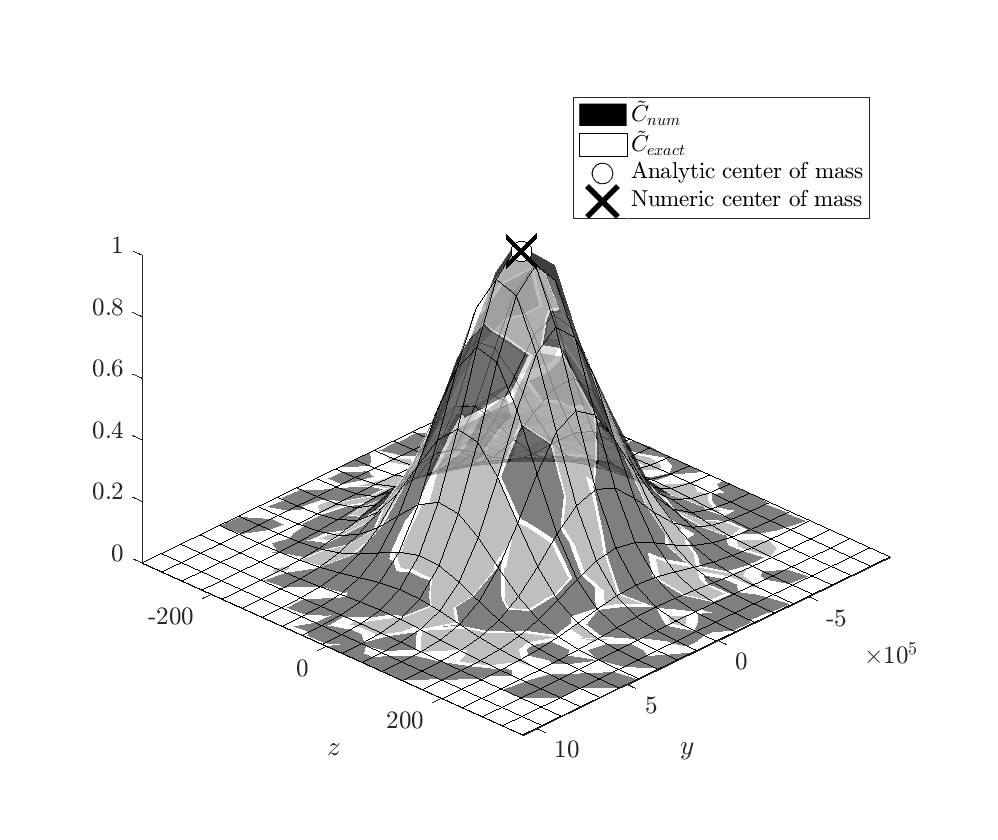
\includegraphics[width = \textwidth]{fig/testcase/testcase_surf.eps}
	\caption{Comparison of the concentrations obtained analytically and numerically. The "centers of mass" of the concentration obtained numerically (black cross) and numerically (white bullet) are also shown on the figure.}
	\label{fig:testcase_surf}
\end{figure}
\begin{figure}[H]
	\centering
	\begin{subfigure}[b]{0.49\textwidth}
		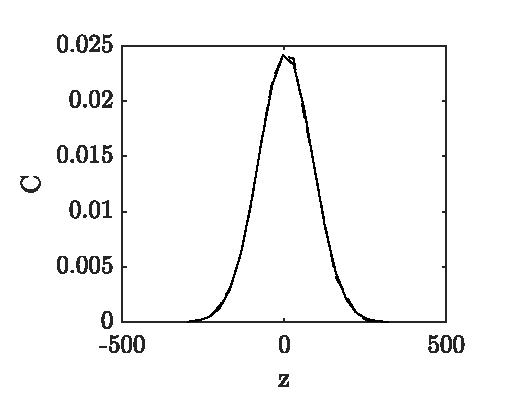
\includegraphics[width=\textwidth]{fig/testcase/testcase_fixedy.eps}
		\caption{$C_{num}(y_1+vT,z)$ and $C_{exact}(y_1+vT,z)$.}
		\label{fig:testcase_fixedy}
	\end{subfigure}
	\begin{subfigure}[b]{0.49\textwidth}
		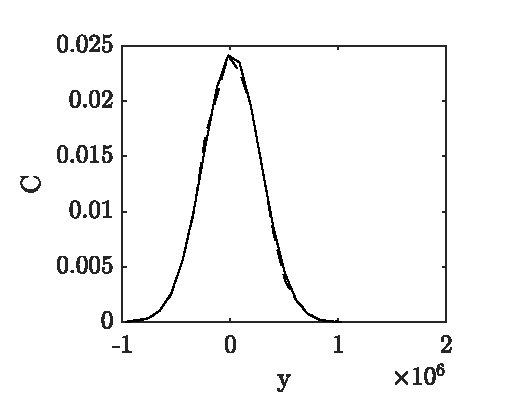
\includegraphics[width=\textwidth]{fig/testcase/testcase_fixedz.eps}
		\caption{$C_{num}(y,z_1+wT)$ and $C_{exact}(y,z_1+wT)$.}
		\label{fig:testcase_fixedz}
	\end{subfigure}
	\caption{Cut of the concentrations at fixed $y = r_{y,exact}$ and at fixed $z = r_{z,exact}$. The dashed line represent $C_{num}$ and the continuous line is for $C_{exact}$.}
\end{figure}

%-------------------------------------------RESULTS CASE 2-----------------------------------------------------------------------%
\subsection{Test case 2}
Figure \ref{fig:testcaseSI_surf} shows a comparison between the numerical result and the analytical solution for the (normalized) concentrations for test case 2. Since we do not have analytical expressions of the center of mass and of the variance for this test case, the "exact" values are approximated numerically thanks to the analytical expression of the concentration. Figures \ref{fig:testcaseSI_fixedy} and \ref{fig:testcaseSI_fixedz} represent respectively a cut of the concentrations at fixed $y = r_{y,exact}$ and along the boundary $z = 0$. The big picture about test case 2 is the presence of a boundary with no-through condition. A first verification is to check if all the particles are still in the domain, which is indeed the case. Although this might seem trivial here, it is sometimes a real challenge to ensure that no particle crosses the boundary, especially for geometrically complex domains. Besides, one can see on figure \ref{fig:testcaseSI_fixedz} that the concentration profile is well approximated along the boundary. Indeed, the maximal local error at the boundary is
\begin{equation}
	\|C_{exact}(y,0)-C_{num}(y,0)\|_{\infty} = 3.53\e{-4}, 
\end{equation}
The maximal local error on the whole domain is 
\begin{equation}
	\|C_{exact}-C_{num}\|_{\infty} = 1.097\e{-3}.
\end{equation}
The centers of mass are located at
\begin{equation}
	\b r_{exact} = (1.26\e{4},5.06\e{3}) \mbox{ [$m$],}\quad \b r_{num} = (1.10\e{4},5.05\e{3}) \mbox{ [$m$]}.
\end{equation}
The relative error is
\begin{equation}
	\b e_r = \left \lvert \frac{\b r_{exact}-\b r_{num}}{\b r_{exact}} \right \rvert =  \left(1.29\e{-1}, 1.825\e{-3}\right).
\end{equation}
The 2-norm of the relative error is
\begin{equation}
	\| \b e_r \|_2 = 1.29\e{-1}.
\end{equation}
This can be seen as a quantification of the error on advection. To quantify the error on diffusion, we compute the variance of the concentration :
\begin{equation}
	\sigma^2_{exact} = 6.39\e{10} \mbox{ [$m^2$],}\quad \sigma^2_{num} = 6.35\e{10} \mbox{ [$m^2$].}
\end{equation}
The relative error is
\begin{equation}
	e_{\sigma^2} = \left \lvert \frac{\sigma^2_{exact}-\sigma^2_{num}}{\sigma^2_{exact}}\right \rvert = 4.85\e{-3}.
\end{equation}
\begin{figure}[H]
	\centering
	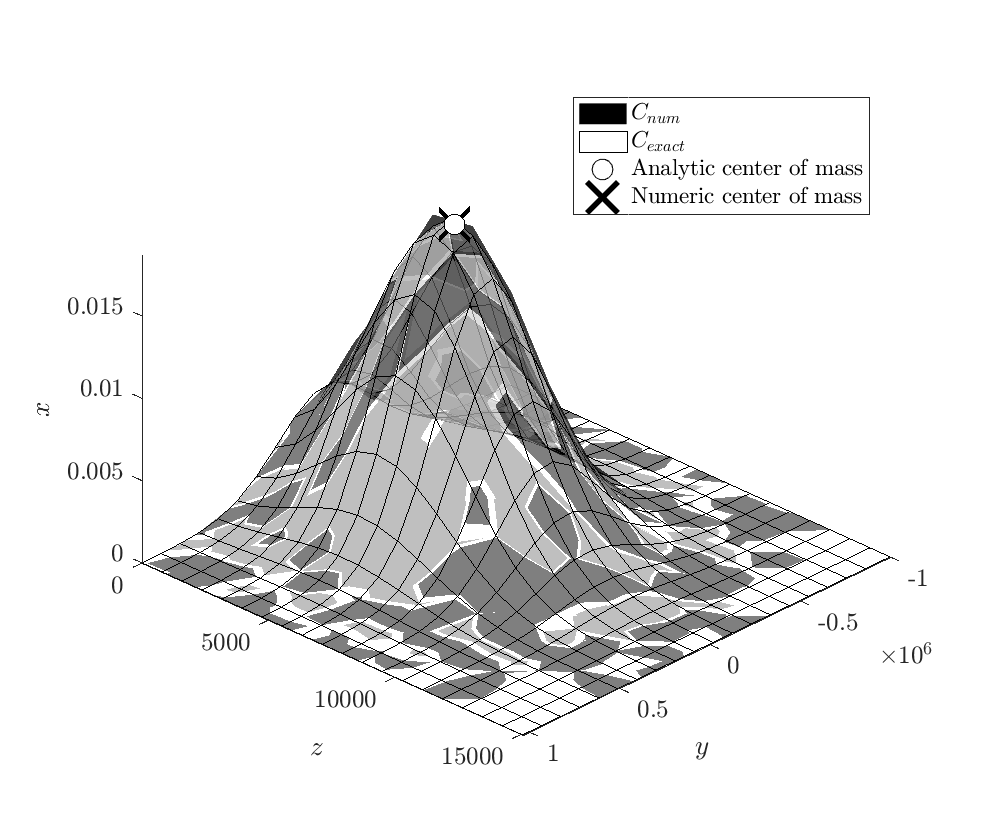
\includegraphics[width = \textwidth]{fig/testcase/testcaseSI_surf.eps}
	\caption{Comparison of the concentrations obtained analytically and numerically. The "centers of mass" of the concentration obtained numerically (black cross) and numerically (white bullet) are also shown on the figure.}
	\label{fig:testcaseSI_surf}
\end{figure}
\begin{figure}[H]
	\centering
	\begin{subfigure}[b]{0.49\textwidth}
		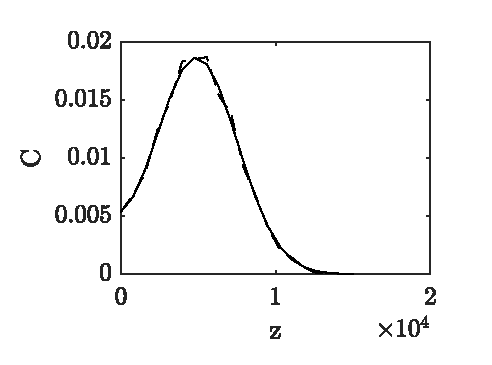
\includegraphics[width=\textwidth]{fig/testcase/testcaseSI_fixedy.eps}
		\caption{$C_{num}(y_1+vT,z)$ and $C_{exact}(y_1+vT,z)$.}
		\label{fig:testcaseSI_fixedy}
	\end{subfigure}
	\begin{subfigure}[b]{0.49\textwidth}
		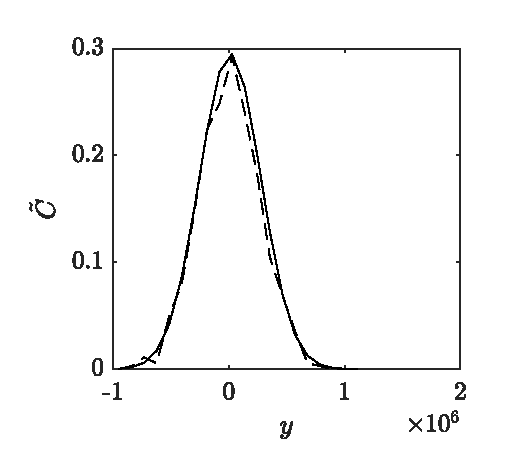
\includegraphics[width=\textwidth]{fig/testcase/testcaseSI_fixedz.eps}
		\caption{$C_{num}(y,z_1+wT)$ and $C_{exact}(y,z_1+wT)$.}
		\label{fig:testcaseSI_fixedz}
	\end{subfigure}
	\caption{Cut of the concentrations at fixed $y = r_{y,exact}$ and at fixed $z = r_{z,exact}$. The dashed line represent $C_{num}$ and the continuous line is for $C_{exact}$.}
\end{figure}
%!TEX root = /home/renaud/Documents/EPL/tfe/latex/tfe.tex
\chapter{From clusters to compartments}
The goal now is to use a clustering algorithm on an advection-diffusion problem, and ultimately use the partitions to build a box-model. The underpinning idea is that communities found on the dynamic of the flow could be relevant compartments for the box-model. The idea makes sense although it is far from being obvious that the communities are indeed the compartments that we seek. In a first instance, we should only check that, at least in some cases, community detection leads to relevant partitions. Hence, we first build a test problem for which we know in advances what compartments to expect. Then we apply the method on the less obvious, though still very naive overturner model of the Atlantic ocean.

\paragraph{Remark} \label{remark:straightboundaries} In the context of interpreting the communities as compartments for a box-model, we should require that the communities have vertical and horizontal boundaries. When dealing with marine problems, the goal of a box-model is to provide a simple and intuitive description of the problem. Complex shaped compartments are neither simple nor intuitive for marine models, hence the requirement.

%!TEX root = /home/renaud/Documents/EPL/tfe/latex/tfe.tex
\section{Methodology}
%-----------------------DESCRIPTION OF THE METHOD---------------------------------%
\subsection{Description of the method}
In order to apply a clustering algorithm on a physical advection-diffusion problem, we have to define how the problem can be considered as a graph. For the next, we consider a two-dimensional problem in the coordinate system $(y,z)$. Let us partition the domain into $\nby \times \nbz$ boxes, and denote $N_{box} = \nby\nbz$ the total number of boxes. Figure~\ref{fig:box_scheme} represents an example of such a domain decomposition of the overturner problem with $\nby = 15$ and $\nbz = 10$. For any time $T$, the corresponding directed graph is build as follows: each node represents a box, and the weight of the edge between nodes $i$ and $j$ is the probability $m_{ij}(T)$ that a particle ends up in box $j$ after a time $T$ if it was initially in box $i$. If $m_{ij}(T) = 0$, one can equivalently consider that there is no edge between nodes $i$ and $j$. Since the problem is stationary, $m_{ij}(T)$ depends only on the elapsed time $T$, not on the initial time. Hence, the initial time can indifferently be considered as being zero. The adjacency matrix $\b M(T)$ of the graph is build from the weights $m_{ij}(T)$: $[\b M(T)]_{ij} = m_{ij}(T)$. For any time $T$, $\b M(T)$ is row-stochastic, i.e. $\b M(T)\b 1 = \b 1$, where $\b 1$ is the $N_{box}$-dimensional unit column vector. The latter has a straightforward physical interpretation: every particle remains in the domain.

\begin{figure}[!htp]
	\centering
	% This file was created by matlab2tikz.
%
%The latest updates can be retrieved from
%  http://www.mathworks.com/matlabcentral/fileexchange/22022-matlab2tikz-matlab2tikz
%where you can also make suggestions and rate matlab2tikz.
%
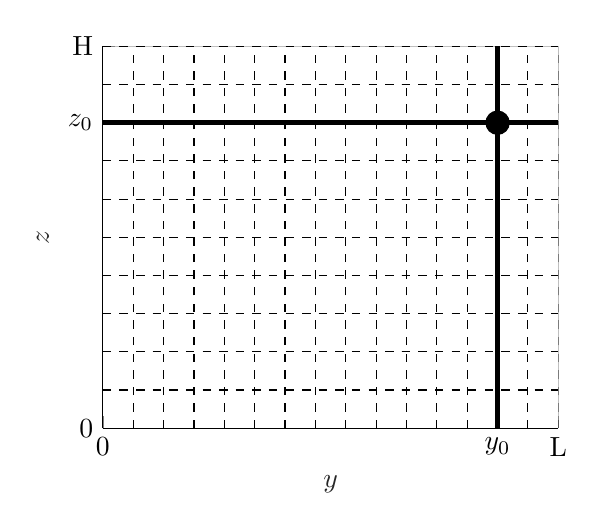
\begin{tikzpicture}

\begin{axis}[%
width=0.477\textwidth,
height=0.4\textwidth,
at={(0\textwidth,0\textwidth)},
scale only axis,
xmin=0,
xmax=15,
xtick={0,13,15},
xticklabels={{0},{$y_0$},{L}},
xlabel style={font=\color{white!15!black}},
xlabel={$y$},
ymin=0,
ymax=5,
ytick={0,4,5},
yticklabels={{0},{$z_0$},{H}},
ylabel style={font=\color{white!15!black}},
ylabel={$z$},
axis background/.style={fill=white},
axis x line*=bottom,
axis y line*=left,
xmajorgrids,
ymajorgrids
]
\addplot [color=black, dashed, forget plot]
  table[row sep=crcr]{%
0	0\\
0	0.0505050505050505\\
0	0.101010101010101\\
0	0.151515151515152\\
0	0.202020202020202\\
0	0.252525252525253\\
0	0.303030303030303\\
0	0.353535353535354\\
0	0.404040404040404\\
0	0.454545454545455\\
0	0.505050505050505\\
0	0.555555555555556\\
0	0.606060606060606\\
0	0.656565656565657\\
0	0.707070707070707\\
0	0.757575757575758\\
0	0.808080808080808\\
0	0.858585858585859\\
0	0.909090909090909\\
0	0.95959595959596\\
0	1.01010101010101\\
0	1.06060606060606\\
0	1.11111111111111\\
0	1.16161616161616\\
0	1.21212121212121\\
0	1.26262626262626\\
0	1.31313131313131\\
0	1.36363636363636\\
0	1.41414141414141\\
0	1.46464646464646\\
0	1.51515151515152\\
0	1.56565656565657\\
0	1.61616161616162\\
0	1.66666666666667\\
0	1.71717171717172\\
0	1.76767676767677\\
0	1.81818181818182\\
0	1.86868686868687\\
0	1.91919191919192\\
0	1.96969696969697\\
0	2.02020202020202\\
0	2.07070707070707\\
0	2.12121212121212\\
0	2.17171717171717\\
0	2.22222222222222\\
0	2.27272727272727\\
0	2.32323232323232\\
0	2.37373737373737\\
0	2.42424242424242\\
0	2.47474747474747\\
0	2.52525252525253\\
0	2.57575757575758\\
0	2.62626262626263\\
0	2.67676767676768\\
0	2.72727272727273\\
0	2.77777777777778\\
0	2.82828282828283\\
0	2.87878787878788\\
0	2.92929292929293\\
0	2.97979797979798\\
0	3.03030303030303\\
0	3.08080808080808\\
0	3.13131313131313\\
0	3.18181818181818\\
0	3.23232323232323\\
0	3.28282828282828\\
0	3.33333333333333\\
0	3.38383838383838\\
0	3.43434343434343\\
0	3.48484848484848\\
0	3.53535353535354\\
0	3.58585858585859\\
0	3.63636363636364\\
0	3.68686868686869\\
0	3.73737373737374\\
0	3.78787878787879\\
0	3.83838383838384\\
0	3.88888888888889\\
0	3.93939393939394\\
0	3.98989898989899\\
0	4.04040404040404\\
0	4.09090909090909\\
0	4.14141414141414\\
0	4.19191919191919\\
0	4.24242424242424\\
0	4.29292929292929\\
0	4.34343434343434\\
0	4.39393939393939\\
0	4.44444444444444\\
0	4.49494949494949\\
0	4.54545454545455\\
0	4.5959595959596\\
0	4.64646464646465\\
0	4.6969696969697\\
0	4.74747474747475\\
0	4.7979797979798\\
0	4.84848484848485\\
0	4.8989898989899\\
0	4.94949494949495\\
0	5\\
};
\addplot [color=black, dashed, forget plot]
  table[row sep=crcr]{%
1	0\\
1	0.0505050505050505\\
1	0.101010101010101\\
1	0.151515151515152\\
1	0.202020202020202\\
1	0.252525252525253\\
1	0.303030303030303\\
1	0.353535353535354\\
1	0.404040404040404\\
1	0.454545454545455\\
1	0.505050505050505\\
1	0.555555555555556\\
1	0.606060606060606\\
1	0.656565656565657\\
1	0.707070707070707\\
1	0.757575757575758\\
1	0.808080808080808\\
1	0.858585858585859\\
1	0.909090909090909\\
1	0.95959595959596\\
1	1.01010101010101\\
1	1.06060606060606\\
1	1.11111111111111\\
1	1.16161616161616\\
1	1.21212121212121\\
1	1.26262626262626\\
1	1.31313131313131\\
1	1.36363636363636\\
1	1.41414141414141\\
1	1.46464646464646\\
1	1.51515151515152\\
1	1.56565656565657\\
1	1.61616161616162\\
1	1.66666666666667\\
1	1.71717171717172\\
1	1.76767676767677\\
1	1.81818181818182\\
1	1.86868686868687\\
1	1.91919191919192\\
1	1.96969696969697\\
1	2.02020202020202\\
1	2.07070707070707\\
1	2.12121212121212\\
1	2.17171717171717\\
1	2.22222222222222\\
1	2.27272727272727\\
1	2.32323232323232\\
1	2.37373737373737\\
1	2.42424242424242\\
1	2.47474747474747\\
1	2.52525252525253\\
1	2.57575757575758\\
1	2.62626262626263\\
1	2.67676767676768\\
1	2.72727272727273\\
1	2.77777777777778\\
1	2.82828282828283\\
1	2.87878787878788\\
1	2.92929292929293\\
1	2.97979797979798\\
1	3.03030303030303\\
1	3.08080808080808\\
1	3.13131313131313\\
1	3.18181818181818\\
1	3.23232323232323\\
1	3.28282828282828\\
1	3.33333333333333\\
1	3.38383838383838\\
1	3.43434343434343\\
1	3.48484848484848\\
1	3.53535353535354\\
1	3.58585858585859\\
1	3.63636363636364\\
1	3.68686868686869\\
1	3.73737373737374\\
1	3.78787878787879\\
1	3.83838383838384\\
1	3.88888888888889\\
1	3.93939393939394\\
1	3.98989898989899\\
1	4.04040404040404\\
1	4.09090909090909\\
1	4.14141414141414\\
1	4.19191919191919\\
1	4.24242424242424\\
1	4.29292929292929\\
1	4.34343434343434\\
1	4.39393939393939\\
1	4.44444444444444\\
1	4.49494949494949\\
1	4.54545454545455\\
1	4.5959595959596\\
1	4.64646464646465\\
1	4.6969696969697\\
1	4.74747474747475\\
1	4.7979797979798\\
1	4.84848484848485\\
1	4.8989898989899\\
1	4.94949494949495\\
1	5\\
};
\addplot [color=black, dashed, forget plot]
  table[row sep=crcr]{%
2	0\\
2	0.0505050505050505\\
2	0.101010101010101\\
2	0.151515151515152\\
2	0.202020202020202\\
2	0.252525252525253\\
2	0.303030303030303\\
2	0.353535353535354\\
2	0.404040404040404\\
2	0.454545454545455\\
2	0.505050505050505\\
2	0.555555555555556\\
2	0.606060606060606\\
2	0.656565656565657\\
2	0.707070707070707\\
2	0.757575757575758\\
2	0.808080808080808\\
2	0.858585858585859\\
2	0.909090909090909\\
2	0.95959595959596\\
2	1.01010101010101\\
2	1.06060606060606\\
2	1.11111111111111\\
2	1.16161616161616\\
2	1.21212121212121\\
2	1.26262626262626\\
2	1.31313131313131\\
2	1.36363636363636\\
2	1.41414141414141\\
2	1.46464646464646\\
2	1.51515151515152\\
2	1.56565656565657\\
2	1.61616161616162\\
2	1.66666666666667\\
2	1.71717171717172\\
2	1.76767676767677\\
2	1.81818181818182\\
2	1.86868686868687\\
2	1.91919191919192\\
2	1.96969696969697\\
2	2.02020202020202\\
2	2.07070707070707\\
2	2.12121212121212\\
2	2.17171717171717\\
2	2.22222222222222\\
2	2.27272727272727\\
2	2.32323232323232\\
2	2.37373737373737\\
2	2.42424242424242\\
2	2.47474747474747\\
2	2.52525252525253\\
2	2.57575757575758\\
2	2.62626262626263\\
2	2.67676767676768\\
2	2.72727272727273\\
2	2.77777777777778\\
2	2.82828282828283\\
2	2.87878787878788\\
2	2.92929292929293\\
2	2.97979797979798\\
2	3.03030303030303\\
2	3.08080808080808\\
2	3.13131313131313\\
2	3.18181818181818\\
2	3.23232323232323\\
2	3.28282828282828\\
2	3.33333333333333\\
2	3.38383838383838\\
2	3.43434343434343\\
2	3.48484848484848\\
2	3.53535353535354\\
2	3.58585858585859\\
2	3.63636363636364\\
2	3.68686868686869\\
2	3.73737373737374\\
2	3.78787878787879\\
2	3.83838383838384\\
2	3.88888888888889\\
2	3.93939393939394\\
2	3.98989898989899\\
2	4.04040404040404\\
2	4.09090909090909\\
2	4.14141414141414\\
2	4.19191919191919\\
2	4.24242424242424\\
2	4.29292929292929\\
2	4.34343434343434\\
2	4.39393939393939\\
2	4.44444444444444\\
2	4.49494949494949\\
2	4.54545454545455\\
2	4.5959595959596\\
2	4.64646464646465\\
2	4.6969696969697\\
2	4.74747474747475\\
2	4.7979797979798\\
2	4.84848484848485\\
2	4.8989898989899\\
2	4.94949494949495\\
2	5\\
};
\addplot [color=black, dashed, forget plot]
  table[row sep=crcr]{%
3	0\\
3	0.0505050505050505\\
3	0.101010101010101\\
3	0.151515151515152\\
3	0.202020202020202\\
3	0.252525252525253\\
3	0.303030303030303\\
3	0.353535353535354\\
3	0.404040404040404\\
3	0.454545454545455\\
3	0.505050505050505\\
3	0.555555555555556\\
3	0.606060606060606\\
3	0.656565656565657\\
3	0.707070707070707\\
3	0.757575757575758\\
3	0.808080808080808\\
3	0.858585858585859\\
3	0.909090909090909\\
3	0.95959595959596\\
3	1.01010101010101\\
3	1.06060606060606\\
3	1.11111111111111\\
3	1.16161616161616\\
3	1.21212121212121\\
3	1.26262626262626\\
3	1.31313131313131\\
3	1.36363636363636\\
3	1.41414141414141\\
3	1.46464646464646\\
3	1.51515151515152\\
3	1.56565656565657\\
3	1.61616161616162\\
3	1.66666666666667\\
3	1.71717171717172\\
3	1.76767676767677\\
3	1.81818181818182\\
3	1.86868686868687\\
3	1.91919191919192\\
3	1.96969696969697\\
3	2.02020202020202\\
3	2.07070707070707\\
3	2.12121212121212\\
3	2.17171717171717\\
3	2.22222222222222\\
3	2.27272727272727\\
3	2.32323232323232\\
3	2.37373737373737\\
3	2.42424242424242\\
3	2.47474747474747\\
3	2.52525252525253\\
3	2.57575757575758\\
3	2.62626262626263\\
3	2.67676767676768\\
3	2.72727272727273\\
3	2.77777777777778\\
3	2.82828282828283\\
3	2.87878787878788\\
3	2.92929292929293\\
3	2.97979797979798\\
3	3.03030303030303\\
3	3.08080808080808\\
3	3.13131313131313\\
3	3.18181818181818\\
3	3.23232323232323\\
3	3.28282828282828\\
3	3.33333333333333\\
3	3.38383838383838\\
3	3.43434343434343\\
3	3.48484848484848\\
3	3.53535353535354\\
3	3.58585858585859\\
3	3.63636363636364\\
3	3.68686868686869\\
3	3.73737373737374\\
3	3.78787878787879\\
3	3.83838383838384\\
3	3.88888888888889\\
3	3.93939393939394\\
3	3.98989898989899\\
3	4.04040404040404\\
3	4.09090909090909\\
3	4.14141414141414\\
3	4.19191919191919\\
3	4.24242424242424\\
3	4.29292929292929\\
3	4.34343434343434\\
3	4.39393939393939\\
3	4.44444444444444\\
3	4.49494949494949\\
3	4.54545454545455\\
3	4.5959595959596\\
3	4.64646464646465\\
3	4.6969696969697\\
3	4.74747474747475\\
3	4.7979797979798\\
3	4.84848484848485\\
3	4.8989898989899\\
3	4.94949494949495\\
3	5\\
};
\addplot [color=black, dashed, forget plot]
  table[row sep=crcr]{%
4	0\\
4	0.0505050505050505\\
4	0.101010101010101\\
4	0.151515151515152\\
4	0.202020202020202\\
4	0.252525252525253\\
4	0.303030303030303\\
4	0.353535353535354\\
4	0.404040404040404\\
4	0.454545454545455\\
4	0.505050505050505\\
4	0.555555555555556\\
4	0.606060606060606\\
4	0.656565656565657\\
4	0.707070707070707\\
4	0.757575757575758\\
4	0.808080808080808\\
4	0.858585858585859\\
4	0.909090909090909\\
4	0.95959595959596\\
4	1.01010101010101\\
4	1.06060606060606\\
4	1.11111111111111\\
4	1.16161616161616\\
4	1.21212121212121\\
4	1.26262626262626\\
4	1.31313131313131\\
4	1.36363636363636\\
4	1.41414141414141\\
4	1.46464646464646\\
4	1.51515151515152\\
4	1.56565656565657\\
4	1.61616161616162\\
4	1.66666666666667\\
4	1.71717171717172\\
4	1.76767676767677\\
4	1.81818181818182\\
4	1.86868686868687\\
4	1.91919191919192\\
4	1.96969696969697\\
4	2.02020202020202\\
4	2.07070707070707\\
4	2.12121212121212\\
4	2.17171717171717\\
4	2.22222222222222\\
4	2.27272727272727\\
4	2.32323232323232\\
4	2.37373737373737\\
4	2.42424242424242\\
4	2.47474747474747\\
4	2.52525252525253\\
4	2.57575757575758\\
4	2.62626262626263\\
4	2.67676767676768\\
4	2.72727272727273\\
4	2.77777777777778\\
4	2.82828282828283\\
4	2.87878787878788\\
4	2.92929292929293\\
4	2.97979797979798\\
4	3.03030303030303\\
4	3.08080808080808\\
4	3.13131313131313\\
4	3.18181818181818\\
4	3.23232323232323\\
4	3.28282828282828\\
4	3.33333333333333\\
4	3.38383838383838\\
4	3.43434343434343\\
4	3.48484848484848\\
4	3.53535353535354\\
4	3.58585858585859\\
4	3.63636363636364\\
4	3.68686868686869\\
4	3.73737373737374\\
4	3.78787878787879\\
4	3.83838383838384\\
4	3.88888888888889\\
4	3.93939393939394\\
4	3.98989898989899\\
4	4.04040404040404\\
4	4.09090909090909\\
4	4.14141414141414\\
4	4.19191919191919\\
4	4.24242424242424\\
4	4.29292929292929\\
4	4.34343434343434\\
4	4.39393939393939\\
4	4.44444444444444\\
4	4.49494949494949\\
4	4.54545454545455\\
4	4.5959595959596\\
4	4.64646464646465\\
4	4.6969696969697\\
4	4.74747474747475\\
4	4.7979797979798\\
4	4.84848484848485\\
4	4.8989898989899\\
4	4.94949494949495\\
4	5\\
};
\addplot [color=black, dashed, forget plot]
  table[row sep=crcr]{%
5	0\\
5	0.0505050505050505\\
5	0.101010101010101\\
5	0.151515151515152\\
5	0.202020202020202\\
5	0.252525252525253\\
5	0.303030303030303\\
5	0.353535353535354\\
5	0.404040404040404\\
5	0.454545454545455\\
5	0.505050505050505\\
5	0.555555555555556\\
5	0.606060606060606\\
5	0.656565656565657\\
5	0.707070707070707\\
5	0.757575757575758\\
5	0.808080808080808\\
5	0.858585858585859\\
5	0.909090909090909\\
5	0.95959595959596\\
5	1.01010101010101\\
5	1.06060606060606\\
5	1.11111111111111\\
5	1.16161616161616\\
5	1.21212121212121\\
5	1.26262626262626\\
5	1.31313131313131\\
5	1.36363636363636\\
5	1.41414141414141\\
5	1.46464646464646\\
5	1.51515151515152\\
5	1.56565656565657\\
5	1.61616161616162\\
5	1.66666666666667\\
5	1.71717171717172\\
5	1.76767676767677\\
5	1.81818181818182\\
5	1.86868686868687\\
5	1.91919191919192\\
5	1.96969696969697\\
5	2.02020202020202\\
5	2.07070707070707\\
5	2.12121212121212\\
5	2.17171717171717\\
5	2.22222222222222\\
5	2.27272727272727\\
5	2.32323232323232\\
5	2.37373737373737\\
5	2.42424242424242\\
5	2.47474747474747\\
5	2.52525252525253\\
5	2.57575757575758\\
5	2.62626262626263\\
5	2.67676767676768\\
5	2.72727272727273\\
5	2.77777777777778\\
5	2.82828282828283\\
5	2.87878787878788\\
5	2.92929292929293\\
5	2.97979797979798\\
5	3.03030303030303\\
5	3.08080808080808\\
5	3.13131313131313\\
5	3.18181818181818\\
5	3.23232323232323\\
5	3.28282828282828\\
5	3.33333333333333\\
5	3.38383838383838\\
5	3.43434343434343\\
5	3.48484848484848\\
5	3.53535353535354\\
5	3.58585858585859\\
5	3.63636363636364\\
5	3.68686868686869\\
5	3.73737373737374\\
5	3.78787878787879\\
5	3.83838383838384\\
5	3.88888888888889\\
5	3.93939393939394\\
5	3.98989898989899\\
5	4.04040404040404\\
5	4.09090909090909\\
5	4.14141414141414\\
5	4.19191919191919\\
5	4.24242424242424\\
5	4.29292929292929\\
5	4.34343434343434\\
5	4.39393939393939\\
5	4.44444444444444\\
5	4.49494949494949\\
5	4.54545454545455\\
5	4.5959595959596\\
5	4.64646464646465\\
5	4.6969696969697\\
5	4.74747474747475\\
5	4.7979797979798\\
5	4.84848484848485\\
5	4.8989898989899\\
5	4.94949494949495\\
5	5\\
};
\addplot [color=black, dashed, forget plot]
  table[row sep=crcr]{%
6	0\\
6	0.0505050505050505\\
6	0.101010101010101\\
6	0.151515151515152\\
6	0.202020202020202\\
6	0.252525252525253\\
6	0.303030303030303\\
6	0.353535353535354\\
6	0.404040404040404\\
6	0.454545454545455\\
6	0.505050505050505\\
6	0.555555555555556\\
6	0.606060606060606\\
6	0.656565656565657\\
6	0.707070707070707\\
6	0.757575757575758\\
6	0.808080808080808\\
6	0.858585858585859\\
6	0.909090909090909\\
6	0.95959595959596\\
6	1.01010101010101\\
6	1.06060606060606\\
6	1.11111111111111\\
6	1.16161616161616\\
6	1.21212121212121\\
6	1.26262626262626\\
6	1.31313131313131\\
6	1.36363636363636\\
6	1.41414141414141\\
6	1.46464646464646\\
6	1.51515151515152\\
6	1.56565656565657\\
6	1.61616161616162\\
6	1.66666666666667\\
6	1.71717171717172\\
6	1.76767676767677\\
6	1.81818181818182\\
6	1.86868686868687\\
6	1.91919191919192\\
6	1.96969696969697\\
6	2.02020202020202\\
6	2.07070707070707\\
6	2.12121212121212\\
6	2.17171717171717\\
6	2.22222222222222\\
6	2.27272727272727\\
6	2.32323232323232\\
6	2.37373737373737\\
6	2.42424242424242\\
6	2.47474747474747\\
6	2.52525252525253\\
6	2.57575757575758\\
6	2.62626262626263\\
6	2.67676767676768\\
6	2.72727272727273\\
6	2.77777777777778\\
6	2.82828282828283\\
6	2.87878787878788\\
6	2.92929292929293\\
6	2.97979797979798\\
6	3.03030303030303\\
6	3.08080808080808\\
6	3.13131313131313\\
6	3.18181818181818\\
6	3.23232323232323\\
6	3.28282828282828\\
6	3.33333333333333\\
6	3.38383838383838\\
6	3.43434343434343\\
6	3.48484848484848\\
6	3.53535353535354\\
6	3.58585858585859\\
6	3.63636363636364\\
6	3.68686868686869\\
6	3.73737373737374\\
6	3.78787878787879\\
6	3.83838383838384\\
6	3.88888888888889\\
6	3.93939393939394\\
6	3.98989898989899\\
6	4.04040404040404\\
6	4.09090909090909\\
6	4.14141414141414\\
6	4.19191919191919\\
6	4.24242424242424\\
6	4.29292929292929\\
6	4.34343434343434\\
6	4.39393939393939\\
6	4.44444444444444\\
6	4.49494949494949\\
6	4.54545454545455\\
6	4.5959595959596\\
6	4.64646464646465\\
6	4.6969696969697\\
6	4.74747474747475\\
6	4.7979797979798\\
6	4.84848484848485\\
6	4.8989898989899\\
6	4.94949494949495\\
6	5\\
};
\addplot [color=black, dashed, forget plot]
  table[row sep=crcr]{%
7	0\\
7	0.0505050505050505\\
7	0.101010101010101\\
7	0.151515151515152\\
7	0.202020202020202\\
7	0.252525252525253\\
7	0.303030303030303\\
7	0.353535353535354\\
7	0.404040404040404\\
7	0.454545454545455\\
7	0.505050505050505\\
7	0.555555555555556\\
7	0.606060606060606\\
7	0.656565656565657\\
7	0.707070707070707\\
7	0.757575757575758\\
7	0.808080808080808\\
7	0.858585858585859\\
7	0.909090909090909\\
7	0.95959595959596\\
7	1.01010101010101\\
7	1.06060606060606\\
7	1.11111111111111\\
7	1.16161616161616\\
7	1.21212121212121\\
7	1.26262626262626\\
7	1.31313131313131\\
7	1.36363636363636\\
7	1.41414141414141\\
7	1.46464646464646\\
7	1.51515151515152\\
7	1.56565656565657\\
7	1.61616161616162\\
7	1.66666666666667\\
7	1.71717171717172\\
7	1.76767676767677\\
7	1.81818181818182\\
7	1.86868686868687\\
7	1.91919191919192\\
7	1.96969696969697\\
7	2.02020202020202\\
7	2.07070707070707\\
7	2.12121212121212\\
7	2.17171717171717\\
7	2.22222222222222\\
7	2.27272727272727\\
7	2.32323232323232\\
7	2.37373737373737\\
7	2.42424242424242\\
7	2.47474747474747\\
7	2.52525252525253\\
7	2.57575757575758\\
7	2.62626262626263\\
7	2.67676767676768\\
7	2.72727272727273\\
7	2.77777777777778\\
7	2.82828282828283\\
7	2.87878787878788\\
7	2.92929292929293\\
7	2.97979797979798\\
7	3.03030303030303\\
7	3.08080808080808\\
7	3.13131313131313\\
7	3.18181818181818\\
7	3.23232323232323\\
7	3.28282828282828\\
7	3.33333333333333\\
7	3.38383838383838\\
7	3.43434343434343\\
7	3.48484848484848\\
7	3.53535353535354\\
7	3.58585858585859\\
7	3.63636363636364\\
7	3.68686868686869\\
7	3.73737373737374\\
7	3.78787878787879\\
7	3.83838383838384\\
7	3.88888888888889\\
7	3.93939393939394\\
7	3.98989898989899\\
7	4.04040404040404\\
7	4.09090909090909\\
7	4.14141414141414\\
7	4.19191919191919\\
7	4.24242424242424\\
7	4.29292929292929\\
7	4.34343434343434\\
7	4.39393939393939\\
7	4.44444444444444\\
7	4.49494949494949\\
7	4.54545454545455\\
7	4.5959595959596\\
7	4.64646464646465\\
7	4.6969696969697\\
7	4.74747474747475\\
7	4.7979797979798\\
7	4.84848484848485\\
7	4.8989898989899\\
7	4.94949494949495\\
7	5\\
};
\addplot [color=black, dashed, forget plot]
  table[row sep=crcr]{%
8	0\\
8	0.0505050505050505\\
8	0.101010101010101\\
8	0.151515151515152\\
8	0.202020202020202\\
8	0.252525252525253\\
8	0.303030303030303\\
8	0.353535353535354\\
8	0.404040404040404\\
8	0.454545454545455\\
8	0.505050505050505\\
8	0.555555555555556\\
8	0.606060606060606\\
8	0.656565656565657\\
8	0.707070707070707\\
8	0.757575757575758\\
8	0.808080808080808\\
8	0.858585858585859\\
8	0.909090909090909\\
8	0.95959595959596\\
8	1.01010101010101\\
8	1.06060606060606\\
8	1.11111111111111\\
8	1.16161616161616\\
8	1.21212121212121\\
8	1.26262626262626\\
8	1.31313131313131\\
8	1.36363636363636\\
8	1.41414141414141\\
8	1.46464646464646\\
8	1.51515151515152\\
8	1.56565656565657\\
8	1.61616161616162\\
8	1.66666666666667\\
8	1.71717171717172\\
8	1.76767676767677\\
8	1.81818181818182\\
8	1.86868686868687\\
8	1.91919191919192\\
8	1.96969696969697\\
8	2.02020202020202\\
8	2.07070707070707\\
8	2.12121212121212\\
8	2.17171717171717\\
8	2.22222222222222\\
8	2.27272727272727\\
8	2.32323232323232\\
8	2.37373737373737\\
8	2.42424242424242\\
8	2.47474747474747\\
8	2.52525252525253\\
8	2.57575757575758\\
8	2.62626262626263\\
8	2.67676767676768\\
8	2.72727272727273\\
8	2.77777777777778\\
8	2.82828282828283\\
8	2.87878787878788\\
8	2.92929292929293\\
8	2.97979797979798\\
8	3.03030303030303\\
8	3.08080808080808\\
8	3.13131313131313\\
8	3.18181818181818\\
8	3.23232323232323\\
8	3.28282828282828\\
8	3.33333333333333\\
8	3.38383838383838\\
8	3.43434343434343\\
8	3.48484848484848\\
8	3.53535353535354\\
8	3.58585858585859\\
8	3.63636363636364\\
8	3.68686868686869\\
8	3.73737373737374\\
8	3.78787878787879\\
8	3.83838383838384\\
8	3.88888888888889\\
8	3.93939393939394\\
8	3.98989898989899\\
8	4.04040404040404\\
8	4.09090909090909\\
8	4.14141414141414\\
8	4.19191919191919\\
8	4.24242424242424\\
8	4.29292929292929\\
8	4.34343434343434\\
8	4.39393939393939\\
8	4.44444444444444\\
8	4.49494949494949\\
8	4.54545454545455\\
8	4.5959595959596\\
8	4.64646464646465\\
8	4.6969696969697\\
8	4.74747474747475\\
8	4.7979797979798\\
8	4.84848484848485\\
8	4.8989898989899\\
8	4.94949494949495\\
8	5\\
};
\addplot [color=black, dashed, forget plot]
  table[row sep=crcr]{%
9	0\\
9	0.0505050505050505\\
9	0.101010101010101\\
9	0.151515151515152\\
9	0.202020202020202\\
9	0.252525252525253\\
9	0.303030303030303\\
9	0.353535353535354\\
9	0.404040404040404\\
9	0.454545454545455\\
9	0.505050505050505\\
9	0.555555555555556\\
9	0.606060606060606\\
9	0.656565656565657\\
9	0.707070707070707\\
9	0.757575757575758\\
9	0.808080808080808\\
9	0.858585858585859\\
9	0.909090909090909\\
9	0.95959595959596\\
9	1.01010101010101\\
9	1.06060606060606\\
9	1.11111111111111\\
9	1.16161616161616\\
9	1.21212121212121\\
9	1.26262626262626\\
9	1.31313131313131\\
9	1.36363636363636\\
9	1.41414141414141\\
9	1.46464646464646\\
9	1.51515151515152\\
9	1.56565656565657\\
9	1.61616161616162\\
9	1.66666666666667\\
9	1.71717171717172\\
9	1.76767676767677\\
9	1.81818181818182\\
9	1.86868686868687\\
9	1.91919191919192\\
9	1.96969696969697\\
9	2.02020202020202\\
9	2.07070707070707\\
9	2.12121212121212\\
9	2.17171717171717\\
9	2.22222222222222\\
9	2.27272727272727\\
9	2.32323232323232\\
9	2.37373737373737\\
9	2.42424242424242\\
9	2.47474747474747\\
9	2.52525252525253\\
9	2.57575757575758\\
9	2.62626262626263\\
9	2.67676767676768\\
9	2.72727272727273\\
9	2.77777777777778\\
9	2.82828282828283\\
9	2.87878787878788\\
9	2.92929292929293\\
9	2.97979797979798\\
9	3.03030303030303\\
9	3.08080808080808\\
9	3.13131313131313\\
9	3.18181818181818\\
9	3.23232323232323\\
9	3.28282828282828\\
9	3.33333333333333\\
9	3.38383838383838\\
9	3.43434343434343\\
9	3.48484848484848\\
9	3.53535353535354\\
9	3.58585858585859\\
9	3.63636363636364\\
9	3.68686868686869\\
9	3.73737373737374\\
9	3.78787878787879\\
9	3.83838383838384\\
9	3.88888888888889\\
9	3.93939393939394\\
9	3.98989898989899\\
9	4.04040404040404\\
9	4.09090909090909\\
9	4.14141414141414\\
9	4.19191919191919\\
9	4.24242424242424\\
9	4.29292929292929\\
9	4.34343434343434\\
9	4.39393939393939\\
9	4.44444444444444\\
9	4.49494949494949\\
9	4.54545454545455\\
9	4.5959595959596\\
9	4.64646464646465\\
9	4.6969696969697\\
9	4.74747474747475\\
9	4.7979797979798\\
9	4.84848484848485\\
9	4.8989898989899\\
9	4.94949494949495\\
9	5\\
};
\addplot [color=black, dashed, forget plot]
  table[row sep=crcr]{%
10	0\\
10	0.0505050505050505\\
10	0.101010101010101\\
10	0.151515151515152\\
10	0.202020202020202\\
10	0.252525252525253\\
10	0.303030303030303\\
10	0.353535353535354\\
10	0.404040404040404\\
10	0.454545454545455\\
10	0.505050505050505\\
10	0.555555555555556\\
10	0.606060606060606\\
10	0.656565656565657\\
10	0.707070707070707\\
10	0.757575757575758\\
10	0.808080808080808\\
10	0.858585858585859\\
10	0.909090909090909\\
10	0.95959595959596\\
10	1.01010101010101\\
10	1.06060606060606\\
10	1.11111111111111\\
10	1.16161616161616\\
10	1.21212121212121\\
10	1.26262626262626\\
10	1.31313131313131\\
10	1.36363636363636\\
10	1.41414141414141\\
10	1.46464646464646\\
10	1.51515151515152\\
10	1.56565656565657\\
10	1.61616161616162\\
10	1.66666666666667\\
10	1.71717171717172\\
10	1.76767676767677\\
10	1.81818181818182\\
10	1.86868686868687\\
10	1.91919191919192\\
10	1.96969696969697\\
10	2.02020202020202\\
10	2.07070707070707\\
10	2.12121212121212\\
10	2.17171717171717\\
10	2.22222222222222\\
10	2.27272727272727\\
10	2.32323232323232\\
10	2.37373737373737\\
10	2.42424242424242\\
10	2.47474747474747\\
10	2.52525252525253\\
10	2.57575757575758\\
10	2.62626262626263\\
10	2.67676767676768\\
10	2.72727272727273\\
10	2.77777777777778\\
10	2.82828282828283\\
10	2.87878787878788\\
10	2.92929292929293\\
10	2.97979797979798\\
10	3.03030303030303\\
10	3.08080808080808\\
10	3.13131313131313\\
10	3.18181818181818\\
10	3.23232323232323\\
10	3.28282828282828\\
10	3.33333333333333\\
10	3.38383838383838\\
10	3.43434343434343\\
10	3.48484848484848\\
10	3.53535353535354\\
10	3.58585858585859\\
10	3.63636363636364\\
10	3.68686868686869\\
10	3.73737373737374\\
10	3.78787878787879\\
10	3.83838383838384\\
10	3.88888888888889\\
10	3.93939393939394\\
10	3.98989898989899\\
10	4.04040404040404\\
10	4.09090909090909\\
10	4.14141414141414\\
10	4.19191919191919\\
10	4.24242424242424\\
10	4.29292929292929\\
10	4.34343434343434\\
10	4.39393939393939\\
10	4.44444444444444\\
10	4.49494949494949\\
10	4.54545454545455\\
10	4.5959595959596\\
10	4.64646464646465\\
10	4.6969696969697\\
10	4.74747474747475\\
10	4.7979797979798\\
10	4.84848484848485\\
10	4.8989898989899\\
10	4.94949494949495\\
10	5\\
};
\addplot [color=black, dashed, forget plot]
  table[row sep=crcr]{%
11	0\\
11	0.0505050505050505\\
11	0.101010101010101\\
11	0.151515151515152\\
11	0.202020202020202\\
11	0.252525252525253\\
11	0.303030303030303\\
11	0.353535353535354\\
11	0.404040404040404\\
11	0.454545454545455\\
11	0.505050505050505\\
11	0.555555555555556\\
11	0.606060606060606\\
11	0.656565656565657\\
11	0.707070707070707\\
11	0.757575757575758\\
11	0.808080808080808\\
11	0.858585858585859\\
11	0.909090909090909\\
11	0.95959595959596\\
11	1.01010101010101\\
11	1.06060606060606\\
11	1.11111111111111\\
11	1.16161616161616\\
11	1.21212121212121\\
11	1.26262626262626\\
11	1.31313131313131\\
11	1.36363636363636\\
11	1.41414141414141\\
11	1.46464646464646\\
11	1.51515151515152\\
11	1.56565656565657\\
11	1.61616161616162\\
11	1.66666666666667\\
11	1.71717171717172\\
11	1.76767676767677\\
11	1.81818181818182\\
11	1.86868686868687\\
11	1.91919191919192\\
11	1.96969696969697\\
11	2.02020202020202\\
11	2.07070707070707\\
11	2.12121212121212\\
11	2.17171717171717\\
11	2.22222222222222\\
11	2.27272727272727\\
11	2.32323232323232\\
11	2.37373737373737\\
11	2.42424242424242\\
11	2.47474747474747\\
11	2.52525252525253\\
11	2.57575757575758\\
11	2.62626262626263\\
11	2.67676767676768\\
11	2.72727272727273\\
11	2.77777777777778\\
11	2.82828282828283\\
11	2.87878787878788\\
11	2.92929292929293\\
11	2.97979797979798\\
11	3.03030303030303\\
11	3.08080808080808\\
11	3.13131313131313\\
11	3.18181818181818\\
11	3.23232323232323\\
11	3.28282828282828\\
11	3.33333333333333\\
11	3.38383838383838\\
11	3.43434343434343\\
11	3.48484848484848\\
11	3.53535353535354\\
11	3.58585858585859\\
11	3.63636363636364\\
11	3.68686868686869\\
11	3.73737373737374\\
11	3.78787878787879\\
11	3.83838383838384\\
11	3.88888888888889\\
11	3.93939393939394\\
11	3.98989898989899\\
11	4.04040404040404\\
11	4.09090909090909\\
11	4.14141414141414\\
11	4.19191919191919\\
11	4.24242424242424\\
11	4.29292929292929\\
11	4.34343434343434\\
11	4.39393939393939\\
11	4.44444444444444\\
11	4.49494949494949\\
11	4.54545454545455\\
11	4.5959595959596\\
11	4.64646464646465\\
11	4.6969696969697\\
11	4.74747474747475\\
11	4.7979797979798\\
11	4.84848484848485\\
11	4.8989898989899\\
11	4.94949494949495\\
11	5\\
};
\addplot [color=black, dashed, forget plot]
  table[row sep=crcr]{%
12	0\\
12	0.0505050505050505\\
12	0.101010101010101\\
12	0.151515151515152\\
12	0.202020202020202\\
12	0.252525252525253\\
12	0.303030303030303\\
12	0.353535353535354\\
12	0.404040404040404\\
12	0.454545454545455\\
12	0.505050505050505\\
12	0.555555555555556\\
12	0.606060606060606\\
12	0.656565656565657\\
12	0.707070707070707\\
12	0.757575757575758\\
12	0.808080808080808\\
12	0.858585858585859\\
12	0.909090909090909\\
12	0.95959595959596\\
12	1.01010101010101\\
12	1.06060606060606\\
12	1.11111111111111\\
12	1.16161616161616\\
12	1.21212121212121\\
12	1.26262626262626\\
12	1.31313131313131\\
12	1.36363636363636\\
12	1.41414141414141\\
12	1.46464646464646\\
12	1.51515151515152\\
12	1.56565656565657\\
12	1.61616161616162\\
12	1.66666666666667\\
12	1.71717171717172\\
12	1.76767676767677\\
12	1.81818181818182\\
12	1.86868686868687\\
12	1.91919191919192\\
12	1.96969696969697\\
12	2.02020202020202\\
12	2.07070707070707\\
12	2.12121212121212\\
12	2.17171717171717\\
12	2.22222222222222\\
12	2.27272727272727\\
12	2.32323232323232\\
12	2.37373737373737\\
12	2.42424242424242\\
12	2.47474747474747\\
12	2.52525252525253\\
12	2.57575757575758\\
12	2.62626262626263\\
12	2.67676767676768\\
12	2.72727272727273\\
12	2.77777777777778\\
12	2.82828282828283\\
12	2.87878787878788\\
12	2.92929292929293\\
12	2.97979797979798\\
12	3.03030303030303\\
12	3.08080808080808\\
12	3.13131313131313\\
12	3.18181818181818\\
12	3.23232323232323\\
12	3.28282828282828\\
12	3.33333333333333\\
12	3.38383838383838\\
12	3.43434343434343\\
12	3.48484848484848\\
12	3.53535353535354\\
12	3.58585858585859\\
12	3.63636363636364\\
12	3.68686868686869\\
12	3.73737373737374\\
12	3.78787878787879\\
12	3.83838383838384\\
12	3.88888888888889\\
12	3.93939393939394\\
12	3.98989898989899\\
12	4.04040404040404\\
12	4.09090909090909\\
12	4.14141414141414\\
12	4.19191919191919\\
12	4.24242424242424\\
12	4.29292929292929\\
12	4.34343434343434\\
12	4.39393939393939\\
12	4.44444444444444\\
12	4.49494949494949\\
12	4.54545454545455\\
12	4.5959595959596\\
12	4.64646464646465\\
12	4.6969696969697\\
12	4.74747474747475\\
12	4.7979797979798\\
12	4.84848484848485\\
12	4.8989898989899\\
12	4.94949494949495\\
12	5\\
};
\addplot [color=black, dashed, forget plot]
  table[row sep=crcr]{%
13	0\\
13	0.0505050505050505\\
13	0.101010101010101\\
13	0.151515151515152\\
13	0.202020202020202\\
13	0.252525252525253\\
13	0.303030303030303\\
13	0.353535353535354\\
13	0.404040404040404\\
13	0.454545454545455\\
13	0.505050505050505\\
13	0.555555555555556\\
13	0.606060606060606\\
13	0.656565656565657\\
13	0.707070707070707\\
13	0.757575757575758\\
13	0.808080808080808\\
13	0.858585858585859\\
13	0.909090909090909\\
13	0.95959595959596\\
13	1.01010101010101\\
13	1.06060606060606\\
13	1.11111111111111\\
13	1.16161616161616\\
13	1.21212121212121\\
13	1.26262626262626\\
13	1.31313131313131\\
13	1.36363636363636\\
13	1.41414141414141\\
13	1.46464646464646\\
13	1.51515151515152\\
13	1.56565656565657\\
13	1.61616161616162\\
13	1.66666666666667\\
13	1.71717171717172\\
13	1.76767676767677\\
13	1.81818181818182\\
13	1.86868686868687\\
13	1.91919191919192\\
13	1.96969696969697\\
13	2.02020202020202\\
13	2.07070707070707\\
13	2.12121212121212\\
13	2.17171717171717\\
13	2.22222222222222\\
13	2.27272727272727\\
13	2.32323232323232\\
13	2.37373737373737\\
13	2.42424242424242\\
13	2.47474747474747\\
13	2.52525252525253\\
13	2.57575757575758\\
13	2.62626262626263\\
13	2.67676767676768\\
13	2.72727272727273\\
13	2.77777777777778\\
13	2.82828282828283\\
13	2.87878787878788\\
13	2.92929292929293\\
13	2.97979797979798\\
13	3.03030303030303\\
13	3.08080808080808\\
13	3.13131313131313\\
13	3.18181818181818\\
13	3.23232323232323\\
13	3.28282828282828\\
13	3.33333333333333\\
13	3.38383838383838\\
13	3.43434343434343\\
13	3.48484848484848\\
13	3.53535353535354\\
13	3.58585858585859\\
13	3.63636363636364\\
13	3.68686868686869\\
13	3.73737373737374\\
13	3.78787878787879\\
13	3.83838383838384\\
13	3.88888888888889\\
13	3.93939393939394\\
13	3.98989898989899\\
13	4.04040404040404\\
13	4.09090909090909\\
13	4.14141414141414\\
13	4.19191919191919\\
13	4.24242424242424\\
13	4.29292929292929\\
13	4.34343434343434\\
13	4.39393939393939\\
13	4.44444444444444\\
13	4.49494949494949\\
13	4.54545454545455\\
13	4.5959595959596\\
13	4.64646464646465\\
13	4.6969696969697\\
13	4.74747474747475\\
13	4.7979797979798\\
13	4.84848484848485\\
13	4.8989898989899\\
13	4.94949494949495\\
13	5\\
};
\addplot [color=black, dashed, forget plot]
  table[row sep=crcr]{%
14	0\\
14	0.0505050505050505\\
14	0.101010101010101\\
14	0.151515151515152\\
14	0.202020202020202\\
14	0.252525252525253\\
14	0.303030303030303\\
14	0.353535353535354\\
14	0.404040404040404\\
14	0.454545454545455\\
14	0.505050505050505\\
14	0.555555555555556\\
14	0.606060606060606\\
14	0.656565656565657\\
14	0.707070707070707\\
14	0.757575757575758\\
14	0.808080808080808\\
14	0.858585858585859\\
14	0.909090909090909\\
14	0.95959595959596\\
14	1.01010101010101\\
14	1.06060606060606\\
14	1.11111111111111\\
14	1.16161616161616\\
14	1.21212121212121\\
14	1.26262626262626\\
14	1.31313131313131\\
14	1.36363636363636\\
14	1.41414141414141\\
14	1.46464646464646\\
14	1.51515151515152\\
14	1.56565656565657\\
14	1.61616161616162\\
14	1.66666666666667\\
14	1.71717171717172\\
14	1.76767676767677\\
14	1.81818181818182\\
14	1.86868686868687\\
14	1.91919191919192\\
14	1.96969696969697\\
14	2.02020202020202\\
14	2.07070707070707\\
14	2.12121212121212\\
14	2.17171717171717\\
14	2.22222222222222\\
14	2.27272727272727\\
14	2.32323232323232\\
14	2.37373737373737\\
14	2.42424242424242\\
14	2.47474747474747\\
14	2.52525252525253\\
14	2.57575757575758\\
14	2.62626262626263\\
14	2.67676767676768\\
14	2.72727272727273\\
14	2.77777777777778\\
14	2.82828282828283\\
14	2.87878787878788\\
14	2.92929292929293\\
14	2.97979797979798\\
14	3.03030303030303\\
14	3.08080808080808\\
14	3.13131313131313\\
14	3.18181818181818\\
14	3.23232323232323\\
14	3.28282828282828\\
14	3.33333333333333\\
14	3.38383838383838\\
14	3.43434343434343\\
14	3.48484848484848\\
14	3.53535353535354\\
14	3.58585858585859\\
14	3.63636363636364\\
14	3.68686868686869\\
14	3.73737373737374\\
14	3.78787878787879\\
14	3.83838383838384\\
14	3.88888888888889\\
14	3.93939393939394\\
14	3.98989898989899\\
14	4.04040404040404\\
14	4.09090909090909\\
14	4.14141414141414\\
14	4.19191919191919\\
14	4.24242424242424\\
14	4.29292929292929\\
14	4.34343434343434\\
14	4.39393939393939\\
14	4.44444444444444\\
14	4.49494949494949\\
14	4.54545454545455\\
14	4.5959595959596\\
14	4.64646464646465\\
14	4.6969696969697\\
14	4.74747474747475\\
14	4.7979797979798\\
14	4.84848484848485\\
14	4.8989898989899\\
14	4.94949494949495\\
14	5\\
};
\addplot [color=black, dashed, forget plot]
  table[row sep=crcr]{%
15	0\\
15	0.0505050505050505\\
15	0.101010101010101\\
15	0.151515151515152\\
15	0.202020202020202\\
15	0.252525252525253\\
15	0.303030303030303\\
15	0.353535353535354\\
15	0.404040404040404\\
15	0.454545454545455\\
15	0.505050505050505\\
15	0.555555555555556\\
15	0.606060606060606\\
15	0.656565656565657\\
15	0.707070707070707\\
15	0.757575757575758\\
15	0.808080808080808\\
15	0.858585858585859\\
15	0.909090909090909\\
15	0.95959595959596\\
15	1.01010101010101\\
15	1.06060606060606\\
15	1.11111111111111\\
15	1.16161616161616\\
15	1.21212121212121\\
15	1.26262626262626\\
15	1.31313131313131\\
15	1.36363636363636\\
15	1.41414141414141\\
15	1.46464646464646\\
15	1.51515151515152\\
15	1.56565656565657\\
15	1.61616161616162\\
15	1.66666666666667\\
15	1.71717171717172\\
15	1.76767676767677\\
15	1.81818181818182\\
15	1.86868686868687\\
15	1.91919191919192\\
15	1.96969696969697\\
15	2.02020202020202\\
15	2.07070707070707\\
15	2.12121212121212\\
15	2.17171717171717\\
15	2.22222222222222\\
15	2.27272727272727\\
15	2.32323232323232\\
15	2.37373737373737\\
15	2.42424242424242\\
15	2.47474747474747\\
15	2.52525252525253\\
15	2.57575757575758\\
15	2.62626262626263\\
15	2.67676767676768\\
15	2.72727272727273\\
15	2.77777777777778\\
15	2.82828282828283\\
15	2.87878787878788\\
15	2.92929292929293\\
15	2.97979797979798\\
15	3.03030303030303\\
15	3.08080808080808\\
15	3.13131313131313\\
15	3.18181818181818\\
15	3.23232323232323\\
15	3.28282828282828\\
15	3.33333333333333\\
15	3.38383838383838\\
15	3.43434343434343\\
15	3.48484848484848\\
15	3.53535353535354\\
15	3.58585858585859\\
15	3.63636363636364\\
15	3.68686868686869\\
15	3.73737373737374\\
15	3.78787878787879\\
15	3.83838383838384\\
15	3.88888888888889\\
15	3.93939393939394\\
15	3.98989898989899\\
15	4.04040404040404\\
15	4.09090909090909\\
15	4.14141414141414\\
15	4.19191919191919\\
15	4.24242424242424\\
15	4.29292929292929\\
15	4.34343434343434\\
15	4.39393939393939\\
15	4.44444444444444\\
15	4.49494949494949\\
15	4.54545454545455\\
15	4.5959595959596\\
15	4.64646464646465\\
15	4.6969696969697\\
15	4.74747474747475\\
15	4.7979797979798\\
15	4.84848484848485\\
15	4.8989898989899\\
15	4.94949494949495\\
15	5\\
};
\addplot [color=black, dashed, forget plot]
  table[row sep=crcr]{%
0	0\\
0.151515151515152	0\\
0.303030303030303	0\\
0.454545454545455	0\\
0.606060606060606	0\\
0.757575757575758	0\\
0.909090909090909	0\\
1.06060606060606	0\\
1.21212121212121	0\\
1.36363636363636	0\\
1.51515151515152	0\\
1.66666666666667	0\\
1.81818181818182	0\\
1.96969696969697	0\\
2.12121212121212	0\\
2.27272727272727	0\\
2.42424242424242	0\\
2.57575757575758	0\\
2.72727272727273	0\\
2.87878787878788	0\\
3.03030303030303	0\\
3.18181818181818	0\\
3.33333333333333	0\\
3.48484848484848	0\\
3.63636363636364	0\\
3.78787878787879	0\\
3.93939393939394	0\\
4.09090909090909	0\\
4.24242424242424	0\\
4.39393939393939	0\\
4.54545454545455	0\\
4.6969696969697	0\\
4.84848484848485	0\\
5	0\\
5.15151515151515	0\\
5.3030303030303	0\\
5.45454545454545	0\\
5.60606060606061	0\\
5.75757575757576	0\\
5.90909090909091	0\\
6.06060606060606	0\\
6.21212121212121	0\\
6.36363636363636	0\\
6.51515151515152	0\\
6.66666666666667	0\\
6.81818181818182	0\\
6.96969696969697	0\\
7.12121212121212	0\\
7.27272727272727	0\\
7.42424242424242	0\\
7.57575757575758	0\\
7.72727272727273	0\\
7.87878787878788	0\\
8.03030303030303	0\\
8.18181818181818	0\\
8.33333333333333	0\\
8.48484848484848	0\\
8.63636363636364	0\\
8.78787878787879	0\\
8.93939393939394	0\\
9.09090909090909	0\\
9.24242424242424	0\\
9.39393939393939	0\\
9.54545454545454	0\\
9.6969696969697	0\\
9.84848484848485	0\\
10	0\\
10.1515151515152	0\\
10.3030303030303	0\\
10.4545454545455	0\\
10.6060606060606	0\\
10.7575757575758	0\\
10.9090909090909	0\\
11.0606060606061	0\\
11.2121212121212	0\\
11.3636363636364	0\\
11.5151515151515	0\\
11.6666666666667	0\\
11.8181818181818	0\\
11.969696969697	0\\
12.1212121212121	0\\
12.2727272727273	0\\
12.4242424242424	0\\
12.5757575757576	0\\
12.7272727272727	0\\
12.8787878787879	0\\
13.030303030303	0\\
13.1818181818182	0\\
13.3333333333333	0\\
13.4848484848485	0\\
13.6363636363636	0\\
13.7878787878788	0\\
13.9393939393939	0\\
14.0909090909091	0\\
14.2424242424242	0\\
14.3939393939394	0\\
14.5454545454545	0\\
14.6969696969697	0\\
14.8484848484848	0\\
15	0\\
};
\addplot [color=black, dashed, forget plot]
  table[row sep=crcr]{%
0	0.5\\
0.151515151515152	0.5\\
0.303030303030303	0.5\\
0.454545454545455	0.5\\
0.606060606060606	0.5\\
0.757575757575758	0.5\\
0.909090909090909	0.5\\
1.06060606060606	0.5\\
1.21212121212121	0.5\\
1.36363636363636	0.5\\
1.51515151515152	0.5\\
1.66666666666667	0.5\\
1.81818181818182	0.5\\
1.96969696969697	0.5\\
2.12121212121212	0.5\\
2.27272727272727	0.5\\
2.42424242424242	0.5\\
2.57575757575758	0.5\\
2.72727272727273	0.5\\
2.87878787878788	0.5\\
3.03030303030303	0.5\\
3.18181818181818	0.5\\
3.33333333333333	0.5\\
3.48484848484848	0.5\\
3.63636363636364	0.5\\
3.78787878787879	0.5\\
3.93939393939394	0.5\\
4.09090909090909	0.5\\
4.24242424242424	0.5\\
4.39393939393939	0.5\\
4.54545454545455	0.5\\
4.6969696969697	0.5\\
4.84848484848485	0.5\\
5	0.5\\
5.15151515151515	0.5\\
5.3030303030303	0.5\\
5.45454545454545	0.5\\
5.60606060606061	0.5\\
5.75757575757576	0.5\\
5.90909090909091	0.5\\
6.06060606060606	0.5\\
6.21212121212121	0.5\\
6.36363636363636	0.5\\
6.51515151515152	0.5\\
6.66666666666667	0.5\\
6.81818181818182	0.5\\
6.96969696969697	0.5\\
7.12121212121212	0.5\\
7.27272727272727	0.5\\
7.42424242424242	0.5\\
7.57575757575758	0.5\\
7.72727272727273	0.5\\
7.87878787878788	0.5\\
8.03030303030303	0.5\\
8.18181818181818	0.5\\
8.33333333333333	0.5\\
8.48484848484848	0.5\\
8.63636363636364	0.5\\
8.78787878787879	0.5\\
8.93939393939394	0.5\\
9.09090909090909	0.5\\
9.24242424242424	0.5\\
9.39393939393939	0.5\\
9.54545454545454	0.5\\
9.6969696969697	0.5\\
9.84848484848485	0.5\\
10	0.5\\
10.1515151515152	0.5\\
10.3030303030303	0.5\\
10.4545454545455	0.5\\
10.6060606060606	0.5\\
10.7575757575758	0.5\\
10.9090909090909	0.5\\
11.0606060606061	0.5\\
11.2121212121212	0.5\\
11.3636363636364	0.5\\
11.5151515151515	0.5\\
11.6666666666667	0.5\\
11.8181818181818	0.5\\
11.969696969697	0.5\\
12.1212121212121	0.5\\
12.2727272727273	0.5\\
12.4242424242424	0.5\\
12.5757575757576	0.5\\
12.7272727272727	0.5\\
12.8787878787879	0.5\\
13.030303030303	0.5\\
13.1818181818182	0.5\\
13.3333333333333	0.5\\
13.4848484848485	0.5\\
13.6363636363636	0.5\\
13.7878787878788	0.5\\
13.9393939393939	0.5\\
14.0909090909091	0.5\\
14.2424242424242	0.5\\
14.3939393939394	0.5\\
14.5454545454545	0.5\\
14.6969696969697	0.5\\
14.8484848484848	0.5\\
15	0.5\\
};
\addplot [color=black, dashed, forget plot]
  table[row sep=crcr]{%
0	1\\
0.151515151515152	1\\
0.303030303030303	1\\
0.454545454545455	1\\
0.606060606060606	1\\
0.757575757575758	1\\
0.909090909090909	1\\
1.06060606060606	1\\
1.21212121212121	1\\
1.36363636363636	1\\
1.51515151515152	1\\
1.66666666666667	1\\
1.81818181818182	1\\
1.96969696969697	1\\
2.12121212121212	1\\
2.27272727272727	1\\
2.42424242424242	1\\
2.57575757575758	1\\
2.72727272727273	1\\
2.87878787878788	1\\
3.03030303030303	1\\
3.18181818181818	1\\
3.33333333333333	1\\
3.48484848484848	1\\
3.63636363636364	1\\
3.78787878787879	1\\
3.93939393939394	1\\
4.09090909090909	1\\
4.24242424242424	1\\
4.39393939393939	1\\
4.54545454545455	1\\
4.6969696969697	1\\
4.84848484848485	1\\
5	1\\
5.15151515151515	1\\
5.3030303030303	1\\
5.45454545454545	1\\
5.60606060606061	1\\
5.75757575757576	1\\
5.90909090909091	1\\
6.06060606060606	1\\
6.21212121212121	1\\
6.36363636363636	1\\
6.51515151515152	1\\
6.66666666666667	1\\
6.81818181818182	1\\
6.96969696969697	1\\
7.12121212121212	1\\
7.27272727272727	1\\
7.42424242424242	1\\
7.57575757575758	1\\
7.72727272727273	1\\
7.87878787878788	1\\
8.03030303030303	1\\
8.18181818181818	1\\
8.33333333333333	1\\
8.48484848484848	1\\
8.63636363636364	1\\
8.78787878787879	1\\
8.93939393939394	1\\
9.09090909090909	1\\
9.24242424242424	1\\
9.39393939393939	1\\
9.54545454545454	1\\
9.6969696969697	1\\
9.84848484848485	1\\
10	1\\
10.1515151515152	1\\
10.3030303030303	1\\
10.4545454545455	1\\
10.6060606060606	1\\
10.7575757575758	1\\
10.9090909090909	1\\
11.0606060606061	1\\
11.2121212121212	1\\
11.3636363636364	1\\
11.5151515151515	1\\
11.6666666666667	1\\
11.8181818181818	1\\
11.969696969697	1\\
12.1212121212121	1\\
12.2727272727273	1\\
12.4242424242424	1\\
12.5757575757576	1\\
12.7272727272727	1\\
12.8787878787879	1\\
13.030303030303	1\\
13.1818181818182	1\\
13.3333333333333	1\\
13.4848484848485	1\\
13.6363636363636	1\\
13.7878787878788	1\\
13.9393939393939	1\\
14.0909090909091	1\\
14.2424242424242	1\\
14.3939393939394	1\\
14.5454545454545	1\\
14.6969696969697	1\\
14.8484848484848	1\\
15	1\\
};
\addplot [color=black, dashed, forget plot]
  table[row sep=crcr]{%
0	1.5\\
0.151515151515152	1.5\\
0.303030303030303	1.5\\
0.454545454545455	1.5\\
0.606060606060606	1.5\\
0.757575757575758	1.5\\
0.909090909090909	1.5\\
1.06060606060606	1.5\\
1.21212121212121	1.5\\
1.36363636363636	1.5\\
1.51515151515152	1.5\\
1.66666666666667	1.5\\
1.81818181818182	1.5\\
1.96969696969697	1.5\\
2.12121212121212	1.5\\
2.27272727272727	1.5\\
2.42424242424242	1.5\\
2.57575757575758	1.5\\
2.72727272727273	1.5\\
2.87878787878788	1.5\\
3.03030303030303	1.5\\
3.18181818181818	1.5\\
3.33333333333333	1.5\\
3.48484848484848	1.5\\
3.63636363636364	1.5\\
3.78787878787879	1.5\\
3.93939393939394	1.5\\
4.09090909090909	1.5\\
4.24242424242424	1.5\\
4.39393939393939	1.5\\
4.54545454545455	1.5\\
4.6969696969697	1.5\\
4.84848484848485	1.5\\
5	1.5\\
5.15151515151515	1.5\\
5.3030303030303	1.5\\
5.45454545454545	1.5\\
5.60606060606061	1.5\\
5.75757575757576	1.5\\
5.90909090909091	1.5\\
6.06060606060606	1.5\\
6.21212121212121	1.5\\
6.36363636363636	1.5\\
6.51515151515152	1.5\\
6.66666666666667	1.5\\
6.81818181818182	1.5\\
6.96969696969697	1.5\\
7.12121212121212	1.5\\
7.27272727272727	1.5\\
7.42424242424242	1.5\\
7.57575757575758	1.5\\
7.72727272727273	1.5\\
7.87878787878788	1.5\\
8.03030303030303	1.5\\
8.18181818181818	1.5\\
8.33333333333333	1.5\\
8.48484848484848	1.5\\
8.63636363636364	1.5\\
8.78787878787879	1.5\\
8.93939393939394	1.5\\
9.09090909090909	1.5\\
9.24242424242424	1.5\\
9.39393939393939	1.5\\
9.54545454545454	1.5\\
9.6969696969697	1.5\\
9.84848484848485	1.5\\
10	1.5\\
10.1515151515152	1.5\\
10.3030303030303	1.5\\
10.4545454545455	1.5\\
10.6060606060606	1.5\\
10.7575757575758	1.5\\
10.9090909090909	1.5\\
11.0606060606061	1.5\\
11.2121212121212	1.5\\
11.3636363636364	1.5\\
11.5151515151515	1.5\\
11.6666666666667	1.5\\
11.8181818181818	1.5\\
11.969696969697	1.5\\
12.1212121212121	1.5\\
12.2727272727273	1.5\\
12.4242424242424	1.5\\
12.5757575757576	1.5\\
12.7272727272727	1.5\\
12.8787878787879	1.5\\
13.030303030303	1.5\\
13.1818181818182	1.5\\
13.3333333333333	1.5\\
13.4848484848485	1.5\\
13.6363636363636	1.5\\
13.7878787878788	1.5\\
13.9393939393939	1.5\\
14.0909090909091	1.5\\
14.2424242424242	1.5\\
14.3939393939394	1.5\\
14.5454545454545	1.5\\
14.6969696969697	1.5\\
14.8484848484848	1.5\\
15	1.5\\
};
\addplot [color=black, dashed, forget plot]
  table[row sep=crcr]{%
0	2\\
0.151515151515152	2\\
0.303030303030303	2\\
0.454545454545455	2\\
0.606060606060606	2\\
0.757575757575758	2\\
0.909090909090909	2\\
1.06060606060606	2\\
1.21212121212121	2\\
1.36363636363636	2\\
1.51515151515152	2\\
1.66666666666667	2\\
1.81818181818182	2\\
1.96969696969697	2\\
2.12121212121212	2\\
2.27272727272727	2\\
2.42424242424242	2\\
2.57575757575758	2\\
2.72727272727273	2\\
2.87878787878788	2\\
3.03030303030303	2\\
3.18181818181818	2\\
3.33333333333333	2\\
3.48484848484848	2\\
3.63636363636364	2\\
3.78787878787879	2\\
3.93939393939394	2\\
4.09090909090909	2\\
4.24242424242424	2\\
4.39393939393939	2\\
4.54545454545455	2\\
4.6969696969697	2\\
4.84848484848485	2\\
5	2\\
5.15151515151515	2\\
5.3030303030303	2\\
5.45454545454545	2\\
5.60606060606061	2\\
5.75757575757576	2\\
5.90909090909091	2\\
6.06060606060606	2\\
6.21212121212121	2\\
6.36363636363636	2\\
6.51515151515152	2\\
6.66666666666667	2\\
6.81818181818182	2\\
6.96969696969697	2\\
7.12121212121212	2\\
7.27272727272727	2\\
7.42424242424242	2\\
7.57575757575758	2\\
7.72727272727273	2\\
7.87878787878788	2\\
8.03030303030303	2\\
8.18181818181818	2\\
8.33333333333333	2\\
8.48484848484848	2\\
8.63636363636364	2\\
8.78787878787879	2\\
8.93939393939394	2\\
9.09090909090909	2\\
9.24242424242424	2\\
9.39393939393939	2\\
9.54545454545454	2\\
9.6969696969697	2\\
9.84848484848485	2\\
10	2\\
10.1515151515152	2\\
10.3030303030303	2\\
10.4545454545455	2\\
10.6060606060606	2\\
10.7575757575758	2\\
10.9090909090909	2\\
11.0606060606061	2\\
11.2121212121212	2\\
11.3636363636364	2\\
11.5151515151515	2\\
11.6666666666667	2\\
11.8181818181818	2\\
11.969696969697	2\\
12.1212121212121	2\\
12.2727272727273	2\\
12.4242424242424	2\\
12.5757575757576	2\\
12.7272727272727	2\\
12.8787878787879	2\\
13.030303030303	2\\
13.1818181818182	2\\
13.3333333333333	2\\
13.4848484848485	2\\
13.6363636363636	2\\
13.7878787878788	2\\
13.9393939393939	2\\
14.0909090909091	2\\
14.2424242424242	2\\
14.3939393939394	2\\
14.5454545454545	2\\
14.6969696969697	2\\
14.8484848484848	2\\
15	2\\
};
\addplot [color=black, dashed, forget plot]
  table[row sep=crcr]{%
0	2.5\\
0.151515151515152	2.5\\
0.303030303030303	2.5\\
0.454545454545455	2.5\\
0.606060606060606	2.5\\
0.757575757575758	2.5\\
0.909090909090909	2.5\\
1.06060606060606	2.5\\
1.21212121212121	2.5\\
1.36363636363636	2.5\\
1.51515151515152	2.5\\
1.66666666666667	2.5\\
1.81818181818182	2.5\\
1.96969696969697	2.5\\
2.12121212121212	2.5\\
2.27272727272727	2.5\\
2.42424242424242	2.5\\
2.57575757575758	2.5\\
2.72727272727273	2.5\\
2.87878787878788	2.5\\
3.03030303030303	2.5\\
3.18181818181818	2.5\\
3.33333333333333	2.5\\
3.48484848484848	2.5\\
3.63636363636364	2.5\\
3.78787878787879	2.5\\
3.93939393939394	2.5\\
4.09090909090909	2.5\\
4.24242424242424	2.5\\
4.39393939393939	2.5\\
4.54545454545455	2.5\\
4.6969696969697	2.5\\
4.84848484848485	2.5\\
5	2.5\\
5.15151515151515	2.5\\
5.3030303030303	2.5\\
5.45454545454545	2.5\\
5.60606060606061	2.5\\
5.75757575757576	2.5\\
5.90909090909091	2.5\\
6.06060606060606	2.5\\
6.21212121212121	2.5\\
6.36363636363636	2.5\\
6.51515151515152	2.5\\
6.66666666666667	2.5\\
6.81818181818182	2.5\\
6.96969696969697	2.5\\
7.12121212121212	2.5\\
7.27272727272727	2.5\\
7.42424242424242	2.5\\
7.57575757575758	2.5\\
7.72727272727273	2.5\\
7.87878787878788	2.5\\
8.03030303030303	2.5\\
8.18181818181818	2.5\\
8.33333333333333	2.5\\
8.48484848484848	2.5\\
8.63636363636364	2.5\\
8.78787878787879	2.5\\
8.93939393939394	2.5\\
9.09090909090909	2.5\\
9.24242424242424	2.5\\
9.39393939393939	2.5\\
9.54545454545454	2.5\\
9.6969696969697	2.5\\
9.84848484848485	2.5\\
10	2.5\\
10.1515151515152	2.5\\
10.3030303030303	2.5\\
10.4545454545455	2.5\\
10.6060606060606	2.5\\
10.7575757575758	2.5\\
10.9090909090909	2.5\\
11.0606060606061	2.5\\
11.2121212121212	2.5\\
11.3636363636364	2.5\\
11.5151515151515	2.5\\
11.6666666666667	2.5\\
11.8181818181818	2.5\\
11.969696969697	2.5\\
12.1212121212121	2.5\\
12.2727272727273	2.5\\
12.4242424242424	2.5\\
12.5757575757576	2.5\\
12.7272727272727	2.5\\
12.8787878787879	2.5\\
13.030303030303	2.5\\
13.1818181818182	2.5\\
13.3333333333333	2.5\\
13.4848484848485	2.5\\
13.6363636363636	2.5\\
13.7878787878788	2.5\\
13.9393939393939	2.5\\
14.0909090909091	2.5\\
14.2424242424242	2.5\\
14.3939393939394	2.5\\
14.5454545454545	2.5\\
14.6969696969697	2.5\\
14.8484848484848	2.5\\
15	2.5\\
};
\addplot [color=black, dashed, forget plot]
  table[row sep=crcr]{%
0	3\\
0.151515151515152	3\\
0.303030303030303	3\\
0.454545454545455	3\\
0.606060606060606	3\\
0.757575757575758	3\\
0.909090909090909	3\\
1.06060606060606	3\\
1.21212121212121	3\\
1.36363636363636	3\\
1.51515151515152	3\\
1.66666666666667	3\\
1.81818181818182	3\\
1.96969696969697	3\\
2.12121212121212	3\\
2.27272727272727	3\\
2.42424242424242	3\\
2.57575757575758	3\\
2.72727272727273	3\\
2.87878787878788	3\\
3.03030303030303	3\\
3.18181818181818	3\\
3.33333333333333	3\\
3.48484848484848	3\\
3.63636363636364	3\\
3.78787878787879	3\\
3.93939393939394	3\\
4.09090909090909	3\\
4.24242424242424	3\\
4.39393939393939	3\\
4.54545454545455	3\\
4.6969696969697	3\\
4.84848484848485	3\\
5	3\\
5.15151515151515	3\\
5.3030303030303	3\\
5.45454545454545	3\\
5.60606060606061	3\\
5.75757575757576	3\\
5.90909090909091	3\\
6.06060606060606	3\\
6.21212121212121	3\\
6.36363636363636	3\\
6.51515151515152	3\\
6.66666666666667	3\\
6.81818181818182	3\\
6.96969696969697	3\\
7.12121212121212	3\\
7.27272727272727	3\\
7.42424242424242	3\\
7.57575757575758	3\\
7.72727272727273	3\\
7.87878787878788	3\\
8.03030303030303	3\\
8.18181818181818	3\\
8.33333333333333	3\\
8.48484848484848	3\\
8.63636363636364	3\\
8.78787878787879	3\\
8.93939393939394	3\\
9.09090909090909	3\\
9.24242424242424	3\\
9.39393939393939	3\\
9.54545454545454	3\\
9.6969696969697	3\\
9.84848484848485	3\\
10	3\\
10.1515151515152	3\\
10.3030303030303	3\\
10.4545454545455	3\\
10.6060606060606	3\\
10.7575757575758	3\\
10.9090909090909	3\\
11.0606060606061	3\\
11.2121212121212	3\\
11.3636363636364	3\\
11.5151515151515	3\\
11.6666666666667	3\\
11.8181818181818	3\\
11.969696969697	3\\
12.1212121212121	3\\
12.2727272727273	3\\
12.4242424242424	3\\
12.5757575757576	3\\
12.7272727272727	3\\
12.8787878787879	3\\
13.030303030303	3\\
13.1818181818182	3\\
13.3333333333333	3\\
13.4848484848485	3\\
13.6363636363636	3\\
13.7878787878788	3\\
13.9393939393939	3\\
14.0909090909091	3\\
14.2424242424242	3\\
14.3939393939394	3\\
14.5454545454545	3\\
14.6969696969697	3\\
14.8484848484848	3\\
15	3\\
};
\addplot [color=black, dashed, forget plot]
  table[row sep=crcr]{%
0	3.5\\
0.151515151515152	3.5\\
0.303030303030303	3.5\\
0.454545454545455	3.5\\
0.606060606060606	3.5\\
0.757575757575758	3.5\\
0.909090909090909	3.5\\
1.06060606060606	3.5\\
1.21212121212121	3.5\\
1.36363636363636	3.5\\
1.51515151515152	3.5\\
1.66666666666667	3.5\\
1.81818181818182	3.5\\
1.96969696969697	3.5\\
2.12121212121212	3.5\\
2.27272727272727	3.5\\
2.42424242424242	3.5\\
2.57575757575758	3.5\\
2.72727272727273	3.5\\
2.87878787878788	3.5\\
3.03030303030303	3.5\\
3.18181818181818	3.5\\
3.33333333333333	3.5\\
3.48484848484848	3.5\\
3.63636363636364	3.5\\
3.78787878787879	3.5\\
3.93939393939394	3.5\\
4.09090909090909	3.5\\
4.24242424242424	3.5\\
4.39393939393939	3.5\\
4.54545454545455	3.5\\
4.6969696969697	3.5\\
4.84848484848485	3.5\\
5	3.5\\
5.15151515151515	3.5\\
5.3030303030303	3.5\\
5.45454545454545	3.5\\
5.60606060606061	3.5\\
5.75757575757576	3.5\\
5.90909090909091	3.5\\
6.06060606060606	3.5\\
6.21212121212121	3.5\\
6.36363636363636	3.5\\
6.51515151515152	3.5\\
6.66666666666667	3.5\\
6.81818181818182	3.5\\
6.96969696969697	3.5\\
7.12121212121212	3.5\\
7.27272727272727	3.5\\
7.42424242424242	3.5\\
7.57575757575758	3.5\\
7.72727272727273	3.5\\
7.87878787878788	3.5\\
8.03030303030303	3.5\\
8.18181818181818	3.5\\
8.33333333333333	3.5\\
8.48484848484848	3.5\\
8.63636363636364	3.5\\
8.78787878787879	3.5\\
8.93939393939394	3.5\\
9.09090909090909	3.5\\
9.24242424242424	3.5\\
9.39393939393939	3.5\\
9.54545454545454	3.5\\
9.6969696969697	3.5\\
9.84848484848485	3.5\\
10	3.5\\
10.1515151515152	3.5\\
10.3030303030303	3.5\\
10.4545454545455	3.5\\
10.6060606060606	3.5\\
10.7575757575758	3.5\\
10.9090909090909	3.5\\
11.0606060606061	3.5\\
11.2121212121212	3.5\\
11.3636363636364	3.5\\
11.5151515151515	3.5\\
11.6666666666667	3.5\\
11.8181818181818	3.5\\
11.969696969697	3.5\\
12.1212121212121	3.5\\
12.2727272727273	3.5\\
12.4242424242424	3.5\\
12.5757575757576	3.5\\
12.7272727272727	3.5\\
12.8787878787879	3.5\\
13.030303030303	3.5\\
13.1818181818182	3.5\\
13.3333333333333	3.5\\
13.4848484848485	3.5\\
13.6363636363636	3.5\\
13.7878787878788	3.5\\
13.9393939393939	3.5\\
14.0909090909091	3.5\\
14.2424242424242	3.5\\
14.3939393939394	3.5\\
14.5454545454545	3.5\\
14.6969696969697	3.5\\
14.8484848484848	3.5\\
15	3.5\\
};
\addplot [color=black, dashed, forget plot]
  table[row sep=crcr]{%
0	4\\
0.151515151515152	4\\
0.303030303030303	4\\
0.454545454545455	4\\
0.606060606060606	4\\
0.757575757575758	4\\
0.909090909090909	4\\
1.06060606060606	4\\
1.21212121212121	4\\
1.36363636363636	4\\
1.51515151515152	4\\
1.66666666666667	4\\
1.81818181818182	4\\
1.96969696969697	4\\
2.12121212121212	4\\
2.27272727272727	4\\
2.42424242424242	4\\
2.57575757575758	4\\
2.72727272727273	4\\
2.87878787878788	4\\
3.03030303030303	4\\
3.18181818181818	4\\
3.33333333333333	4\\
3.48484848484848	4\\
3.63636363636364	4\\
3.78787878787879	4\\
3.93939393939394	4\\
4.09090909090909	4\\
4.24242424242424	4\\
4.39393939393939	4\\
4.54545454545455	4\\
4.6969696969697	4\\
4.84848484848485	4\\
5	4\\
5.15151515151515	4\\
5.3030303030303	4\\
5.45454545454545	4\\
5.60606060606061	4\\
5.75757575757576	4\\
5.90909090909091	4\\
6.06060606060606	4\\
6.21212121212121	4\\
6.36363636363636	4\\
6.51515151515152	4\\
6.66666666666667	4\\
6.81818181818182	4\\
6.96969696969697	4\\
7.12121212121212	4\\
7.27272727272727	4\\
7.42424242424242	4\\
7.57575757575758	4\\
7.72727272727273	4\\
7.87878787878788	4\\
8.03030303030303	4\\
8.18181818181818	4\\
8.33333333333333	4\\
8.48484848484848	4\\
8.63636363636364	4\\
8.78787878787879	4\\
8.93939393939394	4\\
9.09090909090909	4\\
9.24242424242424	4\\
9.39393939393939	4\\
9.54545454545454	4\\
9.6969696969697	4\\
9.84848484848485	4\\
10	4\\
10.1515151515152	4\\
10.3030303030303	4\\
10.4545454545455	4\\
10.6060606060606	4\\
10.7575757575758	4\\
10.9090909090909	4\\
11.0606060606061	4\\
11.2121212121212	4\\
11.3636363636364	4\\
11.5151515151515	4\\
11.6666666666667	4\\
11.8181818181818	4\\
11.969696969697	4\\
12.1212121212121	4\\
12.2727272727273	4\\
12.4242424242424	4\\
12.5757575757576	4\\
12.7272727272727	4\\
12.8787878787879	4\\
13.030303030303	4\\
13.1818181818182	4\\
13.3333333333333	4\\
13.4848484848485	4\\
13.6363636363636	4\\
13.7878787878788	4\\
13.9393939393939	4\\
14.0909090909091	4\\
14.2424242424242	4\\
14.3939393939394	4\\
14.5454545454545	4\\
14.6969696969697	4\\
14.8484848484848	4\\
15	4\\
};
\addplot [color=black, dashed, forget plot]
  table[row sep=crcr]{%
0	4.5\\
0.151515151515152	4.5\\
0.303030303030303	4.5\\
0.454545454545455	4.5\\
0.606060606060606	4.5\\
0.757575757575758	4.5\\
0.909090909090909	4.5\\
1.06060606060606	4.5\\
1.21212121212121	4.5\\
1.36363636363636	4.5\\
1.51515151515152	4.5\\
1.66666666666667	4.5\\
1.81818181818182	4.5\\
1.96969696969697	4.5\\
2.12121212121212	4.5\\
2.27272727272727	4.5\\
2.42424242424242	4.5\\
2.57575757575758	4.5\\
2.72727272727273	4.5\\
2.87878787878788	4.5\\
3.03030303030303	4.5\\
3.18181818181818	4.5\\
3.33333333333333	4.5\\
3.48484848484848	4.5\\
3.63636363636364	4.5\\
3.78787878787879	4.5\\
3.93939393939394	4.5\\
4.09090909090909	4.5\\
4.24242424242424	4.5\\
4.39393939393939	4.5\\
4.54545454545455	4.5\\
4.6969696969697	4.5\\
4.84848484848485	4.5\\
5	4.5\\
5.15151515151515	4.5\\
5.3030303030303	4.5\\
5.45454545454545	4.5\\
5.60606060606061	4.5\\
5.75757575757576	4.5\\
5.90909090909091	4.5\\
6.06060606060606	4.5\\
6.21212121212121	4.5\\
6.36363636363636	4.5\\
6.51515151515152	4.5\\
6.66666666666667	4.5\\
6.81818181818182	4.5\\
6.96969696969697	4.5\\
7.12121212121212	4.5\\
7.27272727272727	4.5\\
7.42424242424242	4.5\\
7.57575757575758	4.5\\
7.72727272727273	4.5\\
7.87878787878788	4.5\\
8.03030303030303	4.5\\
8.18181818181818	4.5\\
8.33333333333333	4.5\\
8.48484848484848	4.5\\
8.63636363636364	4.5\\
8.78787878787879	4.5\\
8.93939393939394	4.5\\
9.09090909090909	4.5\\
9.24242424242424	4.5\\
9.39393939393939	4.5\\
9.54545454545454	4.5\\
9.6969696969697	4.5\\
9.84848484848485	4.5\\
10	4.5\\
10.1515151515152	4.5\\
10.3030303030303	4.5\\
10.4545454545455	4.5\\
10.6060606060606	4.5\\
10.7575757575758	4.5\\
10.9090909090909	4.5\\
11.0606060606061	4.5\\
11.2121212121212	4.5\\
11.3636363636364	4.5\\
11.5151515151515	4.5\\
11.6666666666667	4.5\\
11.8181818181818	4.5\\
11.969696969697	4.5\\
12.1212121212121	4.5\\
12.2727272727273	4.5\\
12.4242424242424	4.5\\
12.5757575757576	4.5\\
12.7272727272727	4.5\\
12.8787878787879	4.5\\
13.030303030303	4.5\\
13.1818181818182	4.5\\
13.3333333333333	4.5\\
13.4848484848485	4.5\\
13.6363636363636	4.5\\
13.7878787878788	4.5\\
13.9393939393939	4.5\\
14.0909090909091	4.5\\
14.2424242424242	4.5\\
14.3939393939394	4.5\\
14.5454545454545	4.5\\
14.6969696969697	4.5\\
14.8484848484848	4.5\\
15	4.5\\
};
\addplot [color=black, dashed, forget plot]
  table[row sep=crcr]{%
0	5\\
0.151515151515152	5\\
0.303030303030303	5\\
0.454545454545455	5\\
0.606060606060606	5\\
0.757575757575758	5\\
0.909090909090909	5\\
1.06060606060606	5\\
1.21212121212121	5\\
1.36363636363636	5\\
1.51515151515152	5\\
1.66666666666667	5\\
1.81818181818182	5\\
1.96969696969697	5\\
2.12121212121212	5\\
2.27272727272727	5\\
2.42424242424242	5\\
2.57575757575758	5\\
2.72727272727273	5\\
2.87878787878788	5\\
3.03030303030303	5\\
3.18181818181818	5\\
3.33333333333333	5\\
3.48484848484848	5\\
3.63636363636364	5\\
3.78787878787879	5\\
3.93939393939394	5\\
4.09090909090909	5\\
4.24242424242424	5\\
4.39393939393939	5\\
4.54545454545455	5\\
4.6969696969697	5\\
4.84848484848485	5\\
5	5\\
5.15151515151515	5\\
5.3030303030303	5\\
5.45454545454545	5\\
5.60606060606061	5\\
5.75757575757576	5\\
5.90909090909091	5\\
6.06060606060606	5\\
6.21212121212121	5\\
6.36363636363636	5\\
6.51515151515152	5\\
6.66666666666667	5\\
6.81818181818182	5\\
6.96969696969697	5\\
7.12121212121212	5\\
7.27272727272727	5\\
7.42424242424242	5\\
7.57575757575758	5\\
7.72727272727273	5\\
7.87878787878788	5\\
8.03030303030303	5\\
8.18181818181818	5\\
8.33333333333333	5\\
8.48484848484848	5\\
8.63636363636364	5\\
8.78787878787879	5\\
8.93939393939394	5\\
9.09090909090909	5\\
9.24242424242424	5\\
9.39393939393939	5\\
9.54545454545454	5\\
9.6969696969697	5\\
9.84848484848485	5\\
10	5\\
10.1515151515152	5\\
10.3030303030303	5\\
10.4545454545455	5\\
10.6060606060606	5\\
10.7575757575758	5\\
10.9090909090909	5\\
11.0606060606061	5\\
11.2121212121212	5\\
11.3636363636364	5\\
11.5151515151515	5\\
11.6666666666667	5\\
11.8181818181818	5\\
11.969696969697	5\\
12.1212121212121	5\\
12.2727272727273	5\\
12.4242424242424	5\\
12.5757575757576	5\\
12.7272727272727	5\\
12.8787878787879	5\\
13.030303030303	5\\
13.1818181818182	5\\
13.3333333333333	5\\
13.4848484848485	5\\
13.6363636363636	5\\
13.7878787878788	5\\
13.9393939393939	5\\
14.0909090909091	5\\
14.2424242424242	5\\
14.3939393939394	5\\
14.5454545454545	5\\
14.6969696969697	5\\
14.8484848484848	5\\
15	5\\
};
\addplot [color=black, line width=2.0pt, forget plot]
  table[row sep=crcr]{%
0	4\\
0.151515151515152	4\\
0.303030303030303	4\\
0.454545454545455	4\\
0.606060606060606	4\\
0.757575757575758	4\\
0.909090909090909	4\\
1.06060606060606	4\\
1.21212121212121	4\\
1.36363636363636	4\\
1.51515151515152	4\\
1.66666666666667	4\\
1.81818181818182	4\\
1.96969696969697	4\\
2.12121212121212	4\\
2.27272727272727	4\\
2.42424242424242	4\\
2.57575757575758	4\\
2.72727272727273	4\\
2.87878787878788	4\\
3.03030303030303	4\\
3.18181818181818	4\\
3.33333333333333	4\\
3.48484848484848	4\\
3.63636363636364	4\\
3.78787878787879	4\\
3.93939393939394	4\\
4.09090909090909	4\\
4.24242424242424	4\\
4.39393939393939	4\\
4.54545454545455	4\\
4.6969696969697	4\\
4.84848484848485	4\\
5	4\\
5.15151515151515	4\\
5.3030303030303	4\\
5.45454545454545	4\\
5.60606060606061	4\\
5.75757575757576	4\\
5.90909090909091	4\\
6.06060606060606	4\\
6.21212121212121	4\\
6.36363636363636	4\\
6.51515151515152	4\\
6.66666666666667	4\\
6.81818181818182	4\\
6.96969696969697	4\\
7.12121212121212	4\\
7.27272727272727	4\\
7.42424242424242	4\\
7.57575757575758	4\\
7.72727272727273	4\\
7.87878787878788	4\\
8.03030303030303	4\\
8.18181818181818	4\\
8.33333333333333	4\\
8.48484848484848	4\\
8.63636363636364	4\\
8.78787878787879	4\\
8.93939393939394	4\\
9.09090909090909	4\\
9.24242424242424	4\\
9.39393939393939	4\\
9.54545454545454	4\\
9.6969696969697	4\\
9.84848484848485	4\\
10	4\\
10.1515151515152	4\\
10.3030303030303	4\\
10.4545454545455	4\\
10.6060606060606	4\\
10.7575757575758	4\\
10.9090909090909	4\\
11.0606060606061	4\\
11.2121212121212	4\\
11.3636363636364	4\\
11.5151515151515	4\\
11.6666666666667	4\\
11.8181818181818	4\\
11.969696969697	4\\
12.1212121212121	4\\
12.2727272727273	4\\
12.4242424242424	4\\
12.5757575757576	4\\
12.7272727272727	4\\
12.8787878787879	4\\
13.030303030303	4\\
13.1818181818182	4\\
13.3333333333333	4\\
13.4848484848485	4\\
13.6363636363636	4\\
13.7878787878788	4\\
13.9393939393939	4\\
14.0909090909091	4\\
14.2424242424242	4\\
14.3939393939394	4\\
14.5454545454545	4\\
14.6969696969697	4\\
14.8484848484848	4\\
15	4\\
};
\addplot [color=black, line width=2.0pt, forget plot]
  table[row sep=crcr]{%
13	0\\
13	0.0505050505050505\\
13	0.101010101010101\\
13	0.151515151515152\\
13	0.202020202020202\\
13	0.252525252525253\\
13	0.303030303030303\\
13	0.353535353535354\\
13	0.404040404040404\\
13	0.454545454545455\\
13	0.505050505050505\\
13	0.555555555555556\\
13	0.606060606060606\\
13	0.656565656565657\\
13	0.707070707070707\\
13	0.757575757575758\\
13	0.808080808080808\\
13	0.858585858585859\\
13	0.909090909090909\\
13	0.95959595959596\\
13	1.01010101010101\\
13	1.06060606060606\\
13	1.11111111111111\\
13	1.16161616161616\\
13	1.21212121212121\\
13	1.26262626262626\\
13	1.31313131313131\\
13	1.36363636363636\\
13	1.41414141414141\\
13	1.46464646464646\\
13	1.51515151515152\\
13	1.56565656565657\\
13	1.61616161616162\\
13	1.66666666666667\\
13	1.71717171717172\\
13	1.76767676767677\\
13	1.81818181818182\\
13	1.86868686868687\\
13	1.91919191919192\\
13	1.96969696969697\\
13	2.02020202020202\\
13	2.07070707070707\\
13	2.12121212121212\\
13	2.17171717171717\\
13	2.22222222222222\\
13	2.27272727272727\\
13	2.32323232323232\\
13	2.37373737373737\\
13	2.42424242424242\\
13	2.47474747474747\\
13	2.52525252525253\\
13	2.57575757575758\\
13	2.62626262626263\\
13	2.67676767676768\\
13	2.72727272727273\\
13	2.77777777777778\\
13	2.82828282828283\\
13	2.87878787878788\\
13	2.92929292929293\\
13	2.97979797979798\\
13	3.03030303030303\\
13	3.08080808080808\\
13	3.13131313131313\\
13	3.18181818181818\\
13	3.23232323232323\\
13	3.28282828282828\\
13	3.33333333333333\\
13	3.38383838383838\\
13	3.43434343434343\\
13	3.48484848484848\\
13	3.53535353535354\\
13	3.58585858585859\\
13	3.63636363636364\\
13	3.68686868686869\\
13	3.73737373737374\\
13	3.78787878787879\\
13	3.83838383838384\\
13	3.88888888888889\\
13	3.93939393939394\\
13	3.98989898989899\\
13	4.04040404040404\\
13	4.09090909090909\\
13	4.14141414141414\\
13	4.19191919191919\\
13	4.24242424242424\\
13	4.29292929292929\\
13	4.34343434343434\\
13	4.39393939393939\\
13	4.44444444444444\\
13	4.49494949494949\\
13	4.54545454545455\\
13	4.5959595959596\\
13	4.64646464646465\\
13	4.6969696969697\\
13	4.74747474747475\\
13	4.7979797979798\\
13	4.84848484848485\\
13	4.8989898989899\\
13	4.94949494949495\\
13	5\\
};
\addplot [color=black, draw=none, mark size=4.2pt, mark=*, mark options={solid, black}, forget plot]
  table[row sep=crcr]{%
13	4\\
};
\end{axis}
\end{tikzpicture}%
	\caption{Illustration of the decomposition of the domain into boxes with $\nby = 15$ and $\nbz = 10$.}
	\label{fig:box_scheme}
\end{figure}

To estimate the probabilities $m_{ij}(T)$, a Lagrangian simulation is run for a time $T$ with each box containing initially $J$ uniformly distributed particles. $m_{ij}(T)$ is then numerically estimated as the number of particles having started in box $i$ and ending up in box $j$, divided by $J$. This \textit{box counting} method has been extensively used to estimate the concentration in studies using random walk modeling, see e.g. \cite{riddle1998specification}. Nevertheless, this method suffers some drawbacks; the most important of them are pointed in \cite{spivakovskaya2007lagrangian}, but we recall them here for the sake of completeness. First, the estimated transition probability depends on the choice of the boxes, in particular of their size and their center. Moreover, the number of boxes cannot be chosen to be too large; otherwise the estimated concentration tends to become very irregular or noisy. Finally, the resolution is limited to the size of the boxes, as the concentration cannot be described in a box more precisely than a constant. But it is the perfect method for our problem since the volume average over such boxes (the nodes) is precisely what we want. Note however that other methods exist for estimating the concentration, that might be better suited for other studies. For example, the \textit{kernel estimation} method allows to reduce drastically the number of particles, and does not suffer from the resolution limit inherent to the box counting method. However, the kernel estimation method introduces some difficulties. A first difficulty is that this method depends on a parameter called the \textit{bandwidth} for which finding a relevant value is not trivial. Second, the method as such does not perform well at the boundaries, and a specific treatment of the boundaries must be introduced. This kernel estimation method is briefly presented in \cite{spivakovskaya2007lagrangian}. Classical references are \cite{silverman1986density} and \cite{wand1995kernel}.

\subsection{Dealing with the time scales}
An important feature of the stability method for detecting community structures is that it is \textit{dynamic}: community structures are revealed as a function of the Markov time $t_M$. For the problems that we consider, this Markov time is intrinsically linked to the physical time: for a given time $T$, suppose that the stability method is applied on the adjacency matrix $\b M(T)$. In the discrete framework, a particle jumps from one node to another at every integer Markov time. Hence, a Markov time step of $1$ corresponds to a physical time step of $T$.

From the above discussion, two possibilities arise for dealing with the time scales: either we compute the adjacency matrix at one unique time $T$ and then compute the stability on the desired range of Markov times, or we compute the adjacency matrix at different times and then compute the stability on each adjacency matrix but for the Markov time $t_M = 1$ only. The advantage of the first method is that we do not have to fix \textit{a priori} the time scales at which we compute clusterings: such times scales arise naturally as plateaux in the community curve, with a low corresponding variation of information. Hence the relevant time scales are deduced from the stability curve as being the ones at which robust clusterings arise. At the contrary, the second method imposes that we choose the time scales beforehand; doing so, we lose one of the most appealing features of the stability approach. Furthermore, the first method is computationally lest costly. Even for a relatively coarse partitioning of the domain, say of about $300$ boxes, if we release $10\,000$ particles in each box there is a total of $3\e{6}$ trajectories to simulate. For long $T$, the simulation time might become restrictive, especially in the case where one does not have access to supercomputers to run the code in parallel. The same situation leads to a $300$ nodes network, which is a relatively small network size that can easily be handled by the stability software. The first method has however one important drawback: the errors in the adjacency matrix are spread and even amplified across the Markov times. If those errors become too important, the community structures found at large Markov times might become irrelevant. In other words, simulating the transition probability matrix for a time $T$ and taking the $n$th power of that matrix is not necessarily equivalent to simulating the transition probability matrix for a time $nT$. The ideal methodology is thus probably to use the first method to detect the interesting time scales and compute the corresponding community structures, and then to check that we get similar community structures at the same time scales using the second method.

%-------------------------USE OF THE TOOLBOX----------------------------%
\subsection{Use of the stability software}
% \newcommand\localFontSize@mlpr{10}
We present here briefly how the \textit{PartitionStability} software is used to compute the partitions. Every concept appearing here has been presented in chapter~\ref{chap:clustering}. The \mtlb{stability} function is simply called as follows : \vspace{-.2cm}
\begin{center}
	\mtlb{[S,N,VI,C] = stability(M,Markov_T,'directed','plot','teleport',tau);}
\end{center} %style = Matlab-bw for black and white
Here, \mtlb{M} is the matrix $\b M(T)$ at the desired time $T$; \mtlb{Markov_T} is the vector containing every Markov times at which the optimal stability partition has to be computed (ideally, the sampling should be exponential); the \mtlb{'directed'} option specifies that we consider a directed graph; \mtlb{'plot'} asks the program to plot the stability, number of communities and variation of information as a function of the Markov time; and \mtlb{'teleport',tau} allows to specify the value of the teleportation probability $\tau$ to \mtlb{tau}, the default value being $0.15$. In most cases, we will choose \mtlb{tau} $= 0$. This choice is motivated by the fact that if our approximation of the transition probability matrix is close enough the the exact one, then if the diffusivities are everywhere strictly positive the graph is ergodic (notice that there can be no dangling node whatever the precision of our approximation). Further, one example where the graph is not ergodic will be encountered. In that case, the value of \mtlb{tau} must be chosen strictly positive in order to ensure ergodicity. A small value is then preferred, in order to minimize the impact of random teleportations on the dynamics of the graph. We will typically choose \mtlb{tau} $=10^{-3}$ in such a case.

Unfortunately, the software does not handle discrete-time stability. Instead, it allows to choose which type of laplacian should be used to calculate the (continuous-time) stability. However, the question does not arise here since both laplacians are equivalent in our case. Indeed, the total outgoing weight is the same at every node and is precisely equal to the number of particles $J$ released in each box. Hence, $k_i = J$ for every node $i$ and $\langle \b k \rangle = J$, so that $\bs \lambda_{combi}(\b k) = \b k/ \langle \b k \rangle = \b 1 = \bs \lambda_{norm}(\b k)$. We let thus the program run with the default normalized Laplacian, since it does not make any difference in our case.

The output arguments \mtlb{S}, \mtlb{N}, \mtlb{VI} and \mtlb{C} contain respectively the stability, the number of communities, the variation of information, and the optimal partition for each Markov time contained in \mtlb{Markov_T}. If the latter is of size $n$, then \mtlb{S}, \mtlb{N} and \mtlb{VI} are $n$-dimensional vectors and \mtlb{C} is a $N_{box} \times n$ matrix. At the $j$th Markov time, communities are labeled by consecutive integers between $0$ and \mtlb{N(j)}$-1$ such that \mtlb{C(i,j)} $= k$ means that node $i$ belongs to community $k$ at Markov time \mtlb{Markov_T(j)}.  
% %!TEX root = /home/renaud/Documents/EPL/tfe/latex/tfe.tex
%-------------------------------------------CLUSTERING OVERTURNER-----------------------------------------------%
\newpage
\chapter{Clustering of the overturner problem}
% 1. Expliquer ce qu'on va faire
% 2. Décomposition du domaine en boxes, on cherche ce que donne le clustering sur ces boxes.
% 3. Résultats pour nboxy = 15, nboxz = 10 (et expliquer que ces choix permettent que y0 et z0 correspondent à des frontières de box)

This section presents the results of applying a stability-based community detection algorithm on the overturner problem. First, we explain how the method is applied and then we present the results for a given set of data's.

% %-----------------------DESCRIPTION OF THE METHOD---------------------------------%
% \subsection{Description of the method}
% In order to apply a clustering algorithm on the overturner problem, we have to define how the model can be considered as a graph. To this end, the domain is decomposed into $\nby \times \nbz$ boxes. We note $N_{box} = \nby\nbz$ the total number of boxes. Figure \ref{fig:box_scheme} represents an example of such a domain decomposition with $\nby = 15$ and $\nbz = 10$. For any time $T$, the corresponding directed graph is build as follows : each node represents a box, and the weight of the edge between nodes $i$ and $j$ is the probability $m_{ij}(T)$ that a particle ends up in box $j$ after a time $T$ if it was initially in box $i$. If $m_{ij}(T) = 0$, one can equivalently consider that there is no edge between nodes $i$ and $j$. Since the problem is stationary, $m_{ij}(T)$ depends only on the elapsed time $T$, not on the initial time. Hence, the initial time can indifferently be considered as being zero. The adjacency matrix $\b M(T)$ of the graph is build from the weights $m_{ij}(T)$: $[\b M(T)]_{ij} = m_{ij}(T)$. For any time $T$, $\b M(T)$ is row-stochastic, i.e. $\b M(T)\b 1 = \b 1$, where $\b 1$ is the $N_{box}$-dimensional unit column vector. The latter has a straightforward physical interpretation: every particle remains in the domain.
% \begin{figure}[h!]
% 	\centering
% 	% This file was created by matlab2tikz.
%
%The latest updates can be retrieved from
%  http://www.mathworks.com/matlabcentral/fileexchange/22022-matlab2tikz-matlab2tikz
%where you can also make suggestions and rate matlab2tikz.
%
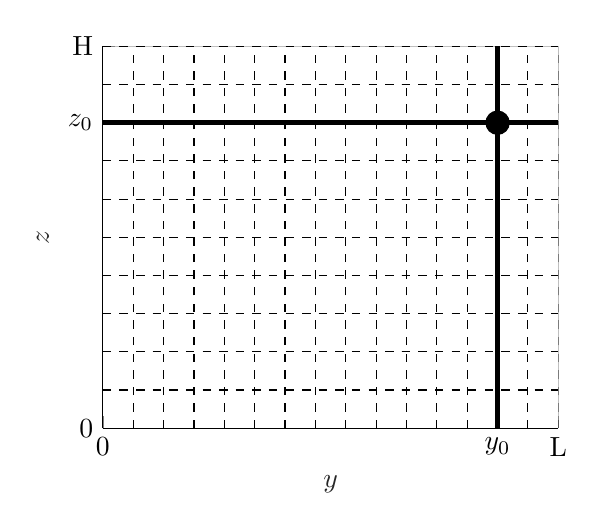
\begin{tikzpicture}

\begin{axis}[%
width=0.477\textwidth,
height=0.4\textwidth,
at={(0\textwidth,0\textwidth)},
scale only axis,
xmin=0,
xmax=15,
xtick={0,13,15},
xticklabels={{0},{$y_0$},{L}},
xlabel style={font=\color{white!15!black}},
xlabel={$y$},
ymin=0,
ymax=5,
ytick={0,4,5},
yticklabels={{0},{$z_0$},{H}},
ylabel style={font=\color{white!15!black}},
ylabel={$z$},
axis background/.style={fill=white},
axis x line*=bottom,
axis y line*=left,
xmajorgrids,
ymajorgrids
]
\addplot [color=black, dashed, forget plot]
  table[row sep=crcr]{%
0	0\\
0	0.0505050505050505\\
0	0.101010101010101\\
0	0.151515151515152\\
0	0.202020202020202\\
0	0.252525252525253\\
0	0.303030303030303\\
0	0.353535353535354\\
0	0.404040404040404\\
0	0.454545454545455\\
0	0.505050505050505\\
0	0.555555555555556\\
0	0.606060606060606\\
0	0.656565656565657\\
0	0.707070707070707\\
0	0.757575757575758\\
0	0.808080808080808\\
0	0.858585858585859\\
0	0.909090909090909\\
0	0.95959595959596\\
0	1.01010101010101\\
0	1.06060606060606\\
0	1.11111111111111\\
0	1.16161616161616\\
0	1.21212121212121\\
0	1.26262626262626\\
0	1.31313131313131\\
0	1.36363636363636\\
0	1.41414141414141\\
0	1.46464646464646\\
0	1.51515151515152\\
0	1.56565656565657\\
0	1.61616161616162\\
0	1.66666666666667\\
0	1.71717171717172\\
0	1.76767676767677\\
0	1.81818181818182\\
0	1.86868686868687\\
0	1.91919191919192\\
0	1.96969696969697\\
0	2.02020202020202\\
0	2.07070707070707\\
0	2.12121212121212\\
0	2.17171717171717\\
0	2.22222222222222\\
0	2.27272727272727\\
0	2.32323232323232\\
0	2.37373737373737\\
0	2.42424242424242\\
0	2.47474747474747\\
0	2.52525252525253\\
0	2.57575757575758\\
0	2.62626262626263\\
0	2.67676767676768\\
0	2.72727272727273\\
0	2.77777777777778\\
0	2.82828282828283\\
0	2.87878787878788\\
0	2.92929292929293\\
0	2.97979797979798\\
0	3.03030303030303\\
0	3.08080808080808\\
0	3.13131313131313\\
0	3.18181818181818\\
0	3.23232323232323\\
0	3.28282828282828\\
0	3.33333333333333\\
0	3.38383838383838\\
0	3.43434343434343\\
0	3.48484848484848\\
0	3.53535353535354\\
0	3.58585858585859\\
0	3.63636363636364\\
0	3.68686868686869\\
0	3.73737373737374\\
0	3.78787878787879\\
0	3.83838383838384\\
0	3.88888888888889\\
0	3.93939393939394\\
0	3.98989898989899\\
0	4.04040404040404\\
0	4.09090909090909\\
0	4.14141414141414\\
0	4.19191919191919\\
0	4.24242424242424\\
0	4.29292929292929\\
0	4.34343434343434\\
0	4.39393939393939\\
0	4.44444444444444\\
0	4.49494949494949\\
0	4.54545454545455\\
0	4.5959595959596\\
0	4.64646464646465\\
0	4.6969696969697\\
0	4.74747474747475\\
0	4.7979797979798\\
0	4.84848484848485\\
0	4.8989898989899\\
0	4.94949494949495\\
0	5\\
};
\addplot [color=black, dashed, forget plot]
  table[row sep=crcr]{%
1	0\\
1	0.0505050505050505\\
1	0.101010101010101\\
1	0.151515151515152\\
1	0.202020202020202\\
1	0.252525252525253\\
1	0.303030303030303\\
1	0.353535353535354\\
1	0.404040404040404\\
1	0.454545454545455\\
1	0.505050505050505\\
1	0.555555555555556\\
1	0.606060606060606\\
1	0.656565656565657\\
1	0.707070707070707\\
1	0.757575757575758\\
1	0.808080808080808\\
1	0.858585858585859\\
1	0.909090909090909\\
1	0.95959595959596\\
1	1.01010101010101\\
1	1.06060606060606\\
1	1.11111111111111\\
1	1.16161616161616\\
1	1.21212121212121\\
1	1.26262626262626\\
1	1.31313131313131\\
1	1.36363636363636\\
1	1.41414141414141\\
1	1.46464646464646\\
1	1.51515151515152\\
1	1.56565656565657\\
1	1.61616161616162\\
1	1.66666666666667\\
1	1.71717171717172\\
1	1.76767676767677\\
1	1.81818181818182\\
1	1.86868686868687\\
1	1.91919191919192\\
1	1.96969696969697\\
1	2.02020202020202\\
1	2.07070707070707\\
1	2.12121212121212\\
1	2.17171717171717\\
1	2.22222222222222\\
1	2.27272727272727\\
1	2.32323232323232\\
1	2.37373737373737\\
1	2.42424242424242\\
1	2.47474747474747\\
1	2.52525252525253\\
1	2.57575757575758\\
1	2.62626262626263\\
1	2.67676767676768\\
1	2.72727272727273\\
1	2.77777777777778\\
1	2.82828282828283\\
1	2.87878787878788\\
1	2.92929292929293\\
1	2.97979797979798\\
1	3.03030303030303\\
1	3.08080808080808\\
1	3.13131313131313\\
1	3.18181818181818\\
1	3.23232323232323\\
1	3.28282828282828\\
1	3.33333333333333\\
1	3.38383838383838\\
1	3.43434343434343\\
1	3.48484848484848\\
1	3.53535353535354\\
1	3.58585858585859\\
1	3.63636363636364\\
1	3.68686868686869\\
1	3.73737373737374\\
1	3.78787878787879\\
1	3.83838383838384\\
1	3.88888888888889\\
1	3.93939393939394\\
1	3.98989898989899\\
1	4.04040404040404\\
1	4.09090909090909\\
1	4.14141414141414\\
1	4.19191919191919\\
1	4.24242424242424\\
1	4.29292929292929\\
1	4.34343434343434\\
1	4.39393939393939\\
1	4.44444444444444\\
1	4.49494949494949\\
1	4.54545454545455\\
1	4.5959595959596\\
1	4.64646464646465\\
1	4.6969696969697\\
1	4.74747474747475\\
1	4.7979797979798\\
1	4.84848484848485\\
1	4.8989898989899\\
1	4.94949494949495\\
1	5\\
};
\addplot [color=black, dashed, forget plot]
  table[row sep=crcr]{%
2	0\\
2	0.0505050505050505\\
2	0.101010101010101\\
2	0.151515151515152\\
2	0.202020202020202\\
2	0.252525252525253\\
2	0.303030303030303\\
2	0.353535353535354\\
2	0.404040404040404\\
2	0.454545454545455\\
2	0.505050505050505\\
2	0.555555555555556\\
2	0.606060606060606\\
2	0.656565656565657\\
2	0.707070707070707\\
2	0.757575757575758\\
2	0.808080808080808\\
2	0.858585858585859\\
2	0.909090909090909\\
2	0.95959595959596\\
2	1.01010101010101\\
2	1.06060606060606\\
2	1.11111111111111\\
2	1.16161616161616\\
2	1.21212121212121\\
2	1.26262626262626\\
2	1.31313131313131\\
2	1.36363636363636\\
2	1.41414141414141\\
2	1.46464646464646\\
2	1.51515151515152\\
2	1.56565656565657\\
2	1.61616161616162\\
2	1.66666666666667\\
2	1.71717171717172\\
2	1.76767676767677\\
2	1.81818181818182\\
2	1.86868686868687\\
2	1.91919191919192\\
2	1.96969696969697\\
2	2.02020202020202\\
2	2.07070707070707\\
2	2.12121212121212\\
2	2.17171717171717\\
2	2.22222222222222\\
2	2.27272727272727\\
2	2.32323232323232\\
2	2.37373737373737\\
2	2.42424242424242\\
2	2.47474747474747\\
2	2.52525252525253\\
2	2.57575757575758\\
2	2.62626262626263\\
2	2.67676767676768\\
2	2.72727272727273\\
2	2.77777777777778\\
2	2.82828282828283\\
2	2.87878787878788\\
2	2.92929292929293\\
2	2.97979797979798\\
2	3.03030303030303\\
2	3.08080808080808\\
2	3.13131313131313\\
2	3.18181818181818\\
2	3.23232323232323\\
2	3.28282828282828\\
2	3.33333333333333\\
2	3.38383838383838\\
2	3.43434343434343\\
2	3.48484848484848\\
2	3.53535353535354\\
2	3.58585858585859\\
2	3.63636363636364\\
2	3.68686868686869\\
2	3.73737373737374\\
2	3.78787878787879\\
2	3.83838383838384\\
2	3.88888888888889\\
2	3.93939393939394\\
2	3.98989898989899\\
2	4.04040404040404\\
2	4.09090909090909\\
2	4.14141414141414\\
2	4.19191919191919\\
2	4.24242424242424\\
2	4.29292929292929\\
2	4.34343434343434\\
2	4.39393939393939\\
2	4.44444444444444\\
2	4.49494949494949\\
2	4.54545454545455\\
2	4.5959595959596\\
2	4.64646464646465\\
2	4.6969696969697\\
2	4.74747474747475\\
2	4.7979797979798\\
2	4.84848484848485\\
2	4.8989898989899\\
2	4.94949494949495\\
2	5\\
};
\addplot [color=black, dashed, forget plot]
  table[row sep=crcr]{%
3	0\\
3	0.0505050505050505\\
3	0.101010101010101\\
3	0.151515151515152\\
3	0.202020202020202\\
3	0.252525252525253\\
3	0.303030303030303\\
3	0.353535353535354\\
3	0.404040404040404\\
3	0.454545454545455\\
3	0.505050505050505\\
3	0.555555555555556\\
3	0.606060606060606\\
3	0.656565656565657\\
3	0.707070707070707\\
3	0.757575757575758\\
3	0.808080808080808\\
3	0.858585858585859\\
3	0.909090909090909\\
3	0.95959595959596\\
3	1.01010101010101\\
3	1.06060606060606\\
3	1.11111111111111\\
3	1.16161616161616\\
3	1.21212121212121\\
3	1.26262626262626\\
3	1.31313131313131\\
3	1.36363636363636\\
3	1.41414141414141\\
3	1.46464646464646\\
3	1.51515151515152\\
3	1.56565656565657\\
3	1.61616161616162\\
3	1.66666666666667\\
3	1.71717171717172\\
3	1.76767676767677\\
3	1.81818181818182\\
3	1.86868686868687\\
3	1.91919191919192\\
3	1.96969696969697\\
3	2.02020202020202\\
3	2.07070707070707\\
3	2.12121212121212\\
3	2.17171717171717\\
3	2.22222222222222\\
3	2.27272727272727\\
3	2.32323232323232\\
3	2.37373737373737\\
3	2.42424242424242\\
3	2.47474747474747\\
3	2.52525252525253\\
3	2.57575757575758\\
3	2.62626262626263\\
3	2.67676767676768\\
3	2.72727272727273\\
3	2.77777777777778\\
3	2.82828282828283\\
3	2.87878787878788\\
3	2.92929292929293\\
3	2.97979797979798\\
3	3.03030303030303\\
3	3.08080808080808\\
3	3.13131313131313\\
3	3.18181818181818\\
3	3.23232323232323\\
3	3.28282828282828\\
3	3.33333333333333\\
3	3.38383838383838\\
3	3.43434343434343\\
3	3.48484848484848\\
3	3.53535353535354\\
3	3.58585858585859\\
3	3.63636363636364\\
3	3.68686868686869\\
3	3.73737373737374\\
3	3.78787878787879\\
3	3.83838383838384\\
3	3.88888888888889\\
3	3.93939393939394\\
3	3.98989898989899\\
3	4.04040404040404\\
3	4.09090909090909\\
3	4.14141414141414\\
3	4.19191919191919\\
3	4.24242424242424\\
3	4.29292929292929\\
3	4.34343434343434\\
3	4.39393939393939\\
3	4.44444444444444\\
3	4.49494949494949\\
3	4.54545454545455\\
3	4.5959595959596\\
3	4.64646464646465\\
3	4.6969696969697\\
3	4.74747474747475\\
3	4.7979797979798\\
3	4.84848484848485\\
3	4.8989898989899\\
3	4.94949494949495\\
3	5\\
};
\addplot [color=black, dashed, forget plot]
  table[row sep=crcr]{%
4	0\\
4	0.0505050505050505\\
4	0.101010101010101\\
4	0.151515151515152\\
4	0.202020202020202\\
4	0.252525252525253\\
4	0.303030303030303\\
4	0.353535353535354\\
4	0.404040404040404\\
4	0.454545454545455\\
4	0.505050505050505\\
4	0.555555555555556\\
4	0.606060606060606\\
4	0.656565656565657\\
4	0.707070707070707\\
4	0.757575757575758\\
4	0.808080808080808\\
4	0.858585858585859\\
4	0.909090909090909\\
4	0.95959595959596\\
4	1.01010101010101\\
4	1.06060606060606\\
4	1.11111111111111\\
4	1.16161616161616\\
4	1.21212121212121\\
4	1.26262626262626\\
4	1.31313131313131\\
4	1.36363636363636\\
4	1.41414141414141\\
4	1.46464646464646\\
4	1.51515151515152\\
4	1.56565656565657\\
4	1.61616161616162\\
4	1.66666666666667\\
4	1.71717171717172\\
4	1.76767676767677\\
4	1.81818181818182\\
4	1.86868686868687\\
4	1.91919191919192\\
4	1.96969696969697\\
4	2.02020202020202\\
4	2.07070707070707\\
4	2.12121212121212\\
4	2.17171717171717\\
4	2.22222222222222\\
4	2.27272727272727\\
4	2.32323232323232\\
4	2.37373737373737\\
4	2.42424242424242\\
4	2.47474747474747\\
4	2.52525252525253\\
4	2.57575757575758\\
4	2.62626262626263\\
4	2.67676767676768\\
4	2.72727272727273\\
4	2.77777777777778\\
4	2.82828282828283\\
4	2.87878787878788\\
4	2.92929292929293\\
4	2.97979797979798\\
4	3.03030303030303\\
4	3.08080808080808\\
4	3.13131313131313\\
4	3.18181818181818\\
4	3.23232323232323\\
4	3.28282828282828\\
4	3.33333333333333\\
4	3.38383838383838\\
4	3.43434343434343\\
4	3.48484848484848\\
4	3.53535353535354\\
4	3.58585858585859\\
4	3.63636363636364\\
4	3.68686868686869\\
4	3.73737373737374\\
4	3.78787878787879\\
4	3.83838383838384\\
4	3.88888888888889\\
4	3.93939393939394\\
4	3.98989898989899\\
4	4.04040404040404\\
4	4.09090909090909\\
4	4.14141414141414\\
4	4.19191919191919\\
4	4.24242424242424\\
4	4.29292929292929\\
4	4.34343434343434\\
4	4.39393939393939\\
4	4.44444444444444\\
4	4.49494949494949\\
4	4.54545454545455\\
4	4.5959595959596\\
4	4.64646464646465\\
4	4.6969696969697\\
4	4.74747474747475\\
4	4.7979797979798\\
4	4.84848484848485\\
4	4.8989898989899\\
4	4.94949494949495\\
4	5\\
};
\addplot [color=black, dashed, forget plot]
  table[row sep=crcr]{%
5	0\\
5	0.0505050505050505\\
5	0.101010101010101\\
5	0.151515151515152\\
5	0.202020202020202\\
5	0.252525252525253\\
5	0.303030303030303\\
5	0.353535353535354\\
5	0.404040404040404\\
5	0.454545454545455\\
5	0.505050505050505\\
5	0.555555555555556\\
5	0.606060606060606\\
5	0.656565656565657\\
5	0.707070707070707\\
5	0.757575757575758\\
5	0.808080808080808\\
5	0.858585858585859\\
5	0.909090909090909\\
5	0.95959595959596\\
5	1.01010101010101\\
5	1.06060606060606\\
5	1.11111111111111\\
5	1.16161616161616\\
5	1.21212121212121\\
5	1.26262626262626\\
5	1.31313131313131\\
5	1.36363636363636\\
5	1.41414141414141\\
5	1.46464646464646\\
5	1.51515151515152\\
5	1.56565656565657\\
5	1.61616161616162\\
5	1.66666666666667\\
5	1.71717171717172\\
5	1.76767676767677\\
5	1.81818181818182\\
5	1.86868686868687\\
5	1.91919191919192\\
5	1.96969696969697\\
5	2.02020202020202\\
5	2.07070707070707\\
5	2.12121212121212\\
5	2.17171717171717\\
5	2.22222222222222\\
5	2.27272727272727\\
5	2.32323232323232\\
5	2.37373737373737\\
5	2.42424242424242\\
5	2.47474747474747\\
5	2.52525252525253\\
5	2.57575757575758\\
5	2.62626262626263\\
5	2.67676767676768\\
5	2.72727272727273\\
5	2.77777777777778\\
5	2.82828282828283\\
5	2.87878787878788\\
5	2.92929292929293\\
5	2.97979797979798\\
5	3.03030303030303\\
5	3.08080808080808\\
5	3.13131313131313\\
5	3.18181818181818\\
5	3.23232323232323\\
5	3.28282828282828\\
5	3.33333333333333\\
5	3.38383838383838\\
5	3.43434343434343\\
5	3.48484848484848\\
5	3.53535353535354\\
5	3.58585858585859\\
5	3.63636363636364\\
5	3.68686868686869\\
5	3.73737373737374\\
5	3.78787878787879\\
5	3.83838383838384\\
5	3.88888888888889\\
5	3.93939393939394\\
5	3.98989898989899\\
5	4.04040404040404\\
5	4.09090909090909\\
5	4.14141414141414\\
5	4.19191919191919\\
5	4.24242424242424\\
5	4.29292929292929\\
5	4.34343434343434\\
5	4.39393939393939\\
5	4.44444444444444\\
5	4.49494949494949\\
5	4.54545454545455\\
5	4.5959595959596\\
5	4.64646464646465\\
5	4.6969696969697\\
5	4.74747474747475\\
5	4.7979797979798\\
5	4.84848484848485\\
5	4.8989898989899\\
5	4.94949494949495\\
5	5\\
};
\addplot [color=black, dashed, forget plot]
  table[row sep=crcr]{%
6	0\\
6	0.0505050505050505\\
6	0.101010101010101\\
6	0.151515151515152\\
6	0.202020202020202\\
6	0.252525252525253\\
6	0.303030303030303\\
6	0.353535353535354\\
6	0.404040404040404\\
6	0.454545454545455\\
6	0.505050505050505\\
6	0.555555555555556\\
6	0.606060606060606\\
6	0.656565656565657\\
6	0.707070707070707\\
6	0.757575757575758\\
6	0.808080808080808\\
6	0.858585858585859\\
6	0.909090909090909\\
6	0.95959595959596\\
6	1.01010101010101\\
6	1.06060606060606\\
6	1.11111111111111\\
6	1.16161616161616\\
6	1.21212121212121\\
6	1.26262626262626\\
6	1.31313131313131\\
6	1.36363636363636\\
6	1.41414141414141\\
6	1.46464646464646\\
6	1.51515151515152\\
6	1.56565656565657\\
6	1.61616161616162\\
6	1.66666666666667\\
6	1.71717171717172\\
6	1.76767676767677\\
6	1.81818181818182\\
6	1.86868686868687\\
6	1.91919191919192\\
6	1.96969696969697\\
6	2.02020202020202\\
6	2.07070707070707\\
6	2.12121212121212\\
6	2.17171717171717\\
6	2.22222222222222\\
6	2.27272727272727\\
6	2.32323232323232\\
6	2.37373737373737\\
6	2.42424242424242\\
6	2.47474747474747\\
6	2.52525252525253\\
6	2.57575757575758\\
6	2.62626262626263\\
6	2.67676767676768\\
6	2.72727272727273\\
6	2.77777777777778\\
6	2.82828282828283\\
6	2.87878787878788\\
6	2.92929292929293\\
6	2.97979797979798\\
6	3.03030303030303\\
6	3.08080808080808\\
6	3.13131313131313\\
6	3.18181818181818\\
6	3.23232323232323\\
6	3.28282828282828\\
6	3.33333333333333\\
6	3.38383838383838\\
6	3.43434343434343\\
6	3.48484848484848\\
6	3.53535353535354\\
6	3.58585858585859\\
6	3.63636363636364\\
6	3.68686868686869\\
6	3.73737373737374\\
6	3.78787878787879\\
6	3.83838383838384\\
6	3.88888888888889\\
6	3.93939393939394\\
6	3.98989898989899\\
6	4.04040404040404\\
6	4.09090909090909\\
6	4.14141414141414\\
6	4.19191919191919\\
6	4.24242424242424\\
6	4.29292929292929\\
6	4.34343434343434\\
6	4.39393939393939\\
6	4.44444444444444\\
6	4.49494949494949\\
6	4.54545454545455\\
6	4.5959595959596\\
6	4.64646464646465\\
6	4.6969696969697\\
6	4.74747474747475\\
6	4.7979797979798\\
6	4.84848484848485\\
6	4.8989898989899\\
6	4.94949494949495\\
6	5\\
};
\addplot [color=black, dashed, forget plot]
  table[row sep=crcr]{%
7	0\\
7	0.0505050505050505\\
7	0.101010101010101\\
7	0.151515151515152\\
7	0.202020202020202\\
7	0.252525252525253\\
7	0.303030303030303\\
7	0.353535353535354\\
7	0.404040404040404\\
7	0.454545454545455\\
7	0.505050505050505\\
7	0.555555555555556\\
7	0.606060606060606\\
7	0.656565656565657\\
7	0.707070707070707\\
7	0.757575757575758\\
7	0.808080808080808\\
7	0.858585858585859\\
7	0.909090909090909\\
7	0.95959595959596\\
7	1.01010101010101\\
7	1.06060606060606\\
7	1.11111111111111\\
7	1.16161616161616\\
7	1.21212121212121\\
7	1.26262626262626\\
7	1.31313131313131\\
7	1.36363636363636\\
7	1.41414141414141\\
7	1.46464646464646\\
7	1.51515151515152\\
7	1.56565656565657\\
7	1.61616161616162\\
7	1.66666666666667\\
7	1.71717171717172\\
7	1.76767676767677\\
7	1.81818181818182\\
7	1.86868686868687\\
7	1.91919191919192\\
7	1.96969696969697\\
7	2.02020202020202\\
7	2.07070707070707\\
7	2.12121212121212\\
7	2.17171717171717\\
7	2.22222222222222\\
7	2.27272727272727\\
7	2.32323232323232\\
7	2.37373737373737\\
7	2.42424242424242\\
7	2.47474747474747\\
7	2.52525252525253\\
7	2.57575757575758\\
7	2.62626262626263\\
7	2.67676767676768\\
7	2.72727272727273\\
7	2.77777777777778\\
7	2.82828282828283\\
7	2.87878787878788\\
7	2.92929292929293\\
7	2.97979797979798\\
7	3.03030303030303\\
7	3.08080808080808\\
7	3.13131313131313\\
7	3.18181818181818\\
7	3.23232323232323\\
7	3.28282828282828\\
7	3.33333333333333\\
7	3.38383838383838\\
7	3.43434343434343\\
7	3.48484848484848\\
7	3.53535353535354\\
7	3.58585858585859\\
7	3.63636363636364\\
7	3.68686868686869\\
7	3.73737373737374\\
7	3.78787878787879\\
7	3.83838383838384\\
7	3.88888888888889\\
7	3.93939393939394\\
7	3.98989898989899\\
7	4.04040404040404\\
7	4.09090909090909\\
7	4.14141414141414\\
7	4.19191919191919\\
7	4.24242424242424\\
7	4.29292929292929\\
7	4.34343434343434\\
7	4.39393939393939\\
7	4.44444444444444\\
7	4.49494949494949\\
7	4.54545454545455\\
7	4.5959595959596\\
7	4.64646464646465\\
7	4.6969696969697\\
7	4.74747474747475\\
7	4.7979797979798\\
7	4.84848484848485\\
7	4.8989898989899\\
7	4.94949494949495\\
7	5\\
};
\addplot [color=black, dashed, forget plot]
  table[row sep=crcr]{%
8	0\\
8	0.0505050505050505\\
8	0.101010101010101\\
8	0.151515151515152\\
8	0.202020202020202\\
8	0.252525252525253\\
8	0.303030303030303\\
8	0.353535353535354\\
8	0.404040404040404\\
8	0.454545454545455\\
8	0.505050505050505\\
8	0.555555555555556\\
8	0.606060606060606\\
8	0.656565656565657\\
8	0.707070707070707\\
8	0.757575757575758\\
8	0.808080808080808\\
8	0.858585858585859\\
8	0.909090909090909\\
8	0.95959595959596\\
8	1.01010101010101\\
8	1.06060606060606\\
8	1.11111111111111\\
8	1.16161616161616\\
8	1.21212121212121\\
8	1.26262626262626\\
8	1.31313131313131\\
8	1.36363636363636\\
8	1.41414141414141\\
8	1.46464646464646\\
8	1.51515151515152\\
8	1.56565656565657\\
8	1.61616161616162\\
8	1.66666666666667\\
8	1.71717171717172\\
8	1.76767676767677\\
8	1.81818181818182\\
8	1.86868686868687\\
8	1.91919191919192\\
8	1.96969696969697\\
8	2.02020202020202\\
8	2.07070707070707\\
8	2.12121212121212\\
8	2.17171717171717\\
8	2.22222222222222\\
8	2.27272727272727\\
8	2.32323232323232\\
8	2.37373737373737\\
8	2.42424242424242\\
8	2.47474747474747\\
8	2.52525252525253\\
8	2.57575757575758\\
8	2.62626262626263\\
8	2.67676767676768\\
8	2.72727272727273\\
8	2.77777777777778\\
8	2.82828282828283\\
8	2.87878787878788\\
8	2.92929292929293\\
8	2.97979797979798\\
8	3.03030303030303\\
8	3.08080808080808\\
8	3.13131313131313\\
8	3.18181818181818\\
8	3.23232323232323\\
8	3.28282828282828\\
8	3.33333333333333\\
8	3.38383838383838\\
8	3.43434343434343\\
8	3.48484848484848\\
8	3.53535353535354\\
8	3.58585858585859\\
8	3.63636363636364\\
8	3.68686868686869\\
8	3.73737373737374\\
8	3.78787878787879\\
8	3.83838383838384\\
8	3.88888888888889\\
8	3.93939393939394\\
8	3.98989898989899\\
8	4.04040404040404\\
8	4.09090909090909\\
8	4.14141414141414\\
8	4.19191919191919\\
8	4.24242424242424\\
8	4.29292929292929\\
8	4.34343434343434\\
8	4.39393939393939\\
8	4.44444444444444\\
8	4.49494949494949\\
8	4.54545454545455\\
8	4.5959595959596\\
8	4.64646464646465\\
8	4.6969696969697\\
8	4.74747474747475\\
8	4.7979797979798\\
8	4.84848484848485\\
8	4.8989898989899\\
8	4.94949494949495\\
8	5\\
};
\addplot [color=black, dashed, forget plot]
  table[row sep=crcr]{%
9	0\\
9	0.0505050505050505\\
9	0.101010101010101\\
9	0.151515151515152\\
9	0.202020202020202\\
9	0.252525252525253\\
9	0.303030303030303\\
9	0.353535353535354\\
9	0.404040404040404\\
9	0.454545454545455\\
9	0.505050505050505\\
9	0.555555555555556\\
9	0.606060606060606\\
9	0.656565656565657\\
9	0.707070707070707\\
9	0.757575757575758\\
9	0.808080808080808\\
9	0.858585858585859\\
9	0.909090909090909\\
9	0.95959595959596\\
9	1.01010101010101\\
9	1.06060606060606\\
9	1.11111111111111\\
9	1.16161616161616\\
9	1.21212121212121\\
9	1.26262626262626\\
9	1.31313131313131\\
9	1.36363636363636\\
9	1.41414141414141\\
9	1.46464646464646\\
9	1.51515151515152\\
9	1.56565656565657\\
9	1.61616161616162\\
9	1.66666666666667\\
9	1.71717171717172\\
9	1.76767676767677\\
9	1.81818181818182\\
9	1.86868686868687\\
9	1.91919191919192\\
9	1.96969696969697\\
9	2.02020202020202\\
9	2.07070707070707\\
9	2.12121212121212\\
9	2.17171717171717\\
9	2.22222222222222\\
9	2.27272727272727\\
9	2.32323232323232\\
9	2.37373737373737\\
9	2.42424242424242\\
9	2.47474747474747\\
9	2.52525252525253\\
9	2.57575757575758\\
9	2.62626262626263\\
9	2.67676767676768\\
9	2.72727272727273\\
9	2.77777777777778\\
9	2.82828282828283\\
9	2.87878787878788\\
9	2.92929292929293\\
9	2.97979797979798\\
9	3.03030303030303\\
9	3.08080808080808\\
9	3.13131313131313\\
9	3.18181818181818\\
9	3.23232323232323\\
9	3.28282828282828\\
9	3.33333333333333\\
9	3.38383838383838\\
9	3.43434343434343\\
9	3.48484848484848\\
9	3.53535353535354\\
9	3.58585858585859\\
9	3.63636363636364\\
9	3.68686868686869\\
9	3.73737373737374\\
9	3.78787878787879\\
9	3.83838383838384\\
9	3.88888888888889\\
9	3.93939393939394\\
9	3.98989898989899\\
9	4.04040404040404\\
9	4.09090909090909\\
9	4.14141414141414\\
9	4.19191919191919\\
9	4.24242424242424\\
9	4.29292929292929\\
9	4.34343434343434\\
9	4.39393939393939\\
9	4.44444444444444\\
9	4.49494949494949\\
9	4.54545454545455\\
9	4.5959595959596\\
9	4.64646464646465\\
9	4.6969696969697\\
9	4.74747474747475\\
9	4.7979797979798\\
9	4.84848484848485\\
9	4.8989898989899\\
9	4.94949494949495\\
9	5\\
};
\addplot [color=black, dashed, forget plot]
  table[row sep=crcr]{%
10	0\\
10	0.0505050505050505\\
10	0.101010101010101\\
10	0.151515151515152\\
10	0.202020202020202\\
10	0.252525252525253\\
10	0.303030303030303\\
10	0.353535353535354\\
10	0.404040404040404\\
10	0.454545454545455\\
10	0.505050505050505\\
10	0.555555555555556\\
10	0.606060606060606\\
10	0.656565656565657\\
10	0.707070707070707\\
10	0.757575757575758\\
10	0.808080808080808\\
10	0.858585858585859\\
10	0.909090909090909\\
10	0.95959595959596\\
10	1.01010101010101\\
10	1.06060606060606\\
10	1.11111111111111\\
10	1.16161616161616\\
10	1.21212121212121\\
10	1.26262626262626\\
10	1.31313131313131\\
10	1.36363636363636\\
10	1.41414141414141\\
10	1.46464646464646\\
10	1.51515151515152\\
10	1.56565656565657\\
10	1.61616161616162\\
10	1.66666666666667\\
10	1.71717171717172\\
10	1.76767676767677\\
10	1.81818181818182\\
10	1.86868686868687\\
10	1.91919191919192\\
10	1.96969696969697\\
10	2.02020202020202\\
10	2.07070707070707\\
10	2.12121212121212\\
10	2.17171717171717\\
10	2.22222222222222\\
10	2.27272727272727\\
10	2.32323232323232\\
10	2.37373737373737\\
10	2.42424242424242\\
10	2.47474747474747\\
10	2.52525252525253\\
10	2.57575757575758\\
10	2.62626262626263\\
10	2.67676767676768\\
10	2.72727272727273\\
10	2.77777777777778\\
10	2.82828282828283\\
10	2.87878787878788\\
10	2.92929292929293\\
10	2.97979797979798\\
10	3.03030303030303\\
10	3.08080808080808\\
10	3.13131313131313\\
10	3.18181818181818\\
10	3.23232323232323\\
10	3.28282828282828\\
10	3.33333333333333\\
10	3.38383838383838\\
10	3.43434343434343\\
10	3.48484848484848\\
10	3.53535353535354\\
10	3.58585858585859\\
10	3.63636363636364\\
10	3.68686868686869\\
10	3.73737373737374\\
10	3.78787878787879\\
10	3.83838383838384\\
10	3.88888888888889\\
10	3.93939393939394\\
10	3.98989898989899\\
10	4.04040404040404\\
10	4.09090909090909\\
10	4.14141414141414\\
10	4.19191919191919\\
10	4.24242424242424\\
10	4.29292929292929\\
10	4.34343434343434\\
10	4.39393939393939\\
10	4.44444444444444\\
10	4.49494949494949\\
10	4.54545454545455\\
10	4.5959595959596\\
10	4.64646464646465\\
10	4.6969696969697\\
10	4.74747474747475\\
10	4.7979797979798\\
10	4.84848484848485\\
10	4.8989898989899\\
10	4.94949494949495\\
10	5\\
};
\addplot [color=black, dashed, forget plot]
  table[row sep=crcr]{%
11	0\\
11	0.0505050505050505\\
11	0.101010101010101\\
11	0.151515151515152\\
11	0.202020202020202\\
11	0.252525252525253\\
11	0.303030303030303\\
11	0.353535353535354\\
11	0.404040404040404\\
11	0.454545454545455\\
11	0.505050505050505\\
11	0.555555555555556\\
11	0.606060606060606\\
11	0.656565656565657\\
11	0.707070707070707\\
11	0.757575757575758\\
11	0.808080808080808\\
11	0.858585858585859\\
11	0.909090909090909\\
11	0.95959595959596\\
11	1.01010101010101\\
11	1.06060606060606\\
11	1.11111111111111\\
11	1.16161616161616\\
11	1.21212121212121\\
11	1.26262626262626\\
11	1.31313131313131\\
11	1.36363636363636\\
11	1.41414141414141\\
11	1.46464646464646\\
11	1.51515151515152\\
11	1.56565656565657\\
11	1.61616161616162\\
11	1.66666666666667\\
11	1.71717171717172\\
11	1.76767676767677\\
11	1.81818181818182\\
11	1.86868686868687\\
11	1.91919191919192\\
11	1.96969696969697\\
11	2.02020202020202\\
11	2.07070707070707\\
11	2.12121212121212\\
11	2.17171717171717\\
11	2.22222222222222\\
11	2.27272727272727\\
11	2.32323232323232\\
11	2.37373737373737\\
11	2.42424242424242\\
11	2.47474747474747\\
11	2.52525252525253\\
11	2.57575757575758\\
11	2.62626262626263\\
11	2.67676767676768\\
11	2.72727272727273\\
11	2.77777777777778\\
11	2.82828282828283\\
11	2.87878787878788\\
11	2.92929292929293\\
11	2.97979797979798\\
11	3.03030303030303\\
11	3.08080808080808\\
11	3.13131313131313\\
11	3.18181818181818\\
11	3.23232323232323\\
11	3.28282828282828\\
11	3.33333333333333\\
11	3.38383838383838\\
11	3.43434343434343\\
11	3.48484848484848\\
11	3.53535353535354\\
11	3.58585858585859\\
11	3.63636363636364\\
11	3.68686868686869\\
11	3.73737373737374\\
11	3.78787878787879\\
11	3.83838383838384\\
11	3.88888888888889\\
11	3.93939393939394\\
11	3.98989898989899\\
11	4.04040404040404\\
11	4.09090909090909\\
11	4.14141414141414\\
11	4.19191919191919\\
11	4.24242424242424\\
11	4.29292929292929\\
11	4.34343434343434\\
11	4.39393939393939\\
11	4.44444444444444\\
11	4.49494949494949\\
11	4.54545454545455\\
11	4.5959595959596\\
11	4.64646464646465\\
11	4.6969696969697\\
11	4.74747474747475\\
11	4.7979797979798\\
11	4.84848484848485\\
11	4.8989898989899\\
11	4.94949494949495\\
11	5\\
};
\addplot [color=black, dashed, forget plot]
  table[row sep=crcr]{%
12	0\\
12	0.0505050505050505\\
12	0.101010101010101\\
12	0.151515151515152\\
12	0.202020202020202\\
12	0.252525252525253\\
12	0.303030303030303\\
12	0.353535353535354\\
12	0.404040404040404\\
12	0.454545454545455\\
12	0.505050505050505\\
12	0.555555555555556\\
12	0.606060606060606\\
12	0.656565656565657\\
12	0.707070707070707\\
12	0.757575757575758\\
12	0.808080808080808\\
12	0.858585858585859\\
12	0.909090909090909\\
12	0.95959595959596\\
12	1.01010101010101\\
12	1.06060606060606\\
12	1.11111111111111\\
12	1.16161616161616\\
12	1.21212121212121\\
12	1.26262626262626\\
12	1.31313131313131\\
12	1.36363636363636\\
12	1.41414141414141\\
12	1.46464646464646\\
12	1.51515151515152\\
12	1.56565656565657\\
12	1.61616161616162\\
12	1.66666666666667\\
12	1.71717171717172\\
12	1.76767676767677\\
12	1.81818181818182\\
12	1.86868686868687\\
12	1.91919191919192\\
12	1.96969696969697\\
12	2.02020202020202\\
12	2.07070707070707\\
12	2.12121212121212\\
12	2.17171717171717\\
12	2.22222222222222\\
12	2.27272727272727\\
12	2.32323232323232\\
12	2.37373737373737\\
12	2.42424242424242\\
12	2.47474747474747\\
12	2.52525252525253\\
12	2.57575757575758\\
12	2.62626262626263\\
12	2.67676767676768\\
12	2.72727272727273\\
12	2.77777777777778\\
12	2.82828282828283\\
12	2.87878787878788\\
12	2.92929292929293\\
12	2.97979797979798\\
12	3.03030303030303\\
12	3.08080808080808\\
12	3.13131313131313\\
12	3.18181818181818\\
12	3.23232323232323\\
12	3.28282828282828\\
12	3.33333333333333\\
12	3.38383838383838\\
12	3.43434343434343\\
12	3.48484848484848\\
12	3.53535353535354\\
12	3.58585858585859\\
12	3.63636363636364\\
12	3.68686868686869\\
12	3.73737373737374\\
12	3.78787878787879\\
12	3.83838383838384\\
12	3.88888888888889\\
12	3.93939393939394\\
12	3.98989898989899\\
12	4.04040404040404\\
12	4.09090909090909\\
12	4.14141414141414\\
12	4.19191919191919\\
12	4.24242424242424\\
12	4.29292929292929\\
12	4.34343434343434\\
12	4.39393939393939\\
12	4.44444444444444\\
12	4.49494949494949\\
12	4.54545454545455\\
12	4.5959595959596\\
12	4.64646464646465\\
12	4.6969696969697\\
12	4.74747474747475\\
12	4.7979797979798\\
12	4.84848484848485\\
12	4.8989898989899\\
12	4.94949494949495\\
12	5\\
};
\addplot [color=black, dashed, forget plot]
  table[row sep=crcr]{%
13	0\\
13	0.0505050505050505\\
13	0.101010101010101\\
13	0.151515151515152\\
13	0.202020202020202\\
13	0.252525252525253\\
13	0.303030303030303\\
13	0.353535353535354\\
13	0.404040404040404\\
13	0.454545454545455\\
13	0.505050505050505\\
13	0.555555555555556\\
13	0.606060606060606\\
13	0.656565656565657\\
13	0.707070707070707\\
13	0.757575757575758\\
13	0.808080808080808\\
13	0.858585858585859\\
13	0.909090909090909\\
13	0.95959595959596\\
13	1.01010101010101\\
13	1.06060606060606\\
13	1.11111111111111\\
13	1.16161616161616\\
13	1.21212121212121\\
13	1.26262626262626\\
13	1.31313131313131\\
13	1.36363636363636\\
13	1.41414141414141\\
13	1.46464646464646\\
13	1.51515151515152\\
13	1.56565656565657\\
13	1.61616161616162\\
13	1.66666666666667\\
13	1.71717171717172\\
13	1.76767676767677\\
13	1.81818181818182\\
13	1.86868686868687\\
13	1.91919191919192\\
13	1.96969696969697\\
13	2.02020202020202\\
13	2.07070707070707\\
13	2.12121212121212\\
13	2.17171717171717\\
13	2.22222222222222\\
13	2.27272727272727\\
13	2.32323232323232\\
13	2.37373737373737\\
13	2.42424242424242\\
13	2.47474747474747\\
13	2.52525252525253\\
13	2.57575757575758\\
13	2.62626262626263\\
13	2.67676767676768\\
13	2.72727272727273\\
13	2.77777777777778\\
13	2.82828282828283\\
13	2.87878787878788\\
13	2.92929292929293\\
13	2.97979797979798\\
13	3.03030303030303\\
13	3.08080808080808\\
13	3.13131313131313\\
13	3.18181818181818\\
13	3.23232323232323\\
13	3.28282828282828\\
13	3.33333333333333\\
13	3.38383838383838\\
13	3.43434343434343\\
13	3.48484848484848\\
13	3.53535353535354\\
13	3.58585858585859\\
13	3.63636363636364\\
13	3.68686868686869\\
13	3.73737373737374\\
13	3.78787878787879\\
13	3.83838383838384\\
13	3.88888888888889\\
13	3.93939393939394\\
13	3.98989898989899\\
13	4.04040404040404\\
13	4.09090909090909\\
13	4.14141414141414\\
13	4.19191919191919\\
13	4.24242424242424\\
13	4.29292929292929\\
13	4.34343434343434\\
13	4.39393939393939\\
13	4.44444444444444\\
13	4.49494949494949\\
13	4.54545454545455\\
13	4.5959595959596\\
13	4.64646464646465\\
13	4.6969696969697\\
13	4.74747474747475\\
13	4.7979797979798\\
13	4.84848484848485\\
13	4.8989898989899\\
13	4.94949494949495\\
13	5\\
};
\addplot [color=black, dashed, forget plot]
  table[row sep=crcr]{%
14	0\\
14	0.0505050505050505\\
14	0.101010101010101\\
14	0.151515151515152\\
14	0.202020202020202\\
14	0.252525252525253\\
14	0.303030303030303\\
14	0.353535353535354\\
14	0.404040404040404\\
14	0.454545454545455\\
14	0.505050505050505\\
14	0.555555555555556\\
14	0.606060606060606\\
14	0.656565656565657\\
14	0.707070707070707\\
14	0.757575757575758\\
14	0.808080808080808\\
14	0.858585858585859\\
14	0.909090909090909\\
14	0.95959595959596\\
14	1.01010101010101\\
14	1.06060606060606\\
14	1.11111111111111\\
14	1.16161616161616\\
14	1.21212121212121\\
14	1.26262626262626\\
14	1.31313131313131\\
14	1.36363636363636\\
14	1.41414141414141\\
14	1.46464646464646\\
14	1.51515151515152\\
14	1.56565656565657\\
14	1.61616161616162\\
14	1.66666666666667\\
14	1.71717171717172\\
14	1.76767676767677\\
14	1.81818181818182\\
14	1.86868686868687\\
14	1.91919191919192\\
14	1.96969696969697\\
14	2.02020202020202\\
14	2.07070707070707\\
14	2.12121212121212\\
14	2.17171717171717\\
14	2.22222222222222\\
14	2.27272727272727\\
14	2.32323232323232\\
14	2.37373737373737\\
14	2.42424242424242\\
14	2.47474747474747\\
14	2.52525252525253\\
14	2.57575757575758\\
14	2.62626262626263\\
14	2.67676767676768\\
14	2.72727272727273\\
14	2.77777777777778\\
14	2.82828282828283\\
14	2.87878787878788\\
14	2.92929292929293\\
14	2.97979797979798\\
14	3.03030303030303\\
14	3.08080808080808\\
14	3.13131313131313\\
14	3.18181818181818\\
14	3.23232323232323\\
14	3.28282828282828\\
14	3.33333333333333\\
14	3.38383838383838\\
14	3.43434343434343\\
14	3.48484848484848\\
14	3.53535353535354\\
14	3.58585858585859\\
14	3.63636363636364\\
14	3.68686868686869\\
14	3.73737373737374\\
14	3.78787878787879\\
14	3.83838383838384\\
14	3.88888888888889\\
14	3.93939393939394\\
14	3.98989898989899\\
14	4.04040404040404\\
14	4.09090909090909\\
14	4.14141414141414\\
14	4.19191919191919\\
14	4.24242424242424\\
14	4.29292929292929\\
14	4.34343434343434\\
14	4.39393939393939\\
14	4.44444444444444\\
14	4.49494949494949\\
14	4.54545454545455\\
14	4.5959595959596\\
14	4.64646464646465\\
14	4.6969696969697\\
14	4.74747474747475\\
14	4.7979797979798\\
14	4.84848484848485\\
14	4.8989898989899\\
14	4.94949494949495\\
14	5\\
};
\addplot [color=black, dashed, forget plot]
  table[row sep=crcr]{%
15	0\\
15	0.0505050505050505\\
15	0.101010101010101\\
15	0.151515151515152\\
15	0.202020202020202\\
15	0.252525252525253\\
15	0.303030303030303\\
15	0.353535353535354\\
15	0.404040404040404\\
15	0.454545454545455\\
15	0.505050505050505\\
15	0.555555555555556\\
15	0.606060606060606\\
15	0.656565656565657\\
15	0.707070707070707\\
15	0.757575757575758\\
15	0.808080808080808\\
15	0.858585858585859\\
15	0.909090909090909\\
15	0.95959595959596\\
15	1.01010101010101\\
15	1.06060606060606\\
15	1.11111111111111\\
15	1.16161616161616\\
15	1.21212121212121\\
15	1.26262626262626\\
15	1.31313131313131\\
15	1.36363636363636\\
15	1.41414141414141\\
15	1.46464646464646\\
15	1.51515151515152\\
15	1.56565656565657\\
15	1.61616161616162\\
15	1.66666666666667\\
15	1.71717171717172\\
15	1.76767676767677\\
15	1.81818181818182\\
15	1.86868686868687\\
15	1.91919191919192\\
15	1.96969696969697\\
15	2.02020202020202\\
15	2.07070707070707\\
15	2.12121212121212\\
15	2.17171717171717\\
15	2.22222222222222\\
15	2.27272727272727\\
15	2.32323232323232\\
15	2.37373737373737\\
15	2.42424242424242\\
15	2.47474747474747\\
15	2.52525252525253\\
15	2.57575757575758\\
15	2.62626262626263\\
15	2.67676767676768\\
15	2.72727272727273\\
15	2.77777777777778\\
15	2.82828282828283\\
15	2.87878787878788\\
15	2.92929292929293\\
15	2.97979797979798\\
15	3.03030303030303\\
15	3.08080808080808\\
15	3.13131313131313\\
15	3.18181818181818\\
15	3.23232323232323\\
15	3.28282828282828\\
15	3.33333333333333\\
15	3.38383838383838\\
15	3.43434343434343\\
15	3.48484848484848\\
15	3.53535353535354\\
15	3.58585858585859\\
15	3.63636363636364\\
15	3.68686868686869\\
15	3.73737373737374\\
15	3.78787878787879\\
15	3.83838383838384\\
15	3.88888888888889\\
15	3.93939393939394\\
15	3.98989898989899\\
15	4.04040404040404\\
15	4.09090909090909\\
15	4.14141414141414\\
15	4.19191919191919\\
15	4.24242424242424\\
15	4.29292929292929\\
15	4.34343434343434\\
15	4.39393939393939\\
15	4.44444444444444\\
15	4.49494949494949\\
15	4.54545454545455\\
15	4.5959595959596\\
15	4.64646464646465\\
15	4.6969696969697\\
15	4.74747474747475\\
15	4.7979797979798\\
15	4.84848484848485\\
15	4.8989898989899\\
15	4.94949494949495\\
15	5\\
};
\addplot [color=black, dashed, forget plot]
  table[row sep=crcr]{%
0	0\\
0.151515151515152	0\\
0.303030303030303	0\\
0.454545454545455	0\\
0.606060606060606	0\\
0.757575757575758	0\\
0.909090909090909	0\\
1.06060606060606	0\\
1.21212121212121	0\\
1.36363636363636	0\\
1.51515151515152	0\\
1.66666666666667	0\\
1.81818181818182	0\\
1.96969696969697	0\\
2.12121212121212	0\\
2.27272727272727	0\\
2.42424242424242	0\\
2.57575757575758	0\\
2.72727272727273	0\\
2.87878787878788	0\\
3.03030303030303	0\\
3.18181818181818	0\\
3.33333333333333	0\\
3.48484848484848	0\\
3.63636363636364	0\\
3.78787878787879	0\\
3.93939393939394	0\\
4.09090909090909	0\\
4.24242424242424	0\\
4.39393939393939	0\\
4.54545454545455	0\\
4.6969696969697	0\\
4.84848484848485	0\\
5	0\\
5.15151515151515	0\\
5.3030303030303	0\\
5.45454545454545	0\\
5.60606060606061	0\\
5.75757575757576	0\\
5.90909090909091	0\\
6.06060606060606	0\\
6.21212121212121	0\\
6.36363636363636	0\\
6.51515151515152	0\\
6.66666666666667	0\\
6.81818181818182	0\\
6.96969696969697	0\\
7.12121212121212	0\\
7.27272727272727	0\\
7.42424242424242	0\\
7.57575757575758	0\\
7.72727272727273	0\\
7.87878787878788	0\\
8.03030303030303	0\\
8.18181818181818	0\\
8.33333333333333	0\\
8.48484848484848	0\\
8.63636363636364	0\\
8.78787878787879	0\\
8.93939393939394	0\\
9.09090909090909	0\\
9.24242424242424	0\\
9.39393939393939	0\\
9.54545454545454	0\\
9.6969696969697	0\\
9.84848484848485	0\\
10	0\\
10.1515151515152	0\\
10.3030303030303	0\\
10.4545454545455	0\\
10.6060606060606	0\\
10.7575757575758	0\\
10.9090909090909	0\\
11.0606060606061	0\\
11.2121212121212	0\\
11.3636363636364	0\\
11.5151515151515	0\\
11.6666666666667	0\\
11.8181818181818	0\\
11.969696969697	0\\
12.1212121212121	0\\
12.2727272727273	0\\
12.4242424242424	0\\
12.5757575757576	0\\
12.7272727272727	0\\
12.8787878787879	0\\
13.030303030303	0\\
13.1818181818182	0\\
13.3333333333333	0\\
13.4848484848485	0\\
13.6363636363636	0\\
13.7878787878788	0\\
13.9393939393939	0\\
14.0909090909091	0\\
14.2424242424242	0\\
14.3939393939394	0\\
14.5454545454545	0\\
14.6969696969697	0\\
14.8484848484848	0\\
15	0\\
};
\addplot [color=black, dashed, forget plot]
  table[row sep=crcr]{%
0	0.5\\
0.151515151515152	0.5\\
0.303030303030303	0.5\\
0.454545454545455	0.5\\
0.606060606060606	0.5\\
0.757575757575758	0.5\\
0.909090909090909	0.5\\
1.06060606060606	0.5\\
1.21212121212121	0.5\\
1.36363636363636	0.5\\
1.51515151515152	0.5\\
1.66666666666667	0.5\\
1.81818181818182	0.5\\
1.96969696969697	0.5\\
2.12121212121212	0.5\\
2.27272727272727	0.5\\
2.42424242424242	0.5\\
2.57575757575758	0.5\\
2.72727272727273	0.5\\
2.87878787878788	0.5\\
3.03030303030303	0.5\\
3.18181818181818	0.5\\
3.33333333333333	0.5\\
3.48484848484848	0.5\\
3.63636363636364	0.5\\
3.78787878787879	0.5\\
3.93939393939394	0.5\\
4.09090909090909	0.5\\
4.24242424242424	0.5\\
4.39393939393939	0.5\\
4.54545454545455	0.5\\
4.6969696969697	0.5\\
4.84848484848485	0.5\\
5	0.5\\
5.15151515151515	0.5\\
5.3030303030303	0.5\\
5.45454545454545	0.5\\
5.60606060606061	0.5\\
5.75757575757576	0.5\\
5.90909090909091	0.5\\
6.06060606060606	0.5\\
6.21212121212121	0.5\\
6.36363636363636	0.5\\
6.51515151515152	0.5\\
6.66666666666667	0.5\\
6.81818181818182	0.5\\
6.96969696969697	0.5\\
7.12121212121212	0.5\\
7.27272727272727	0.5\\
7.42424242424242	0.5\\
7.57575757575758	0.5\\
7.72727272727273	0.5\\
7.87878787878788	0.5\\
8.03030303030303	0.5\\
8.18181818181818	0.5\\
8.33333333333333	0.5\\
8.48484848484848	0.5\\
8.63636363636364	0.5\\
8.78787878787879	0.5\\
8.93939393939394	0.5\\
9.09090909090909	0.5\\
9.24242424242424	0.5\\
9.39393939393939	0.5\\
9.54545454545454	0.5\\
9.6969696969697	0.5\\
9.84848484848485	0.5\\
10	0.5\\
10.1515151515152	0.5\\
10.3030303030303	0.5\\
10.4545454545455	0.5\\
10.6060606060606	0.5\\
10.7575757575758	0.5\\
10.9090909090909	0.5\\
11.0606060606061	0.5\\
11.2121212121212	0.5\\
11.3636363636364	0.5\\
11.5151515151515	0.5\\
11.6666666666667	0.5\\
11.8181818181818	0.5\\
11.969696969697	0.5\\
12.1212121212121	0.5\\
12.2727272727273	0.5\\
12.4242424242424	0.5\\
12.5757575757576	0.5\\
12.7272727272727	0.5\\
12.8787878787879	0.5\\
13.030303030303	0.5\\
13.1818181818182	0.5\\
13.3333333333333	0.5\\
13.4848484848485	0.5\\
13.6363636363636	0.5\\
13.7878787878788	0.5\\
13.9393939393939	0.5\\
14.0909090909091	0.5\\
14.2424242424242	0.5\\
14.3939393939394	0.5\\
14.5454545454545	0.5\\
14.6969696969697	0.5\\
14.8484848484848	0.5\\
15	0.5\\
};
\addplot [color=black, dashed, forget plot]
  table[row sep=crcr]{%
0	1\\
0.151515151515152	1\\
0.303030303030303	1\\
0.454545454545455	1\\
0.606060606060606	1\\
0.757575757575758	1\\
0.909090909090909	1\\
1.06060606060606	1\\
1.21212121212121	1\\
1.36363636363636	1\\
1.51515151515152	1\\
1.66666666666667	1\\
1.81818181818182	1\\
1.96969696969697	1\\
2.12121212121212	1\\
2.27272727272727	1\\
2.42424242424242	1\\
2.57575757575758	1\\
2.72727272727273	1\\
2.87878787878788	1\\
3.03030303030303	1\\
3.18181818181818	1\\
3.33333333333333	1\\
3.48484848484848	1\\
3.63636363636364	1\\
3.78787878787879	1\\
3.93939393939394	1\\
4.09090909090909	1\\
4.24242424242424	1\\
4.39393939393939	1\\
4.54545454545455	1\\
4.6969696969697	1\\
4.84848484848485	1\\
5	1\\
5.15151515151515	1\\
5.3030303030303	1\\
5.45454545454545	1\\
5.60606060606061	1\\
5.75757575757576	1\\
5.90909090909091	1\\
6.06060606060606	1\\
6.21212121212121	1\\
6.36363636363636	1\\
6.51515151515152	1\\
6.66666666666667	1\\
6.81818181818182	1\\
6.96969696969697	1\\
7.12121212121212	1\\
7.27272727272727	1\\
7.42424242424242	1\\
7.57575757575758	1\\
7.72727272727273	1\\
7.87878787878788	1\\
8.03030303030303	1\\
8.18181818181818	1\\
8.33333333333333	1\\
8.48484848484848	1\\
8.63636363636364	1\\
8.78787878787879	1\\
8.93939393939394	1\\
9.09090909090909	1\\
9.24242424242424	1\\
9.39393939393939	1\\
9.54545454545454	1\\
9.6969696969697	1\\
9.84848484848485	1\\
10	1\\
10.1515151515152	1\\
10.3030303030303	1\\
10.4545454545455	1\\
10.6060606060606	1\\
10.7575757575758	1\\
10.9090909090909	1\\
11.0606060606061	1\\
11.2121212121212	1\\
11.3636363636364	1\\
11.5151515151515	1\\
11.6666666666667	1\\
11.8181818181818	1\\
11.969696969697	1\\
12.1212121212121	1\\
12.2727272727273	1\\
12.4242424242424	1\\
12.5757575757576	1\\
12.7272727272727	1\\
12.8787878787879	1\\
13.030303030303	1\\
13.1818181818182	1\\
13.3333333333333	1\\
13.4848484848485	1\\
13.6363636363636	1\\
13.7878787878788	1\\
13.9393939393939	1\\
14.0909090909091	1\\
14.2424242424242	1\\
14.3939393939394	1\\
14.5454545454545	1\\
14.6969696969697	1\\
14.8484848484848	1\\
15	1\\
};
\addplot [color=black, dashed, forget plot]
  table[row sep=crcr]{%
0	1.5\\
0.151515151515152	1.5\\
0.303030303030303	1.5\\
0.454545454545455	1.5\\
0.606060606060606	1.5\\
0.757575757575758	1.5\\
0.909090909090909	1.5\\
1.06060606060606	1.5\\
1.21212121212121	1.5\\
1.36363636363636	1.5\\
1.51515151515152	1.5\\
1.66666666666667	1.5\\
1.81818181818182	1.5\\
1.96969696969697	1.5\\
2.12121212121212	1.5\\
2.27272727272727	1.5\\
2.42424242424242	1.5\\
2.57575757575758	1.5\\
2.72727272727273	1.5\\
2.87878787878788	1.5\\
3.03030303030303	1.5\\
3.18181818181818	1.5\\
3.33333333333333	1.5\\
3.48484848484848	1.5\\
3.63636363636364	1.5\\
3.78787878787879	1.5\\
3.93939393939394	1.5\\
4.09090909090909	1.5\\
4.24242424242424	1.5\\
4.39393939393939	1.5\\
4.54545454545455	1.5\\
4.6969696969697	1.5\\
4.84848484848485	1.5\\
5	1.5\\
5.15151515151515	1.5\\
5.3030303030303	1.5\\
5.45454545454545	1.5\\
5.60606060606061	1.5\\
5.75757575757576	1.5\\
5.90909090909091	1.5\\
6.06060606060606	1.5\\
6.21212121212121	1.5\\
6.36363636363636	1.5\\
6.51515151515152	1.5\\
6.66666666666667	1.5\\
6.81818181818182	1.5\\
6.96969696969697	1.5\\
7.12121212121212	1.5\\
7.27272727272727	1.5\\
7.42424242424242	1.5\\
7.57575757575758	1.5\\
7.72727272727273	1.5\\
7.87878787878788	1.5\\
8.03030303030303	1.5\\
8.18181818181818	1.5\\
8.33333333333333	1.5\\
8.48484848484848	1.5\\
8.63636363636364	1.5\\
8.78787878787879	1.5\\
8.93939393939394	1.5\\
9.09090909090909	1.5\\
9.24242424242424	1.5\\
9.39393939393939	1.5\\
9.54545454545454	1.5\\
9.6969696969697	1.5\\
9.84848484848485	1.5\\
10	1.5\\
10.1515151515152	1.5\\
10.3030303030303	1.5\\
10.4545454545455	1.5\\
10.6060606060606	1.5\\
10.7575757575758	1.5\\
10.9090909090909	1.5\\
11.0606060606061	1.5\\
11.2121212121212	1.5\\
11.3636363636364	1.5\\
11.5151515151515	1.5\\
11.6666666666667	1.5\\
11.8181818181818	1.5\\
11.969696969697	1.5\\
12.1212121212121	1.5\\
12.2727272727273	1.5\\
12.4242424242424	1.5\\
12.5757575757576	1.5\\
12.7272727272727	1.5\\
12.8787878787879	1.5\\
13.030303030303	1.5\\
13.1818181818182	1.5\\
13.3333333333333	1.5\\
13.4848484848485	1.5\\
13.6363636363636	1.5\\
13.7878787878788	1.5\\
13.9393939393939	1.5\\
14.0909090909091	1.5\\
14.2424242424242	1.5\\
14.3939393939394	1.5\\
14.5454545454545	1.5\\
14.6969696969697	1.5\\
14.8484848484848	1.5\\
15	1.5\\
};
\addplot [color=black, dashed, forget plot]
  table[row sep=crcr]{%
0	2\\
0.151515151515152	2\\
0.303030303030303	2\\
0.454545454545455	2\\
0.606060606060606	2\\
0.757575757575758	2\\
0.909090909090909	2\\
1.06060606060606	2\\
1.21212121212121	2\\
1.36363636363636	2\\
1.51515151515152	2\\
1.66666666666667	2\\
1.81818181818182	2\\
1.96969696969697	2\\
2.12121212121212	2\\
2.27272727272727	2\\
2.42424242424242	2\\
2.57575757575758	2\\
2.72727272727273	2\\
2.87878787878788	2\\
3.03030303030303	2\\
3.18181818181818	2\\
3.33333333333333	2\\
3.48484848484848	2\\
3.63636363636364	2\\
3.78787878787879	2\\
3.93939393939394	2\\
4.09090909090909	2\\
4.24242424242424	2\\
4.39393939393939	2\\
4.54545454545455	2\\
4.6969696969697	2\\
4.84848484848485	2\\
5	2\\
5.15151515151515	2\\
5.3030303030303	2\\
5.45454545454545	2\\
5.60606060606061	2\\
5.75757575757576	2\\
5.90909090909091	2\\
6.06060606060606	2\\
6.21212121212121	2\\
6.36363636363636	2\\
6.51515151515152	2\\
6.66666666666667	2\\
6.81818181818182	2\\
6.96969696969697	2\\
7.12121212121212	2\\
7.27272727272727	2\\
7.42424242424242	2\\
7.57575757575758	2\\
7.72727272727273	2\\
7.87878787878788	2\\
8.03030303030303	2\\
8.18181818181818	2\\
8.33333333333333	2\\
8.48484848484848	2\\
8.63636363636364	2\\
8.78787878787879	2\\
8.93939393939394	2\\
9.09090909090909	2\\
9.24242424242424	2\\
9.39393939393939	2\\
9.54545454545454	2\\
9.6969696969697	2\\
9.84848484848485	2\\
10	2\\
10.1515151515152	2\\
10.3030303030303	2\\
10.4545454545455	2\\
10.6060606060606	2\\
10.7575757575758	2\\
10.9090909090909	2\\
11.0606060606061	2\\
11.2121212121212	2\\
11.3636363636364	2\\
11.5151515151515	2\\
11.6666666666667	2\\
11.8181818181818	2\\
11.969696969697	2\\
12.1212121212121	2\\
12.2727272727273	2\\
12.4242424242424	2\\
12.5757575757576	2\\
12.7272727272727	2\\
12.8787878787879	2\\
13.030303030303	2\\
13.1818181818182	2\\
13.3333333333333	2\\
13.4848484848485	2\\
13.6363636363636	2\\
13.7878787878788	2\\
13.9393939393939	2\\
14.0909090909091	2\\
14.2424242424242	2\\
14.3939393939394	2\\
14.5454545454545	2\\
14.6969696969697	2\\
14.8484848484848	2\\
15	2\\
};
\addplot [color=black, dashed, forget plot]
  table[row sep=crcr]{%
0	2.5\\
0.151515151515152	2.5\\
0.303030303030303	2.5\\
0.454545454545455	2.5\\
0.606060606060606	2.5\\
0.757575757575758	2.5\\
0.909090909090909	2.5\\
1.06060606060606	2.5\\
1.21212121212121	2.5\\
1.36363636363636	2.5\\
1.51515151515152	2.5\\
1.66666666666667	2.5\\
1.81818181818182	2.5\\
1.96969696969697	2.5\\
2.12121212121212	2.5\\
2.27272727272727	2.5\\
2.42424242424242	2.5\\
2.57575757575758	2.5\\
2.72727272727273	2.5\\
2.87878787878788	2.5\\
3.03030303030303	2.5\\
3.18181818181818	2.5\\
3.33333333333333	2.5\\
3.48484848484848	2.5\\
3.63636363636364	2.5\\
3.78787878787879	2.5\\
3.93939393939394	2.5\\
4.09090909090909	2.5\\
4.24242424242424	2.5\\
4.39393939393939	2.5\\
4.54545454545455	2.5\\
4.6969696969697	2.5\\
4.84848484848485	2.5\\
5	2.5\\
5.15151515151515	2.5\\
5.3030303030303	2.5\\
5.45454545454545	2.5\\
5.60606060606061	2.5\\
5.75757575757576	2.5\\
5.90909090909091	2.5\\
6.06060606060606	2.5\\
6.21212121212121	2.5\\
6.36363636363636	2.5\\
6.51515151515152	2.5\\
6.66666666666667	2.5\\
6.81818181818182	2.5\\
6.96969696969697	2.5\\
7.12121212121212	2.5\\
7.27272727272727	2.5\\
7.42424242424242	2.5\\
7.57575757575758	2.5\\
7.72727272727273	2.5\\
7.87878787878788	2.5\\
8.03030303030303	2.5\\
8.18181818181818	2.5\\
8.33333333333333	2.5\\
8.48484848484848	2.5\\
8.63636363636364	2.5\\
8.78787878787879	2.5\\
8.93939393939394	2.5\\
9.09090909090909	2.5\\
9.24242424242424	2.5\\
9.39393939393939	2.5\\
9.54545454545454	2.5\\
9.6969696969697	2.5\\
9.84848484848485	2.5\\
10	2.5\\
10.1515151515152	2.5\\
10.3030303030303	2.5\\
10.4545454545455	2.5\\
10.6060606060606	2.5\\
10.7575757575758	2.5\\
10.9090909090909	2.5\\
11.0606060606061	2.5\\
11.2121212121212	2.5\\
11.3636363636364	2.5\\
11.5151515151515	2.5\\
11.6666666666667	2.5\\
11.8181818181818	2.5\\
11.969696969697	2.5\\
12.1212121212121	2.5\\
12.2727272727273	2.5\\
12.4242424242424	2.5\\
12.5757575757576	2.5\\
12.7272727272727	2.5\\
12.8787878787879	2.5\\
13.030303030303	2.5\\
13.1818181818182	2.5\\
13.3333333333333	2.5\\
13.4848484848485	2.5\\
13.6363636363636	2.5\\
13.7878787878788	2.5\\
13.9393939393939	2.5\\
14.0909090909091	2.5\\
14.2424242424242	2.5\\
14.3939393939394	2.5\\
14.5454545454545	2.5\\
14.6969696969697	2.5\\
14.8484848484848	2.5\\
15	2.5\\
};
\addplot [color=black, dashed, forget plot]
  table[row sep=crcr]{%
0	3\\
0.151515151515152	3\\
0.303030303030303	3\\
0.454545454545455	3\\
0.606060606060606	3\\
0.757575757575758	3\\
0.909090909090909	3\\
1.06060606060606	3\\
1.21212121212121	3\\
1.36363636363636	3\\
1.51515151515152	3\\
1.66666666666667	3\\
1.81818181818182	3\\
1.96969696969697	3\\
2.12121212121212	3\\
2.27272727272727	3\\
2.42424242424242	3\\
2.57575757575758	3\\
2.72727272727273	3\\
2.87878787878788	3\\
3.03030303030303	3\\
3.18181818181818	3\\
3.33333333333333	3\\
3.48484848484848	3\\
3.63636363636364	3\\
3.78787878787879	3\\
3.93939393939394	3\\
4.09090909090909	3\\
4.24242424242424	3\\
4.39393939393939	3\\
4.54545454545455	3\\
4.6969696969697	3\\
4.84848484848485	3\\
5	3\\
5.15151515151515	3\\
5.3030303030303	3\\
5.45454545454545	3\\
5.60606060606061	3\\
5.75757575757576	3\\
5.90909090909091	3\\
6.06060606060606	3\\
6.21212121212121	3\\
6.36363636363636	3\\
6.51515151515152	3\\
6.66666666666667	3\\
6.81818181818182	3\\
6.96969696969697	3\\
7.12121212121212	3\\
7.27272727272727	3\\
7.42424242424242	3\\
7.57575757575758	3\\
7.72727272727273	3\\
7.87878787878788	3\\
8.03030303030303	3\\
8.18181818181818	3\\
8.33333333333333	3\\
8.48484848484848	3\\
8.63636363636364	3\\
8.78787878787879	3\\
8.93939393939394	3\\
9.09090909090909	3\\
9.24242424242424	3\\
9.39393939393939	3\\
9.54545454545454	3\\
9.6969696969697	3\\
9.84848484848485	3\\
10	3\\
10.1515151515152	3\\
10.3030303030303	3\\
10.4545454545455	3\\
10.6060606060606	3\\
10.7575757575758	3\\
10.9090909090909	3\\
11.0606060606061	3\\
11.2121212121212	3\\
11.3636363636364	3\\
11.5151515151515	3\\
11.6666666666667	3\\
11.8181818181818	3\\
11.969696969697	3\\
12.1212121212121	3\\
12.2727272727273	3\\
12.4242424242424	3\\
12.5757575757576	3\\
12.7272727272727	3\\
12.8787878787879	3\\
13.030303030303	3\\
13.1818181818182	3\\
13.3333333333333	3\\
13.4848484848485	3\\
13.6363636363636	3\\
13.7878787878788	3\\
13.9393939393939	3\\
14.0909090909091	3\\
14.2424242424242	3\\
14.3939393939394	3\\
14.5454545454545	3\\
14.6969696969697	3\\
14.8484848484848	3\\
15	3\\
};
\addplot [color=black, dashed, forget plot]
  table[row sep=crcr]{%
0	3.5\\
0.151515151515152	3.5\\
0.303030303030303	3.5\\
0.454545454545455	3.5\\
0.606060606060606	3.5\\
0.757575757575758	3.5\\
0.909090909090909	3.5\\
1.06060606060606	3.5\\
1.21212121212121	3.5\\
1.36363636363636	3.5\\
1.51515151515152	3.5\\
1.66666666666667	3.5\\
1.81818181818182	3.5\\
1.96969696969697	3.5\\
2.12121212121212	3.5\\
2.27272727272727	3.5\\
2.42424242424242	3.5\\
2.57575757575758	3.5\\
2.72727272727273	3.5\\
2.87878787878788	3.5\\
3.03030303030303	3.5\\
3.18181818181818	3.5\\
3.33333333333333	3.5\\
3.48484848484848	3.5\\
3.63636363636364	3.5\\
3.78787878787879	3.5\\
3.93939393939394	3.5\\
4.09090909090909	3.5\\
4.24242424242424	3.5\\
4.39393939393939	3.5\\
4.54545454545455	3.5\\
4.6969696969697	3.5\\
4.84848484848485	3.5\\
5	3.5\\
5.15151515151515	3.5\\
5.3030303030303	3.5\\
5.45454545454545	3.5\\
5.60606060606061	3.5\\
5.75757575757576	3.5\\
5.90909090909091	3.5\\
6.06060606060606	3.5\\
6.21212121212121	3.5\\
6.36363636363636	3.5\\
6.51515151515152	3.5\\
6.66666666666667	3.5\\
6.81818181818182	3.5\\
6.96969696969697	3.5\\
7.12121212121212	3.5\\
7.27272727272727	3.5\\
7.42424242424242	3.5\\
7.57575757575758	3.5\\
7.72727272727273	3.5\\
7.87878787878788	3.5\\
8.03030303030303	3.5\\
8.18181818181818	3.5\\
8.33333333333333	3.5\\
8.48484848484848	3.5\\
8.63636363636364	3.5\\
8.78787878787879	3.5\\
8.93939393939394	3.5\\
9.09090909090909	3.5\\
9.24242424242424	3.5\\
9.39393939393939	3.5\\
9.54545454545454	3.5\\
9.6969696969697	3.5\\
9.84848484848485	3.5\\
10	3.5\\
10.1515151515152	3.5\\
10.3030303030303	3.5\\
10.4545454545455	3.5\\
10.6060606060606	3.5\\
10.7575757575758	3.5\\
10.9090909090909	3.5\\
11.0606060606061	3.5\\
11.2121212121212	3.5\\
11.3636363636364	3.5\\
11.5151515151515	3.5\\
11.6666666666667	3.5\\
11.8181818181818	3.5\\
11.969696969697	3.5\\
12.1212121212121	3.5\\
12.2727272727273	3.5\\
12.4242424242424	3.5\\
12.5757575757576	3.5\\
12.7272727272727	3.5\\
12.8787878787879	3.5\\
13.030303030303	3.5\\
13.1818181818182	3.5\\
13.3333333333333	3.5\\
13.4848484848485	3.5\\
13.6363636363636	3.5\\
13.7878787878788	3.5\\
13.9393939393939	3.5\\
14.0909090909091	3.5\\
14.2424242424242	3.5\\
14.3939393939394	3.5\\
14.5454545454545	3.5\\
14.6969696969697	3.5\\
14.8484848484848	3.5\\
15	3.5\\
};
\addplot [color=black, dashed, forget plot]
  table[row sep=crcr]{%
0	4\\
0.151515151515152	4\\
0.303030303030303	4\\
0.454545454545455	4\\
0.606060606060606	4\\
0.757575757575758	4\\
0.909090909090909	4\\
1.06060606060606	4\\
1.21212121212121	4\\
1.36363636363636	4\\
1.51515151515152	4\\
1.66666666666667	4\\
1.81818181818182	4\\
1.96969696969697	4\\
2.12121212121212	4\\
2.27272727272727	4\\
2.42424242424242	4\\
2.57575757575758	4\\
2.72727272727273	4\\
2.87878787878788	4\\
3.03030303030303	4\\
3.18181818181818	4\\
3.33333333333333	4\\
3.48484848484848	4\\
3.63636363636364	4\\
3.78787878787879	4\\
3.93939393939394	4\\
4.09090909090909	4\\
4.24242424242424	4\\
4.39393939393939	4\\
4.54545454545455	4\\
4.6969696969697	4\\
4.84848484848485	4\\
5	4\\
5.15151515151515	4\\
5.3030303030303	4\\
5.45454545454545	4\\
5.60606060606061	4\\
5.75757575757576	4\\
5.90909090909091	4\\
6.06060606060606	4\\
6.21212121212121	4\\
6.36363636363636	4\\
6.51515151515152	4\\
6.66666666666667	4\\
6.81818181818182	4\\
6.96969696969697	4\\
7.12121212121212	4\\
7.27272727272727	4\\
7.42424242424242	4\\
7.57575757575758	4\\
7.72727272727273	4\\
7.87878787878788	4\\
8.03030303030303	4\\
8.18181818181818	4\\
8.33333333333333	4\\
8.48484848484848	4\\
8.63636363636364	4\\
8.78787878787879	4\\
8.93939393939394	4\\
9.09090909090909	4\\
9.24242424242424	4\\
9.39393939393939	4\\
9.54545454545454	4\\
9.6969696969697	4\\
9.84848484848485	4\\
10	4\\
10.1515151515152	4\\
10.3030303030303	4\\
10.4545454545455	4\\
10.6060606060606	4\\
10.7575757575758	4\\
10.9090909090909	4\\
11.0606060606061	4\\
11.2121212121212	4\\
11.3636363636364	4\\
11.5151515151515	4\\
11.6666666666667	4\\
11.8181818181818	4\\
11.969696969697	4\\
12.1212121212121	4\\
12.2727272727273	4\\
12.4242424242424	4\\
12.5757575757576	4\\
12.7272727272727	4\\
12.8787878787879	4\\
13.030303030303	4\\
13.1818181818182	4\\
13.3333333333333	4\\
13.4848484848485	4\\
13.6363636363636	4\\
13.7878787878788	4\\
13.9393939393939	4\\
14.0909090909091	4\\
14.2424242424242	4\\
14.3939393939394	4\\
14.5454545454545	4\\
14.6969696969697	4\\
14.8484848484848	4\\
15	4\\
};
\addplot [color=black, dashed, forget plot]
  table[row sep=crcr]{%
0	4.5\\
0.151515151515152	4.5\\
0.303030303030303	4.5\\
0.454545454545455	4.5\\
0.606060606060606	4.5\\
0.757575757575758	4.5\\
0.909090909090909	4.5\\
1.06060606060606	4.5\\
1.21212121212121	4.5\\
1.36363636363636	4.5\\
1.51515151515152	4.5\\
1.66666666666667	4.5\\
1.81818181818182	4.5\\
1.96969696969697	4.5\\
2.12121212121212	4.5\\
2.27272727272727	4.5\\
2.42424242424242	4.5\\
2.57575757575758	4.5\\
2.72727272727273	4.5\\
2.87878787878788	4.5\\
3.03030303030303	4.5\\
3.18181818181818	4.5\\
3.33333333333333	4.5\\
3.48484848484848	4.5\\
3.63636363636364	4.5\\
3.78787878787879	4.5\\
3.93939393939394	4.5\\
4.09090909090909	4.5\\
4.24242424242424	4.5\\
4.39393939393939	4.5\\
4.54545454545455	4.5\\
4.6969696969697	4.5\\
4.84848484848485	4.5\\
5	4.5\\
5.15151515151515	4.5\\
5.3030303030303	4.5\\
5.45454545454545	4.5\\
5.60606060606061	4.5\\
5.75757575757576	4.5\\
5.90909090909091	4.5\\
6.06060606060606	4.5\\
6.21212121212121	4.5\\
6.36363636363636	4.5\\
6.51515151515152	4.5\\
6.66666666666667	4.5\\
6.81818181818182	4.5\\
6.96969696969697	4.5\\
7.12121212121212	4.5\\
7.27272727272727	4.5\\
7.42424242424242	4.5\\
7.57575757575758	4.5\\
7.72727272727273	4.5\\
7.87878787878788	4.5\\
8.03030303030303	4.5\\
8.18181818181818	4.5\\
8.33333333333333	4.5\\
8.48484848484848	4.5\\
8.63636363636364	4.5\\
8.78787878787879	4.5\\
8.93939393939394	4.5\\
9.09090909090909	4.5\\
9.24242424242424	4.5\\
9.39393939393939	4.5\\
9.54545454545454	4.5\\
9.6969696969697	4.5\\
9.84848484848485	4.5\\
10	4.5\\
10.1515151515152	4.5\\
10.3030303030303	4.5\\
10.4545454545455	4.5\\
10.6060606060606	4.5\\
10.7575757575758	4.5\\
10.9090909090909	4.5\\
11.0606060606061	4.5\\
11.2121212121212	4.5\\
11.3636363636364	4.5\\
11.5151515151515	4.5\\
11.6666666666667	4.5\\
11.8181818181818	4.5\\
11.969696969697	4.5\\
12.1212121212121	4.5\\
12.2727272727273	4.5\\
12.4242424242424	4.5\\
12.5757575757576	4.5\\
12.7272727272727	4.5\\
12.8787878787879	4.5\\
13.030303030303	4.5\\
13.1818181818182	4.5\\
13.3333333333333	4.5\\
13.4848484848485	4.5\\
13.6363636363636	4.5\\
13.7878787878788	4.5\\
13.9393939393939	4.5\\
14.0909090909091	4.5\\
14.2424242424242	4.5\\
14.3939393939394	4.5\\
14.5454545454545	4.5\\
14.6969696969697	4.5\\
14.8484848484848	4.5\\
15	4.5\\
};
\addplot [color=black, dashed, forget plot]
  table[row sep=crcr]{%
0	5\\
0.151515151515152	5\\
0.303030303030303	5\\
0.454545454545455	5\\
0.606060606060606	5\\
0.757575757575758	5\\
0.909090909090909	5\\
1.06060606060606	5\\
1.21212121212121	5\\
1.36363636363636	5\\
1.51515151515152	5\\
1.66666666666667	5\\
1.81818181818182	5\\
1.96969696969697	5\\
2.12121212121212	5\\
2.27272727272727	5\\
2.42424242424242	5\\
2.57575757575758	5\\
2.72727272727273	5\\
2.87878787878788	5\\
3.03030303030303	5\\
3.18181818181818	5\\
3.33333333333333	5\\
3.48484848484848	5\\
3.63636363636364	5\\
3.78787878787879	5\\
3.93939393939394	5\\
4.09090909090909	5\\
4.24242424242424	5\\
4.39393939393939	5\\
4.54545454545455	5\\
4.6969696969697	5\\
4.84848484848485	5\\
5	5\\
5.15151515151515	5\\
5.3030303030303	5\\
5.45454545454545	5\\
5.60606060606061	5\\
5.75757575757576	5\\
5.90909090909091	5\\
6.06060606060606	5\\
6.21212121212121	5\\
6.36363636363636	5\\
6.51515151515152	5\\
6.66666666666667	5\\
6.81818181818182	5\\
6.96969696969697	5\\
7.12121212121212	5\\
7.27272727272727	5\\
7.42424242424242	5\\
7.57575757575758	5\\
7.72727272727273	5\\
7.87878787878788	5\\
8.03030303030303	5\\
8.18181818181818	5\\
8.33333333333333	5\\
8.48484848484848	5\\
8.63636363636364	5\\
8.78787878787879	5\\
8.93939393939394	5\\
9.09090909090909	5\\
9.24242424242424	5\\
9.39393939393939	5\\
9.54545454545454	5\\
9.6969696969697	5\\
9.84848484848485	5\\
10	5\\
10.1515151515152	5\\
10.3030303030303	5\\
10.4545454545455	5\\
10.6060606060606	5\\
10.7575757575758	5\\
10.9090909090909	5\\
11.0606060606061	5\\
11.2121212121212	5\\
11.3636363636364	5\\
11.5151515151515	5\\
11.6666666666667	5\\
11.8181818181818	5\\
11.969696969697	5\\
12.1212121212121	5\\
12.2727272727273	5\\
12.4242424242424	5\\
12.5757575757576	5\\
12.7272727272727	5\\
12.8787878787879	5\\
13.030303030303	5\\
13.1818181818182	5\\
13.3333333333333	5\\
13.4848484848485	5\\
13.6363636363636	5\\
13.7878787878788	5\\
13.9393939393939	5\\
14.0909090909091	5\\
14.2424242424242	5\\
14.3939393939394	5\\
14.5454545454545	5\\
14.6969696969697	5\\
14.8484848484848	5\\
15	5\\
};
\addplot [color=black, line width=2.0pt, forget plot]
  table[row sep=crcr]{%
0	4\\
0.151515151515152	4\\
0.303030303030303	4\\
0.454545454545455	4\\
0.606060606060606	4\\
0.757575757575758	4\\
0.909090909090909	4\\
1.06060606060606	4\\
1.21212121212121	4\\
1.36363636363636	4\\
1.51515151515152	4\\
1.66666666666667	4\\
1.81818181818182	4\\
1.96969696969697	4\\
2.12121212121212	4\\
2.27272727272727	4\\
2.42424242424242	4\\
2.57575757575758	4\\
2.72727272727273	4\\
2.87878787878788	4\\
3.03030303030303	4\\
3.18181818181818	4\\
3.33333333333333	4\\
3.48484848484848	4\\
3.63636363636364	4\\
3.78787878787879	4\\
3.93939393939394	4\\
4.09090909090909	4\\
4.24242424242424	4\\
4.39393939393939	4\\
4.54545454545455	4\\
4.6969696969697	4\\
4.84848484848485	4\\
5	4\\
5.15151515151515	4\\
5.3030303030303	4\\
5.45454545454545	4\\
5.60606060606061	4\\
5.75757575757576	4\\
5.90909090909091	4\\
6.06060606060606	4\\
6.21212121212121	4\\
6.36363636363636	4\\
6.51515151515152	4\\
6.66666666666667	4\\
6.81818181818182	4\\
6.96969696969697	4\\
7.12121212121212	4\\
7.27272727272727	4\\
7.42424242424242	4\\
7.57575757575758	4\\
7.72727272727273	4\\
7.87878787878788	4\\
8.03030303030303	4\\
8.18181818181818	4\\
8.33333333333333	4\\
8.48484848484848	4\\
8.63636363636364	4\\
8.78787878787879	4\\
8.93939393939394	4\\
9.09090909090909	4\\
9.24242424242424	4\\
9.39393939393939	4\\
9.54545454545454	4\\
9.6969696969697	4\\
9.84848484848485	4\\
10	4\\
10.1515151515152	4\\
10.3030303030303	4\\
10.4545454545455	4\\
10.6060606060606	4\\
10.7575757575758	4\\
10.9090909090909	4\\
11.0606060606061	4\\
11.2121212121212	4\\
11.3636363636364	4\\
11.5151515151515	4\\
11.6666666666667	4\\
11.8181818181818	4\\
11.969696969697	4\\
12.1212121212121	4\\
12.2727272727273	4\\
12.4242424242424	4\\
12.5757575757576	4\\
12.7272727272727	4\\
12.8787878787879	4\\
13.030303030303	4\\
13.1818181818182	4\\
13.3333333333333	4\\
13.4848484848485	4\\
13.6363636363636	4\\
13.7878787878788	4\\
13.9393939393939	4\\
14.0909090909091	4\\
14.2424242424242	4\\
14.3939393939394	4\\
14.5454545454545	4\\
14.6969696969697	4\\
14.8484848484848	4\\
15	4\\
};
\addplot [color=black, line width=2.0pt, forget plot]
  table[row sep=crcr]{%
13	0\\
13	0.0505050505050505\\
13	0.101010101010101\\
13	0.151515151515152\\
13	0.202020202020202\\
13	0.252525252525253\\
13	0.303030303030303\\
13	0.353535353535354\\
13	0.404040404040404\\
13	0.454545454545455\\
13	0.505050505050505\\
13	0.555555555555556\\
13	0.606060606060606\\
13	0.656565656565657\\
13	0.707070707070707\\
13	0.757575757575758\\
13	0.808080808080808\\
13	0.858585858585859\\
13	0.909090909090909\\
13	0.95959595959596\\
13	1.01010101010101\\
13	1.06060606060606\\
13	1.11111111111111\\
13	1.16161616161616\\
13	1.21212121212121\\
13	1.26262626262626\\
13	1.31313131313131\\
13	1.36363636363636\\
13	1.41414141414141\\
13	1.46464646464646\\
13	1.51515151515152\\
13	1.56565656565657\\
13	1.61616161616162\\
13	1.66666666666667\\
13	1.71717171717172\\
13	1.76767676767677\\
13	1.81818181818182\\
13	1.86868686868687\\
13	1.91919191919192\\
13	1.96969696969697\\
13	2.02020202020202\\
13	2.07070707070707\\
13	2.12121212121212\\
13	2.17171717171717\\
13	2.22222222222222\\
13	2.27272727272727\\
13	2.32323232323232\\
13	2.37373737373737\\
13	2.42424242424242\\
13	2.47474747474747\\
13	2.52525252525253\\
13	2.57575757575758\\
13	2.62626262626263\\
13	2.67676767676768\\
13	2.72727272727273\\
13	2.77777777777778\\
13	2.82828282828283\\
13	2.87878787878788\\
13	2.92929292929293\\
13	2.97979797979798\\
13	3.03030303030303\\
13	3.08080808080808\\
13	3.13131313131313\\
13	3.18181818181818\\
13	3.23232323232323\\
13	3.28282828282828\\
13	3.33333333333333\\
13	3.38383838383838\\
13	3.43434343434343\\
13	3.48484848484848\\
13	3.53535353535354\\
13	3.58585858585859\\
13	3.63636363636364\\
13	3.68686868686869\\
13	3.73737373737374\\
13	3.78787878787879\\
13	3.83838383838384\\
13	3.88888888888889\\
13	3.93939393939394\\
13	3.98989898989899\\
13	4.04040404040404\\
13	4.09090909090909\\
13	4.14141414141414\\
13	4.19191919191919\\
13	4.24242424242424\\
13	4.29292929292929\\
13	4.34343434343434\\
13	4.39393939393939\\
13	4.44444444444444\\
13	4.49494949494949\\
13	4.54545454545455\\
13	4.5959595959596\\
13	4.64646464646465\\
13	4.6969696969697\\
13	4.74747474747475\\
13	4.7979797979798\\
13	4.84848484848485\\
13	4.8989898989899\\
13	4.94949494949495\\
13	5\\
};
\addplot [color=black, draw=none, mark size=4.2pt, mark=*, mark options={solid, black}, forget plot]
  table[row sep=crcr]{%
13	4\\
};
\end{axis}
\end{tikzpicture}%
% 	\caption{Illustration of the decomposition of the domain into boxes with $\nby = 15$ and $\nbz = 10$.}
% 	\label{fig:box_scheme}
% \end{figure}

% To estimate the probabilities $m_{ij}(T)$, the program is run for a time $T$ with each box containing initially $J$ uniformly distributed particles. $m_{ij}(T)$ is then numerically estimated as the number of particles having started in box $i$ and ending up in box $j$, divided by $J$. This \textit{box counting} method has been extensively used to estimate the concentration in studies using random walk modeling, see e.g. \cite{riddle1998specification}. Nevertheless, this method suffers some drawbacks; the most important of them are pointed in \cite{spivakovskaya2007lagrangian}, but we recall them here for the sake of completeness. The estimated transition probability depends on the choice of the boxes, in particular of their size and their center. Moreover, the number of boxes cannot be chosen to be too large; otherwise the estimated concentration tends to become very irregular or noisy. Finally, the resolution of the estimated concentration is limited to the size of the boxes, as it cannot be described in a box more precisely than a constant. But it is the perfect method for our problem since the volume average over such boxes (the nodes) is precisely what we want. Note however that other methods exist for estimating the concentration, that might be better suited for other studies. For example, the \textit{kernel estimation} method allows to reduce drastically the number of particles, and does not suffer from the resolution limit inherent to the box counting method. This method is briefly presented in \cite{spivakovskaya2007lagrangian}. Classical references are \cite{silverman1986density} and \cite{wand1995kernel}.


% %-------------------------USE OF THE TOOLBOX----------------------------%
% \subsection{Use of the stability software}
% % \newcommand\localFontSize@mlpr{10}
% We present here briefly how the \textit{PartitionStability} software is used to compute the partitions. Every concept appearing here has been presented in section \ref{sec:stability}. The \mtlb{stability} function is simply called as follows : \vspace{-.2cm}
% \begin{center}
% 	\mtlb{[S,N,VI,C] = stability(M,Markov_T,'directed','plot','teleport',0.01);}
% \end{center} %style = Matlab-bw for black and white
% Here, \mtlb{M} is the matrix $\b M(T)$ at the desired time $T$; \mtlb{Markov_T} is the vector containing every Markov times at which the optimal stability partition has to be computed (ideally, the sampling should be exponential); the \mtlb{'directed'} option specifies that we consider a directed graph; \mtlb{'plot'} asks the program to plot the stability, number of communities and variation of information as a function of the Markov time; and \mtlb{'teleport',0.01} allows to specify the value of the teleportation probability $\tau$ to $0.01$, the default value being $0.15$. The choice of $0.01$ is motivated by the fact that we believe the graph to be ergodic, even if we cannot prove it. Note that the program allows to choose which type of laplacian should be used to calculate the stability. However, the question does not arise here since both laplacians are equivalent in our case. Indeed, the total outgoing weight is the same at every node and is precisely equal to the number of particles $J$ released in each box. Hence, $k_i = J$ for every node $i$ and $\langle \b k \rangle = J$, so that $\bs \lambda_{combi}(\b k) = \b k/ \langle \b k \rangle = \b 1 = \bs \lambda_{norm}(\b k)$. We let thus the program run with the default normalized Laplacian, since it does not make any difference in our case. The output arguments \mtlb{S}, \mtlb{N}, \mtlb{VI} and \mtlb{C} contain respectively the stability, the number of communities, the variation of information, and the optimal partition for each Markov time contained in \mtlb{Markov_T}. If the latter is of size $n$, then \mtlb{S}, \mtlb{N} and \mtlb{VI} are $n$-dimensional vectors and \mtlb{C} is a $N_{box} \times n$ matrix. At the $j$th Markov time, communities are labeled by consecutive integers between $0$ and \mtlb{N(j)}$-1$ such that \mtlb{C(i,j)} $= k$ means that node $i$ belongs to community $k$ at Markov time \mtlb{Markov_T(j)}.  



%--------------------------RESULTS--------------------------------------%
\subsection{Results}
Now we present some results on a particular discretization of the overturner problem. The box decomposition of the domain is the one shown in figure \ref{fig:box_scheme}, and $J = 10\,000$ particles are released in each box. More precisely, a box is decomposed into a $100 \times 100$ sub-grid, and one particle is initially located at every point of the sub-grid, so that the particles are initially uniformly distributed within the box. The transition probability matrices $\b M(T)$ are generated for different values of $T$. We show here the results for $T = 1$, $10$, $50$ and $100$ years. The vector of the Markov times \mtlb{Markov_T} is sampled exponentially from $0.1$ to $100$ : $\log_{10}($\mtlb{Markov_T}$) = [-1,\, -0.98, \dots ,\, 1.98,\, 2]$. Notice that the physical meaning of the Markov time changes with $T$ : a Markov time step of $1$ is equal to a physical time step of $T$. Hence, for $a >0$, if for $\b M(T)$ we find some communities in the range of Markov times $[t_{M_1},\, t_{M_2}]$, then for $\b M(aT)$ we expect to find similar communities in the range of Markov times $\frac{1}{a}[t_{M_1},\, t_{M_2}]$.

% \begin{figure}[!htp]
% 	\centering
% 	% This file was created by matlab2tikz.
%
%The latest updates can be retrieved from
%  http://www.mathworks.com/matlabcentral/fileexchange/22022-matlab2tikz-matlab2tikz
%where you can also make suggestions and rate matlab2tikz.
%
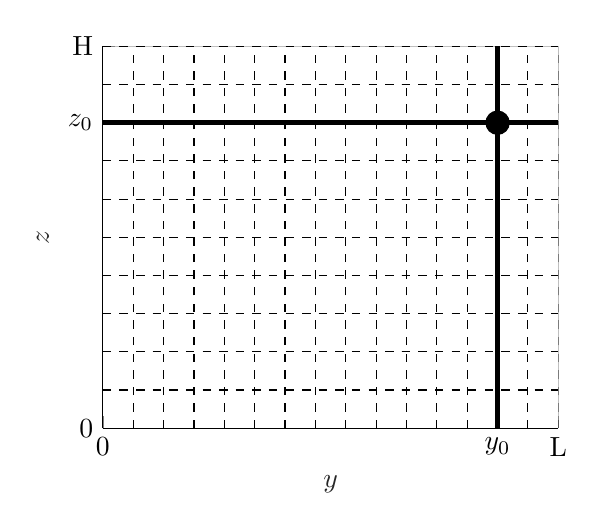
\begin{tikzpicture}

\begin{axis}[%
width=0.477\textwidth,
height=0.4\textwidth,
at={(0\textwidth,0\textwidth)},
scale only axis,
xmin=0,
xmax=15,
xtick={0,13,15},
xticklabels={{0},{$y_0$},{L}},
xlabel style={font=\color{white!15!black}},
xlabel={$y$},
ymin=0,
ymax=5,
ytick={0,4,5},
yticklabels={{0},{$z_0$},{H}},
ylabel style={font=\color{white!15!black}},
ylabel={$z$},
axis background/.style={fill=white},
axis x line*=bottom,
axis y line*=left,
xmajorgrids,
ymajorgrids
]
\addplot [color=black, dashed, forget plot]
  table[row sep=crcr]{%
0	0\\
0	0.0505050505050505\\
0	0.101010101010101\\
0	0.151515151515152\\
0	0.202020202020202\\
0	0.252525252525253\\
0	0.303030303030303\\
0	0.353535353535354\\
0	0.404040404040404\\
0	0.454545454545455\\
0	0.505050505050505\\
0	0.555555555555556\\
0	0.606060606060606\\
0	0.656565656565657\\
0	0.707070707070707\\
0	0.757575757575758\\
0	0.808080808080808\\
0	0.858585858585859\\
0	0.909090909090909\\
0	0.95959595959596\\
0	1.01010101010101\\
0	1.06060606060606\\
0	1.11111111111111\\
0	1.16161616161616\\
0	1.21212121212121\\
0	1.26262626262626\\
0	1.31313131313131\\
0	1.36363636363636\\
0	1.41414141414141\\
0	1.46464646464646\\
0	1.51515151515152\\
0	1.56565656565657\\
0	1.61616161616162\\
0	1.66666666666667\\
0	1.71717171717172\\
0	1.76767676767677\\
0	1.81818181818182\\
0	1.86868686868687\\
0	1.91919191919192\\
0	1.96969696969697\\
0	2.02020202020202\\
0	2.07070707070707\\
0	2.12121212121212\\
0	2.17171717171717\\
0	2.22222222222222\\
0	2.27272727272727\\
0	2.32323232323232\\
0	2.37373737373737\\
0	2.42424242424242\\
0	2.47474747474747\\
0	2.52525252525253\\
0	2.57575757575758\\
0	2.62626262626263\\
0	2.67676767676768\\
0	2.72727272727273\\
0	2.77777777777778\\
0	2.82828282828283\\
0	2.87878787878788\\
0	2.92929292929293\\
0	2.97979797979798\\
0	3.03030303030303\\
0	3.08080808080808\\
0	3.13131313131313\\
0	3.18181818181818\\
0	3.23232323232323\\
0	3.28282828282828\\
0	3.33333333333333\\
0	3.38383838383838\\
0	3.43434343434343\\
0	3.48484848484848\\
0	3.53535353535354\\
0	3.58585858585859\\
0	3.63636363636364\\
0	3.68686868686869\\
0	3.73737373737374\\
0	3.78787878787879\\
0	3.83838383838384\\
0	3.88888888888889\\
0	3.93939393939394\\
0	3.98989898989899\\
0	4.04040404040404\\
0	4.09090909090909\\
0	4.14141414141414\\
0	4.19191919191919\\
0	4.24242424242424\\
0	4.29292929292929\\
0	4.34343434343434\\
0	4.39393939393939\\
0	4.44444444444444\\
0	4.49494949494949\\
0	4.54545454545455\\
0	4.5959595959596\\
0	4.64646464646465\\
0	4.6969696969697\\
0	4.74747474747475\\
0	4.7979797979798\\
0	4.84848484848485\\
0	4.8989898989899\\
0	4.94949494949495\\
0	5\\
};
\addplot [color=black, dashed, forget plot]
  table[row sep=crcr]{%
1	0\\
1	0.0505050505050505\\
1	0.101010101010101\\
1	0.151515151515152\\
1	0.202020202020202\\
1	0.252525252525253\\
1	0.303030303030303\\
1	0.353535353535354\\
1	0.404040404040404\\
1	0.454545454545455\\
1	0.505050505050505\\
1	0.555555555555556\\
1	0.606060606060606\\
1	0.656565656565657\\
1	0.707070707070707\\
1	0.757575757575758\\
1	0.808080808080808\\
1	0.858585858585859\\
1	0.909090909090909\\
1	0.95959595959596\\
1	1.01010101010101\\
1	1.06060606060606\\
1	1.11111111111111\\
1	1.16161616161616\\
1	1.21212121212121\\
1	1.26262626262626\\
1	1.31313131313131\\
1	1.36363636363636\\
1	1.41414141414141\\
1	1.46464646464646\\
1	1.51515151515152\\
1	1.56565656565657\\
1	1.61616161616162\\
1	1.66666666666667\\
1	1.71717171717172\\
1	1.76767676767677\\
1	1.81818181818182\\
1	1.86868686868687\\
1	1.91919191919192\\
1	1.96969696969697\\
1	2.02020202020202\\
1	2.07070707070707\\
1	2.12121212121212\\
1	2.17171717171717\\
1	2.22222222222222\\
1	2.27272727272727\\
1	2.32323232323232\\
1	2.37373737373737\\
1	2.42424242424242\\
1	2.47474747474747\\
1	2.52525252525253\\
1	2.57575757575758\\
1	2.62626262626263\\
1	2.67676767676768\\
1	2.72727272727273\\
1	2.77777777777778\\
1	2.82828282828283\\
1	2.87878787878788\\
1	2.92929292929293\\
1	2.97979797979798\\
1	3.03030303030303\\
1	3.08080808080808\\
1	3.13131313131313\\
1	3.18181818181818\\
1	3.23232323232323\\
1	3.28282828282828\\
1	3.33333333333333\\
1	3.38383838383838\\
1	3.43434343434343\\
1	3.48484848484848\\
1	3.53535353535354\\
1	3.58585858585859\\
1	3.63636363636364\\
1	3.68686868686869\\
1	3.73737373737374\\
1	3.78787878787879\\
1	3.83838383838384\\
1	3.88888888888889\\
1	3.93939393939394\\
1	3.98989898989899\\
1	4.04040404040404\\
1	4.09090909090909\\
1	4.14141414141414\\
1	4.19191919191919\\
1	4.24242424242424\\
1	4.29292929292929\\
1	4.34343434343434\\
1	4.39393939393939\\
1	4.44444444444444\\
1	4.49494949494949\\
1	4.54545454545455\\
1	4.5959595959596\\
1	4.64646464646465\\
1	4.6969696969697\\
1	4.74747474747475\\
1	4.7979797979798\\
1	4.84848484848485\\
1	4.8989898989899\\
1	4.94949494949495\\
1	5\\
};
\addplot [color=black, dashed, forget plot]
  table[row sep=crcr]{%
2	0\\
2	0.0505050505050505\\
2	0.101010101010101\\
2	0.151515151515152\\
2	0.202020202020202\\
2	0.252525252525253\\
2	0.303030303030303\\
2	0.353535353535354\\
2	0.404040404040404\\
2	0.454545454545455\\
2	0.505050505050505\\
2	0.555555555555556\\
2	0.606060606060606\\
2	0.656565656565657\\
2	0.707070707070707\\
2	0.757575757575758\\
2	0.808080808080808\\
2	0.858585858585859\\
2	0.909090909090909\\
2	0.95959595959596\\
2	1.01010101010101\\
2	1.06060606060606\\
2	1.11111111111111\\
2	1.16161616161616\\
2	1.21212121212121\\
2	1.26262626262626\\
2	1.31313131313131\\
2	1.36363636363636\\
2	1.41414141414141\\
2	1.46464646464646\\
2	1.51515151515152\\
2	1.56565656565657\\
2	1.61616161616162\\
2	1.66666666666667\\
2	1.71717171717172\\
2	1.76767676767677\\
2	1.81818181818182\\
2	1.86868686868687\\
2	1.91919191919192\\
2	1.96969696969697\\
2	2.02020202020202\\
2	2.07070707070707\\
2	2.12121212121212\\
2	2.17171717171717\\
2	2.22222222222222\\
2	2.27272727272727\\
2	2.32323232323232\\
2	2.37373737373737\\
2	2.42424242424242\\
2	2.47474747474747\\
2	2.52525252525253\\
2	2.57575757575758\\
2	2.62626262626263\\
2	2.67676767676768\\
2	2.72727272727273\\
2	2.77777777777778\\
2	2.82828282828283\\
2	2.87878787878788\\
2	2.92929292929293\\
2	2.97979797979798\\
2	3.03030303030303\\
2	3.08080808080808\\
2	3.13131313131313\\
2	3.18181818181818\\
2	3.23232323232323\\
2	3.28282828282828\\
2	3.33333333333333\\
2	3.38383838383838\\
2	3.43434343434343\\
2	3.48484848484848\\
2	3.53535353535354\\
2	3.58585858585859\\
2	3.63636363636364\\
2	3.68686868686869\\
2	3.73737373737374\\
2	3.78787878787879\\
2	3.83838383838384\\
2	3.88888888888889\\
2	3.93939393939394\\
2	3.98989898989899\\
2	4.04040404040404\\
2	4.09090909090909\\
2	4.14141414141414\\
2	4.19191919191919\\
2	4.24242424242424\\
2	4.29292929292929\\
2	4.34343434343434\\
2	4.39393939393939\\
2	4.44444444444444\\
2	4.49494949494949\\
2	4.54545454545455\\
2	4.5959595959596\\
2	4.64646464646465\\
2	4.6969696969697\\
2	4.74747474747475\\
2	4.7979797979798\\
2	4.84848484848485\\
2	4.8989898989899\\
2	4.94949494949495\\
2	5\\
};
\addplot [color=black, dashed, forget plot]
  table[row sep=crcr]{%
3	0\\
3	0.0505050505050505\\
3	0.101010101010101\\
3	0.151515151515152\\
3	0.202020202020202\\
3	0.252525252525253\\
3	0.303030303030303\\
3	0.353535353535354\\
3	0.404040404040404\\
3	0.454545454545455\\
3	0.505050505050505\\
3	0.555555555555556\\
3	0.606060606060606\\
3	0.656565656565657\\
3	0.707070707070707\\
3	0.757575757575758\\
3	0.808080808080808\\
3	0.858585858585859\\
3	0.909090909090909\\
3	0.95959595959596\\
3	1.01010101010101\\
3	1.06060606060606\\
3	1.11111111111111\\
3	1.16161616161616\\
3	1.21212121212121\\
3	1.26262626262626\\
3	1.31313131313131\\
3	1.36363636363636\\
3	1.41414141414141\\
3	1.46464646464646\\
3	1.51515151515152\\
3	1.56565656565657\\
3	1.61616161616162\\
3	1.66666666666667\\
3	1.71717171717172\\
3	1.76767676767677\\
3	1.81818181818182\\
3	1.86868686868687\\
3	1.91919191919192\\
3	1.96969696969697\\
3	2.02020202020202\\
3	2.07070707070707\\
3	2.12121212121212\\
3	2.17171717171717\\
3	2.22222222222222\\
3	2.27272727272727\\
3	2.32323232323232\\
3	2.37373737373737\\
3	2.42424242424242\\
3	2.47474747474747\\
3	2.52525252525253\\
3	2.57575757575758\\
3	2.62626262626263\\
3	2.67676767676768\\
3	2.72727272727273\\
3	2.77777777777778\\
3	2.82828282828283\\
3	2.87878787878788\\
3	2.92929292929293\\
3	2.97979797979798\\
3	3.03030303030303\\
3	3.08080808080808\\
3	3.13131313131313\\
3	3.18181818181818\\
3	3.23232323232323\\
3	3.28282828282828\\
3	3.33333333333333\\
3	3.38383838383838\\
3	3.43434343434343\\
3	3.48484848484848\\
3	3.53535353535354\\
3	3.58585858585859\\
3	3.63636363636364\\
3	3.68686868686869\\
3	3.73737373737374\\
3	3.78787878787879\\
3	3.83838383838384\\
3	3.88888888888889\\
3	3.93939393939394\\
3	3.98989898989899\\
3	4.04040404040404\\
3	4.09090909090909\\
3	4.14141414141414\\
3	4.19191919191919\\
3	4.24242424242424\\
3	4.29292929292929\\
3	4.34343434343434\\
3	4.39393939393939\\
3	4.44444444444444\\
3	4.49494949494949\\
3	4.54545454545455\\
3	4.5959595959596\\
3	4.64646464646465\\
3	4.6969696969697\\
3	4.74747474747475\\
3	4.7979797979798\\
3	4.84848484848485\\
3	4.8989898989899\\
3	4.94949494949495\\
3	5\\
};
\addplot [color=black, dashed, forget plot]
  table[row sep=crcr]{%
4	0\\
4	0.0505050505050505\\
4	0.101010101010101\\
4	0.151515151515152\\
4	0.202020202020202\\
4	0.252525252525253\\
4	0.303030303030303\\
4	0.353535353535354\\
4	0.404040404040404\\
4	0.454545454545455\\
4	0.505050505050505\\
4	0.555555555555556\\
4	0.606060606060606\\
4	0.656565656565657\\
4	0.707070707070707\\
4	0.757575757575758\\
4	0.808080808080808\\
4	0.858585858585859\\
4	0.909090909090909\\
4	0.95959595959596\\
4	1.01010101010101\\
4	1.06060606060606\\
4	1.11111111111111\\
4	1.16161616161616\\
4	1.21212121212121\\
4	1.26262626262626\\
4	1.31313131313131\\
4	1.36363636363636\\
4	1.41414141414141\\
4	1.46464646464646\\
4	1.51515151515152\\
4	1.56565656565657\\
4	1.61616161616162\\
4	1.66666666666667\\
4	1.71717171717172\\
4	1.76767676767677\\
4	1.81818181818182\\
4	1.86868686868687\\
4	1.91919191919192\\
4	1.96969696969697\\
4	2.02020202020202\\
4	2.07070707070707\\
4	2.12121212121212\\
4	2.17171717171717\\
4	2.22222222222222\\
4	2.27272727272727\\
4	2.32323232323232\\
4	2.37373737373737\\
4	2.42424242424242\\
4	2.47474747474747\\
4	2.52525252525253\\
4	2.57575757575758\\
4	2.62626262626263\\
4	2.67676767676768\\
4	2.72727272727273\\
4	2.77777777777778\\
4	2.82828282828283\\
4	2.87878787878788\\
4	2.92929292929293\\
4	2.97979797979798\\
4	3.03030303030303\\
4	3.08080808080808\\
4	3.13131313131313\\
4	3.18181818181818\\
4	3.23232323232323\\
4	3.28282828282828\\
4	3.33333333333333\\
4	3.38383838383838\\
4	3.43434343434343\\
4	3.48484848484848\\
4	3.53535353535354\\
4	3.58585858585859\\
4	3.63636363636364\\
4	3.68686868686869\\
4	3.73737373737374\\
4	3.78787878787879\\
4	3.83838383838384\\
4	3.88888888888889\\
4	3.93939393939394\\
4	3.98989898989899\\
4	4.04040404040404\\
4	4.09090909090909\\
4	4.14141414141414\\
4	4.19191919191919\\
4	4.24242424242424\\
4	4.29292929292929\\
4	4.34343434343434\\
4	4.39393939393939\\
4	4.44444444444444\\
4	4.49494949494949\\
4	4.54545454545455\\
4	4.5959595959596\\
4	4.64646464646465\\
4	4.6969696969697\\
4	4.74747474747475\\
4	4.7979797979798\\
4	4.84848484848485\\
4	4.8989898989899\\
4	4.94949494949495\\
4	5\\
};
\addplot [color=black, dashed, forget plot]
  table[row sep=crcr]{%
5	0\\
5	0.0505050505050505\\
5	0.101010101010101\\
5	0.151515151515152\\
5	0.202020202020202\\
5	0.252525252525253\\
5	0.303030303030303\\
5	0.353535353535354\\
5	0.404040404040404\\
5	0.454545454545455\\
5	0.505050505050505\\
5	0.555555555555556\\
5	0.606060606060606\\
5	0.656565656565657\\
5	0.707070707070707\\
5	0.757575757575758\\
5	0.808080808080808\\
5	0.858585858585859\\
5	0.909090909090909\\
5	0.95959595959596\\
5	1.01010101010101\\
5	1.06060606060606\\
5	1.11111111111111\\
5	1.16161616161616\\
5	1.21212121212121\\
5	1.26262626262626\\
5	1.31313131313131\\
5	1.36363636363636\\
5	1.41414141414141\\
5	1.46464646464646\\
5	1.51515151515152\\
5	1.56565656565657\\
5	1.61616161616162\\
5	1.66666666666667\\
5	1.71717171717172\\
5	1.76767676767677\\
5	1.81818181818182\\
5	1.86868686868687\\
5	1.91919191919192\\
5	1.96969696969697\\
5	2.02020202020202\\
5	2.07070707070707\\
5	2.12121212121212\\
5	2.17171717171717\\
5	2.22222222222222\\
5	2.27272727272727\\
5	2.32323232323232\\
5	2.37373737373737\\
5	2.42424242424242\\
5	2.47474747474747\\
5	2.52525252525253\\
5	2.57575757575758\\
5	2.62626262626263\\
5	2.67676767676768\\
5	2.72727272727273\\
5	2.77777777777778\\
5	2.82828282828283\\
5	2.87878787878788\\
5	2.92929292929293\\
5	2.97979797979798\\
5	3.03030303030303\\
5	3.08080808080808\\
5	3.13131313131313\\
5	3.18181818181818\\
5	3.23232323232323\\
5	3.28282828282828\\
5	3.33333333333333\\
5	3.38383838383838\\
5	3.43434343434343\\
5	3.48484848484848\\
5	3.53535353535354\\
5	3.58585858585859\\
5	3.63636363636364\\
5	3.68686868686869\\
5	3.73737373737374\\
5	3.78787878787879\\
5	3.83838383838384\\
5	3.88888888888889\\
5	3.93939393939394\\
5	3.98989898989899\\
5	4.04040404040404\\
5	4.09090909090909\\
5	4.14141414141414\\
5	4.19191919191919\\
5	4.24242424242424\\
5	4.29292929292929\\
5	4.34343434343434\\
5	4.39393939393939\\
5	4.44444444444444\\
5	4.49494949494949\\
5	4.54545454545455\\
5	4.5959595959596\\
5	4.64646464646465\\
5	4.6969696969697\\
5	4.74747474747475\\
5	4.7979797979798\\
5	4.84848484848485\\
5	4.8989898989899\\
5	4.94949494949495\\
5	5\\
};
\addplot [color=black, dashed, forget plot]
  table[row sep=crcr]{%
6	0\\
6	0.0505050505050505\\
6	0.101010101010101\\
6	0.151515151515152\\
6	0.202020202020202\\
6	0.252525252525253\\
6	0.303030303030303\\
6	0.353535353535354\\
6	0.404040404040404\\
6	0.454545454545455\\
6	0.505050505050505\\
6	0.555555555555556\\
6	0.606060606060606\\
6	0.656565656565657\\
6	0.707070707070707\\
6	0.757575757575758\\
6	0.808080808080808\\
6	0.858585858585859\\
6	0.909090909090909\\
6	0.95959595959596\\
6	1.01010101010101\\
6	1.06060606060606\\
6	1.11111111111111\\
6	1.16161616161616\\
6	1.21212121212121\\
6	1.26262626262626\\
6	1.31313131313131\\
6	1.36363636363636\\
6	1.41414141414141\\
6	1.46464646464646\\
6	1.51515151515152\\
6	1.56565656565657\\
6	1.61616161616162\\
6	1.66666666666667\\
6	1.71717171717172\\
6	1.76767676767677\\
6	1.81818181818182\\
6	1.86868686868687\\
6	1.91919191919192\\
6	1.96969696969697\\
6	2.02020202020202\\
6	2.07070707070707\\
6	2.12121212121212\\
6	2.17171717171717\\
6	2.22222222222222\\
6	2.27272727272727\\
6	2.32323232323232\\
6	2.37373737373737\\
6	2.42424242424242\\
6	2.47474747474747\\
6	2.52525252525253\\
6	2.57575757575758\\
6	2.62626262626263\\
6	2.67676767676768\\
6	2.72727272727273\\
6	2.77777777777778\\
6	2.82828282828283\\
6	2.87878787878788\\
6	2.92929292929293\\
6	2.97979797979798\\
6	3.03030303030303\\
6	3.08080808080808\\
6	3.13131313131313\\
6	3.18181818181818\\
6	3.23232323232323\\
6	3.28282828282828\\
6	3.33333333333333\\
6	3.38383838383838\\
6	3.43434343434343\\
6	3.48484848484848\\
6	3.53535353535354\\
6	3.58585858585859\\
6	3.63636363636364\\
6	3.68686868686869\\
6	3.73737373737374\\
6	3.78787878787879\\
6	3.83838383838384\\
6	3.88888888888889\\
6	3.93939393939394\\
6	3.98989898989899\\
6	4.04040404040404\\
6	4.09090909090909\\
6	4.14141414141414\\
6	4.19191919191919\\
6	4.24242424242424\\
6	4.29292929292929\\
6	4.34343434343434\\
6	4.39393939393939\\
6	4.44444444444444\\
6	4.49494949494949\\
6	4.54545454545455\\
6	4.5959595959596\\
6	4.64646464646465\\
6	4.6969696969697\\
6	4.74747474747475\\
6	4.7979797979798\\
6	4.84848484848485\\
6	4.8989898989899\\
6	4.94949494949495\\
6	5\\
};
\addplot [color=black, dashed, forget plot]
  table[row sep=crcr]{%
7	0\\
7	0.0505050505050505\\
7	0.101010101010101\\
7	0.151515151515152\\
7	0.202020202020202\\
7	0.252525252525253\\
7	0.303030303030303\\
7	0.353535353535354\\
7	0.404040404040404\\
7	0.454545454545455\\
7	0.505050505050505\\
7	0.555555555555556\\
7	0.606060606060606\\
7	0.656565656565657\\
7	0.707070707070707\\
7	0.757575757575758\\
7	0.808080808080808\\
7	0.858585858585859\\
7	0.909090909090909\\
7	0.95959595959596\\
7	1.01010101010101\\
7	1.06060606060606\\
7	1.11111111111111\\
7	1.16161616161616\\
7	1.21212121212121\\
7	1.26262626262626\\
7	1.31313131313131\\
7	1.36363636363636\\
7	1.41414141414141\\
7	1.46464646464646\\
7	1.51515151515152\\
7	1.56565656565657\\
7	1.61616161616162\\
7	1.66666666666667\\
7	1.71717171717172\\
7	1.76767676767677\\
7	1.81818181818182\\
7	1.86868686868687\\
7	1.91919191919192\\
7	1.96969696969697\\
7	2.02020202020202\\
7	2.07070707070707\\
7	2.12121212121212\\
7	2.17171717171717\\
7	2.22222222222222\\
7	2.27272727272727\\
7	2.32323232323232\\
7	2.37373737373737\\
7	2.42424242424242\\
7	2.47474747474747\\
7	2.52525252525253\\
7	2.57575757575758\\
7	2.62626262626263\\
7	2.67676767676768\\
7	2.72727272727273\\
7	2.77777777777778\\
7	2.82828282828283\\
7	2.87878787878788\\
7	2.92929292929293\\
7	2.97979797979798\\
7	3.03030303030303\\
7	3.08080808080808\\
7	3.13131313131313\\
7	3.18181818181818\\
7	3.23232323232323\\
7	3.28282828282828\\
7	3.33333333333333\\
7	3.38383838383838\\
7	3.43434343434343\\
7	3.48484848484848\\
7	3.53535353535354\\
7	3.58585858585859\\
7	3.63636363636364\\
7	3.68686868686869\\
7	3.73737373737374\\
7	3.78787878787879\\
7	3.83838383838384\\
7	3.88888888888889\\
7	3.93939393939394\\
7	3.98989898989899\\
7	4.04040404040404\\
7	4.09090909090909\\
7	4.14141414141414\\
7	4.19191919191919\\
7	4.24242424242424\\
7	4.29292929292929\\
7	4.34343434343434\\
7	4.39393939393939\\
7	4.44444444444444\\
7	4.49494949494949\\
7	4.54545454545455\\
7	4.5959595959596\\
7	4.64646464646465\\
7	4.6969696969697\\
7	4.74747474747475\\
7	4.7979797979798\\
7	4.84848484848485\\
7	4.8989898989899\\
7	4.94949494949495\\
7	5\\
};
\addplot [color=black, dashed, forget plot]
  table[row sep=crcr]{%
8	0\\
8	0.0505050505050505\\
8	0.101010101010101\\
8	0.151515151515152\\
8	0.202020202020202\\
8	0.252525252525253\\
8	0.303030303030303\\
8	0.353535353535354\\
8	0.404040404040404\\
8	0.454545454545455\\
8	0.505050505050505\\
8	0.555555555555556\\
8	0.606060606060606\\
8	0.656565656565657\\
8	0.707070707070707\\
8	0.757575757575758\\
8	0.808080808080808\\
8	0.858585858585859\\
8	0.909090909090909\\
8	0.95959595959596\\
8	1.01010101010101\\
8	1.06060606060606\\
8	1.11111111111111\\
8	1.16161616161616\\
8	1.21212121212121\\
8	1.26262626262626\\
8	1.31313131313131\\
8	1.36363636363636\\
8	1.41414141414141\\
8	1.46464646464646\\
8	1.51515151515152\\
8	1.56565656565657\\
8	1.61616161616162\\
8	1.66666666666667\\
8	1.71717171717172\\
8	1.76767676767677\\
8	1.81818181818182\\
8	1.86868686868687\\
8	1.91919191919192\\
8	1.96969696969697\\
8	2.02020202020202\\
8	2.07070707070707\\
8	2.12121212121212\\
8	2.17171717171717\\
8	2.22222222222222\\
8	2.27272727272727\\
8	2.32323232323232\\
8	2.37373737373737\\
8	2.42424242424242\\
8	2.47474747474747\\
8	2.52525252525253\\
8	2.57575757575758\\
8	2.62626262626263\\
8	2.67676767676768\\
8	2.72727272727273\\
8	2.77777777777778\\
8	2.82828282828283\\
8	2.87878787878788\\
8	2.92929292929293\\
8	2.97979797979798\\
8	3.03030303030303\\
8	3.08080808080808\\
8	3.13131313131313\\
8	3.18181818181818\\
8	3.23232323232323\\
8	3.28282828282828\\
8	3.33333333333333\\
8	3.38383838383838\\
8	3.43434343434343\\
8	3.48484848484848\\
8	3.53535353535354\\
8	3.58585858585859\\
8	3.63636363636364\\
8	3.68686868686869\\
8	3.73737373737374\\
8	3.78787878787879\\
8	3.83838383838384\\
8	3.88888888888889\\
8	3.93939393939394\\
8	3.98989898989899\\
8	4.04040404040404\\
8	4.09090909090909\\
8	4.14141414141414\\
8	4.19191919191919\\
8	4.24242424242424\\
8	4.29292929292929\\
8	4.34343434343434\\
8	4.39393939393939\\
8	4.44444444444444\\
8	4.49494949494949\\
8	4.54545454545455\\
8	4.5959595959596\\
8	4.64646464646465\\
8	4.6969696969697\\
8	4.74747474747475\\
8	4.7979797979798\\
8	4.84848484848485\\
8	4.8989898989899\\
8	4.94949494949495\\
8	5\\
};
\addplot [color=black, dashed, forget plot]
  table[row sep=crcr]{%
9	0\\
9	0.0505050505050505\\
9	0.101010101010101\\
9	0.151515151515152\\
9	0.202020202020202\\
9	0.252525252525253\\
9	0.303030303030303\\
9	0.353535353535354\\
9	0.404040404040404\\
9	0.454545454545455\\
9	0.505050505050505\\
9	0.555555555555556\\
9	0.606060606060606\\
9	0.656565656565657\\
9	0.707070707070707\\
9	0.757575757575758\\
9	0.808080808080808\\
9	0.858585858585859\\
9	0.909090909090909\\
9	0.95959595959596\\
9	1.01010101010101\\
9	1.06060606060606\\
9	1.11111111111111\\
9	1.16161616161616\\
9	1.21212121212121\\
9	1.26262626262626\\
9	1.31313131313131\\
9	1.36363636363636\\
9	1.41414141414141\\
9	1.46464646464646\\
9	1.51515151515152\\
9	1.56565656565657\\
9	1.61616161616162\\
9	1.66666666666667\\
9	1.71717171717172\\
9	1.76767676767677\\
9	1.81818181818182\\
9	1.86868686868687\\
9	1.91919191919192\\
9	1.96969696969697\\
9	2.02020202020202\\
9	2.07070707070707\\
9	2.12121212121212\\
9	2.17171717171717\\
9	2.22222222222222\\
9	2.27272727272727\\
9	2.32323232323232\\
9	2.37373737373737\\
9	2.42424242424242\\
9	2.47474747474747\\
9	2.52525252525253\\
9	2.57575757575758\\
9	2.62626262626263\\
9	2.67676767676768\\
9	2.72727272727273\\
9	2.77777777777778\\
9	2.82828282828283\\
9	2.87878787878788\\
9	2.92929292929293\\
9	2.97979797979798\\
9	3.03030303030303\\
9	3.08080808080808\\
9	3.13131313131313\\
9	3.18181818181818\\
9	3.23232323232323\\
9	3.28282828282828\\
9	3.33333333333333\\
9	3.38383838383838\\
9	3.43434343434343\\
9	3.48484848484848\\
9	3.53535353535354\\
9	3.58585858585859\\
9	3.63636363636364\\
9	3.68686868686869\\
9	3.73737373737374\\
9	3.78787878787879\\
9	3.83838383838384\\
9	3.88888888888889\\
9	3.93939393939394\\
9	3.98989898989899\\
9	4.04040404040404\\
9	4.09090909090909\\
9	4.14141414141414\\
9	4.19191919191919\\
9	4.24242424242424\\
9	4.29292929292929\\
9	4.34343434343434\\
9	4.39393939393939\\
9	4.44444444444444\\
9	4.49494949494949\\
9	4.54545454545455\\
9	4.5959595959596\\
9	4.64646464646465\\
9	4.6969696969697\\
9	4.74747474747475\\
9	4.7979797979798\\
9	4.84848484848485\\
9	4.8989898989899\\
9	4.94949494949495\\
9	5\\
};
\addplot [color=black, dashed, forget plot]
  table[row sep=crcr]{%
10	0\\
10	0.0505050505050505\\
10	0.101010101010101\\
10	0.151515151515152\\
10	0.202020202020202\\
10	0.252525252525253\\
10	0.303030303030303\\
10	0.353535353535354\\
10	0.404040404040404\\
10	0.454545454545455\\
10	0.505050505050505\\
10	0.555555555555556\\
10	0.606060606060606\\
10	0.656565656565657\\
10	0.707070707070707\\
10	0.757575757575758\\
10	0.808080808080808\\
10	0.858585858585859\\
10	0.909090909090909\\
10	0.95959595959596\\
10	1.01010101010101\\
10	1.06060606060606\\
10	1.11111111111111\\
10	1.16161616161616\\
10	1.21212121212121\\
10	1.26262626262626\\
10	1.31313131313131\\
10	1.36363636363636\\
10	1.41414141414141\\
10	1.46464646464646\\
10	1.51515151515152\\
10	1.56565656565657\\
10	1.61616161616162\\
10	1.66666666666667\\
10	1.71717171717172\\
10	1.76767676767677\\
10	1.81818181818182\\
10	1.86868686868687\\
10	1.91919191919192\\
10	1.96969696969697\\
10	2.02020202020202\\
10	2.07070707070707\\
10	2.12121212121212\\
10	2.17171717171717\\
10	2.22222222222222\\
10	2.27272727272727\\
10	2.32323232323232\\
10	2.37373737373737\\
10	2.42424242424242\\
10	2.47474747474747\\
10	2.52525252525253\\
10	2.57575757575758\\
10	2.62626262626263\\
10	2.67676767676768\\
10	2.72727272727273\\
10	2.77777777777778\\
10	2.82828282828283\\
10	2.87878787878788\\
10	2.92929292929293\\
10	2.97979797979798\\
10	3.03030303030303\\
10	3.08080808080808\\
10	3.13131313131313\\
10	3.18181818181818\\
10	3.23232323232323\\
10	3.28282828282828\\
10	3.33333333333333\\
10	3.38383838383838\\
10	3.43434343434343\\
10	3.48484848484848\\
10	3.53535353535354\\
10	3.58585858585859\\
10	3.63636363636364\\
10	3.68686868686869\\
10	3.73737373737374\\
10	3.78787878787879\\
10	3.83838383838384\\
10	3.88888888888889\\
10	3.93939393939394\\
10	3.98989898989899\\
10	4.04040404040404\\
10	4.09090909090909\\
10	4.14141414141414\\
10	4.19191919191919\\
10	4.24242424242424\\
10	4.29292929292929\\
10	4.34343434343434\\
10	4.39393939393939\\
10	4.44444444444444\\
10	4.49494949494949\\
10	4.54545454545455\\
10	4.5959595959596\\
10	4.64646464646465\\
10	4.6969696969697\\
10	4.74747474747475\\
10	4.7979797979798\\
10	4.84848484848485\\
10	4.8989898989899\\
10	4.94949494949495\\
10	5\\
};
\addplot [color=black, dashed, forget plot]
  table[row sep=crcr]{%
11	0\\
11	0.0505050505050505\\
11	0.101010101010101\\
11	0.151515151515152\\
11	0.202020202020202\\
11	0.252525252525253\\
11	0.303030303030303\\
11	0.353535353535354\\
11	0.404040404040404\\
11	0.454545454545455\\
11	0.505050505050505\\
11	0.555555555555556\\
11	0.606060606060606\\
11	0.656565656565657\\
11	0.707070707070707\\
11	0.757575757575758\\
11	0.808080808080808\\
11	0.858585858585859\\
11	0.909090909090909\\
11	0.95959595959596\\
11	1.01010101010101\\
11	1.06060606060606\\
11	1.11111111111111\\
11	1.16161616161616\\
11	1.21212121212121\\
11	1.26262626262626\\
11	1.31313131313131\\
11	1.36363636363636\\
11	1.41414141414141\\
11	1.46464646464646\\
11	1.51515151515152\\
11	1.56565656565657\\
11	1.61616161616162\\
11	1.66666666666667\\
11	1.71717171717172\\
11	1.76767676767677\\
11	1.81818181818182\\
11	1.86868686868687\\
11	1.91919191919192\\
11	1.96969696969697\\
11	2.02020202020202\\
11	2.07070707070707\\
11	2.12121212121212\\
11	2.17171717171717\\
11	2.22222222222222\\
11	2.27272727272727\\
11	2.32323232323232\\
11	2.37373737373737\\
11	2.42424242424242\\
11	2.47474747474747\\
11	2.52525252525253\\
11	2.57575757575758\\
11	2.62626262626263\\
11	2.67676767676768\\
11	2.72727272727273\\
11	2.77777777777778\\
11	2.82828282828283\\
11	2.87878787878788\\
11	2.92929292929293\\
11	2.97979797979798\\
11	3.03030303030303\\
11	3.08080808080808\\
11	3.13131313131313\\
11	3.18181818181818\\
11	3.23232323232323\\
11	3.28282828282828\\
11	3.33333333333333\\
11	3.38383838383838\\
11	3.43434343434343\\
11	3.48484848484848\\
11	3.53535353535354\\
11	3.58585858585859\\
11	3.63636363636364\\
11	3.68686868686869\\
11	3.73737373737374\\
11	3.78787878787879\\
11	3.83838383838384\\
11	3.88888888888889\\
11	3.93939393939394\\
11	3.98989898989899\\
11	4.04040404040404\\
11	4.09090909090909\\
11	4.14141414141414\\
11	4.19191919191919\\
11	4.24242424242424\\
11	4.29292929292929\\
11	4.34343434343434\\
11	4.39393939393939\\
11	4.44444444444444\\
11	4.49494949494949\\
11	4.54545454545455\\
11	4.5959595959596\\
11	4.64646464646465\\
11	4.6969696969697\\
11	4.74747474747475\\
11	4.7979797979798\\
11	4.84848484848485\\
11	4.8989898989899\\
11	4.94949494949495\\
11	5\\
};
\addplot [color=black, dashed, forget plot]
  table[row sep=crcr]{%
12	0\\
12	0.0505050505050505\\
12	0.101010101010101\\
12	0.151515151515152\\
12	0.202020202020202\\
12	0.252525252525253\\
12	0.303030303030303\\
12	0.353535353535354\\
12	0.404040404040404\\
12	0.454545454545455\\
12	0.505050505050505\\
12	0.555555555555556\\
12	0.606060606060606\\
12	0.656565656565657\\
12	0.707070707070707\\
12	0.757575757575758\\
12	0.808080808080808\\
12	0.858585858585859\\
12	0.909090909090909\\
12	0.95959595959596\\
12	1.01010101010101\\
12	1.06060606060606\\
12	1.11111111111111\\
12	1.16161616161616\\
12	1.21212121212121\\
12	1.26262626262626\\
12	1.31313131313131\\
12	1.36363636363636\\
12	1.41414141414141\\
12	1.46464646464646\\
12	1.51515151515152\\
12	1.56565656565657\\
12	1.61616161616162\\
12	1.66666666666667\\
12	1.71717171717172\\
12	1.76767676767677\\
12	1.81818181818182\\
12	1.86868686868687\\
12	1.91919191919192\\
12	1.96969696969697\\
12	2.02020202020202\\
12	2.07070707070707\\
12	2.12121212121212\\
12	2.17171717171717\\
12	2.22222222222222\\
12	2.27272727272727\\
12	2.32323232323232\\
12	2.37373737373737\\
12	2.42424242424242\\
12	2.47474747474747\\
12	2.52525252525253\\
12	2.57575757575758\\
12	2.62626262626263\\
12	2.67676767676768\\
12	2.72727272727273\\
12	2.77777777777778\\
12	2.82828282828283\\
12	2.87878787878788\\
12	2.92929292929293\\
12	2.97979797979798\\
12	3.03030303030303\\
12	3.08080808080808\\
12	3.13131313131313\\
12	3.18181818181818\\
12	3.23232323232323\\
12	3.28282828282828\\
12	3.33333333333333\\
12	3.38383838383838\\
12	3.43434343434343\\
12	3.48484848484848\\
12	3.53535353535354\\
12	3.58585858585859\\
12	3.63636363636364\\
12	3.68686868686869\\
12	3.73737373737374\\
12	3.78787878787879\\
12	3.83838383838384\\
12	3.88888888888889\\
12	3.93939393939394\\
12	3.98989898989899\\
12	4.04040404040404\\
12	4.09090909090909\\
12	4.14141414141414\\
12	4.19191919191919\\
12	4.24242424242424\\
12	4.29292929292929\\
12	4.34343434343434\\
12	4.39393939393939\\
12	4.44444444444444\\
12	4.49494949494949\\
12	4.54545454545455\\
12	4.5959595959596\\
12	4.64646464646465\\
12	4.6969696969697\\
12	4.74747474747475\\
12	4.7979797979798\\
12	4.84848484848485\\
12	4.8989898989899\\
12	4.94949494949495\\
12	5\\
};
\addplot [color=black, dashed, forget plot]
  table[row sep=crcr]{%
13	0\\
13	0.0505050505050505\\
13	0.101010101010101\\
13	0.151515151515152\\
13	0.202020202020202\\
13	0.252525252525253\\
13	0.303030303030303\\
13	0.353535353535354\\
13	0.404040404040404\\
13	0.454545454545455\\
13	0.505050505050505\\
13	0.555555555555556\\
13	0.606060606060606\\
13	0.656565656565657\\
13	0.707070707070707\\
13	0.757575757575758\\
13	0.808080808080808\\
13	0.858585858585859\\
13	0.909090909090909\\
13	0.95959595959596\\
13	1.01010101010101\\
13	1.06060606060606\\
13	1.11111111111111\\
13	1.16161616161616\\
13	1.21212121212121\\
13	1.26262626262626\\
13	1.31313131313131\\
13	1.36363636363636\\
13	1.41414141414141\\
13	1.46464646464646\\
13	1.51515151515152\\
13	1.56565656565657\\
13	1.61616161616162\\
13	1.66666666666667\\
13	1.71717171717172\\
13	1.76767676767677\\
13	1.81818181818182\\
13	1.86868686868687\\
13	1.91919191919192\\
13	1.96969696969697\\
13	2.02020202020202\\
13	2.07070707070707\\
13	2.12121212121212\\
13	2.17171717171717\\
13	2.22222222222222\\
13	2.27272727272727\\
13	2.32323232323232\\
13	2.37373737373737\\
13	2.42424242424242\\
13	2.47474747474747\\
13	2.52525252525253\\
13	2.57575757575758\\
13	2.62626262626263\\
13	2.67676767676768\\
13	2.72727272727273\\
13	2.77777777777778\\
13	2.82828282828283\\
13	2.87878787878788\\
13	2.92929292929293\\
13	2.97979797979798\\
13	3.03030303030303\\
13	3.08080808080808\\
13	3.13131313131313\\
13	3.18181818181818\\
13	3.23232323232323\\
13	3.28282828282828\\
13	3.33333333333333\\
13	3.38383838383838\\
13	3.43434343434343\\
13	3.48484848484848\\
13	3.53535353535354\\
13	3.58585858585859\\
13	3.63636363636364\\
13	3.68686868686869\\
13	3.73737373737374\\
13	3.78787878787879\\
13	3.83838383838384\\
13	3.88888888888889\\
13	3.93939393939394\\
13	3.98989898989899\\
13	4.04040404040404\\
13	4.09090909090909\\
13	4.14141414141414\\
13	4.19191919191919\\
13	4.24242424242424\\
13	4.29292929292929\\
13	4.34343434343434\\
13	4.39393939393939\\
13	4.44444444444444\\
13	4.49494949494949\\
13	4.54545454545455\\
13	4.5959595959596\\
13	4.64646464646465\\
13	4.6969696969697\\
13	4.74747474747475\\
13	4.7979797979798\\
13	4.84848484848485\\
13	4.8989898989899\\
13	4.94949494949495\\
13	5\\
};
\addplot [color=black, dashed, forget plot]
  table[row sep=crcr]{%
14	0\\
14	0.0505050505050505\\
14	0.101010101010101\\
14	0.151515151515152\\
14	0.202020202020202\\
14	0.252525252525253\\
14	0.303030303030303\\
14	0.353535353535354\\
14	0.404040404040404\\
14	0.454545454545455\\
14	0.505050505050505\\
14	0.555555555555556\\
14	0.606060606060606\\
14	0.656565656565657\\
14	0.707070707070707\\
14	0.757575757575758\\
14	0.808080808080808\\
14	0.858585858585859\\
14	0.909090909090909\\
14	0.95959595959596\\
14	1.01010101010101\\
14	1.06060606060606\\
14	1.11111111111111\\
14	1.16161616161616\\
14	1.21212121212121\\
14	1.26262626262626\\
14	1.31313131313131\\
14	1.36363636363636\\
14	1.41414141414141\\
14	1.46464646464646\\
14	1.51515151515152\\
14	1.56565656565657\\
14	1.61616161616162\\
14	1.66666666666667\\
14	1.71717171717172\\
14	1.76767676767677\\
14	1.81818181818182\\
14	1.86868686868687\\
14	1.91919191919192\\
14	1.96969696969697\\
14	2.02020202020202\\
14	2.07070707070707\\
14	2.12121212121212\\
14	2.17171717171717\\
14	2.22222222222222\\
14	2.27272727272727\\
14	2.32323232323232\\
14	2.37373737373737\\
14	2.42424242424242\\
14	2.47474747474747\\
14	2.52525252525253\\
14	2.57575757575758\\
14	2.62626262626263\\
14	2.67676767676768\\
14	2.72727272727273\\
14	2.77777777777778\\
14	2.82828282828283\\
14	2.87878787878788\\
14	2.92929292929293\\
14	2.97979797979798\\
14	3.03030303030303\\
14	3.08080808080808\\
14	3.13131313131313\\
14	3.18181818181818\\
14	3.23232323232323\\
14	3.28282828282828\\
14	3.33333333333333\\
14	3.38383838383838\\
14	3.43434343434343\\
14	3.48484848484848\\
14	3.53535353535354\\
14	3.58585858585859\\
14	3.63636363636364\\
14	3.68686868686869\\
14	3.73737373737374\\
14	3.78787878787879\\
14	3.83838383838384\\
14	3.88888888888889\\
14	3.93939393939394\\
14	3.98989898989899\\
14	4.04040404040404\\
14	4.09090909090909\\
14	4.14141414141414\\
14	4.19191919191919\\
14	4.24242424242424\\
14	4.29292929292929\\
14	4.34343434343434\\
14	4.39393939393939\\
14	4.44444444444444\\
14	4.49494949494949\\
14	4.54545454545455\\
14	4.5959595959596\\
14	4.64646464646465\\
14	4.6969696969697\\
14	4.74747474747475\\
14	4.7979797979798\\
14	4.84848484848485\\
14	4.8989898989899\\
14	4.94949494949495\\
14	5\\
};
\addplot [color=black, dashed, forget plot]
  table[row sep=crcr]{%
15	0\\
15	0.0505050505050505\\
15	0.101010101010101\\
15	0.151515151515152\\
15	0.202020202020202\\
15	0.252525252525253\\
15	0.303030303030303\\
15	0.353535353535354\\
15	0.404040404040404\\
15	0.454545454545455\\
15	0.505050505050505\\
15	0.555555555555556\\
15	0.606060606060606\\
15	0.656565656565657\\
15	0.707070707070707\\
15	0.757575757575758\\
15	0.808080808080808\\
15	0.858585858585859\\
15	0.909090909090909\\
15	0.95959595959596\\
15	1.01010101010101\\
15	1.06060606060606\\
15	1.11111111111111\\
15	1.16161616161616\\
15	1.21212121212121\\
15	1.26262626262626\\
15	1.31313131313131\\
15	1.36363636363636\\
15	1.41414141414141\\
15	1.46464646464646\\
15	1.51515151515152\\
15	1.56565656565657\\
15	1.61616161616162\\
15	1.66666666666667\\
15	1.71717171717172\\
15	1.76767676767677\\
15	1.81818181818182\\
15	1.86868686868687\\
15	1.91919191919192\\
15	1.96969696969697\\
15	2.02020202020202\\
15	2.07070707070707\\
15	2.12121212121212\\
15	2.17171717171717\\
15	2.22222222222222\\
15	2.27272727272727\\
15	2.32323232323232\\
15	2.37373737373737\\
15	2.42424242424242\\
15	2.47474747474747\\
15	2.52525252525253\\
15	2.57575757575758\\
15	2.62626262626263\\
15	2.67676767676768\\
15	2.72727272727273\\
15	2.77777777777778\\
15	2.82828282828283\\
15	2.87878787878788\\
15	2.92929292929293\\
15	2.97979797979798\\
15	3.03030303030303\\
15	3.08080808080808\\
15	3.13131313131313\\
15	3.18181818181818\\
15	3.23232323232323\\
15	3.28282828282828\\
15	3.33333333333333\\
15	3.38383838383838\\
15	3.43434343434343\\
15	3.48484848484848\\
15	3.53535353535354\\
15	3.58585858585859\\
15	3.63636363636364\\
15	3.68686868686869\\
15	3.73737373737374\\
15	3.78787878787879\\
15	3.83838383838384\\
15	3.88888888888889\\
15	3.93939393939394\\
15	3.98989898989899\\
15	4.04040404040404\\
15	4.09090909090909\\
15	4.14141414141414\\
15	4.19191919191919\\
15	4.24242424242424\\
15	4.29292929292929\\
15	4.34343434343434\\
15	4.39393939393939\\
15	4.44444444444444\\
15	4.49494949494949\\
15	4.54545454545455\\
15	4.5959595959596\\
15	4.64646464646465\\
15	4.6969696969697\\
15	4.74747474747475\\
15	4.7979797979798\\
15	4.84848484848485\\
15	4.8989898989899\\
15	4.94949494949495\\
15	5\\
};
\addplot [color=black, dashed, forget plot]
  table[row sep=crcr]{%
0	0\\
0.151515151515152	0\\
0.303030303030303	0\\
0.454545454545455	0\\
0.606060606060606	0\\
0.757575757575758	0\\
0.909090909090909	0\\
1.06060606060606	0\\
1.21212121212121	0\\
1.36363636363636	0\\
1.51515151515152	0\\
1.66666666666667	0\\
1.81818181818182	0\\
1.96969696969697	0\\
2.12121212121212	0\\
2.27272727272727	0\\
2.42424242424242	0\\
2.57575757575758	0\\
2.72727272727273	0\\
2.87878787878788	0\\
3.03030303030303	0\\
3.18181818181818	0\\
3.33333333333333	0\\
3.48484848484848	0\\
3.63636363636364	0\\
3.78787878787879	0\\
3.93939393939394	0\\
4.09090909090909	0\\
4.24242424242424	0\\
4.39393939393939	0\\
4.54545454545455	0\\
4.6969696969697	0\\
4.84848484848485	0\\
5	0\\
5.15151515151515	0\\
5.3030303030303	0\\
5.45454545454545	0\\
5.60606060606061	0\\
5.75757575757576	0\\
5.90909090909091	0\\
6.06060606060606	0\\
6.21212121212121	0\\
6.36363636363636	0\\
6.51515151515152	0\\
6.66666666666667	0\\
6.81818181818182	0\\
6.96969696969697	0\\
7.12121212121212	0\\
7.27272727272727	0\\
7.42424242424242	0\\
7.57575757575758	0\\
7.72727272727273	0\\
7.87878787878788	0\\
8.03030303030303	0\\
8.18181818181818	0\\
8.33333333333333	0\\
8.48484848484848	0\\
8.63636363636364	0\\
8.78787878787879	0\\
8.93939393939394	0\\
9.09090909090909	0\\
9.24242424242424	0\\
9.39393939393939	0\\
9.54545454545454	0\\
9.6969696969697	0\\
9.84848484848485	0\\
10	0\\
10.1515151515152	0\\
10.3030303030303	0\\
10.4545454545455	0\\
10.6060606060606	0\\
10.7575757575758	0\\
10.9090909090909	0\\
11.0606060606061	0\\
11.2121212121212	0\\
11.3636363636364	0\\
11.5151515151515	0\\
11.6666666666667	0\\
11.8181818181818	0\\
11.969696969697	0\\
12.1212121212121	0\\
12.2727272727273	0\\
12.4242424242424	0\\
12.5757575757576	0\\
12.7272727272727	0\\
12.8787878787879	0\\
13.030303030303	0\\
13.1818181818182	0\\
13.3333333333333	0\\
13.4848484848485	0\\
13.6363636363636	0\\
13.7878787878788	0\\
13.9393939393939	0\\
14.0909090909091	0\\
14.2424242424242	0\\
14.3939393939394	0\\
14.5454545454545	0\\
14.6969696969697	0\\
14.8484848484848	0\\
15	0\\
};
\addplot [color=black, dashed, forget plot]
  table[row sep=crcr]{%
0	0.5\\
0.151515151515152	0.5\\
0.303030303030303	0.5\\
0.454545454545455	0.5\\
0.606060606060606	0.5\\
0.757575757575758	0.5\\
0.909090909090909	0.5\\
1.06060606060606	0.5\\
1.21212121212121	0.5\\
1.36363636363636	0.5\\
1.51515151515152	0.5\\
1.66666666666667	0.5\\
1.81818181818182	0.5\\
1.96969696969697	0.5\\
2.12121212121212	0.5\\
2.27272727272727	0.5\\
2.42424242424242	0.5\\
2.57575757575758	0.5\\
2.72727272727273	0.5\\
2.87878787878788	0.5\\
3.03030303030303	0.5\\
3.18181818181818	0.5\\
3.33333333333333	0.5\\
3.48484848484848	0.5\\
3.63636363636364	0.5\\
3.78787878787879	0.5\\
3.93939393939394	0.5\\
4.09090909090909	0.5\\
4.24242424242424	0.5\\
4.39393939393939	0.5\\
4.54545454545455	0.5\\
4.6969696969697	0.5\\
4.84848484848485	0.5\\
5	0.5\\
5.15151515151515	0.5\\
5.3030303030303	0.5\\
5.45454545454545	0.5\\
5.60606060606061	0.5\\
5.75757575757576	0.5\\
5.90909090909091	0.5\\
6.06060606060606	0.5\\
6.21212121212121	0.5\\
6.36363636363636	0.5\\
6.51515151515152	0.5\\
6.66666666666667	0.5\\
6.81818181818182	0.5\\
6.96969696969697	0.5\\
7.12121212121212	0.5\\
7.27272727272727	0.5\\
7.42424242424242	0.5\\
7.57575757575758	0.5\\
7.72727272727273	0.5\\
7.87878787878788	0.5\\
8.03030303030303	0.5\\
8.18181818181818	0.5\\
8.33333333333333	0.5\\
8.48484848484848	0.5\\
8.63636363636364	0.5\\
8.78787878787879	0.5\\
8.93939393939394	0.5\\
9.09090909090909	0.5\\
9.24242424242424	0.5\\
9.39393939393939	0.5\\
9.54545454545454	0.5\\
9.6969696969697	0.5\\
9.84848484848485	0.5\\
10	0.5\\
10.1515151515152	0.5\\
10.3030303030303	0.5\\
10.4545454545455	0.5\\
10.6060606060606	0.5\\
10.7575757575758	0.5\\
10.9090909090909	0.5\\
11.0606060606061	0.5\\
11.2121212121212	0.5\\
11.3636363636364	0.5\\
11.5151515151515	0.5\\
11.6666666666667	0.5\\
11.8181818181818	0.5\\
11.969696969697	0.5\\
12.1212121212121	0.5\\
12.2727272727273	0.5\\
12.4242424242424	0.5\\
12.5757575757576	0.5\\
12.7272727272727	0.5\\
12.8787878787879	0.5\\
13.030303030303	0.5\\
13.1818181818182	0.5\\
13.3333333333333	0.5\\
13.4848484848485	0.5\\
13.6363636363636	0.5\\
13.7878787878788	0.5\\
13.9393939393939	0.5\\
14.0909090909091	0.5\\
14.2424242424242	0.5\\
14.3939393939394	0.5\\
14.5454545454545	0.5\\
14.6969696969697	0.5\\
14.8484848484848	0.5\\
15	0.5\\
};
\addplot [color=black, dashed, forget plot]
  table[row sep=crcr]{%
0	1\\
0.151515151515152	1\\
0.303030303030303	1\\
0.454545454545455	1\\
0.606060606060606	1\\
0.757575757575758	1\\
0.909090909090909	1\\
1.06060606060606	1\\
1.21212121212121	1\\
1.36363636363636	1\\
1.51515151515152	1\\
1.66666666666667	1\\
1.81818181818182	1\\
1.96969696969697	1\\
2.12121212121212	1\\
2.27272727272727	1\\
2.42424242424242	1\\
2.57575757575758	1\\
2.72727272727273	1\\
2.87878787878788	1\\
3.03030303030303	1\\
3.18181818181818	1\\
3.33333333333333	1\\
3.48484848484848	1\\
3.63636363636364	1\\
3.78787878787879	1\\
3.93939393939394	1\\
4.09090909090909	1\\
4.24242424242424	1\\
4.39393939393939	1\\
4.54545454545455	1\\
4.6969696969697	1\\
4.84848484848485	1\\
5	1\\
5.15151515151515	1\\
5.3030303030303	1\\
5.45454545454545	1\\
5.60606060606061	1\\
5.75757575757576	1\\
5.90909090909091	1\\
6.06060606060606	1\\
6.21212121212121	1\\
6.36363636363636	1\\
6.51515151515152	1\\
6.66666666666667	1\\
6.81818181818182	1\\
6.96969696969697	1\\
7.12121212121212	1\\
7.27272727272727	1\\
7.42424242424242	1\\
7.57575757575758	1\\
7.72727272727273	1\\
7.87878787878788	1\\
8.03030303030303	1\\
8.18181818181818	1\\
8.33333333333333	1\\
8.48484848484848	1\\
8.63636363636364	1\\
8.78787878787879	1\\
8.93939393939394	1\\
9.09090909090909	1\\
9.24242424242424	1\\
9.39393939393939	1\\
9.54545454545454	1\\
9.6969696969697	1\\
9.84848484848485	1\\
10	1\\
10.1515151515152	1\\
10.3030303030303	1\\
10.4545454545455	1\\
10.6060606060606	1\\
10.7575757575758	1\\
10.9090909090909	1\\
11.0606060606061	1\\
11.2121212121212	1\\
11.3636363636364	1\\
11.5151515151515	1\\
11.6666666666667	1\\
11.8181818181818	1\\
11.969696969697	1\\
12.1212121212121	1\\
12.2727272727273	1\\
12.4242424242424	1\\
12.5757575757576	1\\
12.7272727272727	1\\
12.8787878787879	1\\
13.030303030303	1\\
13.1818181818182	1\\
13.3333333333333	1\\
13.4848484848485	1\\
13.6363636363636	1\\
13.7878787878788	1\\
13.9393939393939	1\\
14.0909090909091	1\\
14.2424242424242	1\\
14.3939393939394	1\\
14.5454545454545	1\\
14.6969696969697	1\\
14.8484848484848	1\\
15	1\\
};
\addplot [color=black, dashed, forget plot]
  table[row sep=crcr]{%
0	1.5\\
0.151515151515152	1.5\\
0.303030303030303	1.5\\
0.454545454545455	1.5\\
0.606060606060606	1.5\\
0.757575757575758	1.5\\
0.909090909090909	1.5\\
1.06060606060606	1.5\\
1.21212121212121	1.5\\
1.36363636363636	1.5\\
1.51515151515152	1.5\\
1.66666666666667	1.5\\
1.81818181818182	1.5\\
1.96969696969697	1.5\\
2.12121212121212	1.5\\
2.27272727272727	1.5\\
2.42424242424242	1.5\\
2.57575757575758	1.5\\
2.72727272727273	1.5\\
2.87878787878788	1.5\\
3.03030303030303	1.5\\
3.18181818181818	1.5\\
3.33333333333333	1.5\\
3.48484848484848	1.5\\
3.63636363636364	1.5\\
3.78787878787879	1.5\\
3.93939393939394	1.5\\
4.09090909090909	1.5\\
4.24242424242424	1.5\\
4.39393939393939	1.5\\
4.54545454545455	1.5\\
4.6969696969697	1.5\\
4.84848484848485	1.5\\
5	1.5\\
5.15151515151515	1.5\\
5.3030303030303	1.5\\
5.45454545454545	1.5\\
5.60606060606061	1.5\\
5.75757575757576	1.5\\
5.90909090909091	1.5\\
6.06060606060606	1.5\\
6.21212121212121	1.5\\
6.36363636363636	1.5\\
6.51515151515152	1.5\\
6.66666666666667	1.5\\
6.81818181818182	1.5\\
6.96969696969697	1.5\\
7.12121212121212	1.5\\
7.27272727272727	1.5\\
7.42424242424242	1.5\\
7.57575757575758	1.5\\
7.72727272727273	1.5\\
7.87878787878788	1.5\\
8.03030303030303	1.5\\
8.18181818181818	1.5\\
8.33333333333333	1.5\\
8.48484848484848	1.5\\
8.63636363636364	1.5\\
8.78787878787879	1.5\\
8.93939393939394	1.5\\
9.09090909090909	1.5\\
9.24242424242424	1.5\\
9.39393939393939	1.5\\
9.54545454545454	1.5\\
9.6969696969697	1.5\\
9.84848484848485	1.5\\
10	1.5\\
10.1515151515152	1.5\\
10.3030303030303	1.5\\
10.4545454545455	1.5\\
10.6060606060606	1.5\\
10.7575757575758	1.5\\
10.9090909090909	1.5\\
11.0606060606061	1.5\\
11.2121212121212	1.5\\
11.3636363636364	1.5\\
11.5151515151515	1.5\\
11.6666666666667	1.5\\
11.8181818181818	1.5\\
11.969696969697	1.5\\
12.1212121212121	1.5\\
12.2727272727273	1.5\\
12.4242424242424	1.5\\
12.5757575757576	1.5\\
12.7272727272727	1.5\\
12.8787878787879	1.5\\
13.030303030303	1.5\\
13.1818181818182	1.5\\
13.3333333333333	1.5\\
13.4848484848485	1.5\\
13.6363636363636	1.5\\
13.7878787878788	1.5\\
13.9393939393939	1.5\\
14.0909090909091	1.5\\
14.2424242424242	1.5\\
14.3939393939394	1.5\\
14.5454545454545	1.5\\
14.6969696969697	1.5\\
14.8484848484848	1.5\\
15	1.5\\
};
\addplot [color=black, dashed, forget plot]
  table[row sep=crcr]{%
0	2\\
0.151515151515152	2\\
0.303030303030303	2\\
0.454545454545455	2\\
0.606060606060606	2\\
0.757575757575758	2\\
0.909090909090909	2\\
1.06060606060606	2\\
1.21212121212121	2\\
1.36363636363636	2\\
1.51515151515152	2\\
1.66666666666667	2\\
1.81818181818182	2\\
1.96969696969697	2\\
2.12121212121212	2\\
2.27272727272727	2\\
2.42424242424242	2\\
2.57575757575758	2\\
2.72727272727273	2\\
2.87878787878788	2\\
3.03030303030303	2\\
3.18181818181818	2\\
3.33333333333333	2\\
3.48484848484848	2\\
3.63636363636364	2\\
3.78787878787879	2\\
3.93939393939394	2\\
4.09090909090909	2\\
4.24242424242424	2\\
4.39393939393939	2\\
4.54545454545455	2\\
4.6969696969697	2\\
4.84848484848485	2\\
5	2\\
5.15151515151515	2\\
5.3030303030303	2\\
5.45454545454545	2\\
5.60606060606061	2\\
5.75757575757576	2\\
5.90909090909091	2\\
6.06060606060606	2\\
6.21212121212121	2\\
6.36363636363636	2\\
6.51515151515152	2\\
6.66666666666667	2\\
6.81818181818182	2\\
6.96969696969697	2\\
7.12121212121212	2\\
7.27272727272727	2\\
7.42424242424242	2\\
7.57575757575758	2\\
7.72727272727273	2\\
7.87878787878788	2\\
8.03030303030303	2\\
8.18181818181818	2\\
8.33333333333333	2\\
8.48484848484848	2\\
8.63636363636364	2\\
8.78787878787879	2\\
8.93939393939394	2\\
9.09090909090909	2\\
9.24242424242424	2\\
9.39393939393939	2\\
9.54545454545454	2\\
9.6969696969697	2\\
9.84848484848485	2\\
10	2\\
10.1515151515152	2\\
10.3030303030303	2\\
10.4545454545455	2\\
10.6060606060606	2\\
10.7575757575758	2\\
10.9090909090909	2\\
11.0606060606061	2\\
11.2121212121212	2\\
11.3636363636364	2\\
11.5151515151515	2\\
11.6666666666667	2\\
11.8181818181818	2\\
11.969696969697	2\\
12.1212121212121	2\\
12.2727272727273	2\\
12.4242424242424	2\\
12.5757575757576	2\\
12.7272727272727	2\\
12.8787878787879	2\\
13.030303030303	2\\
13.1818181818182	2\\
13.3333333333333	2\\
13.4848484848485	2\\
13.6363636363636	2\\
13.7878787878788	2\\
13.9393939393939	2\\
14.0909090909091	2\\
14.2424242424242	2\\
14.3939393939394	2\\
14.5454545454545	2\\
14.6969696969697	2\\
14.8484848484848	2\\
15	2\\
};
\addplot [color=black, dashed, forget plot]
  table[row sep=crcr]{%
0	2.5\\
0.151515151515152	2.5\\
0.303030303030303	2.5\\
0.454545454545455	2.5\\
0.606060606060606	2.5\\
0.757575757575758	2.5\\
0.909090909090909	2.5\\
1.06060606060606	2.5\\
1.21212121212121	2.5\\
1.36363636363636	2.5\\
1.51515151515152	2.5\\
1.66666666666667	2.5\\
1.81818181818182	2.5\\
1.96969696969697	2.5\\
2.12121212121212	2.5\\
2.27272727272727	2.5\\
2.42424242424242	2.5\\
2.57575757575758	2.5\\
2.72727272727273	2.5\\
2.87878787878788	2.5\\
3.03030303030303	2.5\\
3.18181818181818	2.5\\
3.33333333333333	2.5\\
3.48484848484848	2.5\\
3.63636363636364	2.5\\
3.78787878787879	2.5\\
3.93939393939394	2.5\\
4.09090909090909	2.5\\
4.24242424242424	2.5\\
4.39393939393939	2.5\\
4.54545454545455	2.5\\
4.6969696969697	2.5\\
4.84848484848485	2.5\\
5	2.5\\
5.15151515151515	2.5\\
5.3030303030303	2.5\\
5.45454545454545	2.5\\
5.60606060606061	2.5\\
5.75757575757576	2.5\\
5.90909090909091	2.5\\
6.06060606060606	2.5\\
6.21212121212121	2.5\\
6.36363636363636	2.5\\
6.51515151515152	2.5\\
6.66666666666667	2.5\\
6.81818181818182	2.5\\
6.96969696969697	2.5\\
7.12121212121212	2.5\\
7.27272727272727	2.5\\
7.42424242424242	2.5\\
7.57575757575758	2.5\\
7.72727272727273	2.5\\
7.87878787878788	2.5\\
8.03030303030303	2.5\\
8.18181818181818	2.5\\
8.33333333333333	2.5\\
8.48484848484848	2.5\\
8.63636363636364	2.5\\
8.78787878787879	2.5\\
8.93939393939394	2.5\\
9.09090909090909	2.5\\
9.24242424242424	2.5\\
9.39393939393939	2.5\\
9.54545454545454	2.5\\
9.6969696969697	2.5\\
9.84848484848485	2.5\\
10	2.5\\
10.1515151515152	2.5\\
10.3030303030303	2.5\\
10.4545454545455	2.5\\
10.6060606060606	2.5\\
10.7575757575758	2.5\\
10.9090909090909	2.5\\
11.0606060606061	2.5\\
11.2121212121212	2.5\\
11.3636363636364	2.5\\
11.5151515151515	2.5\\
11.6666666666667	2.5\\
11.8181818181818	2.5\\
11.969696969697	2.5\\
12.1212121212121	2.5\\
12.2727272727273	2.5\\
12.4242424242424	2.5\\
12.5757575757576	2.5\\
12.7272727272727	2.5\\
12.8787878787879	2.5\\
13.030303030303	2.5\\
13.1818181818182	2.5\\
13.3333333333333	2.5\\
13.4848484848485	2.5\\
13.6363636363636	2.5\\
13.7878787878788	2.5\\
13.9393939393939	2.5\\
14.0909090909091	2.5\\
14.2424242424242	2.5\\
14.3939393939394	2.5\\
14.5454545454545	2.5\\
14.6969696969697	2.5\\
14.8484848484848	2.5\\
15	2.5\\
};
\addplot [color=black, dashed, forget plot]
  table[row sep=crcr]{%
0	3\\
0.151515151515152	3\\
0.303030303030303	3\\
0.454545454545455	3\\
0.606060606060606	3\\
0.757575757575758	3\\
0.909090909090909	3\\
1.06060606060606	3\\
1.21212121212121	3\\
1.36363636363636	3\\
1.51515151515152	3\\
1.66666666666667	3\\
1.81818181818182	3\\
1.96969696969697	3\\
2.12121212121212	3\\
2.27272727272727	3\\
2.42424242424242	3\\
2.57575757575758	3\\
2.72727272727273	3\\
2.87878787878788	3\\
3.03030303030303	3\\
3.18181818181818	3\\
3.33333333333333	3\\
3.48484848484848	3\\
3.63636363636364	3\\
3.78787878787879	3\\
3.93939393939394	3\\
4.09090909090909	3\\
4.24242424242424	3\\
4.39393939393939	3\\
4.54545454545455	3\\
4.6969696969697	3\\
4.84848484848485	3\\
5	3\\
5.15151515151515	3\\
5.3030303030303	3\\
5.45454545454545	3\\
5.60606060606061	3\\
5.75757575757576	3\\
5.90909090909091	3\\
6.06060606060606	3\\
6.21212121212121	3\\
6.36363636363636	3\\
6.51515151515152	3\\
6.66666666666667	3\\
6.81818181818182	3\\
6.96969696969697	3\\
7.12121212121212	3\\
7.27272727272727	3\\
7.42424242424242	3\\
7.57575757575758	3\\
7.72727272727273	3\\
7.87878787878788	3\\
8.03030303030303	3\\
8.18181818181818	3\\
8.33333333333333	3\\
8.48484848484848	3\\
8.63636363636364	3\\
8.78787878787879	3\\
8.93939393939394	3\\
9.09090909090909	3\\
9.24242424242424	3\\
9.39393939393939	3\\
9.54545454545454	3\\
9.6969696969697	3\\
9.84848484848485	3\\
10	3\\
10.1515151515152	3\\
10.3030303030303	3\\
10.4545454545455	3\\
10.6060606060606	3\\
10.7575757575758	3\\
10.9090909090909	3\\
11.0606060606061	3\\
11.2121212121212	3\\
11.3636363636364	3\\
11.5151515151515	3\\
11.6666666666667	3\\
11.8181818181818	3\\
11.969696969697	3\\
12.1212121212121	3\\
12.2727272727273	3\\
12.4242424242424	3\\
12.5757575757576	3\\
12.7272727272727	3\\
12.8787878787879	3\\
13.030303030303	3\\
13.1818181818182	3\\
13.3333333333333	3\\
13.4848484848485	3\\
13.6363636363636	3\\
13.7878787878788	3\\
13.9393939393939	3\\
14.0909090909091	3\\
14.2424242424242	3\\
14.3939393939394	3\\
14.5454545454545	3\\
14.6969696969697	3\\
14.8484848484848	3\\
15	3\\
};
\addplot [color=black, dashed, forget plot]
  table[row sep=crcr]{%
0	3.5\\
0.151515151515152	3.5\\
0.303030303030303	3.5\\
0.454545454545455	3.5\\
0.606060606060606	3.5\\
0.757575757575758	3.5\\
0.909090909090909	3.5\\
1.06060606060606	3.5\\
1.21212121212121	3.5\\
1.36363636363636	3.5\\
1.51515151515152	3.5\\
1.66666666666667	3.5\\
1.81818181818182	3.5\\
1.96969696969697	3.5\\
2.12121212121212	3.5\\
2.27272727272727	3.5\\
2.42424242424242	3.5\\
2.57575757575758	3.5\\
2.72727272727273	3.5\\
2.87878787878788	3.5\\
3.03030303030303	3.5\\
3.18181818181818	3.5\\
3.33333333333333	3.5\\
3.48484848484848	3.5\\
3.63636363636364	3.5\\
3.78787878787879	3.5\\
3.93939393939394	3.5\\
4.09090909090909	3.5\\
4.24242424242424	3.5\\
4.39393939393939	3.5\\
4.54545454545455	3.5\\
4.6969696969697	3.5\\
4.84848484848485	3.5\\
5	3.5\\
5.15151515151515	3.5\\
5.3030303030303	3.5\\
5.45454545454545	3.5\\
5.60606060606061	3.5\\
5.75757575757576	3.5\\
5.90909090909091	3.5\\
6.06060606060606	3.5\\
6.21212121212121	3.5\\
6.36363636363636	3.5\\
6.51515151515152	3.5\\
6.66666666666667	3.5\\
6.81818181818182	3.5\\
6.96969696969697	3.5\\
7.12121212121212	3.5\\
7.27272727272727	3.5\\
7.42424242424242	3.5\\
7.57575757575758	3.5\\
7.72727272727273	3.5\\
7.87878787878788	3.5\\
8.03030303030303	3.5\\
8.18181818181818	3.5\\
8.33333333333333	3.5\\
8.48484848484848	3.5\\
8.63636363636364	3.5\\
8.78787878787879	3.5\\
8.93939393939394	3.5\\
9.09090909090909	3.5\\
9.24242424242424	3.5\\
9.39393939393939	3.5\\
9.54545454545454	3.5\\
9.6969696969697	3.5\\
9.84848484848485	3.5\\
10	3.5\\
10.1515151515152	3.5\\
10.3030303030303	3.5\\
10.4545454545455	3.5\\
10.6060606060606	3.5\\
10.7575757575758	3.5\\
10.9090909090909	3.5\\
11.0606060606061	3.5\\
11.2121212121212	3.5\\
11.3636363636364	3.5\\
11.5151515151515	3.5\\
11.6666666666667	3.5\\
11.8181818181818	3.5\\
11.969696969697	3.5\\
12.1212121212121	3.5\\
12.2727272727273	3.5\\
12.4242424242424	3.5\\
12.5757575757576	3.5\\
12.7272727272727	3.5\\
12.8787878787879	3.5\\
13.030303030303	3.5\\
13.1818181818182	3.5\\
13.3333333333333	3.5\\
13.4848484848485	3.5\\
13.6363636363636	3.5\\
13.7878787878788	3.5\\
13.9393939393939	3.5\\
14.0909090909091	3.5\\
14.2424242424242	3.5\\
14.3939393939394	3.5\\
14.5454545454545	3.5\\
14.6969696969697	3.5\\
14.8484848484848	3.5\\
15	3.5\\
};
\addplot [color=black, dashed, forget plot]
  table[row sep=crcr]{%
0	4\\
0.151515151515152	4\\
0.303030303030303	4\\
0.454545454545455	4\\
0.606060606060606	4\\
0.757575757575758	4\\
0.909090909090909	4\\
1.06060606060606	4\\
1.21212121212121	4\\
1.36363636363636	4\\
1.51515151515152	4\\
1.66666666666667	4\\
1.81818181818182	4\\
1.96969696969697	4\\
2.12121212121212	4\\
2.27272727272727	4\\
2.42424242424242	4\\
2.57575757575758	4\\
2.72727272727273	4\\
2.87878787878788	4\\
3.03030303030303	4\\
3.18181818181818	4\\
3.33333333333333	4\\
3.48484848484848	4\\
3.63636363636364	4\\
3.78787878787879	4\\
3.93939393939394	4\\
4.09090909090909	4\\
4.24242424242424	4\\
4.39393939393939	4\\
4.54545454545455	4\\
4.6969696969697	4\\
4.84848484848485	4\\
5	4\\
5.15151515151515	4\\
5.3030303030303	4\\
5.45454545454545	4\\
5.60606060606061	4\\
5.75757575757576	4\\
5.90909090909091	4\\
6.06060606060606	4\\
6.21212121212121	4\\
6.36363636363636	4\\
6.51515151515152	4\\
6.66666666666667	4\\
6.81818181818182	4\\
6.96969696969697	4\\
7.12121212121212	4\\
7.27272727272727	4\\
7.42424242424242	4\\
7.57575757575758	4\\
7.72727272727273	4\\
7.87878787878788	4\\
8.03030303030303	4\\
8.18181818181818	4\\
8.33333333333333	4\\
8.48484848484848	4\\
8.63636363636364	4\\
8.78787878787879	4\\
8.93939393939394	4\\
9.09090909090909	4\\
9.24242424242424	4\\
9.39393939393939	4\\
9.54545454545454	4\\
9.6969696969697	4\\
9.84848484848485	4\\
10	4\\
10.1515151515152	4\\
10.3030303030303	4\\
10.4545454545455	4\\
10.6060606060606	4\\
10.7575757575758	4\\
10.9090909090909	4\\
11.0606060606061	4\\
11.2121212121212	4\\
11.3636363636364	4\\
11.5151515151515	4\\
11.6666666666667	4\\
11.8181818181818	4\\
11.969696969697	4\\
12.1212121212121	4\\
12.2727272727273	4\\
12.4242424242424	4\\
12.5757575757576	4\\
12.7272727272727	4\\
12.8787878787879	4\\
13.030303030303	4\\
13.1818181818182	4\\
13.3333333333333	4\\
13.4848484848485	4\\
13.6363636363636	4\\
13.7878787878788	4\\
13.9393939393939	4\\
14.0909090909091	4\\
14.2424242424242	4\\
14.3939393939394	4\\
14.5454545454545	4\\
14.6969696969697	4\\
14.8484848484848	4\\
15	4\\
};
\addplot [color=black, dashed, forget plot]
  table[row sep=crcr]{%
0	4.5\\
0.151515151515152	4.5\\
0.303030303030303	4.5\\
0.454545454545455	4.5\\
0.606060606060606	4.5\\
0.757575757575758	4.5\\
0.909090909090909	4.5\\
1.06060606060606	4.5\\
1.21212121212121	4.5\\
1.36363636363636	4.5\\
1.51515151515152	4.5\\
1.66666666666667	4.5\\
1.81818181818182	4.5\\
1.96969696969697	4.5\\
2.12121212121212	4.5\\
2.27272727272727	4.5\\
2.42424242424242	4.5\\
2.57575757575758	4.5\\
2.72727272727273	4.5\\
2.87878787878788	4.5\\
3.03030303030303	4.5\\
3.18181818181818	4.5\\
3.33333333333333	4.5\\
3.48484848484848	4.5\\
3.63636363636364	4.5\\
3.78787878787879	4.5\\
3.93939393939394	4.5\\
4.09090909090909	4.5\\
4.24242424242424	4.5\\
4.39393939393939	4.5\\
4.54545454545455	4.5\\
4.6969696969697	4.5\\
4.84848484848485	4.5\\
5	4.5\\
5.15151515151515	4.5\\
5.3030303030303	4.5\\
5.45454545454545	4.5\\
5.60606060606061	4.5\\
5.75757575757576	4.5\\
5.90909090909091	4.5\\
6.06060606060606	4.5\\
6.21212121212121	4.5\\
6.36363636363636	4.5\\
6.51515151515152	4.5\\
6.66666666666667	4.5\\
6.81818181818182	4.5\\
6.96969696969697	4.5\\
7.12121212121212	4.5\\
7.27272727272727	4.5\\
7.42424242424242	4.5\\
7.57575757575758	4.5\\
7.72727272727273	4.5\\
7.87878787878788	4.5\\
8.03030303030303	4.5\\
8.18181818181818	4.5\\
8.33333333333333	4.5\\
8.48484848484848	4.5\\
8.63636363636364	4.5\\
8.78787878787879	4.5\\
8.93939393939394	4.5\\
9.09090909090909	4.5\\
9.24242424242424	4.5\\
9.39393939393939	4.5\\
9.54545454545454	4.5\\
9.6969696969697	4.5\\
9.84848484848485	4.5\\
10	4.5\\
10.1515151515152	4.5\\
10.3030303030303	4.5\\
10.4545454545455	4.5\\
10.6060606060606	4.5\\
10.7575757575758	4.5\\
10.9090909090909	4.5\\
11.0606060606061	4.5\\
11.2121212121212	4.5\\
11.3636363636364	4.5\\
11.5151515151515	4.5\\
11.6666666666667	4.5\\
11.8181818181818	4.5\\
11.969696969697	4.5\\
12.1212121212121	4.5\\
12.2727272727273	4.5\\
12.4242424242424	4.5\\
12.5757575757576	4.5\\
12.7272727272727	4.5\\
12.8787878787879	4.5\\
13.030303030303	4.5\\
13.1818181818182	4.5\\
13.3333333333333	4.5\\
13.4848484848485	4.5\\
13.6363636363636	4.5\\
13.7878787878788	4.5\\
13.9393939393939	4.5\\
14.0909090909091	4.5\\
14.2424242424242	4.5\\
14.3939393939394	4.5\\
14.5454545454545	4.5\\
14.6969696969697	4.5\\
14.8484848484848	4.5\\
15	4.5\\
};
\addplot [color=black, dashed, forget plot]
  table[row sep=crcr]{%
0	5\\
0.151515151515152	5\\
0.303030303030303	5\\
0.454545454545455	5\\
0.606060606060606	5\\
0.757575757575758	5\\
0.909090909090909	5\\
1.06060606060606	5\\
1.21212121212121	5\\
1.36363636363636	5\\
1.51515151515152	5\\
1.66666666666667	5\\
1.81818181818182	5\\
1.96969696969697	5\\
2.12121212121212	5\\
2.27272727272727	5\\
2.42424242424242	5\\
2.57575757575758	5\\
2.72727272727273	5\\
2.87878787878788	5\\
3.03030303030303	5\\
3.18181818181818	5\\
3.33333333333333	5\\
3.48484848484848	5\\
3.63636363636364	5\\
3.78787878787879	5\\
3.93939393939394	5\\
4.09090909090909	5\\
4.24242424242424	5\\
4.39393939393939	5\\
4.54545454545455	5\\
4.6969696969697	5\\
4.84848484848485	5\\
5	5\\
5.15151515151515	5\\
5.3030303030303	5\\
5.45454545454545	5\\
5.60606060606061	5\\
5.75757575757576	5\\
5.90909090909091	5\\
6.06060606060606	5\\
6.21212121212121	5\\
6.36363636363636	5\\
6.51515151515152	5\\
6.66666666666667	5\\
6.81818181818182	5\\
6.96969696969697	5\\
7.12121212121212	5\\
7.27272727272727	5\\
7.42424242424242	5\\
7.57575757575758	5\\
7.72727272727273	5\\
7.87878787878788	5\\
8.03030303030303	5\\
8.18181818181818	5\\
8.33333333333333	5\\
8.48484848484848	5\\
8.63636363636364	5\\
8.78787878787879	5\\
8.93939393939394	5\\
9.09090909090909	5\\
9.24242424242424	5\\
9.39393939393939	5\\
9.54545454545454	5\\
9.6969696969697	5\\
9.84848484848485	5\\
10	5\\
10.1515151515152	5\\
10.3030303030303	5\\
10.4545454545455	5\\
10.6060606060606	5\\
10.7575757575758	5\\
10.9090909090909	5\\
11.0606060606061	5\\
11.2121212121212	5\\
11.3636363636364	5\\
11.5151515151515	5\\
11.6666666666667	5\\
11.8181818181818	5\\
11.969696969697	5\\
12.1212121212121	5\\
12.2727272727273	5\\
12.4242424242424	5\\
12.5757575757576	5\\
12.7272727272727	5\\
12.8787878787879	5\\
13.030303030303	5\\
13.1818181818182	5\\
13.3333333333333	5\\
13.4848484848485	5\\
13.6363636363636	5\\
13.7878787878788	5\\
13.9393939393939	5\\
14.0909090909091	5\\
14.2424242424242	5\\
14.3939393939394	5\\
14.5454545454545	5\\
14.6969696969697	5\\
14.8484848484848	5\\
15	5\\
};
\addplot [color=black, line width=2.0pt, forget plot]
  table[row sep=crcr]{%
0	4\\
0.151515151515152	4\\
0.303030303030303	4\\
0.454545454545455	4\\
0.606060606060606	4\\
0.757575757575758	4\\
0.909090909090909	4\\
1.06060606060606	4\\
1.21212121212121	4\\
1.36363636363636	4\\
1.51515151515152	4\\
1.66666666666667	4\\
1.81818181818182	4\\
1.96969696969697	4\\
2.12121212121212	4\\
2.27272727272727	4\\
2.42424242424242	4\\
2.57575757575758	4\\
2.72727272727273	4\\
2.87878787878788	4\\
3.03030303030303	4\\
3.18181818181818	4\\
3.33333333333333	4\\
3.48484848484848	4\\
3.63636363636364	4\\
3.78787878787879	4\\
3.93939393939394	4\\
4.09090909090909	4\\
4.24242424242424	4\\
4.39393939393939	4\\
4.54545454545455	4\\
4.6969696969697	4\\
4.84848484848485	4\\
5	4\\
5.15151515151515	4\\
5.3030303030303	4\\
5.45454545454545	4\\
5.60606060606061	4\\
5.75757575757576	4\\
5.90909090909091	4\\
6.06060606060606	4\\
6.21212121212121	4\\
6.36363636363636	4\\
6.51515151515152	4\\
6.66666666666667	4\\
6.81818181818182	4\\
6.96969696969697	4\\
7.12121212121212	4\\
7.27272727272727	4\\
7.42424242424242	4\\
7.57575757575758	4\\
7.72727272727273	4\\
7.87878787878788	4\\
8.03030303030303	4\\
8.18181818181818	4\\
8.33333333333333	4\\
8.48484848484848	4\\
8.63636363636364	4\\
8.78787878787879	4\\
8.93939393939394	4\\
9.09090909090909	4\\
9.24242424242424	4\\
9.39393939393939	4\\
9.54545454545454	4\\
9.6969696969697	4\\
9.84848484848485	4\\
10	4\\
10.1515151515152	4\\
10.3030303030303	4\\
10.4545454545455	4\\
10.6060606060606	4\\
10.7575757575758	4\\
10.9090909090909	4\\
11.0606060606061	4\\
11.2121212121212	4\\
11.3636363636364	4\\
11.5151515151515	4\\
11.6666666666667	4\\
11.8181818181818	4\\
11.969696969697	4\\
12.1212121212121	4\\
12.2727272727273	4\\
12.4242424242424	4\\
12.5757575757576	4\\
12.7272727272727	4\\
12.8787878787879	4\\
13.030303030303	4\\
13.1818181818182	4\\
13.3333333333333	4\\
13.4848484848485	4\\
13.6363636363636	4\\
13.7878787878788	4\\
13.9393939393939	4\\
14.0909090909091	4\\
14.2424242424242	4\\
14.3939393939394	4\\
14.5454545454545	4\\
14.6969696969697	4\\
14.8484848484848	4\\
15	4\\
};
\addplot [color=black, line width=2.0pt, forget plot]
  table[row sep=crcr]{%
13	0\\
13	0.0505050505050505\\
13	0.101010101010101\\
13	0.151515151515152\\
13	0.202020202020202\\
13	0.252525252525253\\
13	0.303030303030303\\
13	0.353535353535354\\
13	0.404040404040404\\
13	0.454545454545455\\
13	0.505050505050505\\
13	0.555555555555556\\
13	0.606060606060606\\
13	0.656565656565657\\
13	0.707070707070707\\
13	0.757575757575758\\
13	0.808080808080808\\
13	0.858585858585859\\
13	0.909090909090909\\
13	0.95959595959596\\
13	1.01010101010101\\
13	1.06060606060606\\
13	1.11111111111111\\
13	1.16161616161616\\
13	1.21212121212121\\
13	1.26262626262626\\
13	1.31313131313131\\
13	1.36363636363636\\
13	1.41414141414141\\
13	1.46464646464646\\
13	1.51515151515152\\
13	1.56565656565657\\
13	1.61616161616162\\
13	1.66666666666667\\
13	1.71717171717172\\
13	1.76767676767677\\
13	1.81818181818182\\
13	1.86868686868687\\
13	1.91919191919192\\
13	1.96969696969697\\
13	2.02020202020202\\
13	2.07070707070707\\
13	2.12121212121212\\
13	2.17171717171717\\
13	2.22222222222222\\
13	2.27272727272727\\
13	2.32323232323232\\
13	2.37373737373737\\
13	2.42424242424242\\
13	2.47474747474747\\
13	2.52525252525253\\
13	2.57575757575758\\
13	2.62626262626263\\
13	2.67676767676768\\
13	2.72727272727273\\
13	2.77777777777778\\
13	2.82828282828283\\
13	2.87878787878788\\
13	2.92929292929293\\
13	2.97979797979798\\
13	3.03030303030303\\
13	3.08080808080808\\
13	3.13131313131313\\
13	3.18181818181818\\
13	3.23232323232323\\
13	3.28282828282828\\
13	3.33333333333333\\
13	3.38383838383838\\
13	3.43434343434343\\
13	3.48484848484848\\
13	3.53535353535354\\
13	3.58585858585859\\
13	3.63636363636364\\
13	3.68686868686869\\
13	3.73737373737374\\
13	3.78787878787879\\
13	3.83838383838384\\
13	3.88888888888889\\
13	3.93939393939394\\
13	3.98989898989899\\
13	4.04040404040404\\
13	4.09090909090909\\
13	4.14141414141414\\
13	4.19191919191919\\
13	4.24242424242424\\
13	4.29292929292929\\
13	4.34343434343434\\
13	4.39393939393939\\
13	4.44444444444444\\
13	4.49494949494949\\
13	4.54545454545455\\
13	4.5959595959596\\
13	4.64646464646465\\
13	4.6969696969697\\
13	4.74747474747475\\
13	4.7979797979798\\
13	4.84848484848485\\
13	4.8989898989899\\
13	4.94949494949495\\
13	5\\
};
\addplot [color=black, draw=none, mark size=4.2pt, mark=*, mark options={solid, black}, forget plot]
  table[row sep=crcr]{%
13	4\\
};
\end{axis}
\end{tikzpicture}%
% 	\caption{Illustration of the decomposition of the domain into boxes with $\nby = 15$ and $\nbz = 10$.}
% 	\label{fig:box_scheme}
% \end{figure}

Figures \ref{fig:stab0}, \ref{fig:stab1}, \ref{fig:stab5} and \ref{fig:stab10} show the stability curves, the number of communities and the variation of information as functions of the Markov time for $T = 1$, $10$, $50$ and $100$ years respectively. As discussed in section \ref{subsec:robustness}, robust partitions correspond to plateaux in the community curve of the graphs. By using this criterion, partitions of 6, 5, 4, 3 and 2 communities are found at different time scales. Those partitions are summarized in table \ref{tab:partitions_summary} along with the physical time range at which they reveal themselves. Figure \ref{fig:cluster0}, \ref{fig:cluster1}, \ref{fig:cluster5} and \ref{fig:cluster10} shows the most robust clusterings for $T=1$, $10$, $50$ and $100$ respectively. From table \ref{tab:partitions_summary}, we observe that some similar partitions happen to be the most relevant at different time scales when we modify $T$. For example, for $T=1$, 6 communities are found in the time range 9 - 12 years (figure \ref{fig:cluster0_6_}). A similar clustering is found for $T = 10$ and $T = 50$ but in the time ranges 24 - 48 years and 36-48 years respectively (figures \ref{fig:cluster1_6_} and \ref{fig:cluster5_6_}).

It is important to notice that the community detection algorithm may fail to detect the right number of communities. Take figure \ref{fig:cluster1_2_} for example : the stability software detects 2 communities. However, the white community consists of two noncontiguous blocks. Intuitively, particles leaving the lower white block should enter the khaki block first before entering the upper white block. Hence, there should be 3 communities rather than 2 for this partitioning. A way to quantify this intuition is by looking at
\begin{equation}
	\b M_{\P}(T) = \diag^{-1}(\b n)\b H^{\t}_{\P} \b M(T) \b H_{\P},
\end{equation}
where $\b n$ is the $c$-dimensional vector containing the number of blocks in each community. $[\b M_{\P}]_{kl}$ is the transition probability from community $k$ to community $l$. By considering the clustering where the lower and the upper white blocks are separated communities, we get
\begin{equation}
	\b M_{\P}(10) = 
	\begin{pmatrix}
		0.886 & 0.114 & 0.000\\
	    0.052 & 0.895 & 0.053\\
	    0.017 & 0.256 & 0.727\\
    \end{pmatrix}.
\end{equation}
Here, community 1 is the lower white block, community 2 is the khaki block and community 3 is the upper white block. We observe that $[\b M_{\P}]_{13} = 0$ and $[\b M_{\P}]_{31} = 0.017$, indicating very weak links between the lower and the upper white blocks. Hence, they should indeed be considered as separated communities. However, this does not mean that \ref{fig:cluster1_2_} provides then the optimal clustering with 3 communities ! Such a clustering is rather given by figure \ref{fig:cluster1_3_}, and the clustering proposed in figure \ref{fig:cluster1_2_} should simply be disregarded as being non-relevant.

Now, let us analyze a seemingly relevant community structure. By looking at table \ref{tab:partitions_summary} together with figures \ref{fig:cluster1_5_} and \ref{fig:cluster5_5_}, we observe that two similar 5-communities clusterings arise in the time range 50 - 63 years when $T = 10$ and $T = 50$. This indicates that those community structures might be more resilient than others. There is only a 2 boxes difference between the two clusterings; we will therefore focus on the clustering found for $T = 10$, namely the one from figure \ref{fig:cluster1_5_}. The communities are numbered from 1 to 5 on the figure. The matrix $\b M_{\P}$ for this community structure is
\begin{equation}
	\b M_{\P}(10) = 
	\begin{pmatrix}
	0.907 & 0.024 &     0 & 0.024 & 0.045\\
    0.073 & 0.827 & 0.043 & 0.057 & 0\\
        0 & 0.029 & 0.925 & 0.036 & 0.010\\
    0.039 & 0.041 & 0.089 & 0.776 & 0.055\\
    0.020 &     0 & 0.048 & 0.022 & 0.910\\
	\end{pmatrix}.
\end{equation}
Obviously, particles in a community tends to stay in that community. But what are the main interconnections between communities ? By looking at matrix $\b M_{\P}$, we observe that particles leaving community 1 goes preferentially to community 5; from community 2, the main tendency is to go to community 1; from 3 to 4 and 2; from 4 to 3 (mainly because of the size of 3) and from 5 to 3. Hence, the dominant tendency is that the particles tend to describes a clockwise cycle in the domain, which is exactly the expected behavior. 

\textcolor{blue}{J'aimerais aller un peu plus loin dans mes commentaires mais les idées ne se bousculent pas... Et les commentaires que je fais ci-dessus ne nous apprennent rien. Cela fait sans doute beaucoup d'images d'images pour au final pas grand chose.}

\begin{table}[H]
\centering
\caption{Summary of the dominant clusterings found by inspection of the transition probability matrix $\b M(T)$ for $T = 1$, $10$, $50$ and $100$ years.}
\label{tab:partitions_summary}
\begin{tabular}{l|ccccc}
\hline
\multirow{2}{*}{$T$} & \multicolumn{5}{c}{Time range [year]} \\ \cline{2-6} 
                  &  6 communities &  5 communities  &  4 communities  &  3 communities &  2 communities \\ \hline
              1   & \phantom{0}9 - 12  & 15 - 26 & 28 - 36 & \phantom{0}38 - $\dots$  &   \\
              10  & 24 - 48 &  50 - 63 & & \phantom{0}91 - 316 & 331 - $\dots$ \\
              50  & 36 - 48 & 50 - 66 & & \phantom{0}69 - 138 & 144 - 190 \\
              100 & 58 - 76 & 79 - 105 & &120 - 229 & 240 - 316 \\ \hline
\end{tabular}
\end{table}

%------------------ T = 1 ------------------------------%
\begin{figure}[H]
	\centering
	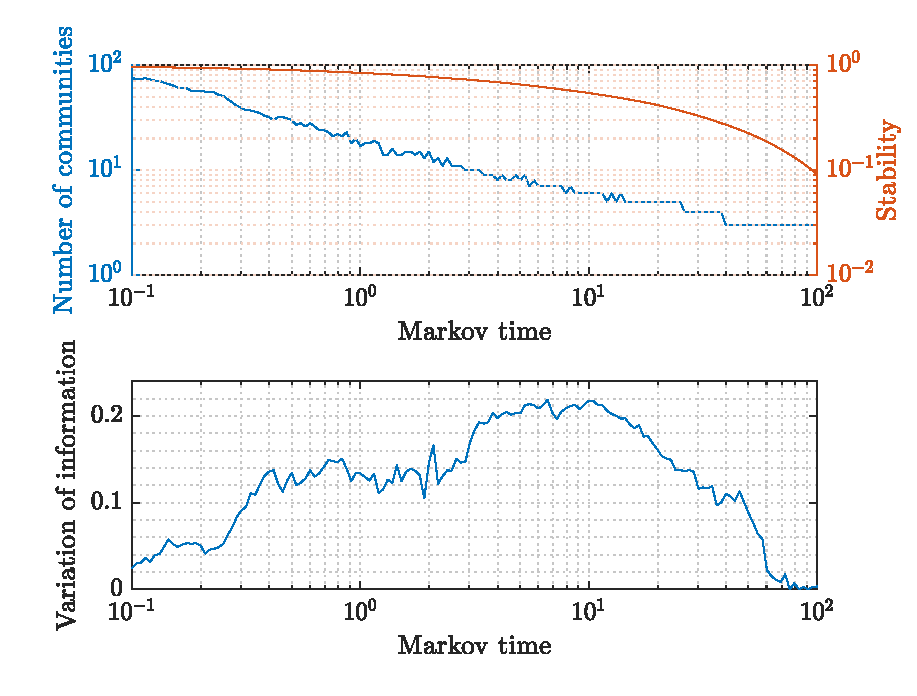
\includegraphics[width = .7\textwidth]{clusters/stab0.eps}
	\caption{Stability, number of communities and variation of information as a function of the Markov time for $T=1$ year.}
	\label{fig:stab0}
\end{figure}

\begin{figure}[H]
	\centering
	\begin{subfigure}[t]{0.49\textwidth}
		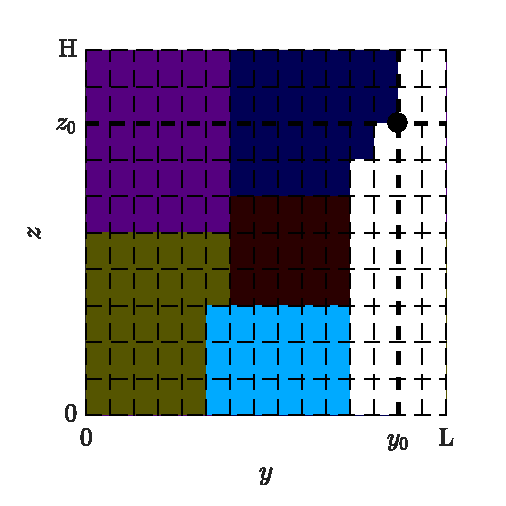
\includegraphics[width=\textwidth]{clusters/cluster0_6_.eps}
		\caption{6 communities.}
		\label{fig:cluster0_6_}
	\end{subfigure}
	\begin{subfigure}[t]{0.49\textwidth}
		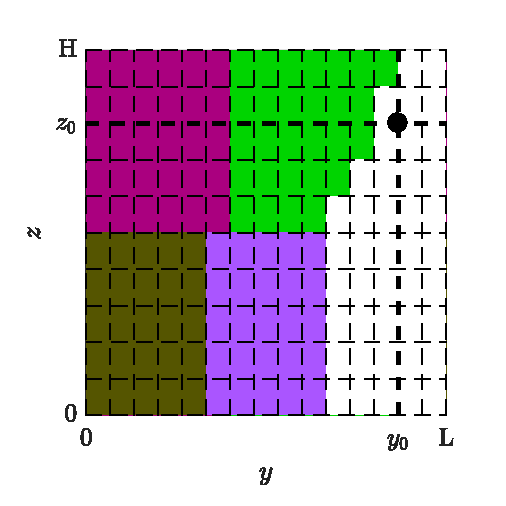
\includegraphics[width=\textwidth]{clusters/cluster0_5_.eps}
		\caption{5 communities.}
		\label{fig:cluster0_5_}
	\end{subfigure}
	\begin{subfigure}[t]{0.49\textwidth}
		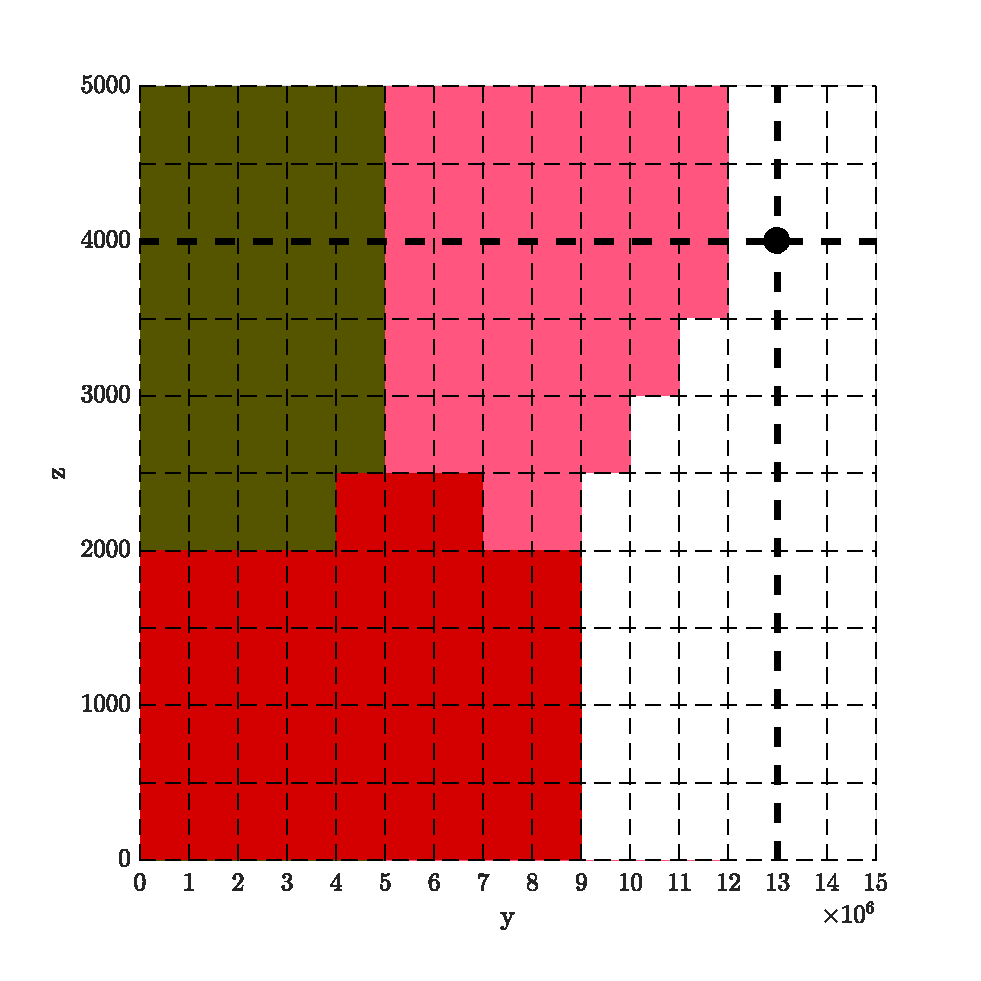
\includegraphics[width=\textwidth]{clusters/cluster0_4_.eps}
		\caption{4 communities.}
		\label{fig:cluster0_4_}
	\end{subfigure}
	\begin{subfigure}[t]{0.49\textwidth}
		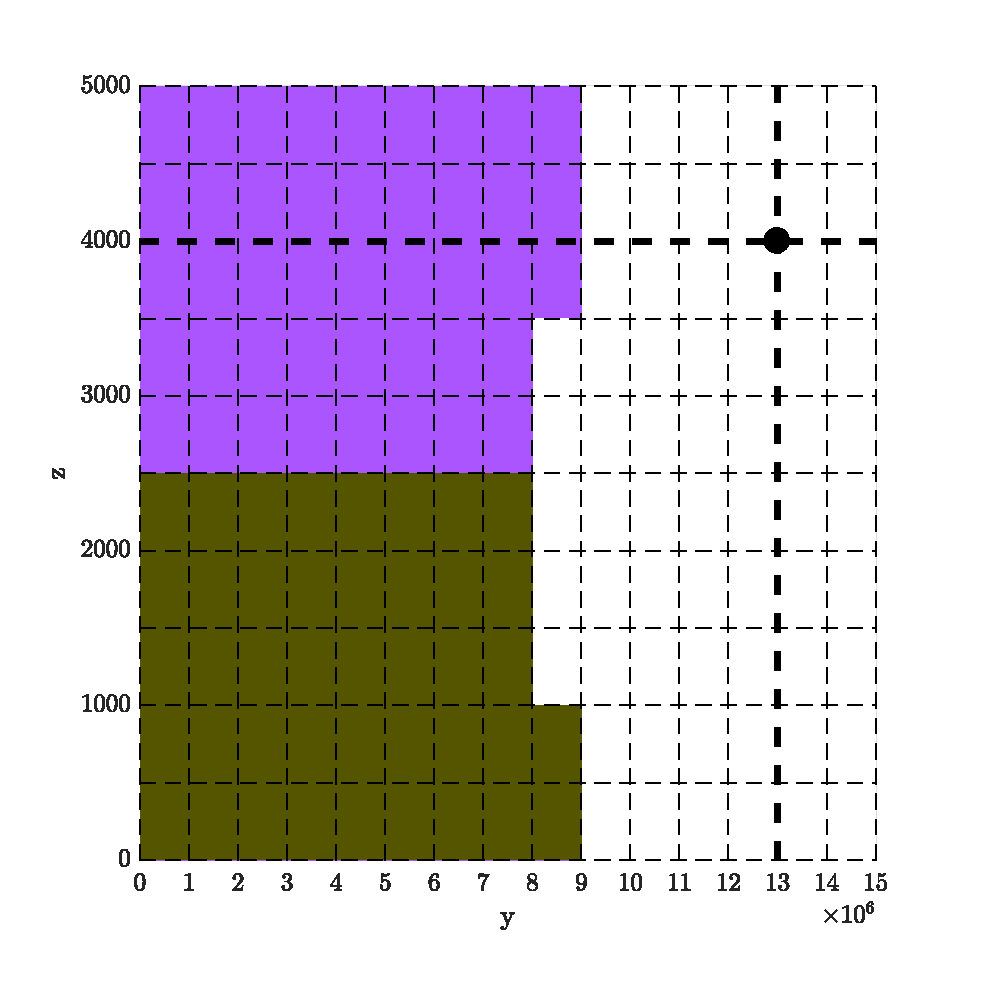
\includegraphics[width=\textwidth]{clusters/cluster0_3_.eps}
		\caption{3 communities.}
		\label{fig:cluster0_3_}
	\end{subfigure}
	\caption{The relevant clusterings detected at different time scales for $T=1$ year.}
	\label{fig:cluster0}
\end{figure}

%------------------ T = 10 -----------------------------%

\begin{figure}[H]
	\centering
	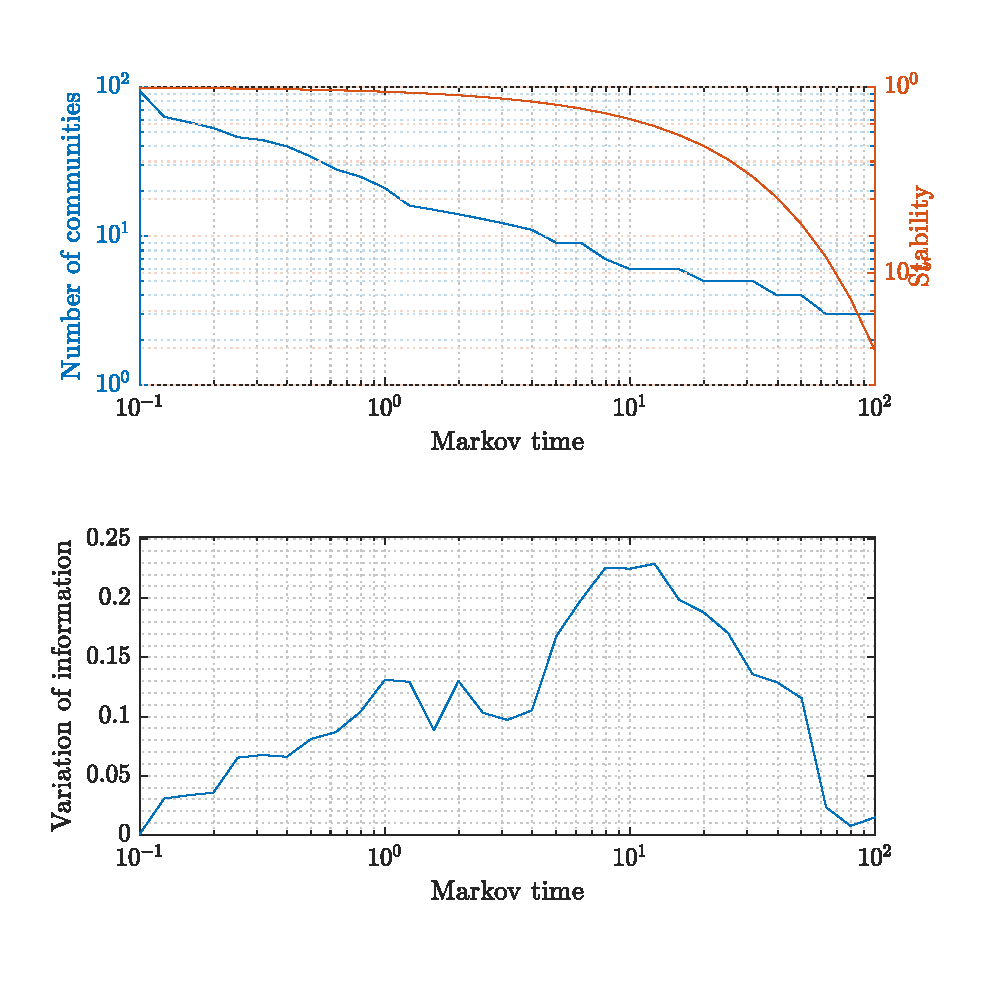
\includegraphics[width = .7\textwidth]{clusters/stab1.eps}
	\caption{Stability, number of communities and variation of information as a function of the Markov time for $T=10$ years.}
	\label{fig:stab1}
\end{figure}

\begin{figure}[H]
	\centering
	\begin{subfigure}[t]{0.49\textwidth}
		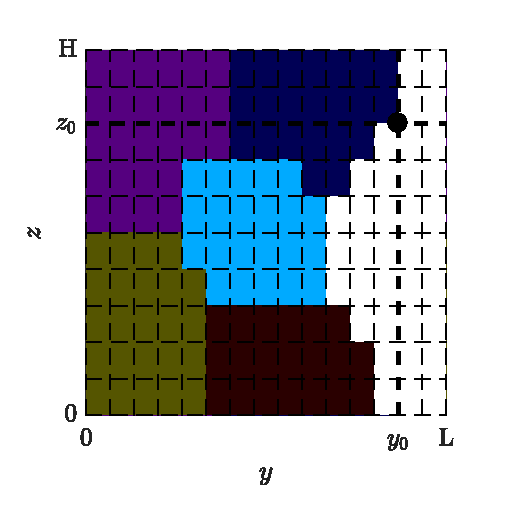
\includegraphics[width=\textwidth]{clusters/cluster1_6_.eps}
		\caption{6 communities.}
		\label{fig:cluster1_6_}
	\end{subfigure}
	\begin{subfigure}[t]{0.49\textwidth}
		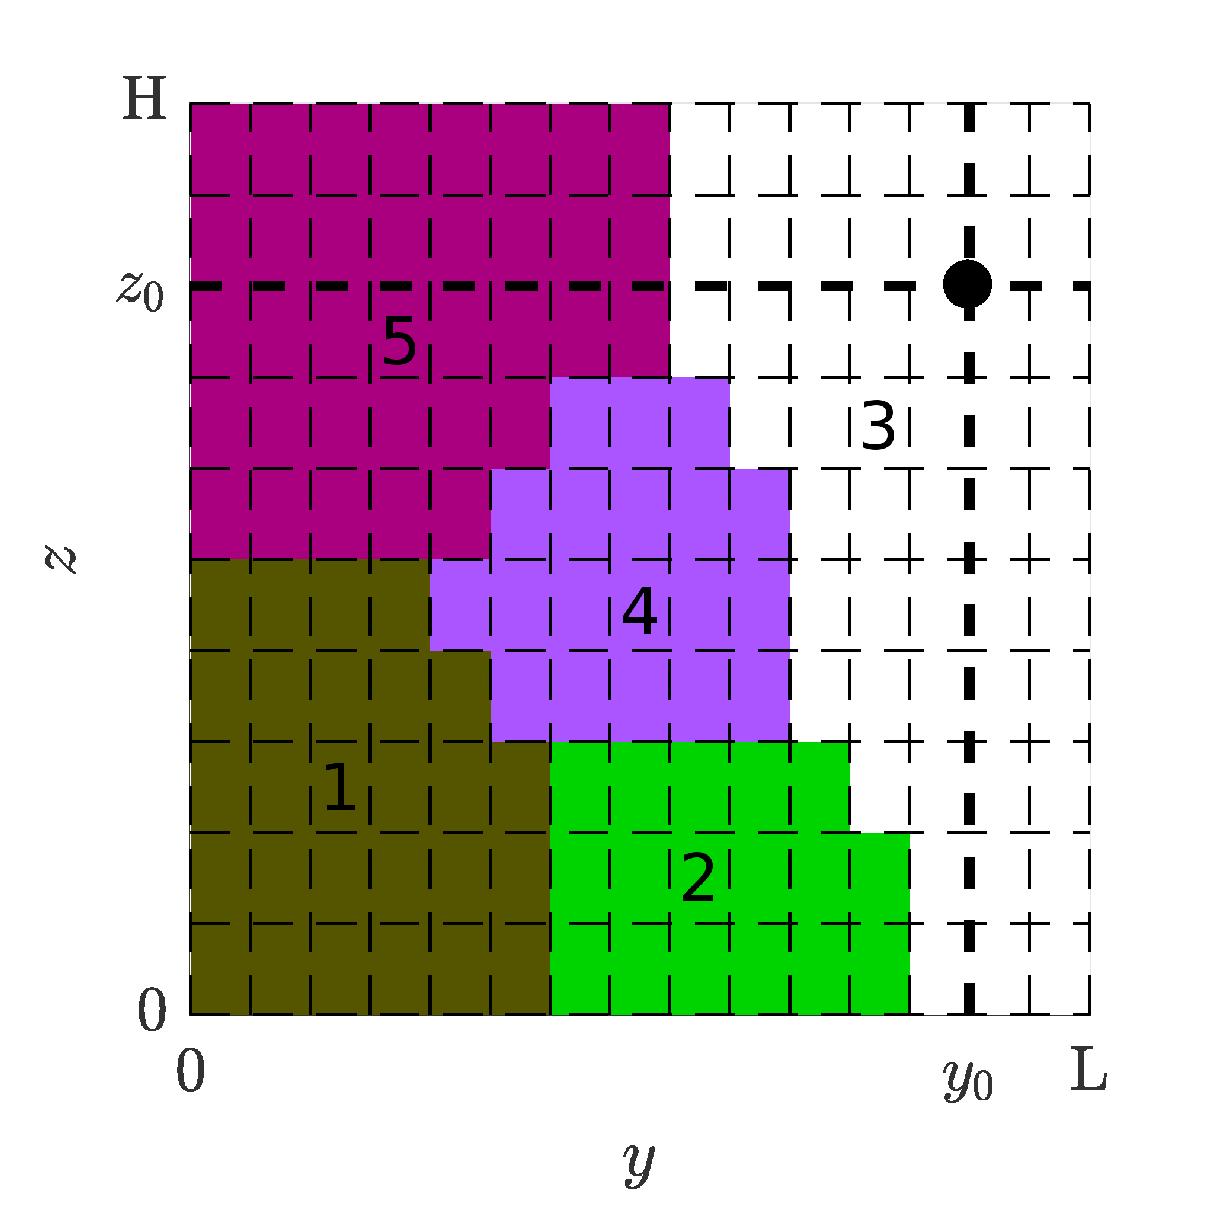
\includegraphics[width=\textwidth]{clusters/cluster1_5_num.eps}
		\caption{5 communities.}
		\label{fig:cluster1_5_}
	\end{subfigure}
	\begin{subfigure}[t]{0.49\textwidth}
		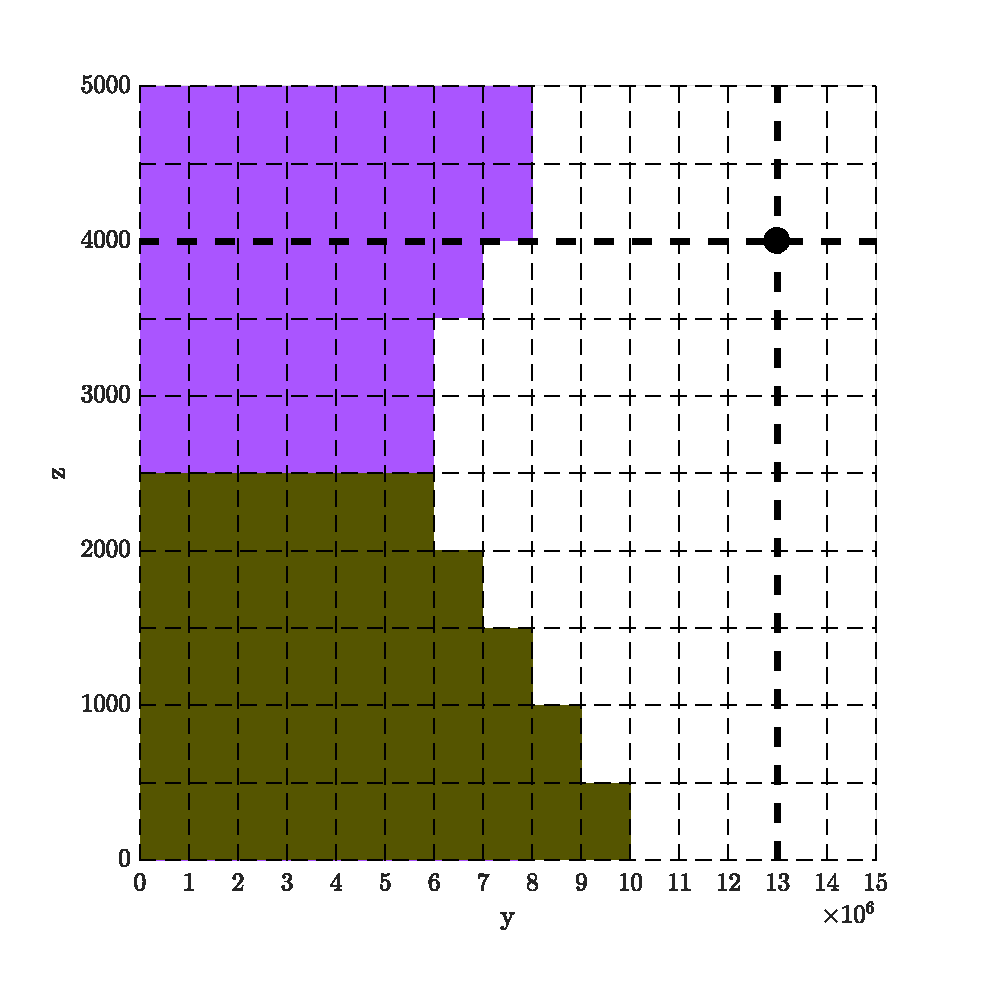
\includegraphics[width=\textwidth]{clusters/cluster1_3_.eps}
		\caption{3 communities.}
		\label{fig:cluster1_3_}
	\end{subfigure}
	\begin{subfigure}[t]{0.49\textwidth}
		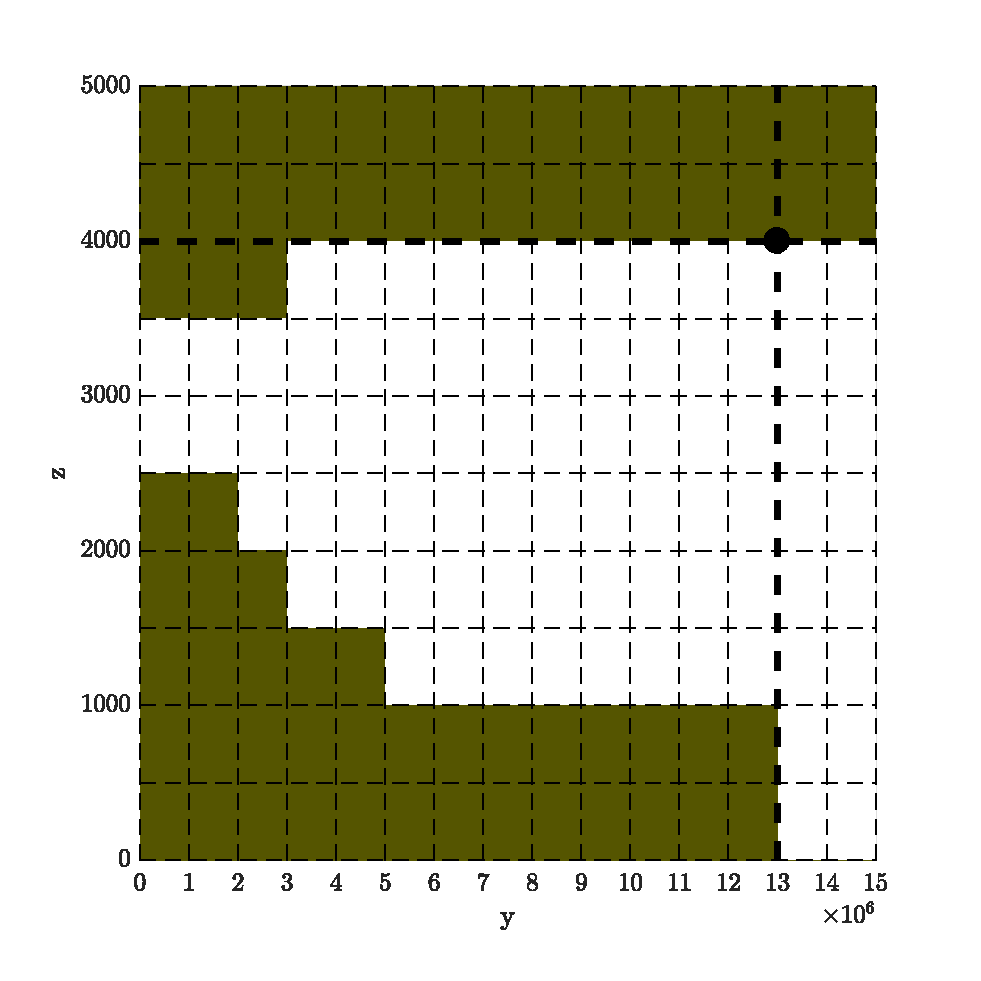
\includegraphics[width=\textwidth]{clusters/cluster1_2_.eps}
		\caption{2 communities detected by the algorithm which should rather be considered as being 3 communities.}
		\label{fig:cluster1_2_}
	\end{subfigure}
	\caption{The relevant clusterings detected at different time scales for $T=10$ years.}
	\label{fig:cluster1}
\end{figure}

%------------------ T = 50 -----------------------------%
\begin{figure}[H]
	\centering
	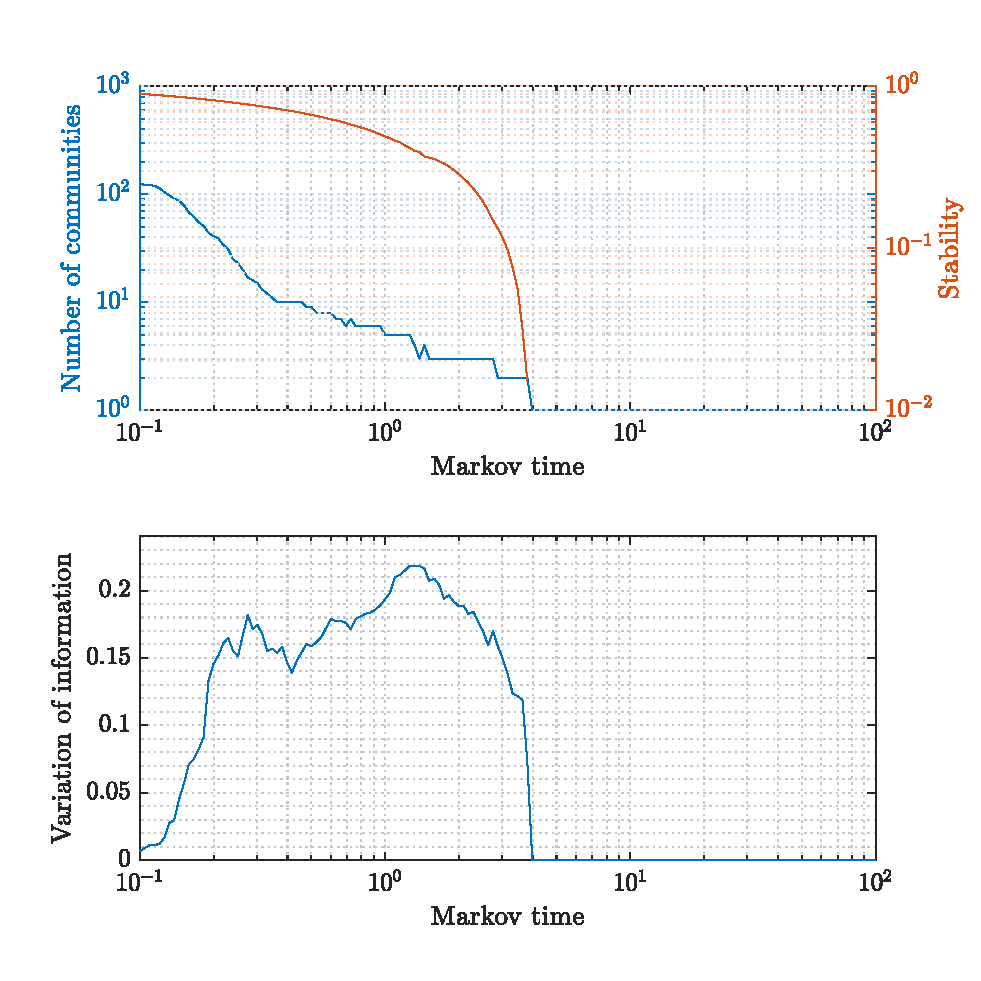
\includegraphics[width = .7\textwidth]{clusters/stab5.eps}
	\caption{Stability, number of communities and variation of information as a function of the Markov time for $T=50$ years.}
	\label{fig:stab5}
\end{figure}

\begin{figure}[H]
	\centering
	\begin{subfigure}[t]{0.49\textwidth}
		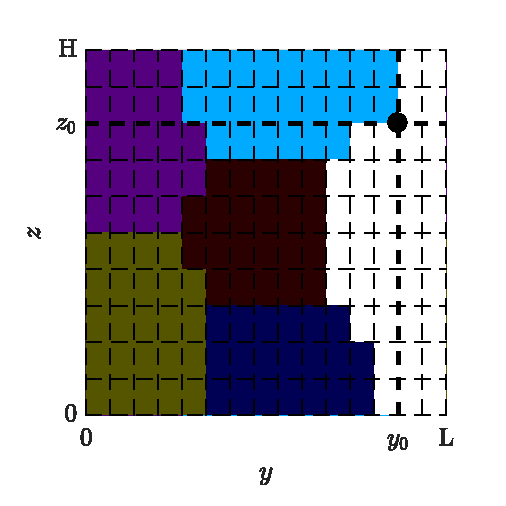
\includegraphics[width=\textwidth]{clusters/cluster5_6_.eps}
		\caption{6 communities.}
		\label{fig:cluster5_6_}
	\end{subfigure}
	\begin{subfigure}[t]{0.49\textwidth}
		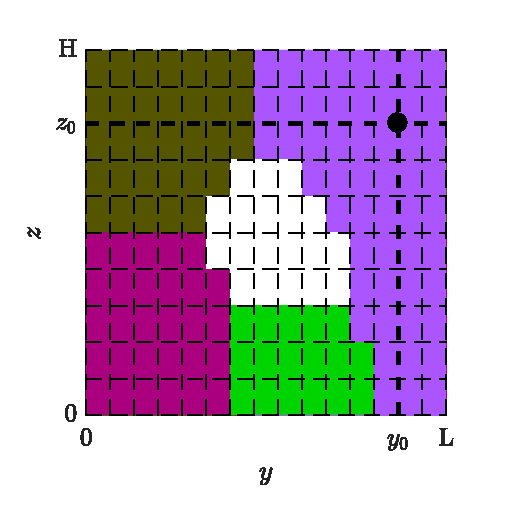
\includegraphics[width=\textwidth]{clusters/cluster5_5_.eps}
		\caption{5 communities.}
		\label{fig:cluster5_5_}
	\end{subfigure}
	\begin{subfigure}[t]{0.49\textwidth}
		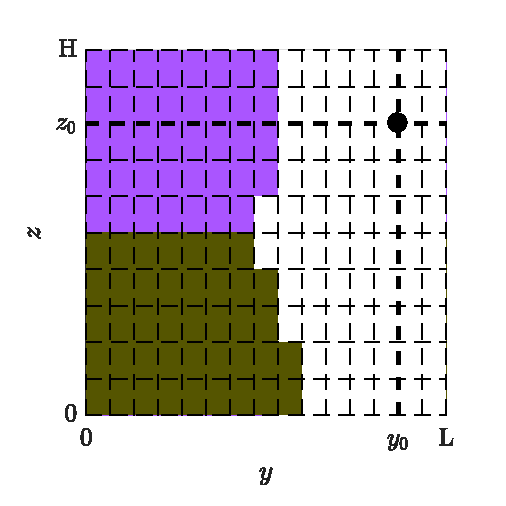
\includegraphics[width=\textwidth]{clusters/cluster5_3_.eps}
		\caption{3 communities.}
		\label{fig:cluster5_3_}
	\end{subfigure}
	\begin{subfigure}[t]{0.49\textwidth}
		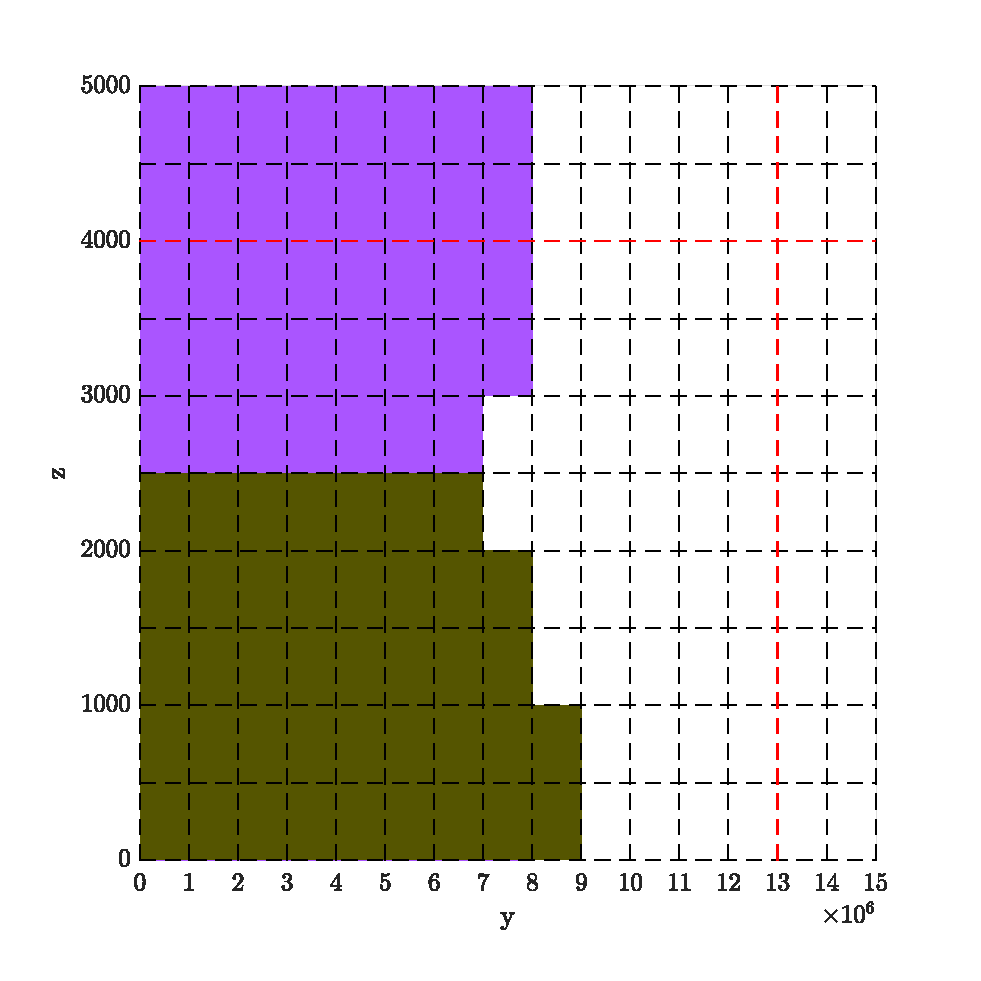
\includegraphics[width=\textwidth]{clusters/cluster5_2_.eps}
		\caption{2 communities.}
		\label{fig:cluster5_2_}
	\end{subfigure}
	\caption{The relevant clusterings detected at different time scales for $T=50$ years.}
	\label{fig:cluster5}
\end{figure}

%------------------ T = 100 ----------------------------%
\begin{figure}[H]
	\centering
	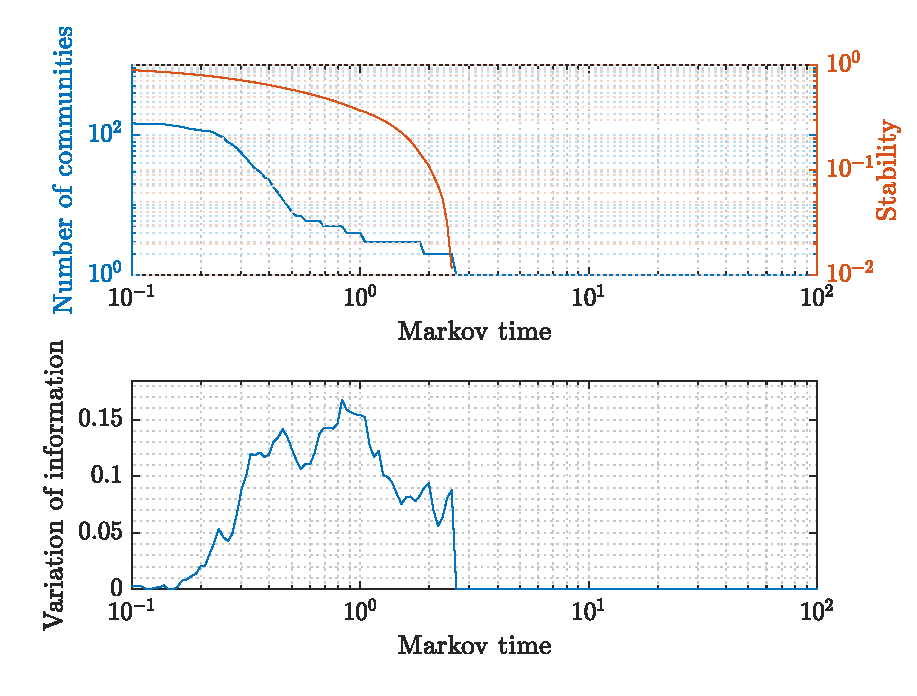
\includegraphics[width = .7\textwidth]{clusters/stab10.eps}
	\caption{Stability, number of communities and variation of information as a function of the Markov time for $T=100$ years.}
	\label{fig:stab10}
\end{figure}

\begin{figure}[H]
	\centering
	\begin{subfigure}[t]{0.49\textwidth}
		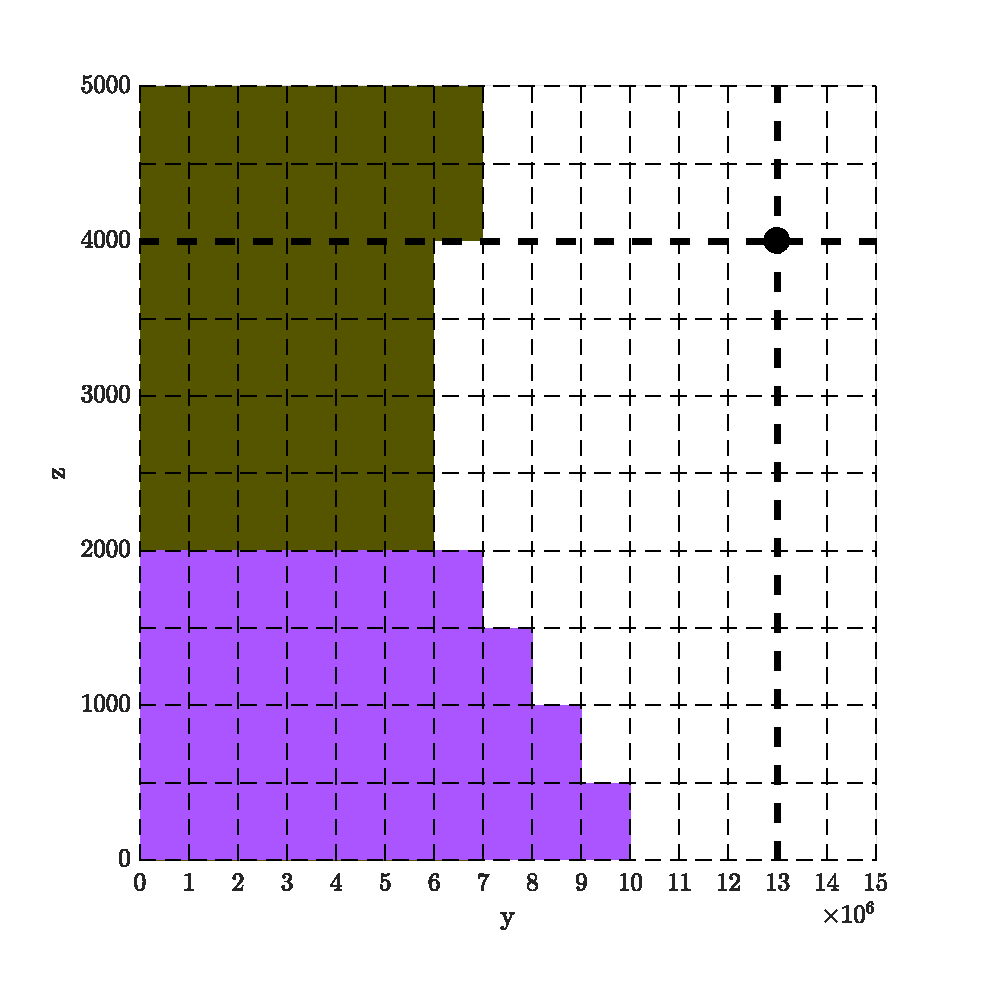
\includegraphics[width=\textwidth]{clusters/cluster10_3_.eps}
		\caption{3 communities.}
		\label{fig:cluster10_3_}
	\end{subfigure}
	\begin{subfigure}[t]{0.49\textwidth}
		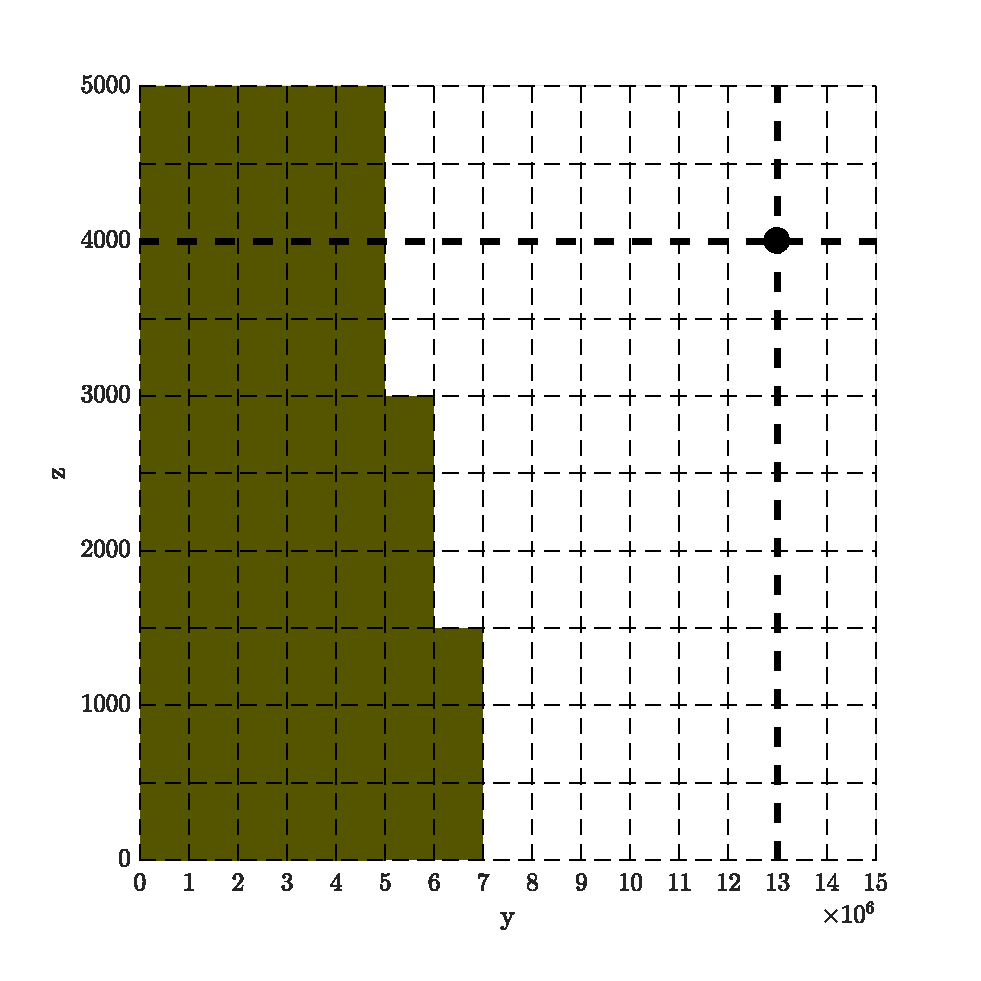
\includegraphics[width=\textwidth]{clusters/cluster10_2_.eps}
		\caption{2 communities.}
		\label{fig:cluster10_2_}
	\end{subfigure}
	\caption{The relevant clusterings detected at different time scales for $T=100$ years.}
	\label{fig:cluster10}
\end{figure}

\part{Applications}
%!TEX root = /home/renaud/Documents/EPL/tfe/latex/tfe.tex
\chapter{The "overturner" circulation model} \label{chap:overturnercirculation}
A velocity field is proposed here that will be used further to build problems on which the method will be applied. That circulation model was initially proposed by \textit{E. Deleersnijder} \cite{deleersnijder2006overturner} as an idealized, two-dimensional representation of the meridian circulation in the Atlantic ocean. It has been studied extensively by \textit{C. Timmermans} in her master's thesis \cite{timmermans2006masterthesis}. The justifications of the model can be found in the latter. In this chapter, we only present the circulation model without justification. 
%\textcolor{red}{Soit on fait le modèle overturner plus loin et alors il faut des justifications. Soit on ne le fait pas et c'est ok.}

\section{An idealized velocity field}
Let us consider a rectangular domain in the $(y,z)$-coordinate system. 
%The coordinate $y$ is associated to the latitude with $\hat{\b{e}}_y$ pointing towards the North, and $z$ is associated to the depth with $\hat{\b{e}}_z$ pointing upwards. 
The domain $\Omega$ is delimited by
\begin{equation} 
	0 \le y \le L,\quad 0 \le z \le H,
\end{equation}
where $L$ and $H$ are positive constants. 
%The ocean surface is thus located at $z = H$ while $z = 0$ stands for the deep-ocean. The South and North boundaries are respectively given by $y = 0$ and $y = L$. We aim at defining a stationary velocity field $\b u(y,z) = (v(y,z),\, w(y,z))$ that would roughly reproduce the main qualitative features of the meridian circulation in the Atlantic ocean. Under the Boussinesq approximation, the continuity equation reads
The stationary velocity field is denoted $\b u(y,z) = (v(y,z),\, w(y,z))$. Under the Boussinesq approximation, the continuity equation reads
\begin{equation} \label{eq:continuity_boussinesq}
	\nabla \cdot \b u = 0,
\end{equation}
For our particular problem, this amounts to
\begin{equation}
	\frac{\partial v}{\partial y} + \frac{\partial w}{\partial z} = 0.
\end{equation}
No-through boundary conditions are imposed at the boundaries of the domain, which implies that $\b u(y,z) \cdot \hat{\b{n}} = 0$ everywhere on $\partial \Omega$ (where $\hat{\b{n}}$ is the outwards unit normal at the boundary), or equivalently :
\begin{equation} \label{eq:overturnerBC}
	v(0,z) = 0, \quad v(L,z) = 0, \quad w(y,0) = 0 \quad \mbox{and} \quad w(y,H) = 0.
\end{equation}
%\textcolor{red}{Blahblah à mettre en relation avec ce qu'on doit dire plus tôt sur les modèles 2D de l'océan Atlantique,... Éventuellement s'inspirer de Timmermans mais attention quand même...}

In order to build a velocity field that satisfies the continuity equation~\eqref{eq:continuity_boussinesq}, a \textit{streamfunction} approach is used. The whole approach is explained in appendix~\ref{app:streamfunction} along with some important properties of the streamfunction in two dimensions that will be useful in the next. Let $\psi$ denote the streamfunction. The velocity field satisfies the relation
\begin{equation}
	\b u = - \rot \psi.
\end{equation}
In particular, $\psi$ must be such that the boundary conditions~\eqref{eq:overturnerBC} are satisfied. Those conditions state that $\b u$ must be tangent to the boundary everywhere on $\partial \Omega$, which precisely amounts to require that $\psi$ is constant on $\partial \Omega$ (see property~\ref{prop:streamfunction-tangent}). Without loss of generality, we can choose this constant to be zero. Hence, we require that 
\begin{equation}
	\psi(0,z) = 0, \ \psi(L,z) = 0, \ \psi(y,0) = 0 \ \mbox{and} \ \psi(y,H) = 0,\ \mbox{for all $(y,z) \in \Omega$}.
\end{equation}

%\textcolor{red}{Faire des liens avec chapitre précédent} 
In order to build an acceptable idealization of the meridian circulation in the Atlantic ocean, \textit{Deleersnijder} proposes in his working paper \cite{deleersnijder2006overturner} to suppose that the meridian streamfunction has a unique extremum $\Psi$, which is a maximum, and that it reaches that maximum at the point of coordinates $(y_0,z_0)$, located near the surface and near the North boundary of the domain. It is important to recall that the second partial derivatives of $\psi$ must exist and be continuous for the above relations to hold.

Let $\xi_0 \in \mathbb{R}_0^+$, and let $\phi(\xi,\xi_0)$ be defined as
\begin{equation} \label{eq:phi}
	\phi(\xi,\xi_0) = \frac{\xi(2\xi_0-\xi)}{\xi_0^2},
\end{equation}
The derivative $\phi'(\xi,\xi_0)$ of $\phi$ with respect to $\xi$ is
\begin{equation}
	\phi'(\xi,\xi_0) = \frac{2(\xi_0-\xi)}{\xi_0^2}.
\end{equation}
An expression of the meridian streamfunction that satisfies the above constraints is then
\begin{equation} \label{eq:psi_overturner}
	\psi(y,z) = \Psi\left\{ 
		\begin{array}{lrrr}
			\phi(y,y_0)\phi(z,z_0) & \mbox{if} & 0 \le y < y_0, & 0 \le z < z_0,\\
			\phi(y,y_0)\phi(H-z,H-z_0) & \mbox{if} & 0 \le y < y_0, & z_0 < z \le H,\\
			\phi(L-y,L-y_0)\phi(H-z,H-z_0) & \mbox{if} & y_0 < y \le L, &z_0 < z \le H,\\
			\phi(L-y,L-y_0)\phi(z,z_0) & \mbox{if} & y_0 < y \le L, & 0 \le z < z_0,\\
			\phi(z,z_0) & \mbox{if} & y = y_0, & 0 \le z < z_0,\\
			\phi(H-z,H-z_0) & \mbox{if} & y = y_0, & z_0 < z \le H,\\
			\phi(y,y_0) & \mbox{if} & 0 \le y < y_0, & z = z_0,\\
			\phi(L-y,L-y_0) & \mbox{if} & y_0 < y \le L, & z=z_0,\\
			1 & \mbox{if} & y = y_0, & z=z_0.\\
		\end{array}
	\right.
\end{equation}
Figure~\ref{fig:psi_overturner} shows the isolines of the adimensional streamfunction $\psi/\Psi$ for a given choice of the parameters. The point is that this circulation describes revolutions around the point $(y_0,z_0)$. With the choice $\b u = - \nabla \times \psi$, those revolutions are clockwise.
\begin{figure}[!htp]
	\centering
	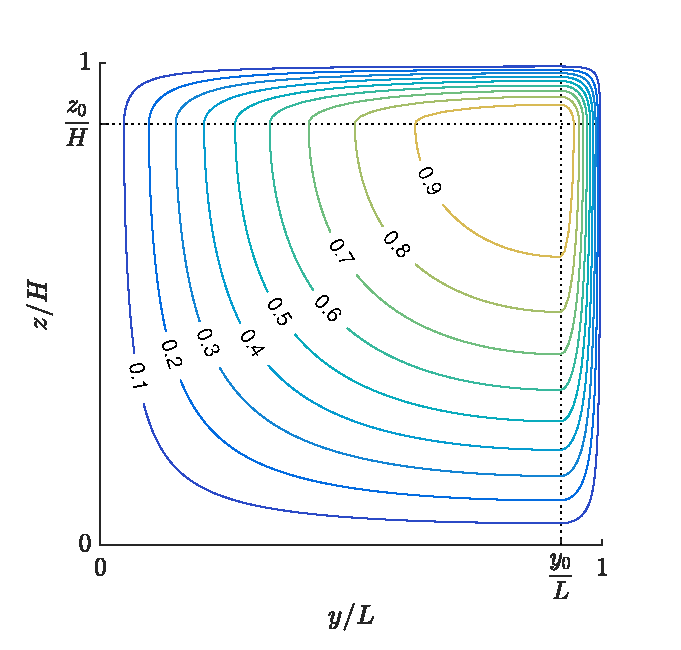
\includegraphics[width=.5\textwidth]{fig/overturner/psi.eps}
	\caption{Some isolines of the adimensional meridian streamfunction $\psi(y,z)/\Psi$, which are also streamlines of the flow.}
	\label{fig:psi_overturner}
\end{figure}

The meridian and vertical components of the velocity are then expressed as
\begin{equation} \label{eq:v_overturner}
	v(y,z) = \Psi\left\{ 
		\begin{array}{lrrr}
			- \phi(y,y_0)\phi'(z,z_0) & \mbox{if} & 0 \le y < y_0, & 0 \le z < z_0,\\
			\phi(y,y_0)\phi'(H-z,H-z_0) & \mbox{if} & 0 \le y < y_0, & z_0 < z \le H,\\
			\phi(L-y,L-y_0)\phi'(H-z,H-z_0) & \mbox{if} & y_0 < y \le L, & z_0 < z \le H,\\
			- \phi(L-y,L-y_0)\phi'(z,z_0) & \mbox{if} & y_0 < y \le L, & 0 \le z < z_0,\\
			- \phi'(z,z_0) & \mbox{if} & y = y_0, & 0 \le z < z_0,\\
			\phi'(H-z,H-z_0) & \mbox{if} & y = y_0, & z_0 < z \le H,\\
			0 & \mbox{if} &0 \le y \le L, & z = z_0.
		\end{array}
	\right.
\end{equation}
and
\begin{equation} \label{eq:w_overturner}
	w(y,z) = \Psi\left\{ 
		\begin{array}{lrrr}
			\phi'(y,y_0)\phi(z,z_0) & \mbox{if} & 0 \le y < y_0, & 0 \le z < z_0,\\
			\phi'(y,y_0)\phi(H-z,H-z_0) & \mbox{if} & 0 \le y < y_0, & z_0 < z \le H,\\
			- \phi'(L-y,L-y_0)\phi(H-z,H-z_0) & \mbox{if} & y_0 < y \le L, & z_0 < z \le H,\\
			- \phi'(L-y,L-y_0)\phi(z,z_0) & \mbox{if} & y_0 < y \le L, & 0 \le z < z_0,\\
			\phi'(y,y_0) & \mbox{if} & 0 \le y < y_0, & 0 \le z = z_0,\\
			- \phi'(L-y,L-y_0) & \mbox{if} & y_0 < y \le L, & z = z_0,\\
			0 & \mbox{if} & y = y_0. &
		\end{array}
	\right.
\end{equation} % Attention, a priori cette section va disparaitre. Mais plusieurs références ! Les rediriger
%!TEX root = /home/renaud/Documents/EPL/tfe/latex/tfe.tex
\chapter{Application: the bi-overturner problem}

%!TEX root = /home/renaud/Documents/EPL/tfe/latex/tfe.tex
\section{Application of the method on a simple class of problems}
This section can be considered as a kind of \textit{sanity check} of the method: we define a class of problems for which the box decomposition is intuitively obvious and we check that a community detection algorithm applied on the problem allows to find back that box-decomposition. We call that class of problems the \textit{bi-overturner} problems. The domain that we consider is $\Omega = [-L,\,L]\times[0,\,H]$. Bi-overturner problems basically consist of two \textit{overturner-like} circulations models side-by-side. Let $\Omega^- = [-L,\,0[\times[0,\,H]$ and $\Omega^+ =\; ]0,\,L]\times[0,\,H]$. If $\psi(y,z;y_0,z_0)$ denote the streamfunction defined in \eqref{eq:psi_overturner} with parameters $y_0 \in\; ]0,\,L[$ and $z_0 \in\; ]0,\,H[$, then the streamfunction $\psi_2$ of the bi-overturner problems is defined as
\begin{equation} \label{eq:psi_2box}
	\psi_2(y,z) = \left\{ 
		\begin{array}{lrr}
			\psi(L+y,z;y_0,z_0) & \mbox{if} & (y,z) \in \Omega^-,\\
			0 & \mbox{if} & (y,z) \in \{(0,z)\;|\;z \in [0,\,H]\},\\
			-\psi(y,z;L-y_0,z_0) & \mbox{if} & (y,z) \in \Omega^+,\\
		\end{array}
	\right.
\end{equation}
The streamfunction $\psi_2$ has two extrema of equal strengths: a maximum at $(y_0^-,z_0)$ with $y_0^- \triangleq -L+y_0 = -y_0^-$ and a minimum at $(y_0^+,z_0)$ with $y_0^+ \triangleq L-y_0$. The overturner-like circulation is clockwise in $\Omega^-$ and counterclockwise in $\Omega^+$. The horizontal and vertical velocities $v$ and $w$ are given by
\begin{equation} \label{eq:u-psi_2box}
	v = -\frac{\partial \psi_2}{\partial z}, \quad w = \frac{\partial \psi_2}{\partial y}.
\end{equation}
 Isolines are shown in figures \ref{fig:v2box} and \ref{fig:w2box} respectively. The key feature is that $v(0,z) = 0$, namely the horizontal velocity is zero on the whole segment $y = 0$. Hence, if there is no horizontal diffusion, a passive tracer's particle starting in $\Omega^-$ can never reach $\Omega^+$ and conversely. In that case, we can imagine that there is a vertical wall implying no-through boundary conditions at $y=0$ and the graph is not ergodic. But if the horizontal diffusivity is nonzero in some area near $y=0$, then exchange of particles between $\Omega^-$ and $\Omega^+$ can happen in that area. Now we suppose that the diffusivity tensor $\b K$ is diagonal:
 \begin{equation}
 	\b K(y,z) = \begin{pmatrix} K_h(y,z) & 0\\ 0 & K_v \end{pmatrix}.  	
 \end{equation} 
We assume that the vertical diffusivity $K_v$ is constant and equal to $10^{-3}$ [$\rm{m^2/s}$]. Now we introduce the parameter $\alpha \in [0,1]$ and define $z^* = \alpha H$. We choose an horizontal diffusivity $K_h$ of the form
\begin{equation} \label{eq:Kh2box}
	K_h(y,z) = \begin{cases}
			10^4\ \rm{[m^2/s]} & \mbox{if} \quad y_0^- \le y \le y_0^+ \quad \mbox{and} \quad z^* \le z \le H,\\
			10^3\ \rm{[m^2/s]} & \mbox{if} \quad -L \le y < y_0^- \quad \mbox{or} \quad y_0^+ < y \le L,\\
			0\ \rm{[m^2/s]}  & \mbox{otherwise}.
		\end{cases}
\end{equation}
Now, exchange between $\Omega^-$ and $\Omega^+$ is possible but only above $z^*$.\footnote{From a numerical, random-walk, point of view, we should also ensure that $y_0^+ = |y_0^-|$ is sufficiently large. If not, it would be numerically possible for particles lying below $z^*$ and before $y_0^-$ (resp. after $y_0^+$) to jump from $\Omega^-$ (resp. $\Omega^+$) to $\Omega^+$ (resp. $\Omega^-$).} For the next, we call \textit{exchange zone} the area where $K_v = 10^4$ $\rm{[m^2/s]}$ (dark gray zone in figure \ref{fig:Kh2box}) Hence, we can imagine that there is a vertical, no-through wall of height $z^*$ at $y=0$. The situation is depicted on figure \ref{fig:Kh2box}. Making $\alpha$ vary between $0$ and $1$ defines a class of bi-overturner problem where the vertical wall's height $z^*$ at $y=0$ vary between $0$ and $H$. Two examples of trajectories with the same initial condition are shown for $\alpha = 0.75$ in figures \ref{fig:withouttransfer} and \ref{fig:withtransfer}.

\begin{figure}[!htp]
	\centering
	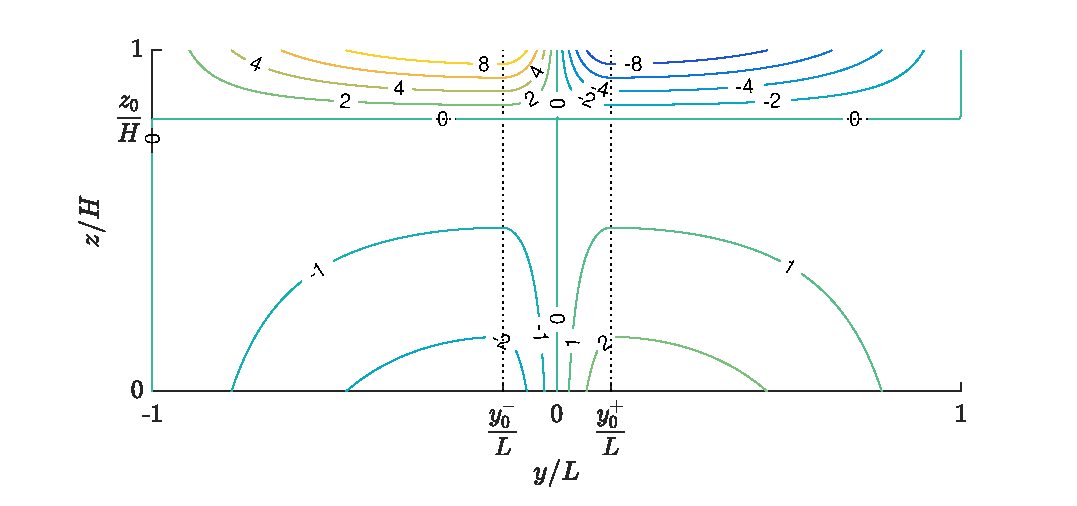
\includegraphics[width=\textwidth]{fig/problem2box/v2box_timmermans.eps}
	\caption{Isolines of the horizontal velocity $v$ for bi-overturner problems.}
	\label{fig:v2box}
\end{figure}

\begin{figure}[!htp]
	\centering
	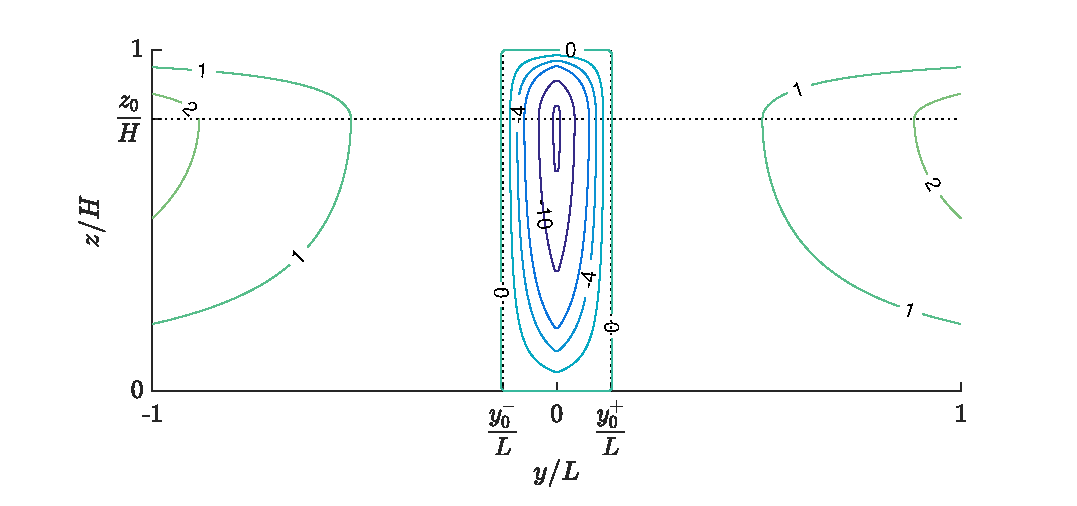
\includegraphics[width=\textwidth]{fig/problem2box/w2box_timmermans.eps}
	\caption{Isolines of the horizontal velocity $w$ for bi-overturner problems.}
	\label{fig:w2box}
\end{figure}

\begin{figure}[!htp]
	\centering
	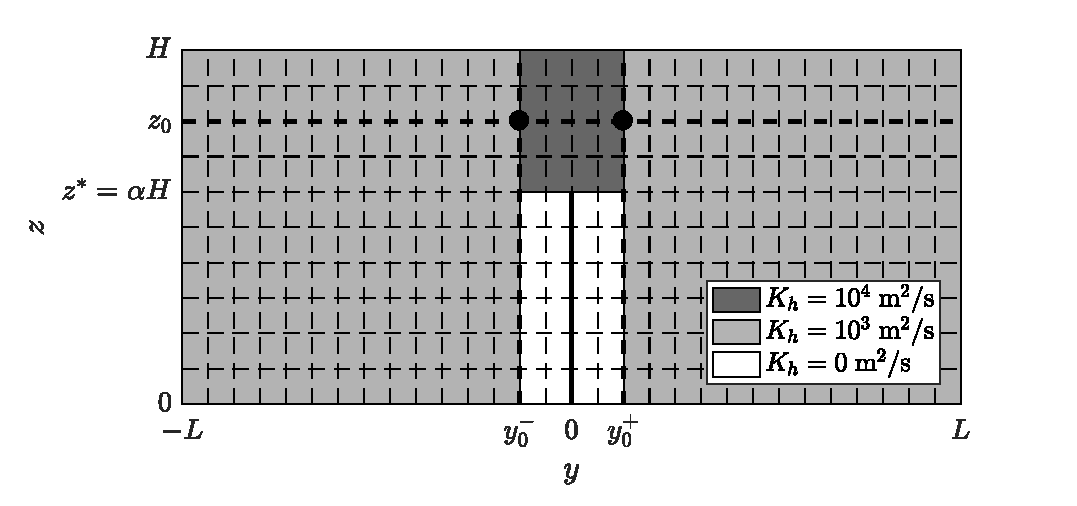
\includegraphics[width=\textwidth]{fig/problem2box/problem.eps}
	\caption{Illustration of the decomposition of the domain into boxes corresponding to the nodes of the directed graph. The values of $K_h$ are also shown for $\alpha = 0.6$, and the fictitious wall is represented by the black continuous line. Here the particle enters the exchange zone but finally stays in $\Omega^-$.}
	\label{fig:Kh2box}
\end{figure}

\begin{figure}[!htp]
	\centering
	\includegraphics[width=\textwidth]{fig/problem2box/traj_without_transfer5.eps}
	\caption{Example of a particle trajectory in the bi-overturner model with $\alpha = 0.75$. The black cross represents the initial position whereas the black dot shows the final position. The simulation time is 200 years.}
	\label{fig:withouttransfer}
\end{figure}

\begin{figure}[!htp]
	\centering
	\includegraphics[width=\textwidth]{fig/problem2box/traj_with_transfer2.eps}
	\caption{Example of a particle trajectory in the bi-overturner model with $\alpha = 0.75$. The black cross represents the initial position whereas the black dot shows the final position. The simulation time is 200 years.}
	\label{fig:withtransfer}
\end{figure}
When $\alpha = 1$, the obvious compartmental model is made of the two compartments $\Omega^-$ and $\Omega^+$ which do not communicate with each other. Suppose that different amounts of passive tracer are released into $\Omega^-$ and $\Omega^+$ at a given time; the concentration in each compartment tends to become uniform in time due to diffusion, but the concentration in $\Omega^-$ depends only on the initial quantity of tracer released in $\Omega^-$ and similarly for the concentration in $\Omega^+$. At the contrary, when $\alpha = 0$ the concentration tends to become uniform over the whole domain when time goes to infinity. Hence, we can expect three types of partitioning: a three-communities partitioning with left and right compartments and an exchange zone in between; a two-communities partitioning corresponding to $\Omega^-$ and $\Omega^+$; and finally a trivial partitioning with one single community for very long time scales. For intermediate values of $\alpha$, we expect a behavior similar to the case $\alpha = 1$ when $\alpha$ is close to $1$ and similar to the case $\alpha = 0$ when $\alpha$ goes to $0$. 

\subsection{Results}
The partitioning results are presented here for $\alpha = 1$, $\alpha = 0.75$, $\alpha = 0.5$, $\alpha = 0.25$ and $\alpha = 0$. For every value of $\alpha$, the transition probability matrix is computed at $T = 1$ year on a discretization like the one presented in figure \ref{fig:Kh2box}, namely with $\nby = 30$ and $\nbz = 10$. $10\,000$ particles are initially released in every box. The stability software is run using a vector of Markov times taking values between $10$ and $10^3$. Since we have computed the transition probability matrix for $T = 1$ year, one unit of Markov time correspond here to one year. Notice that in the case where $\alpha = 1$, the graph is not ergodic (it is composed of two ergodic classes) and a random teleportation probability \mtlb{tau} $= 10^{-3}$ is used when running the stability software. When $\alpha < 1$, \mtlb{tau} $=0$ is used.
The stability, number of communities and variation of information curves are shown in figures \ref{fig:staba1}, \ref{fig:staba75}, \ref{fig:staba5}, \ref{fig:staba25} and \ref{fig:staba0} for different values of $\alpha$. Most robust communities correspond to plateaux in the community curve together with a low variation of information. Whatever the value of $\alpha$, the number of communities goes to $2$ after maximum $50$ years, together with a variation of information that is almost zero. In every case, the two-communities partitioning corresponds as expected to $\Omega^-$ and $\Omega^+$. It is shown in figure \ref{fig:cluster_a25_2} for the case $\alpha = 0.25$. In that case, the boundary is perfectly straight which corresponds to the intuition and is conform to the remark made on page \pageref{remark:straightboundaries}. In some other cases, like when $\alpha = 0.5$, the boundary is not exactly a straight line. The situation is depicted in figure \ref{fig:cluster_a5_2}. However, we have to remember that neither the transition probability matrix nor the stability partitioning is solved exactly. Hence, we can consider that the irregularity in the boundary of the communities is due to those numerical artifacts: if a box-model has to be build from the partitioning shown in figure \ref{fig:cluster_a5_2}, the compartments should of course be chosen with a vertical boundary. This illustrates the fact that when using a community-detection algorithm to build compartments for a box-model, the communities should not be blindly interpreted as being the relevant compartments. In particular, if the boundaries of the communities are almost but not exactly vertical and horizontal, one should consider straight boundaries for the compartments. Community detection should thus be considered as a guide towards choosing relevant compartments, rather than as an exact method.

When $\alpha = 0.75$, a small three-communities plateaux starts appearing around 40 years. This plateau grows as $\alpha$ decreases. The corresponding clusterings are shown in figures \ref{fig:cluster_a25_3} and \ref{fig:cluster_a0_3}, where a community corresponding to the exchange zone appears, as expected.

In figure \ref{fig:staba0} corresponding to the case $\alpha = 0$, peaks corresponding to oscillations between two and three communities are observed around 300 and 400 years. As stated in section \ref{sec:stability}, the number of communities should decrease with time, and those oscillations are thus due to the fact that the stability partitioning is only solved approximately. However, this shows that the two- and three-communities clusterings have similar stabilities at those times. Notice that in that case, we expected to find a single-community partitioning for very long Markov times, which does not appear here. Such a clustering would probably appear if we run the stability software for longer Markov times.

Hopefully this introductory example shows how a community-detection algorithm could be use to build compartment models, and provide intuition about why it could work. The communities found depend on the time scale considered but this is not a problem since it could also be the case for the compartments. Notice that we do not to build compartmental models for the bi-overturner class of problems because the compartments are obvious in this case, and it is thus not the goal of this section. In the next section, the method is applied on the overturner problem and we should try to build a compartmental model for that problem. 

\begin{figure}[!htp]
	\centering
	\includegraphics[width = .7\textwidth, height = .4\textheight]{fig/problem2box/stab_a1.eps}
	\caption{Stability, number of communities and variation of information as a function of the Markov time for $\alpha = 1$.}
	\label{fig:staba1}
\end{figure}

\begin{figure}[!htp]
	\centering
	\includegraphics[width = .7\textwidth, height = .4\textheight]{fig/problem2box/stab_a75.eps}
	\caption{Stability, number of communities and variation of information as a function of the Markov time for $\alpha = 0.75$.}
	\label{fig:staba75}
\end{figure}

\begin{figure}[!htp]
	\centering
	\includegraphics[width = .7\textwidth, height = .4\textheight]{fig/problem2box/stab_a5.eps}
	\caption{Stability, number of communities and variation of information as a function of the Markov time for $\alpha = 0.5$.}
	\label{fig:staba5}
\end{figure}

\begin{figure}[!htp]
	\centering
	\includegraphics[width = .7\textwidth, height = .4\textheight]{fig/problem2box/stab_a25.eps}
	\caption{Stability, number of communities and variation of information as a function of the Markov time for $\alpha = 0.25$.}
	\label{fig:staba25}
\end{figure}

\begin{figure}[!htp]
	\centering
	\includegraphics[width = .7\textwidth, height = .4\textheight]{fig/problem2box/stab_a0.eps}
	\caption{Stability, number of communities and variation of information as a function of the Markov time for $\alpha = 0$.}
	\label{fig:staba0}
\end{figure}

\begin{figure}[!htp]
	\centering
	\includegraphics[width = .7\textwidth]{fig/problem2box/cluster_a25_2_.eps}
	\caption{Illustration of the two-communities partitioning for $\alpha = 0.25$.}
	\label{fig:cluster_a25_2}
\end{figure}

\begin{figure}[!htp]
	\centering
	\includegraphics[width = .7\textwidth]{fig/problem2box/cluster_a5_2_.eps}
	\caption{Illustration of the two-communities partitioning for $\alpha = 0.5$.}
	\label{fig:cluster_a5_2}
\end{figure}

\begin{figure}[!htp]
	\centering
	\includegraphics[width = .7\textwidth]{fig/problem2box/cluster_a25_3_.eps}
	\caption{Illustration of the three-communities partitioning for $\alpha = 0.25$.}
	\label{fig:cluster_a25_3}
\end{figure}

\begin{figure}[!htp]
	\centering
	\includegraphics[width = .7\textwidth]{fig/problem2box/cluster_a0_3_.eps}
	\caption{Illustration of the three-communities partitioning for $\alpha = 0$.}
	\label{fig:cluster_a0_3}
\end{figure}

\newpage
\section{Building a compartment model}
Let us now focus on the case $\alpha = 0.75$. The community detection method applied in the previous section suggests a two compartments model with $\Omega_1 = \Omega^-$ and $\Omega_2 = \Omega^+$. We consider a \textit{passive} tracer and the domain is \textit{isolated}. Two approaches are proposed in order to build a compartment model: in section \ref{sec:ctcm}, a continuous-time compartment model is build which depends on one parameter, and the analytical solution to that compartment model is used to compute a relevant value for that parameter; in section \ref{sec:dtcm}, a discrete-time compartment model is build which also depends on one parameter, and a numerical simulation is used to estimate that parameter.  

\subsection{Continuous-time compartment model} \label{sec:ctcm}
Let $\b A$ be the $2 \times 2$ interaction matrix, and let $\b c$ and $\bs \Omega$ be defined as in \eqref{eq:def_compartment_vars}. The evolution of the concentration in the two compartments is given by
\begin{equation} \label{eq:generalEDOp2b}
 	\bs \Omega \b{\dot{c}} = \b A \b c.
\end{equation}
It remains to propose an expression for $\b A$. In the general case, a $2 \times 2$ matrix such as $\b A$ has four independent entries. However, properties \ref{prop1bis_comp}, \ref{prop2bis_comp} and \ref{prop3bis_comp} shown in chapter \ref{chap:compartment} imply that $\b A$ has only one degree of freedom. Moreover, for $a > 0$, $\b A$ must have the following form:
\begin{equation} \label{eq:A}
	\b A = \begin{pmatrix}
		-a & a\\
		a & -a
	\end{pmatrix}.
\end{equation}
This is nothing but a straightforward implication of the combination of the three properties. Another way of seeing this is by looking at the general form of $\b A$ shown in \eqref{eq:generalA}. In this case, that expression reduces to (remember that $U_{i,i} = 0 = V_{i,i}$):
\begin{equation} \label{eq:Atemp}
	\b A = \begin{pmatrix}
		-\frac{1}{2} U_{1,2} - V_{1,2} & -\frac{1}{2}U_{1,2} + V_{1,2}\\
		-\frac{1}{2}U_{2,1} + V_{2,1} & -\frac{1}{2}U_{2,1} - V_{2,1}
	\end{pmatrix}.
\end{equation}
By the continuity equation for the compartment model \eqref{eq:continuitycompartment}, $U_{1,2} = U_{2,1} = 0$, and by the property \eqref{eq:Vprop} of $V_{i,j}$, $V_{1,2} = V_{2,1} > 0$. With those considerations, \eqref{eq:Atemp} simplifies to
\begin{equation}
	\b A = \begin{pmatrix}
		- V_{1,2} & V_{1,2}\\
		V_{1,2} & -V_{1,2}
	\end{pmatrix},
\end{equation}
which is exactly \eqref{eq:A} with $V_{1,2} = a$.

The compartment model considered here has in fact an analytic solution that is relatively easy to compute. Indeed, by property \ref{prop1_comp}, the mean concentration over the whole domain is constant:
\begin{equation}
	\bar C(t) = \bar C = \frac{\Omega_1 C_1 + \Omega_2 C_2}{\Omega} = \frac{C_1 + C_2}{2}.
\end{equation}
Hence, we can express $C_2$ as a linear function of $C_1$:
\begin{equation}
	C_2 = 2\bar C - C_1,
\end{equation}
and \eqref{eq:generalEDOp2b} reduces to a simple ODE in $C_1$ with one parameter $a$:
\begin{equation} \label{eq:edoC1_p2b_a75}
	\frac{dC_1}{dt} = -2aC_1 + 2a\bar C,
\end{equation}
where we have redefined $a$ as $V_{1,2}/\Omega_1$ in order to simplify the notations. Let $C_{1,0}$ be the initial condition on $C_1$, namely $C_1(0) = C_{1,0}$. The solution to \eqref{eq:edoC1_p2b_a75} is easy to compute:
\begin{equation}
	C_1(t) = (C_{1,0} - \bar C) \Exp^{-2at} + \bar C.
\end{equation}
Let us consider the scaled form of the concentration $\tilde C_1 = C_1/\bar C$. The solution is expressed in terms of $\tilde C_1$ as:
\begin{equation}
	\tilde C_1(t) = (\tilde C_{1,0} - 1) \Exp^{-2at} + 1.
\end{equation}

The goal now is to estimate the parameter $a$. To this end, we propose the following approach:
\begin{enumerate}
	\item Run a simulation on a particular instance of the bi-overturner problem (i.e. a particular initial condition).
	\item Using that simulation, compute the average concentration in $\Omega_1$ at $m$ different times $t_0 < t_1 < \dots < t_m$. For the next, let $\bar C_1(t)$ denote the average concentration over $\Omega_1$ at time $t$ (whereas $C_1(t)$ stands for the compartment model concentration in the compartment corresponding to the subdomain $\Omega_1$).
	\item Apply the method of least squares to compute $a$:
	\begin{equation} \label{eq:a_minimization}
		a = \argmin_a \sum_{i=1}^m \left(C_1(t_i)-\bar C_1(t_i)\right)^2.
	\end{equation}
\end{enumerate}
This method leads to a value of $a$ based on one single particular instance of the problem (i.e. a particular initial condition). Of course, we will need to check that the results obtained for other initial conditions are sufficiently close to the simulations.

The method is applied for the initial condition $\tilde C_1(0) = 1$ (and hence $\tilde C_2(0) = 0$), and with the tracer particles initially uniformly distributed over $\Omega_1$. The simulation is run for 1000 years, and $\bar C_1(t)$ is evaluated every year. The minimization of \eqref{eq:a_minimization} is performed in \matlab using the Gauss-Newton algorithm, which is well-suited to solve non-linear least squares problems.\footnote{See for example the wikipedia page of the algorithm : \url{https://en.wikipedia.org/wiki/Gauss-Newton_algorithm}.} The value 
\begin{equation}
	a = 0.003125
\end{equation}
is found. Figure \ref{fig:comparison_comp-real1} compares the evolution of $\tilde C_1(t) = C_1(t)/\bar C$, the analytical solution of the compartment model, with the evolution of $\tilde C_1(t)/\bar C$, the scaled mean value of the concentration over $\Omega_1$ computed numerically, which we may consider as an approximation of the exact solution.

\textcolor{red}{todo : autres conditions initiales}

\subsection{Discrete-time compartment model} \label{sec:dtcm}
When there are more than two compartments, finding an analytic solution is not always possible and the methodology presented in the previous section cannot be applied. For this reason, another approach is proposed in this section. 
\subsubsection{The method}
Here a \textit{discrete} interaction matrix $\b A_{\Delta t}$ is build based on a numerical simulation over a period $\Delta t$. This methodology is thus far more general than the one presented in the previous section. It goes as follows: to compute the entry $[\b A_{\Delta t}]_{i,j}$, run a simulation over a period $\Delta t$, with all the particles initially uniformly distributed over compartment $j$ (i.e. subdomain $\Omega_j$). Let $J$ be the total number of particles, and $J_{j \rightarrow i}(\Delta t)$ the number of particles amongst those initially in box $j$ that ends up in compartment $i$ after a time $\Delta t$. The factor $\frac{J_{j \rightarrow i}(\Delta t)}{J}$ is an approximation of the probability to go from compartment $j$ to compartment $i$ within a time period $\Delta t$. But this probability is precisely given by $\frac{\Omega_i}{\Omega_j}[\b A_{\Delta t}]_{i,j}$, as explained page \pageref{page:probability_interpretation}. We have thus the approximation
\begin{equation} \label{eq:A_approx_discr}
	[\b A_{\Delta t}]_{i,j} \approx \frac{J_{j \rightarrow i}(\Delta t)}{J}\frac{\Omega_j}{\Omega_i}.
\end{equation}
Using that formula to compute an approximation of $\b A_{\Delta t}$, it is seen that properties \ref{prop1_discr_comp}, \ref{prop2_discr_comp} and \ref{prop5_discr_comp} are always respected \textit{a priori}. Properties \ref{prop3_discr_comp} and \ref{prop4_discr_comp} should by verified a posteriori.
\subsubsection{Results}
In a first instance, we can take advantage of the properties developed in section \ref{sec:dtcm(chapcomp)} to deduce the general form of $\b A_{\Delta t}$ for this problem. In the present case, $\Omega_1$ and $\Omega_2$ have the same size; this implies that property \ref{prop2_discr_comp} reduces to corollary \ref{corollary2}, and that property \ref{prop5_discr_comp} becomes equivalent to property \ref{prop4_discr_comp}. Putting everything together, the matrix $\b A_{\Delta t}$ that we search is a $2 \times 2$ matrix whose entries are comprised between 0 and 1 and which satisfies $\b 1^\t \b A_{\Delta t} = \b 1^\t$ and $\b A_{\Delta t} \b 1= \b 1$. This implies that $\b A_{\Delta t}$ must have the following form:
\begin{equation} \label{eq:generalformAdeltat}
	\b A_{\Delta t} = \begin{pmatrix}
		a & 1-a\\ 1-a & a
	\end{pmatrix},
\end{equation}
for some $a \in [0,\,1]$.

The discrete interaction matrix is approximated for $\Delta t = 1$ year with $J = 10\ 000$. \textcolor{red}{Mentionner l'étude de convergence, mais la rendre plus rigoureuse.} Using formula \eqref{eq:A_approx_discr}, we get
\begin{equation}
	\b A_1 = \begin{pmatrix}
		0.9839 & 0.0159 \\ 
		0.0161 & 0.9841
	\end{pmatrix}.
\end{equation}
This approximation of $\b A_1$ does not exactly match the general form \eqref{eq:generalformAdeltat}. Hence, we improve that approximation by choosing $a$ as an average:
\begin{equation}
	a = \frac{[\b A_1]_{1,1} + (1-[\b A_1]_{1,2}) + (1 - [\b A_1]_{2,1}) + [\b A_1]_{2,2}}{4} = 0.9840,
\end{equation}
leading to
\begin{equation}
	\b A_1^{discr,1} = \begin{pmatrix}
		0.9840 & 0.0160 \\ 
		0.0160 & 0.9840
	\end{pmatrix},
\end{equation}
which match the general form \eqref{eq:generalformAdeltat}. For any initial condition, we can now approximate the concentration in both compartments after $T$ years as
\begin{equation}
	\b c^{discr,1}(T) = \left(\b A_1^{discr,1}\right)^T \b c(0).
\end{equation}
The resulting evolution of the concentration in compartment 1 is shown in figure \ref{fig:comparison_comp-real1} for the initial condition $\b c(0) = (2\bar C,0)^\t$. Clearly, this result is not satisfying as the concentration decreasing much too fast in compartment 1. Therefore, we propose another way of estimating $\b A_1$ that leads to better results: instead of running the numerical over a period of 1 year, we run a 50 years simulation to compute $\b A_{50}$. The choice of 50 years is motivated by the fact that the two-communities clustering appears approximately at that time scale, as shown in figure \ref{fig:staba75}. Then, $\b A_1$ is approximated as
\begin{equation}
	\b A_1 = \left(\b A_{50}\right)^{\frac{1}{50}},
\end{equation}
and a small correction is applied (as in the previous method) in order to match the general form \eqref{eq:generalformAdeltat}. Doing this, we get
\begin{equation}
	\b A_1^{discr,2} = \begin{pmatrix}
		0.9972 & 0.0028 \\ 
		0.0028 & 0.9972
	\end{pmatrix},
\end{equation}
leading to the approximation
\begin{equation}
	\b c^{discr,2}(T) = \left(\b A_1^{discr,2}\right)^T \b c(0).
\end{equation}
The resulting evolution is also shown in figure \ref{fig:comparison_comp-real1}. The result is far better than with the first method.

\begin{figure}[!htp]
	\centering
	\includegraphics[scale=1]{fig/problem2box/C1vsC1tilde1_1000years2.eps}
	\caption{Comparison of the compartment model solution with the numerical solution for the initial condition $C_1(0) = \bar C$.}
	\label{fig:comparison_comp-real1}
\end{figure}
%!TEX root = /home/renaud/Documents/EPL/tfe/latex/tfe.tex
\addcontentsline{toc}{chapter}{Conclusion}
\chapter*{Conclusion}
\nocite{*}
\bibliographystyle{unsrt} % Le style est mis entre accolades.
\bibliography{bib/bibli} % mon fichier de base de données s'appelle bibli.bib
\listoffigures
\appendix
\addcontentsline{toc}{chapter}{Appendix}
%!TEX root = /home/renaud/Documents/EPL/tfe/latex/tfe.tex
\chapter{Numerical considerations}
%!TEX root = /home/renaud/Documents/EPL/tfe/latex/tfe.tex
\chapter{Numerical considerations}
\section{Stieltjes integral} \label{app:stieltjes}
% Sources : wolfram world http://mathworld.wolfram.com/StieltjesIntegral.html
% wikipedia : https://en.wikipedia.org/wiki/Riemann%E2%80%93Stieltjes_integral
The Riemann-Stieltjes integral is a generalization of the Riemann integral. Let $f$ and $g$ be real-valued functions defined on a closed interval $[a,\,b]$. The Riemann-Stieltjes integral of $f$ with respect to $g$ is denoted 
\begin{equation} \label{eq:stieltjes}
	\int_a^b f(t) \rm dg(t).
\end{equation}
Consider a partition of the interval
\begin{equation}
	a = t_0 < t_1 < \dots < t_{n-1} < t_n = b,
\end{equation}
and define 
\begin{equation}
	h_n \triangleq \max_{i \in \{1,2,\dots,n\}} (t_i - t_{i-1}).
\end{equation}
Now take the Riemann sum
\begin{equation}
	\sum_{i=1}^{n} f(\tau_i)[g(t_i) - g(t_{i-1})],
\end{equation}
with $\tau_i \in [t_{i-1},\,t_i]$. If the sum tends to a fixed number $I$ as $n \rightarrow \infty$ and $h_n \rightarrow 0$, then
\begin{equation}
	\int_a^b f(t) \rm dg(t) = I.
\end{equation}
% If the function $g'$ is such that 
% \begin{equation}
% 	g(t) = g(t_0) + \int_{t_0}^t g'(t') \rm dt',
% \end{equation}
% where the integral is the Lebesgue integral (i.e. if $g$ is absolutely continuous), then
% \begin{equation}
% 	\int_a^b f(t) \rm dg(t) = \int_a^b f(t) g'(t) \rm dt,
% \end{equation}
% where the second integral is a classical Riemann integral.


%!TEX root = /home/renaud/Documents/EPL/tfe/latex/tfe.tex
\section{Mean-square limit} \label{app:mslim}
Suppose that we have a probability space $\Omega$, and a sequence of random variables $X_n$ defined on $\Omega$. We say that $X_n$ converges to $X$ in the mean-square sense if
\begin{equation}
	\lim_{n\rightarrow \infty} \esp{(X_n-X)^2} = 0,
\end{equation}
and we note
\begin{equation}
	\mslim_{n\rightarrow \infty} X_n = X.
\end{equation}
%!TEX root = /home/renaud/Documents/EPL/tfe/latex/tfe.tex
\section{Test case to assess the implementation of the overturner model} \label{app:test_case}
Two test cases adapted from \textit{Eric Deleersnijder}'s working paper \cite{deleersnijder2011test} are presented here: after introducing the problems, the analytic solutions are computed as well as their main properties. The code is then run on those problems, and the numerical solution and its properties are compared to the analytical ones. Rather than a validation of the numerical solver, this can be considered as a \textit{sanity check}.

%----------------------------------GOVERNING EQUATIONS--------------------------------------------------------%
\subsection{Governing equations}
Let us consider a water domain, whose width is denoted $B(\b{x},t)$, where $\b{x} = (y,z)$ is the position vector and $t$ is the time. The continuity equation is
\begin{equation} \label{eq:testcase:continuity}
	\frac{\partial B}{\partial t} + \nabla \cdot (B\b{u}) = 0,
\end{equation}
where $\b{u}(t,\b{x})$ is the latitudinally-averaged meridional velocity. Assuming that mixing along the parallels is sufficiently efficient, we may study the concentration of a passive tracer by means of a two-dimensional model. The latitudinally-averaged concentration of the tracer $C(\b x, t)$ obeys the following partial differential equation :
\begin{equation} \label{eq:testcase:conservative}
	\frac{\partial (BC)}{\partial t} + \nabla \cdot (B \b{u} C) = Q\delta(\b{x} - \b{x}_1) + \nabla \cdot (B\b{K} \cdot \nabla C), 
\end{equation}
where $\b{K}$ is the diffusivity tensor (symmetric and positive definite); $\delta$ is the Dirac delta function with $\delta(\b{x}-\b{x}_n) = \delta(x-x_n)\delta(y-y_n)$; $Q(t)$ is the rate of release of a lineic source of length $B$ along the latitude direction located at $\b{x} = \b{x}_1$. If $C(\b x,t)$ represents the 
density of the tracer in water, then $Q(t)$ is the mass of tracer released per second by the source.

Equation \eqref{eq:testcase:conservative} is the so-called conservative form of the model. The convective form is obtained by combining equations \eqref{eq:testcase:continuity} and \eqref{eq:testcase:conservative}:
\begin{equation}  \label{eq:testcase:convective}
	\frac{\partial C}{\partial t} + \b{u} \cdot \nabla C = \frac{Q}{B} \delta(\b{x} - \b{x}_1) + \frac{1}{B} \nabla \cdot (B\b{K} \cdot \nabla C).
\end{equation}

%----------------------------------AN IDEALISED MODEL----------------------------------------------------------------------%
\subsection{An idealized model}
For our test case to be interesting, we must be able to compute its analytical solution. Accordingly, we make some simplifying assumptions which will allow us to compute the solution analytically.
First, we assume a constant width $B$ and a constant velocity field
\begin{equation} \label{eq:testcase:velocity}
	\b{u}(t,\b{x}) = v \b e_y + w \b e_z,
\end{equation}
where $\b e_y$ and $\b e_z$ are the unit vectors associated respectively with the $y$- and $z$-coordinate axis. Furthermore, the diffusivity tensor is supposed constant and diagonal :
\begin{equation} \label{eq:testcase:diffusivity}
	\b{K} = \begin{pmatrix}
			K_{yy} & 0 \\
			0 & K_{zz}
			\end{pmatrix},
\end{equation}
where $K_{yy},\ K_{zz} > 0$. Finally, we consider a sudden pointwise release of tracer at $t=0$. Hence, $Q(t)$ is of the form :
\begin{equation}
	Q(t) = M\delta(t),
\end{equation} 
where $M$ is the mass of tracer released at $t=0$.

Under these assumptions, equation \eqref{eq:testcase:convective} simplifies to :
\begin{equation} \label{eq:testcase}
	\frac{\partial C}{\partial t} + v \frac{\partial C}{\partial y} + w \frac{\partial C}{\partial z} = J \delta(t) \delta(y - y_1)\delta(z-z_1) + K_{yy} \frac{\partial^2 C}{\partial y^2} + K_{zz} \frac{\partial^2 C}{\partial z^2},
\end{equation}
where $J := M/B$.
For the sake of simplicity, we can forget about the fact that our model is width-integrated and consider that it is a purely two-dimensional model with a point-source
\begin{equation}
	Q := J\delta(t).
\end{equation}
A part of the physical meaning of the model is lost but this makes representations of the problem easier. $C$ now represents the two-dimensional density (i.e., in [$kg/m^2$]) of the tracer in water. $J$ can then be regarded as the mass of tracer released by the sudden point source at $\b x = \b x_1$. The three- and two-dimensional interpretations of the problem are represented on figure \ref{fig:testcase_scheme}.
% \footnote{This could be a bit confusing. As we switch from a 3-dimensional interpretation of the model to a 2-dimensional one, the meaning of the parameters changes. Hence, in the 3-dimensional interpretation, $C$ represents a 3D density ([$kg/m^3$]) and $M$ is a mass, whereas in the 2-dimensional interpretation, $C$ is a 2D density ([$kg/m^2$]) and $M$ has units of [$kg\,m$]. A part of the physical meaning of the model is lost, but this makes representations of the problem much easier.} \textcolor{red}{On peut aussi simplement considérer B = 1. Attention, si on opte finalement pour cette option, un facteur B doit être présent pour le calcul de certains diagnostiques.}
\begin{figure}[H]
	\centering
	\scalebox{.8}{% This file was created by matlab2tikz.
%
%The latest updates can be retrieved from
%  http://www.mathworks.com/matlabcentral/fileexchange/22022-matlab2tikz-matlab2tikz
%where you can also make suggestions and rate matlab2tikz.
%
\begin{tikzpicture}

\begin{axis}[%
width=0.307\textwidth,
height=0.333\textwidth,
at={(0\textwidth,0\textwidth)},
scale only axis,
plot box ratio=1 1 1,
xmin=0,
xmax=1,
xtick={0,1},
xticklabels={{0},{$B$}},
tick align=outside,
xlabel style={font=\color{white!15!black}},
xlabel={$x$},
ymin=0,
ymax=1,
ytick={0.3},
yticklabels={{$y_0$}},
ylabel style={font=\color{white!15!black}},
ylabel={$y$},
zmin=0,
zmax=1,
ztick={0.7},
zticklabels={{$z_0$}},
zlabel style={font=\color{white!15!black}},
zlabel={$z$},
view={69.6}{-21.2},
axis background/.style={fill=white}
]
\addplot3 [color=black, dotted]
 table[row sep=crcr] {%
0	0.3	0\\
0	0.3	0.00707070707070707\\
0	0.3	0.0141414141414141\\
0	0.3	0.0212121212121212\\
0	0.3	0.0282828282828283\\
0	0.3	0.0353535353535354\\
0	0.3	0.0424242424242424\\
0	0.3	0.0494949494949495\\
0	0.3	0.0565656565656566\\
0	0.3	0.0636363636363636\\
0	0.3	0.0707070707070707\\
0	0.3	0.0777777777777778\\
0	0.3	0.0848484848484848\\
0	0.3	0.0919191919191919\\
0	0.3	0.098989898989899\\
0	0.3	0.106060606060606\\
0	0.3	0.113131313131313\\
0	0.3	0.12020202020202\\
0	0.3	0.127272727272727\\
0	0.3	0.134343434343434\\
0	0.3	0.141414141414141\\
0	0.3	0.148484848484848\\
0	0.3	0.155555555555556\\
0	0.3	0.162626262626263\\
0	0.3	0.16969696969697\\
0	0.3	0.176767676767677\\
0	0.3	0.183838383838384\\
0	0.3	0.190909090909091\\
0	0.3	0.197979797979798\\
0	0.3	0.205050505050505\\
0	0.3	0.212121212121212\\
0	0.3	0.219191919191919\\
0	0.3	0.226262626262626\\
0	0.3	0.233333333333333\\
0	0.3	0.24040404040404\\
0	0.3	0.247474747474747\\
0	0.3	0.254545454545455\\
0	0.3	0.261616161616162\\
0	0.3	0.268686868686869\\
0	0.3	0.275757575757576\\
0	0.3	0.282828282828283\\
0	0.3	0.28989898989899\\
0	0.3	0.296969696969697\\
0	0.3	0.304040404040404\\
0	0.3	0.311111111111111\\
0	0.3	0.318181818181818\\
0	0.3	0.325252525252525\\
0	0.3	0.332323232323232\\
0	0.3	0.339393939393939\\
0	0.3	0.346464646464646\\
0	0.3	0.353535353535354\\
0	0.3	0.360606060606061\\
0	0.3	0.367676767676768\\
0	0.3	0.374747474747475\\
0	0.3	0.381818181818182\\
0	0.3	0.388888888888889\\
0	0.3	0.395959595959596\\
0	0.3	0.403030303030303\\
0	0.3	0.41010101010101\\
0	0.3	0.417171717171717\\
0	0.3	0.424242424242424\\
0	0.3	0.431313131313131\\
0	0.3	0.438383838383838\\
0	0.3	0.445454545454545\\
0	0.3	0.452525252525252\\
0	0.3	0.45959595959596\\
0	0.3	0.466666666666667\\
0	0.3	0.473737373737374\\
0	0.3	0.480808080808081\\
0	0.3	0.487878787878788\\
0	0.3	0.494949494949495\\
0	0.3	0.502020202020202\\
0	0.3	0.509090909090909\\
0	0.3	0.516161616161616\\
0	0.3	0.523232323232323\\
0	0.3	0.53030303030303\\
0	0.3	0.537373737373737\\
0	0.3	0.544444444444444\\
0	0.3	0.551515151515151\\
0	0.3	0.558585858585859\\
0	0.3	0.565656565656566\\
0	0.3	0.572727272727273\\
0	0.3	0.57979797979798\\
0	0.3	0.586868686868687\\
0	0.3	0.593939393939394\\
0	0.3	0.601010101010101\\
0	0.3	0.608080808080808\\
0	0.3	0.615151515151515\\
0	0.3	0.622222222222222\\
0	0.3	0.629292929292929\\
0	0.3	0.636363636363636\\
0	0.3	0.643434343434343\\
0	0.3	0.65050505050505\\
0	0.3	0.657575757575757\\
0	0.3	0.664646464646465\\
0	0.3	0.671717171717172\\
0	0.3	0.678787878787879\\
0	0.3	0.685858585858586\\
0	0.3	0.692929292929293\\
0	0.3	0.7\\
};
 \addplot3 [color=black, dotted]
 table[row sep=crcr] {%
0	0	0.7\\
0	0.00303030303030303	0.7\\
0	0.00606060606060606	0.7\\
0	0.00909090909090909	0.7\\
0	0.0121212121212121	0.7\\
0	0.0151515151515152	0.7\\
0	0.0181818181818182	0.7\\
0	0.0212121212121212	0.7\\
0	0.0242424242424242	0.7\\
0	0.0272727272727273	0.7\\
0	0.0303030303030303	0.7\\
0	0.0333333333333333	0.7\\
0	0.0363636363636364	0.7\\
0	0.0393939393939394	0.7\\
0	0.0424242424242424	0.7\\
0	0.0454545454545455	0.7\\
0	0.0484848484848485	0.7\\
0	0.0515151515151515	0.7\\
0	0.0545454545454545	0.7\\
0	0.0575757575757576	0.7\\
0	0.0606060606060606	0.7\\
0	0.0636363636363636	0.7\\
0	0.0666666666666667	0.7\\
0	0.0696969696969697	0.7\\
0	0.0727272727272727	0.7\\
0	0.0757575757575758	0.7\\
0	0.0787878787878788	0.7\\
0	0.0818181818181818	0.7\\
0	0.0848484848484849	0.7\\
0	0.0878787878787879	0.7\\
0	0.0909090909090909	0.7\\
0	0.0939393939393939	0.7\\
0	0.096969696969697	0.7\\
0	0.1	0.7\\
0	0.103030303030303	0.7\\
0	0.106060606060606	0.7\\
0	0.109090909090909	0.7\\
0	0.112121212121212	0.7\\
0	0.115151515151515	0.7\\
0	0.118181818181818	0.7\\
0	0.121212121212121	0.7\\
0	0.124242424242424	0.7\\
0	0.127272727272727	0.7\\
0	0.13030303030303	0.7\\
0	0.133333333333333	0.7\\
0	0.136363636363636	0.7\\
0	0.139393939393939	0.7\\
0	0.142424242424242	0.7\\
0	0.145454545454545	0.7\\
0	0.148484848484848	0.7\\
0	0.151515151515152	0.7\\
0	0.154545454545455	0.7\\
0	0.157575757575758	0.7\\
0	0.160606060606061	0.7\\
0	0.163636363636364	0.7\\
0	0.166666666666667	0.7\\
0	0.16969696969697	0.7\\
0	0.172727272727273	0.7\\
0	0.175757575757576	0.7\\
0	0.178787878787879	0.7\\
0	0.181818181818182	0.7\\
0	0.184848484848485	0.7\\
0	0.187878787878788	0.7\\
0	0.190909090909091	0.7\\
0	0.193939393939394	0.7\\
0	0.196969696969697	0.7\\
0	0.2	0.7\\
0	0.203030303030303	0.7\\
0	0.206060606060606	0.7\\
0	0.209090909090909	0.7\\
0	0.212121212121212	0.7\\
0	0.215151515151515	0.7\\
0	0.218181818181818	0.7\\
0	0.221212121212121	0.7\\
0	0.224242424242424	0.7\\
0	0.227272727272727	0.7\\
0	0.23030303030303	0.7\\
0	0.233333333333333	0.7\\
0	0.236363636363636	0.7\\
0	0.239393939393939	0.7\\
0	0.242424242424242	0.7\\
0	0.245454545454545	0.7\\
0	0.248484848484848	0.7\\
0	0.251515151515152	0.7\\
0	0.254545454545455	0.7\\
0	0.257575757575758	0.7\\
0	0.260606060606061	0.7\\
0	0.263636363636364	0.7\\
0	0.266666666666667	0.7\\
0	0.26969696969697	0.7\\
0	0.272727272727273	0.7\\
0	0.275757575757576	0.7\\
0	0.278787878787879	0.7\\
0	0.281818181818182	0.7\\
0	0.284848484848485	0.7\\
0	0.287878787878788	0.7\\
0	0.290909090909091	0.7\\
0	0.293939393939394	0.7\\
0	0.296969696969697	0.7\\
0	0.3	0.7\\
};
 \addplot3 [color=black, dashed]
 table[row sep=crcr] {%
0	0.3	0.7\\
0.0101010101010101	0.3	0.7\\
0.0202020202020202	0.3	0.7\\
0.0303030303030303	0.3	0.7\\
0.0404040404040404	0.3	0.7\\
0.0505050505050505	0.3	0.7\\
0.0606060606060606	0.3	0.7\\
0.0707070707070707	0.3	0.7\\
0.0808080808080808	0.3	0.7\\
0.0909090909090909	0.3	0.7\\
0.101010101010101	0.3	0.7\\
0.111111111111111	0.3	0.7\\
0.121212121212121	0.3	0.7\\
0.131313131313131	0.3	0.7\\
0.141414141414141	0.3	0.7\\
0.151515151515152	0.3	0.7\\
0.161616161616162	0.3	0.7\\
0.171717171717172	0.3	0.7\\
0.181818181818182	0.3	0.7\\
0.191919191919192	0.3	0.7\\
0.202020202020202	0.3	0.7\\
0.212121212121212	0.3	0.7\\
0.222222222222222	0.3	0.7\\
0.232323232323232	0.3	0.7\\
0.242424242424242	0.3	0.7\\
0.252525252525253	0.3	0.7\\
0.262626262626263	0.3	0.7\\
0.272727272727273	0.3	0.7\\
0.282828282828283	0.3	0.7\\
0.292929292929293	0.3	0.7\\
0.303030303030303	0.3	0.7\\
0.313131313131313	0.3	0.7\\
0.323232323232323	0.3	0.7\\
0.333333333333333	0.3	0.7\\
0.343434343434343	0.3	0.7\\
0.353535353535354	0.3	0.7\\
0.363636363636364	0.3	0.7\\
0.373737373737374	0.3	0.7\\
0.383838383838384	0.3	0.7\\
0.393939393939394	0.3	0.7\\
0.404040404040404	0.3	0.7\\
0.414141414141414	0.3	0.7\\
0.424242424242424	0.3	0.7\\
0.434343434343434	0.3	0.7\\
0.444444444444444	0.3	0.7\\
0.454545454545455	0.3	0.7\\
0.464646464646465	0.3	0.7\\
0.474747474747475	0.3	0.7\\
0.484848484848485	0.3	0.7\\
0.494949494949495	0.3	0.7\\
0.505050505050505	0.3	0.7\\
0.515151515151515	0.3	0.7\\
0.525252525252525	0.3	0.7\\
0.535353535353535	0.3	0.7\\
0.545454545454545	0.3	0.7\\
0.555555555555556	0.3	0.7\\
0.565656565656566	0.3	0.7\\
0.575757575757576	0.3	0.7\\
0.585858585858586	0.3	0.7\\
0.595959595959596	0.3	0.7\\
0.606060606060606	0.3	0.7\\
0.616161616161616	0.3	0.7\\
0.626262626262626	0.3	0.7\\
0.636363636363636	0.3	0.7\\
0.646464646464647	0.3	0.7\\
0.656565656565657	0.3	0.7\\
0.666666666666667	0.3	0.7\\
0.676767676767677	0.3	0.7\\
0.686868686868687	0.3	0.7\\
0.696969696969697	0.3	0.7\\
0.707070707070707	0.3	0.7\\
0.717171717171717	0.3	0.7\\
0.727272727272727	0.3	0.7\\
0.737373737373737	0.3	0.7\\
0.747474747474748	0.3	0.7\\
0.757575757575758	0.3	0.7\\
0.767676767676768	0.3	0.7\\
0.777777777777778	0.3	0.7\\
0.787878787878788	0.3	0.7\\
0.797979797979798	0.3	0.7\\
0.808080808080808	0.3	0.7\\
0.818181818181818	0.3	0.7\\
0.828282828282828	0.3	0.7\\
0.838383838383838	0.3	0.7\\
0.848484848484849	0.3	0.7\\
0.858585858585859	0.3	0.7\\
0.868686868686869	0.3	0.7\\
0.878787878787879	0.3	0.7\\
0.888888888888889	0.3	0.7\\
0.898989898989899	0.3	0.7\\
0.909090909090909	0.3	0.7\\
0.919191919191919	0.3	0.7\\
0.929292929292929	0.3	0.7\\
0.939393939393939	0.3	0.7\\
0.94949494949495	0.3	0.7\\
0.95959595959596	0.3	0.7\\
0.96969696969697	0.3	0.7\\
0.97979797979798	0.3	0.7\\
0.98989898989899	0.3	0.7\\
1	0.3	0.7\\
};
 \addplot3 [color=black, draw=none, mark size=2.5pt, mark=*, mark options={solid, black}]
 table[row sep=crcr] {%
0	0.3	0.7\\
};
 \addplot3 [color=black, draw=none, mark size=2.5pt, mark=*, mark options={solid, black}]
 table[row sep=crcr] {%
1	0.3	0.7\\
};
 \end{axis}

\begin{axis}[%
width=0.552\textwidth,
height=0.409\textwidth,
at={(-0.132\textwidth,-0.045\textwidth)},
scale only axis,
xmin=0,
xmax=1,
ymin=0,
ymax=1,
axis line style={draw=none},
ticks=none,
axis x line*=bottom,
axis y line*=left
]
\node[below right, align=left]
at (rel axis cs:0.4,0.63) {$Q$};
\addplot [color=black, dashed, forget plot]
  table[row sep=crcr]{%
0.646191646191646	0.654058043117745\\
0.718673218673219	0.64179104477612\\
};
\addplot [color=black, dashed, forget plot]
  table[row sep=crcr]{%
0.793611793611793	0.85140464344942\\
0.866093366093366	0.839137645107795\\
};
\addplot [color=black, dashed, forget plot]
  table[row sep=crcr]{%
0.796068796068795	0.307457711442787\\
0.868550368550368	0.295190713101162\\
};
\addplot [color=black, dashed, forget plot]
  table[row sep=crcr]{%
0.648648648648648	0.108452736318409\\
0.721130221130221	0.0961857379767835\\
};
\addplot [color=black, dashed, forget plot]
  table[row sep=crcr]{%
0.313267813267813	0.935981757877281\\
0.385749385749385	0.923714759535655\\
};
\addplot [color=black, dashed, forget plot]
  table[row sep=crcr]{%
0.164619164619164	0.740293532338309\\
0.237100737100737	0.728026533996684\\
};
\addplot [color=black, dashed, forget plot]
  table[row sep=crcr]{%
0.168304668304668	0.196346600331676\\
0.24078624078624	0.18407960199005\\
};
\addplot [color=black, dashed, forget plot]
  table[row sep=crcr]{%
0.23955773955774	0.808286898839139\\
0.23955773955774	0.724709784411278\\
};
\addplot [color=black, dashed, forget plot]
  table[row sep=crcr]{%
0.39066339066339	1.00895024875622\\
0.39066339066339	0.92537313432836\\
};
\addplot [color=black, dashed, forget plot]
  table[row sep=crcr]{%
0.793611793611793	0.937640132669985\\
0.793611793611793	0.854063018242124\\
};
\addplot [color=black, dashed, forget plot]
  table[row sep=crcr]{%
0.643734643734643	0.74029353233831\\
0.643734643734643	0.656716417910449\\
};
\addplot [color=black, dashed, forget plot]
  table[row sep=crcr]{%
0.239557739557739	0.184737976782754\\
0.239557739557739	0.101160862354894\\
};
\addplot [color=black, dashed, forget plot]
  table[row sep=crcr]{%
0.644963144963145	0.105135986733003\\
0.644963144963145	0.0215588723051426\\
};
\addplot [color=black, dashed, forget plot]
  table[row sep=crcr]
	\scalebox{.8}{% This file was created by matlab2tikz.
%
%The latest updates can be retrieved from
%  http://www.mathworks.com/matlabcentral/fileexchange/22022-matlab2tikz-matlab2tikz
%where you can also make suggestions and rate matlab2tikz.
%
\begin{tikzpicture}

\begin{axis}[%
width=0.333\textwidth,
height=0.333\textwidth,
at={(0\textwidth,0\textwidth)},
scale only axis,
plot box ratio=1 1 1,
xmin=0,
xmax=1,
xtick={0,1},
xticklabels={{0},{$B$}},
xlabel style={font=\color{white!15!black}},
xlabel={$x$},
ymin=0,
ymax=1,
ytick={0.3},
yticklabels={{$y_0$}},
ylabel style={font=\color{white!15!black}},
ylabel={$y$},
zmin=0,
zmax=1,
ztick={0.7},
zticklabels={{$z_0$}},
zlabel style={font=\color{white!15!black}},
zlabel={$z$},
view={90}{0},
axis background/.style={fill=white}
]
\addplot3 [color=black, dotted]
 table[row sep=crcr] {%
0	0.3	0\\
0	0.3	0.00707070707070707\\
0	0.3	0.0141414141414141\\
0	0.3	0.0212121212121212\\
0	0.3	0.0282828282828283\\
0	0.3	0.0353535353535354\\
0	0.3	0.0424242424242424\\
0	0.3	0.0494949494949495\\
0	0.3	0.0565656565656566\\
0	0.3	0.0636363636363636\\
0	0.3	0.0707070707070707\\
0	0.3	0.0777777777777778\\
0	0.3	0.0848484848484848\\
0	0.3	0.0919191919191919\\
0	0.3	0.098989898989899\\
0	0.3	0.106060606060606\\
0	0.3	0.113131313131313\\
0	0.3	0.12020202020202\\
0	0.3	0.127272727272727\\
0	0.3	0.134343434343434\\
0	0.3	0.141414141414141\\
0	0.3	0.148484848484848\\
0	0.3	0.155555555555556\\
0	0.3	0.162626262626263\\
0	0.3	0.16969696969697\\
0	0.3	0.176767676767677\\
0	0.3	0.183838383838384\\
0	0.3	0.190909090909091\\
0	0.3	0.197979797979798\\
0	0.3	0.205050505050505\\
0	0.3	0.212121212121212\\
0	0.3	0.219191919191919\\
0	0.3	0.226262626262626\\
0	0.3	0.233333333333333\\
0	0.3	0.24040404040404\\
0	0.3	0.247474747474747\\
0	0.3	0.254545454545455\\
0	0.3	0.261616161616162\\
0	0.3	0.268686868686869\\
0	0.3	0.275757575757576\\
0	0.3	0.282828282828283\\
0	0.3	0.28989898989899\\
0	0.3	0.296969696969697\\
0	0.3	0.304040404040404\\
0	0.3	0.311111111111111\\
0	0.3	0.318181818181818\\
0	0.3	0.325252525252525\\
0	0.3	0.332323232323232\\
0	0.3	0.339393939393939\\
0	0.3	0.346464646464646\\
0	0.3	0.353535353535354\\
0	0.3	0.360606060606061\\
0	0.3	0.367676767676768\\
0	0.3	0.374747474747475\\
0	0.3	0.381818181818182\\
0	0.3	0.388888888888889\\
0	0.3	0.395959595959596\\
0	0.3	0.403030303030303\\
0	0.3	0.41010101010101\\
0	0.3	0.417171717171717\\
0	0.3	0.424242424242424\\
0	0.3	0.431313131313131\\
0	0.3	0.438383838383838\\
0	0.3	0.445454545454545\\
0	0.3	0.452525252525252\\
0	0.3	0.45959595959596\\
0	0.3	0.466666666666667\\
0	0.3	0.473737373737374\\
0	0.3	0.480808080808081\\
0	0.3	0.487878787878788\\
0	0.3	0.494949494949495\\
0	0.3	0.502020202020202\\
0	0.3	0.509090909090909\\
0	0.3	0.516161616161616\\
0	0.3	0.523232323232323\\
0	0.3	0.53030303030303\\
0	0.3	0.537373737373737\\
0	0.3	0.544444444444444\\
0	0.3	0.551515151515151\\
0	0.3	0.558585858585859\\
0	0.3	0.565656565656566\\
0	0.3	0.572727272727273\\
0	0.3	0.57979797979798\\
0	0.3	0.586868686868687\\
0	0.3	0.593939393939394\\
0	0.3	0.601010101010101\\
0	0.3	0.608080808080808\\
0	0.3	0.615151515151515\\
0	0.3	0.622222222222222\\
0	0.3	0.629292929292929\\
0	0.3	0.636363636363636\\
0	0.3	0.643434343434343\\
0	0.3	0.65050505050505\\
0	0.3	0.657575757575757\\
0	0.3	0.664646464646465\\
0	0.3	0.671717171717172\\
0	0.3	0.678787878787879\\
0	0.3	0.685858585858586\\
0	0.3	0.692929292929293\\
0	0.3	0.7\\
};
 \addplot3 [color=black, dotted]
 table[row sep=crcr] {%
0	0	0.7\\
0	0.00303030303030303	0.7\\
0	0.00606060606060606	0.7\\
0	0.00909090909090909	0.7\\
0	0.0121212121212121	0.7\\
0	0.0151515151515152	0.7\\
0	0.0181818181818182	0.7\\
0	0.0212121212121212	0.7\\
0	0.0242424242424242	0.7\\
0	0.0272727272727273	0.7\\
0	0.0303030303030303	0.7\\
0	0.0333333333333333	0.7\\
0	0.0363636363636364	0.7\\
0	0.0393939393939394	0.7\\
0	0.0424242424242424	0.7\\
0	0.0454545454545455	0.7\\
0	0.0484848484848485	0.7\\
0	0.0515151515151515	0.7\\
0	0.0545454545454545	0.7\\
0	0.0575757575757576	0.7\\
0	0.0606060606060606	0.7\\
0	0.0636363636363636	0.7\\
0	0.0666666666666667	0.7\\
0	0.0696969696969697	0.7\\
0	0.0727272727272727	0.7\\
0	0.0757575757575758	0.7\\
0	0.0787878787878788	0.7\\
0	0.0818181818181818	0.7\\
0	0.0848484848484849	0.7\\
0	0.0878787878787879	0.7\\
0	0.0909090909090909	0.7\\
0	0.0939393939393939	0.7\\
0	0.096969696969697	0.7\\
0	0.1	0.7\\
0	0.103030303030303	0.7\\
0	0.106060606060606	0.7\\
0	0.109090909090909	0.7\\
0	0.112121212121212	0.7\\
0	0.115151515151515	0.7\\
0	0.118181818181818	0.7\\
0	0.121212121212121	0.7\\
0	0.124242424242424	0.7\\
0	0.127272727272727	0.7\\
0	0.13030303030303	0.7\\
0	0.133333333333333	0.7\\
0	0.136363636363636	0.7\\
0	0.139393939393939	0.7\\
0	0.142424242424242	0.7\\
0	0.145454545454545	0.7\\
0	0.148484848484848	0.7\\
0	0.151515151515152	0.7\\
0	0.154545454545455	0.7\\
0	0.157575757575758	0.7\\
0	0.160606060606061	0.7\\
0	0.163636363636364	0.7\\
0	0.166666666666667	0.7\\
0	0.16969696969697	0.7\\
0	0.172727272727273	0.7\\
0	0.175757575757576	0.7\\
0	0.178787878787879	0.7\\
0	0.181818181818182	0.7\\
0	0.184848484848485	0.7\\
0	0.187878787878788	0.7\\
0	0.190909090909091	0.7\\
0	0.193939393939394	0.7\\
0	0.196969696969697	0.7\\
0	0.2	0.7\\
0	0.203030303030303	0.7\\
0	0.206060606060606	0.7\\
0	0.209090909090909	0.7\\
0	0.212121212121212	0.7\\
0	0.215151515151515	0.7\\
0	0.218181818181818	0.7\\
0	0.221212121212121	0.7\\
0	0.224242424242424	0.7\\
0	0.227272727272727	0.7\\
0	0.23030303030303	0.7\\
0	0.233333333333333	0.7\\
0	0.236363636363636	0.7\\
0	0.239393939393939	0.7\\
0	0.242424242424242	0.7\\
0	0.245454545454545	0.7\\
0	0.248484848484848	0.7\\
0	0.251515151515152	0.7\\
0	0.254545454545455	0.7\\
0	0.257575757575758	0.7\\
0	0.260606060606061	0.7\\
0	0.263636363636364	0.7\\
0	0.266666666666667	0.7\\
0	0.26969696969697	0.7\\
0	0.272727272727273	0.7\\
0	0.275757575757576	0.7\\
0	0.278787878787879	0.7\\
0	0.281818181818182	0.7\\
0	0.284848484848485	0.7\\
0	0.287878787878788	0.7\\
0	0.290909090909091	0.7\\
0	0.293939393939394	0.7\\
0	0.296969696969697	0.7\\
0	0.3	0.7\\
};
 \addplot3 [color=black, dashed]
 table[row sep=crcr] {%
0	0.3	0.7\\
0.0101010101010101	0.3	0.7\\
0.0202020202020202	0.3	0.7\\
0.0303030303030303	0.3	0.7\\
0.0404040404040404	0.3	0.7\\
0.0505050505050505	0.3	0.7\\
0.0606060606060606	0.3	0.7\\
0.0707070707070707	0.3	0.7\\
0.0808080808080808	0.3	0.7\\
0.0909090909090909	0.3	0.7\\
0.101010101010101	0.3	0.7\\
0.111111111111111	0.3	0.7\\
0.121212121212121	0.3	0.7\\
0.131313131313131	0.3	0.7\\
0.141414141414141	0.3	0.7\\
0.151515151515152	0.3	0.7\\
0.161616161616162	0.3	0.7\\
0.171717171717172	0.3	0.7\\
0.181818181818182	0.3	0.7\\
0.191919191919192	0.3	0.7\\
0.202020202020202	0.3	0.7\\
0.212121212121212	0.3	0.7\\
0.222222222222222	0.3	0.7\\
0.232323232323232	0.3	0.7\\
0.242424242424242	0.3	0.7\\
0.252525252525253	0.3	0.7\\
0.262626262626263	0.3	0.7\\
0.272727272727273	0.3	0.7\\
0.282828282828283	0.3	0.7\\
0.292929292929293	0.3	0.7\\
0.303030303030303	0.3	0.7\\
0.313131313131313	0.3	0.7\\
0.323232323232323	0.3	0.7\\
0.333333333333333	0.3	0.7\\
0.343434343434343	0.3	0.7\\
0.353535353535354	0.3	0.7\\
0.363636363636364	0.3	0.7\\
0.373737373737374	0.3	0.7\\
0.383838383838384	0.3	0.7\\
0.393939393939394	0.3	0.7\\
0.404040404040404	0.3	0.7\\
0.414141414141414	0.3	0.7\\
0.424242424242424	0.3	0.7\\
0.434343434343434	0.3	0.7\\
0.444444444444444	0.3	0.7\\
0.454545454545455	0.3	0.7\\
0.464646464646465	0.3	0.7\\
0.474747474747475	0.3	0.7\\
0.484848484848485	0.3	0.7\\
0.494949494949495	0.3	0.7\\
0.505050505050505	0.3	0.7\\
0.515151515151515	0.3	0.7\\
0.525252525252525	0.3	0.7\\
0.535353535353535	0.3	0.7\\
0.545454545454545	0.3	0.7\\
0.555555555555556	0.3	0.7\\
0.565656565656566	0.3	0.7\\
0.575757575757576	0.3	0.7\\
0.585858585858586	0.3	0.7\\
0.595959595959596	0.3	0.7\\
0.606060606060606	0.3	0.7\\
0.616161616161616	0.3	0.7\\
0.626262626262626	0.3	0.7\\
0.636363636363636	0.3	0.7\\
0.646464646464647	0.3	0.7\\
0.656565656565657	0.3	0.7\\
0.666666666666667	0.3	0.7\\
0.676767676767677	0.3	0.7\\
0.686868686868687	0.3	0.7\\
0.696969696969697	0.3	0.7\\
0.707070707070707	0.3	0.7\\
0.717171717171717	0.3	0.7\\
0.727272727272727	0.3	0.7\\
0.737373737373737	0.3	0.7\\
0.747474747474748	0.3	0.7\\
0.757575757575758	0.3	0.7\\
0.767676767676768	0.3	0.7\\
0.777777777777778	0.3	0.7\\
0.787878787878788	0.3	0.7\\
0.797979797979798	0.3	0.7\\
0.808080808080808	0.3	0.7\\
0.818181818181818	0.3	0.7\\
0.828282828282828	0.3	0.7\\
0.838383838383838	0.3	0.7\\
0.848484848484849	0.3	0.7\\
0.858585858585859	0.3	0.7\\
0.868686868686869	0.3	0.7\\
0.878787878787879	0.3	0.7\\
0.888888888888889	0.3	0.7\\
0.898989898989899	0.3	0.7\\
0.909090909090909	0.3	0.7\\
0.919191919191919	0.3	0.7\\
0.929292929292929	0.3	0.7\\
0.939393939393939	0.3	0.7\\
0.94949494949495	0.3	0.7\\
0.95959595959596	0.3	0.7\\
0.96969696969697	0.3	0.7\\
0.97979797979798	0.3	0.7\\
0.98989898989899	0.3	0.7\\
1	0.3	0.7\\
};
 \addplot3 [color=black, draw=none, mark size=2.5pt, mark=*, mark options={solid, black}]
 table[row sep=crcr] {%
0	0.3	0.7\\
};
 \addplot3 [color=black, draw=none, mark size=2.5pt, mark=*, mark options={solid, black}]
 table[row sep=crcr] {%
1	0.3	0.7\\
};
 \end{axis}

\begin{axis}[%
width=0.563\textwidth,
height=0.417\textwidth,
at={(-0.125\textwidth,-0.053\textwidth)},
scale only axis,
xmin=0,
xmax=1,
ymin=0,
ymax=1,
axis line style={draw=none},
ticks=none,
axis x line*=bottom,
axis y line*=left
]
\node[below right, align=left]
at (rel axis cs:0.4,0.73) {$Q$};
\addplot [color=black, dashed, forget plot]
  table[row sep=crcr]{%
0.891891891891891	0.128353233830846\\
0.814496314496314	0.129353233830846\\
};
\addplot [color=black, dashed, forget plot]
  table[row sep=crcr]{%
0.889434889434889	0.922714759535655\\
0.812039312039311	0.923714759535655\\
};
\addplot [color=black, dashed, forget plot]
  table[row sep=crcr]{%
0.219901719901719	0.924373134328358\\
0.142506142506142	0.925373134328358\\
};
\addplot [color=black, dashed, forget plot]
  table[row sep=crcr]{%
0.218673218673218	0.128353233830846\\
0.141277641277641	0.129353233830846\\
};
\addplot [color=black, dashed, forget plot]
  table[row sep=crcr]{%
0.813267813267813	0.997341625207297\\
0.813267813267813	0.918739635157546\\
};
\addplot [color=black, dashed, forget plot]
  table[row sep=crcr]{%
0.813267813267813	0.12503648424544\\
0.813267813267813	0.0464344941956883\\
};
\addplot [color=black, dashed, forget plot]
  table[row sep=crcr]{%
0.222358722358722	0.123378109452737\\
0.222358722358722	0.0447761194029852\\
};
\addplot [color=black, dashed, forget plot]
  table[row sep=crcr]
	\caption{Illustration of the 3D and 2D interpretations of the model.}
    \label{fig:testcase_scheme}
\end{figure}


%------------------------------------PARAMETERS FOR TEST CASE 1--------------------------------------------------------------%
\subsubsection{Test case 1 : infinite domain}
The first (an most simple) test case consists in considering an infinite domain, i.e.
\begin{equation} \label{eq:testcase:domain}
	-\infty < y,\, z < \infty,
\end{equation}
with nonzero velocities $v$ and $w$. This test case provides a check that our numerical implementation handles the diffusion and advection processes properly both in the $y$- and $z$-directions. The parameters are chosen from the values proposed by \textit{C. Timmermans} for the overturner model in her master's thesis \cite{timmermans2006masterthesis}:
\begin{equation}
	v = \frac{\Psi}{H} = 4\e{-4}\mbox{ [$m/s$],}\quad  w = \frac{\Psi}{L}=1.33\e{-7}\mbox{ [$m/s$],}
\end{equation}
and
\begin{equation}
	K_{yy} = 10^{3} \mbox{ [$m^2/s$],}\quad K_{zz} = 10^{-4} \mbox{ [$m^2/s$].} 
\end{equation}
For the length scales of the overturner model, those diffusivities corresponds to Péclet numbers
\begin{equation}
	Pe_y = \frac{v}{K_{yy}/L} = 6,\quad Pe_z = \frac{w}{K_{zz}/H} = 6.67.
\end{equation}
Hence, in both the $y$- and $z$-directions, the transport is neither dominated by advection nor by diffusion. This is interesting as a test case since it allows to assess how the numerical solver handles both physical processes in both directions. 
Finally, $J = 10\,000$ particles are released at $t=0$ at the location $(y_1,z_1) = (0,0)$.

%------------------------------------PARAMETERS FOR TEST CASE 2--------------------------------------------------------------%
\subsubsection{Test case 2 : semi-infinite domain}
Another interesting case is to consider a semi-infinite domain with a wall at $z=0$ :
\begin{equation}
	-\infty < y < \infty,\quad 0 < z < \infty.
\end{equation}
This is useful to assess how our numerical model handles no-through boundary conditions. Again, the parameters values are related to the ones proposed in \textit{C. Timmermans}'s master's thesis for the overturner model :
\begin{equation}
	v = \frac{\Psi}{H} = 4\e{-4}\mbox{ [$m/s$],}\quad  w = 0\mbox{ [$m/s$],}
\end{equation}
and
\begin{equation}
	K_{yy} = 10^{3} \mbox{ [$m^2/s$],}\quad K_{zz} = 10^{-1} \mbox{ [$m^2/s$].} 
\end{equation}
Notice the choice  of $K_{zz}$ : it is chosen $10^3$ times larger than the value chosen for test case 1. The goal here is to assess that the boundary condition is well handled by the solver. Since $w=0$, only the vertical diffusivity could possibly drive the particles towards the wall. By increasing $K_{zz}$, we ensure that more particles will bounce against the wall, which is relevant in this context. $J = 10\,000$ particles are released at $t=0$ at the location $(y_1,z_1) = (0,H)$.

\subsection{Analytical solution and properties}
%------------------------------------------------Analytic GREEN's FUNCTION ---------------------------------------------%
\subsubsection{Green's function}
In order to build the analytical solution of the problem, we need to compute the Green's function associated to this particular problem. We derive the Green's function $G$ associated to test case 1. We will show later how this function can be used to compute the concentration for both test case 1 and test case 2. $\G$ is zero for $t<t'$ and is the solution of
\begin{equation} \label{eq:testcase_green}
	\begin{cases}
		\frac{\partial G}{\partial t} + v \frac{\partial G}{\partial y} + w\frac{\partial G}{\partial z} = K_{yy}\frac{\partial^2 G}{\partial y^2} + K_{zz}\frac{\partial^2 G}{\partial z^2}\\[.1cm]
		\left. G(y,z,t,t') \right \rvert_{t=t'} = \delta(y)\delta(z) 
	\end{cases}
\end{equation}
for $t \ge 0$, and on an infinite domain $\infty < y,\, z < \infty$. It can be shown that
\begin{equation} 
	G(y,z,t,t') = \frac{\exp\left[-\frac{(y-s_v)^2}{4K_{yy}\tau} -\frac{(z-s_w)^2}{4K_{zz}\tau} \right]}{4\pi\sqrt{K_{yy}K_{zz}}\tau},
\end{equation}
where $\tau = t-t'$ and 
\begin{equation}
	\b s(t,t') = (s_v(t,t'), s_w(t,t')) = \left(\int_{t'}^{t}v \rm d \xi, \int_{t'}^{t}w \rm d \xi \right) = \left(v\tau, w\tau\right).
\end{equation}

$G$ has some interesting properties. The "mass" of the solution is
\begin{equation} \label{eq:testcase:propmass}
	m(t,t') \equiv \int_{\R[2]} \G \rm d \b x = 1.
\end{equation}
The "center of mass" is located at
\begin{equation} \label{eq:testcase:propcenter}
	\b r(t,t') \equiv \frac{1}{m(t,t')} \int_{\R[2]} \b x \G \rm d \b x  = \b s(t,t').
\end{equation}
The variance of the solution is
\begin{equation} \label{eq:testcase:propvar}
	\sigma^2(t,t') \equiv \frac{1}{m(t,t')} \int_{\R[2]} \lvert \b x - \b r(t,t') \rvert^2 \G \rm d \b x = 2 (K_{yy}+K_{zz}) \tau.
\end{equation}

%------------------------------------------------Analytic TEST CASE 1 ---------------------------------------------%
\subsubsection{Test case 1}
The analytical solution of test case 1 is now obtained with the help of the Green's function derived above by computing the convolution between $G$ and the source terms :
\begin{align}
	C(\b x,t) &= \int_{0}^{t} \int_{\R[2]} G(\b x - \b x',t,t') J \delta(t) \delta(\b x- \b x_1) \rm d \b{x}' \rm dt'\nonumber\\
	&= J G(\b x - \b x_1,t,0).
\end{align}
The concentration profile for test case 1 is thus
\begin{equation}
	C(y,z,t) = \frac{J}{4\pi\sqrt{K_{yy}K_{zz}}t}\exp\left[-\frac{(y-s_v)^2}{4K_{yy}t} -\frac{(z-s_w)^2}{4K_{zz}t} \right].
\end{equation}

The total mass of tracer present in the domain is
\begin{equation}
	m(t) \equiv \int_{\R[2]} C(\b x,t) \rm d \b x = J.
\end{equation}
Note that this number is independent of the transport processes.

The mass center is located at
\begin{align}
	\b r(t) &\equiv \frac{1}{m(t)} \int_{\R[2]} \b x C(\b x,t) \rm d \b x \nonumber \\
	&= \int_{\R[2]} \b x G(\b x - \b x_1,t,0) \rm d \b x \nonumber\\
	&= \int_{\R[2]} (\b x-\b x_1) G(\b x - \b x_1,t,0) + \b x_1 G(\b x - \b x_1,t,0) \rm d \b x\nonumber\\
	&= \b x_1 + \b s(t,0),
\end{align}
where properties \eqref{eq:testcase:propmass} and \eqref{eq:testcase:propcenter} are used to perform the last step.

Finally, the variance of the solution is
\begin{align}
	\sigma^2(t) &= \frac{1}{m(t)} \int_{\R[2]} \lvert \b x - \b r(t) \rvert^2 C(\b x,t) \rm d \b x \nonumber \\
	&= \int_{\R[2]} \lvert (\b x - \b x_1) - \b s(t,0)\rvert^2 G(\b x - \b x_1,t,0) \rm d \b x \nonumber \\
	&= 2(K_{yy}+K_{zz})t,
\end{align}
where property \eqref{eq:testcase:propvar} is used.

%------------------------------------------------Analytic TEST CASE 2 ---------------------------------------------%
\subsubsection{Test case 2}
To compute the solution to test case 2, a little trick must be applied. Consider the problem on an infinite domain with two sudden point sources of equal intensity located at $z = H$ and $z = -H$. By symmetry, one can see that the concentration of that problem in the region $[-\infty, \infty] \times [0, \infty]$ is precisely the concentration of test case 2. Hence, we can use the Green's function $G$ derived for test case 1 to compute the concentration. In this case, the convolution has to be performed with two point sources :
\begin{align}
	C(\b x,t) &= \int_{0}^{t} \int_{-\infty}^{\infty} \int_{-\infty}^{\infty} J \delta(t') \delta(y'- y_1)\left[\delta(z'-z_1)+\delta(z'+z_1)\right] G(y-y',z-z',t,t') \rm dy' \rm dz' \rm dt' \nonumber\\
	&= J \int_{0}^{t} \delta(t')[G(y-y_1,z-z_1,t,t')+G(y-y_1,z+z_1,t,t')] \label{tc2_eq2} \nonumber\\
	&= J[G(y-y_1,z-z_1,t,0)+G(y-y_1,z+z_1,t,0)].
\end{align}
The concentration of the tracer for test case 2 is thus
\begin{equation}
	C(y,z,t) = \frac{J}{4\pi\sqrt{K_{yy}K_{zz}}t}\exp\left[-\frac{(y-s_v)^2}{4K_{yy}t}\right]\left\{\exp\left[-\frac{(z-z_1)^2}{4K_{zz}t} \right] + \exp\left[-\frac{(z+z_1)^2}{4K_{zz}t} \right] \right\}
\end{equation}

The mass is obtained as
\begin{equation}
	m(t) \equiv \int_{0}^{\infty} \int_{-\infty}^{\infty} C(y,z,t) \rm dy \rm dz = J,
\end{equation}
i.e. the number of particles released at $t=0$. This result is obvious since there is no other source or sink, and we impose a no-through condition at the boundary.

No analytic solution has been found for the center of mass and the variance. However, an accurate estimation of those quantities can be computed numerically from the expression of the concentration. 

% The mass center is
% \begin{align}
% 	\b r(t) &\equiv \frac{1}{m(t)} \int_{0}^{\infty} \int_{-\infty}^{\infty} (y \b e_y + z \b e_z) C(t,y,z) \rm dy \rm dz \nonumber \\
% 	&= \int_{0}^{\infty} \int_{-\infty}^{\infty} (y \b e_y + z \b e_z) \left[G(t,0,y-y_1,z-z_1)+G(t,0,y-y_1,z+z_1)\right] \rm dy \rm dz \nonumber\\
% 	&= \int_{\R[2]} (\b x-\b x_1) G(t,0,\b x - \b x_1) + \b x_1 G(t,0,\b x - \b x_1) \rm d \b x\nonumber\\
% 	&= \b x_1 + \b s(t,0),
% \end{align}

%-------------------------------------VALIDATION--------------------------------------------------------------------------------%
\section{Validation of the numerical solver}
This section aims to show that the numerical results obtained with the solver are in good agreement with the analytical ones. As the combination of the two test cases cover the main features of the problems considered in this work, this constitutes a basic validation of the solver. 

Both test cases are simulated for 1 year with a time step of 1 hour, and $P = 10\,000$ particles are released at $t=0$.
The concentration is computed at the final time $T = 1$ year on the domain $\Omega = [y_{min},y_{max}] \times [z_{min},z_{max}]$, where the subscripts \textit{min} and \textit{max} stands for the minimal and maximal position at time $T$ amongst all the particles. The domain $\Omega$ is divided into $20 \times 20$ boxes denoted $\Omega_i$ for $i = 1,\dots,200$. Let $C_i(t)$ denote the concentration in box $i$ at time $t$ and $C_{max}(t) = \max_i C_i(t)$. The scaled concentration in box $i$ is computed as
\begin{equation}
	\tilde C_i(T) := \frac{C_i(T)}{C_{i,max}(T)} = \frac{P_i(T)}{P_{max}(T)},
\end{equation}
where $P_i(t)$ is the number of particles in box $i$ at time $t$ and $P_{max}(t) = \max_i P_i(t)$. The last equality is true because all the boxes have the same volume. The analytic solutions of the concentration are scaled identically:
\begin{equation}
	\tilde C(t) = \frac{C(t)}{C_{max}(t)}.
\end{equation}

%-------------------------------------RESULTS CASE 1----------------------------------------------------------------------------%
\subsection{Test case 1}
Figure \ref{fig:testcase_surf} shows a comparison between the numerical result and the analytical solution for the scaled concentration $C(\b x,T)/\tilde C$. Dark (resp. light) shaded areas correspond to zones where the numerically computed concentration is "above" (resp. "below") the exact concentration. It would probably have been more rigorous to represent the numerically computed concentration as a three-dimensional histogram since the box-counting method computes the mean value of the concentration in each box. However, here we have considered that the numerically computed mean concentration in a box corresponds to the concentration at the center of that box. The continuous representation of $\tilde{C}_{num}$ is then obtained by interpolation. Figures \ref{fig:testcase_fixedy} and \ref{fig:testcase_fixedz} represent respectively a cut of the concentrations at fixed $y = r_{y,exact}$ and at fixed $z = r_{z,exact}$. The numerically computed concentration $\tilde C_{num}$ seems to be an appreciable approximation of the exact concentration $\tilde C_{exact}$. To be more specific, the maximal local error is 
\begin{equation}
	\|\tilde C_{exact}- \tilde C_{num}\|_{\infty} = 7.017\e{-2}.
\end{equation}
The centers of mass are located at
\begin{equation}
	\b r_{exact} = (12\,614.4,\,4.2) \mbox{ [$m$],}\quad \b r_{num} = (11\,715.3,\,4.5) \mbox{ [$m$]}.
\end{equation}
The relative error is
\begin{equation}
	\b e_r = \left \lvert \frac{\b r_{exact}-\b r_{num}}{\b r_{exact}} \right \rvert =  \left(7.13\e{-2}, 7.89\e{-2}\right),
\end{equation}
where the division is taken element-wise on the vectors. The euclidean norm of the relative error is
\begin{equation}
	\| \b e_r \|_2 = 1.06\e{-1}.
\end{equation}
This can be seen as a quantification of the error on advection. To quantify the error on diffusion, we compute the variance of the concentration :
\begin{equation}
	\sigma^2_{exact} = 6.31\e{10} \mbox{ [$m^2$],}\quad \sigma^2_{num} = 6.43\e{10} \mbox{ [$m^2$].}
\end{equation}
The relative error is
\begin{equation}
	e_{\sigma^2} = \left \lvert \frac{\sigma^2_{exact}-\sigma^2_{num}}{\sigma^2_{exact}}\right \rvert = 1.86\e{-2}.
\end{equation}
\begin{figure}[H]
	\centering
	\includegraphics[width = \textwidth]{fig/testcase/testcase_surf.eps}
	\caption{Comparison of the concentrations obtained analytically and numerically. The "centers of mass" of the concentration obtained numerically (black cross) and numerically (white bullet) are also shown on the figure.}
	\label{fig:testcase_surf}
\end{figure}
\begin{figure}[H]
	\centering
	\begin{subfigure}[b]{0.49\textwidth}
		\includegraphics[width=\textwidth]{fig/testcase/testcase_fixedy.eps}
		\caption{$\tilde C_{num}(y_1+vT,z)$ and $\tilde C_{exact}(y_1+vT,z)$.}
		\label{fig:testcase_fixedy}
	\end{subfigure}
	\begin{subfigure}[b]{0.49\textwidth}
		\includegraphics[width=\textwidth]{fig/testcase/testcase_fixedz.eps}
		\caption{$\tilde C_{num}(y,z_1+wT)$ and $\tilde C_{exact}(y,z_1+wT)$.}
		\label{fig:testcase_fixedz}
	\end{subfigure}
	\caption{Cut of the concentrations at fixed $y = r_{y,exact}$ and at fixed $z = r_{z,exact}$. The dashed line represent $\tilde C_{num}$ and the continuous line is for $\tilde C_{exact}$.}
\end{figure}

%-------------------------------------------RESULTS CASE 2-----------------------------------------------------------------------%
\subsection{Test case 2}
Figure \ref{fig:testcaseSI_surf} shows a comparison between the numerical result and the analytical solution for the scaled concentrations for test case 2. The same remark as the one made for test case 1 applies concerning the representation of the numerically computed concentration. Since we do not have analytical expressions of the center of mass and of the variance for this test case, the "exact" values are approximated numerically thanks to the analytical expression of the concentration. Figures \ref{fig:testcaseSI_fixedy} and \ref{fig:testcaseSI_fixedz} represent respectively a cut of the concentrations at fixed $y = r_{y,exact}$ and along the boundary $z = 0$. The big picture about test case 2 is the presence of a boundary with no-through condition. A first verification is to check if all the particles are still in the domain, which is indeed the case. Although this might seem trivial here, it is sometimes a real challenge to ensure that no particle crosses the boundary, especially for geometrically complex domains. Besides, one can see on figure \ref{fig:testcaseSI_fixedz} that the concentration profile is well approximated along the boundary. Indeed, the maximal local error at the boundary is
\begin{equation}
	\|\tilde C_{exact}(y,0)- \tilde C_{num}(y,0)\|_{\infty} = 2.964\e{-2}, 
\end{equation}
The maximal local error on the whole domain is 
\begin{equation}
	\|\tilde C_{exact}- \tilde C_{num}\|_{\infty} = 8.668\e{-2}.
\end{equation}
The centers of mass are located at
\begin{equation}
	\b r_{exact} = (1.26\e{4},5.06\e{3}) \mbox{ [$m$],}\quad \b r_{num} = (1.37\e{4},5.05\e{3}) \mbox{ [$m$]}.
\end{equation}
The relative error is
\begin{equation}
	\b e_r = \left \lvert \frac{\b r_{exact}-\b r_{num}}{\b r_{exact}} \right \rvert =  \left(8.566\e{-2}, 2.718\e{-3}\right).
\end{equation}
The euclidean norm of the relative error is
\begin{equation}
	\| \b e_r \|_2 = 8.571\e{-2}.
\end{equation}
This can be seen as a quantification of the error on advection. To quantify the error on diffusion, we compute the variance of the concentration :
\begin{equation}
	\sigma^2_{exact} = 6.39\e{10} \mbox{ [$m^2$],}\quad \sigma^2_{num} = 6.25\e{10} \mbox{ [$m^2$].}
\end{equation}
The relative error is
\begin{equation}
	e_{\sigma^2} = \left \lvert \frac{\sigma^2_{exact}-\sigma^2_{num}}{\sigma^2_{exact}}\right \rvert = 2.269\e{-2}.
\end{equation}
\begin{figure}[H]
	\centering
	\includegraphics[width = \textwidth]{fig/testcase/testcaseSI_surf.eps}
	\caption{Comparison of the concentrations obtained analytically and numerically. The "centers of mass" of the concentration obtained numerically (black cross) and numerically (white bullet) are also shown on the figure.}
	\label{fig:testcaseSI_surf}
\end{figure}
\begin{figure}[H]
	\centering
	\begin{subfigure}[b]{0.49\textwidth}
		\includegraphics[width=\textwidth]{fig/testcase/testcaseSI_fixedy.eps}
		\caption{$\tilde C_{num}(y_1+vT,z)$ and $\tilde C_{exact}(y_1+vT,z)$.}
		\label{fig:testcaseSI_fixedy}
	\end{subfigure}
	\begin{subfigure}[b]{0.49\textwidth}
		\includegraphics[width=\textwidth]{fig/testcase/testcaseSI_fixedz.eps}
		\caption{$\tilde C_{num}(y,z_1+wT)$ and $\tilde C_{exact}(y,z_1+wT)$.}
		\label{fig:testcaseSI_fixedz}
	\end{subfigure}
	\caption{Cut of the concentrations at fixed $y = r_{y,exact}$ and at fixed $z = r_{z,exact}$. The dashed line represent $\tilde C_{num}$ and the continuous line is for $\tilde C_{exact}$.}
\end{figure}
\chapter{Applications}
%!TEX root = /home/renaud/Documents/EPL/tfe/latex/tfe.tex
\section{The streamfunction} \label{app:streamfunction}
The interest of the streamfunction comes from the following property.
\begin{property} \label{prop:streamfunction}
	For any 3-dimensional potential vector $\b a(x,y,z)$ whose second partial derivatives are continuous,
	\begin{equation}
		\nabla \cdot (\nabla \times \b a) = 0.
	\end{equation}
\end{property}
\begin{proof}
	The proof is quite straightforward :
	\begin{align*}
		\nabla \cdot (\nabla \times \b a(x,y,z)) &= \nabla \cdot \left[\left(\frac{\partial a_z}{\partial y}-\frac{\partial a_y}{\partial z}\right)\ex + \left(\frac{\partial a_x}{\partial z}-\frac{\partial a_z}{\partial x}\right)\ey + \left(\frac{\partial a_y}{\partial x}-\frac{\partial a_x}{\partial y}\right)\ez \right]\\
		&= \frac{\partial^2 a_z}{\partial x \partial y} - \frac{\partial^2 a_y}{\partial x \partial z} + \frac{\partial^2 a_x}{\partial y \partial z} - \frac{\partial^2 a_z}{\partial y \partial x} + \frac{\partial^2 a_y}{\partial z \partial x} - \frac{\partial^2 a_x}{\partial z \partial y}\\
		&= 0.  
	\end{align*}
	The assumption on the continuity of the second partial derivatives allows to use \textit{Schwarz's theorem} which states that the second partial derivatives are symmetric.
\end{proof}
This property suggests a simple method to build a divergence-free velocity field, namely one that satisfies the continuity equation \eqref{eq:continuity_boussinesq}. Indeed, it is sufficient to choose a relevant three-dimensional vector $\b a(x,y,z) = (a_x(x,y,z),\,a_y(x,y,z),\,a_z(x,y,z))$ with $a_x$, $a_y$ and $a_z$ of class $\C^2$ and impose that 
\begin{equation} \label{eq:stream3d}
	\b u = \begin{pmatrix} u \\ v \\ w \end{pmatrix} = - \nabla \times \b a = - \begin{pmatrix} \frac{\partial a_z}{\partial y}-\frac{\partial a_y}{\partial z}\\[.1 cm]
													\frac{\partial a_x}{\partial z}-\frac{\partial a_z}{\partial x}\\[.1 cm]
													\frac{\partial a_y}{\partial x}-\frac{\partial a_x}{\partial y}
									\end{pmatrix}.
\end{equation}
This ensures that $\b u$ is divergence-free since $\nabla \cdot \b u = - \div \p{\rot \b a} = 0$.

In this work, we restrict ourselves to two-dimensional flows in the plane. Let us consider the plane $(\ey,\ez)$ without loss of generality. In that case, $u = 0$ and $\partial \cdot/\partial x = 0$. The relation \eqref{eq:stream3d} becomes 
\begin{equation}
	\b u = \begin{pmatrix} 0 \\ v \\ w \end{pmatrix} = - \nabla \times \b a = \begin{pmatrix} 0\\ - \frac{\partial a_x}{\partial z}\\[.1 cm] \frac{\partial a_x}{\partial y} \end{pmatrix},
\end{equation}
where only the component $a_x$ is needed to describe $\b u$. Hence, the velocity field of a flow in the plane is described by a scalar quantity, the so-called \textit{streamfunction}, generally noted $\psi$. The potential vector $\b a$ is thus of the form $\b a(y,z) = (\psi(y,z),\, 0,\, 0)$, and the components of the velocity vector are given by :
\begin{equation} \label{eq:u-psi}
	v = -\frac{\partial \psi}{\partial z}, \quad w = \frac{\partial \psi}{\partial y}.
\end{equation}
Note that adding any constant to $\psi$ leaves the velocity vector unchanged. This adds some freedom to the choice of $\psi$. In order to derive a streamfunction that is relevant to some particular problem, it is of top-notch interest to get some physical intuition about the streamfunction. To this end, two fundamental properties of the streamfunction in two dimensions are shown in the next paragraphs. 

First, notice that assuming that $\psi \in \C^2$ implies straightforwardly that $\rm d\psi = (\partial \psi/\partial y)\rm dy + (\partial \psi/\partial z) \rm dz$ is an \textit{exact differential} since by Schwarz's theorem
\begin{equation}
	\frac{\partial^2 \psi}{\partial y \partial z} = \frac{\partial^2 \psi}{\partial z \partial y}.
\end{equation}
Thus,
\begin{equation}
\int_{\b x_1}^{\b x_2} \rm d\psi = \psi(y_2,z_2) - \psi(y_1,z_1)	
\end{equation}
is path-independent.

\begin{property} \label{prop:streamfunction-tangent}
	In two dimensions, the curves along which $\psi$ is constant (i.e. the \textit{isolines} of  $\psi$) are exactly the \textit{streamlines} of the flow, namely the family of curves that are instantaneously tangent to the velocity vector.
\end{property}
\begin{proof}
	Let an isoline of $\psi$ be parametrized by $s \mapsto \b x_S(s) = (y_S(s),z_S(s))$. The fact that $\psi$ is constant along that curve implies that $\rm d\psi_S = (\partial \psi/\partial y)\rm dy_S + (\partial \psi/\partial z) \rm dz_S = \nabla \psi \cdot \rm d \b x_S = 0$. This shows that the vector $\nabla \psi$ is normal to the curve $\b x_S(s)$. Hence, showing that $\b x_S(s)$ is everywhere tangent to $\b u$ is equivalent to showing that $\b u \cdot \nabla \psi = 0$ everywhere. The latter is straightforward using relation \eqref{eq:u-psi} :
\begin{equation}
	\b u \cdot \nabla \psi = -\frac{\partial \psi}{\partial z}\frac{\partial \psi}{\partial y} + \frac{\partial \psi}{\partial y}\frac{\partial \psi}{\partial z} = 0,
\end{equation}
which concludes the proof.
\end{proof}

\begin{property} \label{prop:streamfunction-flowrate}
	In two dimensions, the \textit{volume flow rate} between two streamlines of values $\psi_1$ and $\psi_2$ is equal to the difference of those streamlines, $\psi_1 - \psi_2$.
\end{property}
\begin{proof}
	Consider two infinitely close points $\b x_1 = (y_1,\, z_1)$ and $\b x_1 + \rm d \b x = (y_1 + \rm dy,\, z_1 + \rm dz)$. At those points, the streamfunction has values $\psi(y_1,z_1) = \psi_1$ and $\psi(y_1+\rm dy,z_1 + \rm dz) = \psi_1 + \rm d\psi$. Let us now consider the volume flow rate $\rm dq$ across the infinitesimal segment $[\b x_1,\, \b x_1 + \rm d \b x]$, positive in the right-hand side direction of the segment if the latter is directed from $\b x_1$ to $\b x_1 + \rm d \b x$. It is equal to $\b u \cdot \hat{\b{n}}$, where $\hat{\b{n}} = (\rm dz,\,-\rm dy)$ is the unit vector normal to the segment, oriented in the right-hand side direction. Hence, $\rm dq = v \rm dz - w \rm dy$, which, using relation \eqref{eq:u-psi}, amounts to
	\begin{equation}
		\rm dq = - \rm d\psi.
	\end{equation}
	Now, consider any two points $\b x_1 = (y_1, z_1)$ and $\b x_2 = (y_2, z_2)$ in the (connected) domain. The volume flow rate $q_{1 \rightarrow 2}$ across any curve $\gamma_{1 \rightarrow 2}$ connecting $\b x_1$ to $\b x_2$, positive in the right-hand side direction of the directed segment $[\b x_1,\, \b x_2]$ is
	\begin{equation}
		q_{1 \rightarrow 2} = \int_{\gamma_{1 \rightarrow 2}} \rm dq = \int_{\b x_1}^{\b x_2} (-\rm d\psi) = \psi(y_1,z_1) - \psi(y_2,z_2), 	
	\end{equation} 
	where $\int_{\gamma_{1 \rightarrow 2}}$ is the line integral along a curve connecting $\b x_1$ to $\b x_2$, afterwards noted $\int_{\b x_1}^{\b x_2}$ to emphasize the fact that it does not depend on the integration path, since $\rm d\psi$ is an exact differential.
\end{proof}
\newpage \null \newpage
% \backmatter
% Back cover page
\backcoverpage

\end{document}
